% 高一53_华师大二附中_10月月考.tex
%   —— 高一上数学“2026-2027 年华师大二附中高一上 10 月月考”（讲评版）
% 试卷版：xelatex 高一53_华师大二附中_10月月考.tex
% 答案版：xelatex "\def\isanswer{1}% 高一53_华师大二附中_10月月考.tex
%   —— 高一上数学“2026-2027 年华师大二附中高一上 10 月月考”（讲评版）
% 试卷版：xelatex 高一53_华师大二附中_10月月考.tex
% 答案版：xelatex "\def\isanswer{1}% 高一53_华师大二附中_10月月考.tex
%   —— 高一上数学“2026-2027 年华师大二附中高一上 10 月月考”（讲评版）
% 试卷版：xelatex 高一53_华师大二附中_10月月考.tex
% 答案版：xelatex "\def\isanswer{1}% 高一53_华师大二附中_10月月考.tex
%   —— 高一上数学“2026-2027 年华师大二附中高一上 10 月月考”（讲评版）
% 试卷版：xelatex 高一53_华师大二附中_10月月考.tex
% 答案版：xelatex "\def\isanswer{1}\input{高一53_华师大二附中_10月月考.tex}"
% 紧凑版：xelatex "\def\iscompact{1}\input{高一53_华师大二附中_10月月考.tex}"
%
% 原始材料：微信公众号“魔都数学加油站”文章，作者破晓，连载“27学年高一53”；
% 原文标题“27学年高一53——2026-2027年上海市华师大二附中高一上10月月考”；
% 原文链接：https://mp.weixin.qq.com/s/fpSnoF-gJEEWyxAoPC_bZA。
% 页面标注发布时间 2026-10-09 17:15（上海）。
% 正文为 11 张 PNG 页：第 01—06、08、10 页 4762×6735，第 07、09、11 页 2560×3620
% （**同一篇各页分辨率不同**），均按页序读取。11 页全为试卷正文页（卷首标题在第 1 页页顶，
% 卷末解答题第 21 题解析止于第 11 页），无封面页、目录页、二维码或宣传页。
% 粉色斜排“魔都数学加油站”为卷面水印，与公众号页脚一并未录入。
%
% 卷首标题：照卷面印作“2026--2027 年华师大二附中高一上 10 月月考”（公众号标题中的“上海市”
% 卷面标题行没有，本稿照卷面），年份区间按全稿惯例排 en dash。原卷只有一行标题、无副标题。
%
% 篇幅与题号：原卷自第 3 题起编号（第 1、2 题不在本卷内）。填空题 3—12（10 题）、
% 选择题 13—16（4 题）、解答题 17—21（5 题），共 19 题。本稿沿用原节与原题号，
% 只改排为全稿统一的大节样式（原卷小节标题为“一、填空题”“二、选择题”“三、解答题”）。
%
% 讲评版：原卷每题下直接印【答案】或【解析】。**第 13 题没有任何【答案】/【解析】段**，
% 答案“C”直接印在题干括号内（“一定不是(  C  )”），本稿按 高一37 第 13 题的成例把括号留空、
% 答案另提为 \ans{$C$}；其余 18 题都只印【解析】，按全稿口径这类题不另提 \ans{}——其中
% 选择题第 14、15、16 题的结论写在解析末句（“故选 B／D／C”），亦照录在解析内。
%
% 副标题：原卷未印副标题。本稿按“知识模块”口径标作“集合与常用逻辑用语、不等式”：
% 19 题中集合与常用逻辑用语 12 题（集合类 9 题——第 4、5、12、13、15、16、17、20、21 题；
% 逻辑类 3 题——第 3、9、14 题），不等式 7 题（含一元二次方程与绝对值方程：第 6、7、8、10、
% 11、18、19 题，其中第 11 题实为奇偶分析下的集合计数题，暂挂不等式），两类均超三分之一，
% 故并标。口径同 高一46、高一47、高一48、高一51、高一52。
%
% 与原卷的排版差异：
%   ① 原卷每题下直接印【解析】，本稿按全稿惯例将答案与解析置于答案版，试卷版保持干净；
%      第 13 题印在题干括号内的答案“C”同样移入 \ans{}，见上；
%   ② 原卷未印副标题，本稿按“知识模块”口径补出；
%   ③ 原卷填空横线约两个字宽，本稿按全稿惯例统一排 \blankline[4.4em]；
%      选择题的作答括号原卷排半角“(    )”，本稿按全稿惯例排 \mbox{（\quad）}；
%   ④ 原卷实数集排斜体/粗体 $R$、$\mathbf{R}$（第 4、6、7、18、20 题等处），本稿按全稿惯例
%      改用 $\R$；空集记号统一为 \varnothing；
%   ⑤ 原卷在数学式内多处用半角逗号（如 $x_1,x_2$、$|S|,|T|$、$a\neq0,c\neq0$），均照录未强改；
%      句末句点按全稿惯例排西文句点（原卷“故选 B．”一类全角句点亦从宽排作“.”）；
%   ⑥ 第 17—21 题的子问原卷各自另起一行，本稿按全稿惯例用 enumerate 的 (1)(2)(3)；
%      第 20 题 (2) 问下的①②两行是题干的一部分，照录为行首①②标号（不入 enumerate）；
%      解析中的子问标号一律用 \stepm{(1)}{…}，解析中的①②③④分情形用 \stepm{①}{…}；
%   ⑦ 第 12、20、21 题解析里的“情况1:”至“情况3:”标号原卷排**红色加粗**（全卷共 6 处），
%      全库无红色排字先例，本稿按全稿子题标号样式排 \stepm{情况1：}{…}（加粗着色、不改黑色基调），
%      冒号照原卷排全角；
%   ⑧ 第 19 题的示意图原卷排在题干右侧（与题干、(1) 问同高），本稿居中排在题干之后、
%      子问之前，并在 \item 前加 \needvspace 整块推走；图自原图第 07 页裁切（trim），不另存图片文件；
%   ⑨ 每道解答题原卷未留作答空白，本稿按全稿惯例加 \ansspace。
%
% 原卷笔误/存疑（均照录未改，正文对应处另有 % 注）：
%   1. 第 14 题解析末行“例如 $a=1$，$b=-1$，及必要性不成立”，“及”按文意应为“即”；
%   2. 第 15 题解析第 3 行 $\dfrac1{a+b\sqrt2}=\dfrac a{a^2-2b}+\left(-\dfrac b{a^2-2b}\right)\cdot\sqrt2$，
%      分母两处均作 $a^2-2b$，按通分应为 $a^2-2b^2$（结论 $C=X$ 不受影响）；
%   3. 第 20 题 (2) 问解析首行“由①得 3 是奇数”，按文意应为“由(1)得”（①是 (2) 问下自己
%      的子问标号，奇偶性结论出自 (1) 问）；
%   4. 第 11 题解析“只有奇数的有 $C_4^2+1=7$ 个”，按组合意义应为 $C_4^2+C_4^4=7$
%      （“$+1$”当指 4 个奇数全取的 1 种），数值无误；
%   5. 第 18 题 (2) 问解析“当 $a=0$,$x\in\varnothing$”，按文意应为“解集为 $\varnothing$”；
%   6. 第 19 题 (2) 问解析“$S$ 达到最小值 $80\sqrt{21}+48\approx414.4$”与末行
%      “人行道的占地面积最小值为 $414.4(m^2)$”，两处按 $80\sqrt{21}+48\approx414.6$，疑笔误；
%   7. 第 21 题 (1) 问解析首行“对于集合 $A=\left\{\frac12,1\right\}$”，按题干应为
%      $A=\left\{\frac12,2\right\}$（计算 $\frac12*2=\frac45$ 用的正是 $2$）；
%   8. 第 12 题解析“所以 $A=(-\infty,-4]\cup[2,+\infty)$”一行行末无标点，体例不一，照录。
%
% 插图：1 张，自原图裁切（无 \begin{tikzpicture} 重排）：
%   · 第 19 题绿地示意图（外矩形内套矩形“绿地”，上“北 3m”、下“南 3m”、左右各“4m”）
%     ——原图第 07 页，原卷排于题干右侧。
%     裁框：x 1797–2447、y 2660–3136（含“北”“南”标注，四周各留约 6px），
%     trim=1791bp 484bp 107bp 2654bp（左／下／右／上），页宽 2560、页高 3620。
%
\documentclass[a4paper,11pt]{article}
\usepackage{common}

\begin{document}

\examtitlest[3]{2026--2027 年华师大二附中高一上 10 月月考}{集合与常用逻辑用语、不等式}

\bigsec{一、填空题}

\begin{enumerate}
\setcounter{enumi}{2}

\item “$x=2$”是“$x^2-3x+2=0$”的\blankline[4.4em]条件.

（选择其中之一填空：充分非必要、必要非充分、充分、既非充分又非必要）

\ifanswer
\solbegin
\step{由 $x^2-3x+2=0$ 得 $x=1$ 或 $x=2$，}
\step{则“$x=2$”是“$x^2-3x+2=0$”的充分不必要条件.}
\solend
\fi

\item 已知 $R$ 是全集，集合 $A=\{y\mid y=-x^2+1,x\in\R\}$，集合 $B=\{x\mid x=3+|a|,a\in\R\}$，则 $\overline{A\cup B}=$\blankline[4.4em].

\ifanswer
\solbegin
\step{$A=\{y\mid y=-x^2+1,x\in\R\}=(-\infty,1]$，$B=\{x\mid x=3+|a|,a\in\R\}=[3,+\infty)$，}
\step{所以 $\overline{A\cup B}=(1,3)$.}
\solend
\fi

\item 已知 $a$ 为常数，集合 $A=\{x\mid x^2+x-6=0\}$，集合 $B=\{x\mid ax-2=0\}$，且 $B\subseteq A$，则 $a$ 的所有取值构成的集合为\blankline[4.4em].

\ifanswer
\solbegin
\step{集合 $A=\{-3,2\}$，因为 $B\subseteq A$，则 $B=\varnothing$，$\{-3\}$，$\{2\}$，$\{-3,2\}$，}
\step{当 $B=\varnothing$ 时，$a=0$，当 $B=\{-3\}$ 时，$a=-\dfrac23$，当 $B=\{2\}$ 时，$a=1$，}
\step{当 $B=\{-3,2\}$ 时，不成立，故 $a$ 的取值集合为 $\left\{0,-\dfrac23,1\right\}$.}
\solend
\fi

\item 设 $a\in\R$，若关于 $x$ 的不等式 $x^2-ax<0$ 的解集是区间 $(0,1)$ 的真子集，则 $a$ 的取值范围是\blankline[4.4em].

\ifanswer
\solbegin
\step{因为关于 $x$ 的不等式 $x^2-ax<0$ 的解集是区间 $(0,1)$ 的真子集，}
\step{当 $a=0$ 时，不等式的解集为 $\varnothing$，符合题意；}
\step{当 $a>0$ 时，不等式的解集为 $(0,a)$，则 $0<a<1$，}
\step{当 $a<0$ 时，不等式的解集为 $(a,0)$，不符合题意，}
\step{故 $a$ 的范围为 $[0,1)$.}
\solend
\fi

\item 设 $x\in\R$，则方程 $|2x+3|-|x-2|=|3x+1|$ 的解集为\blankline[4.4em].

\ifanswer
\solbegin
\step{当 $x\leqslant-\dfrac32$ 时，原式$\Leftrightarrow-2x-3+x-2=-3x-1\Leftrightarrow x=2$，不合题意；}
\step{当 $-\dfrac32<x\leqslant-\dfrac13$ 时，原式$\Leftrightarrow2x+3+x-2=-3x-1\Leftrightarrow x=-\dfrac13$；}
\step{当 $-\dfrac13<x\leqslant2$ 时，原式$\Leftrightarrow2x+3+x-2=3x+1\Leftrightarrow1=1$ 即恒成立；}
\step{当 $x>2$ 时，原式$\Leftrightarrow2x+3+2-x=3x+1\Leftrightarrow x=2$，不合题意；}
\step{故 $x\in\left[-\dfrac13,2\right]$.}
\solend
\fi

\item 已知关于 $x$ 的一元二次方程 $x^2+(4m+1)x+2m-1=0$．若方程的两根为 $x_1$、$x_2$，且满足 $\dfrac1{x_1}+\dfrac1{x_2}=-\dfrac12$，则实数 $m=$\blankline[4.4em].

\ifanswer
\solbegin
\step{由于判别式$\Delta=16m^2+5>0$恒成立，}
\step{不论 $m$ 为任何实数，方程总有两个不相等的实数根.}
\step{$\dfrac1{x_1}+\dfrac1{x_2}=-\dfrac12$，即 $\dfrac{x_1+x_2}{x_1x_2}=-\dfrac12$，由根与系数的关系得 $\dfrac{-4m-1}{2m-1}=-\dfrac12$，}
\step{解得 $m=-\dfrac12$.}
\solend
\fi

\item 已知 $\dfrac1{x-2}\geqslant1$ 是 $|x-a|<2$ 的充分非必要条件，则实数 $a$ 的取值范围是\blankline[4.4em].

\ifanswer
\solbegin
\step{由 $\dfrac1{x-2}\geqslant1$ 得 $\dfrac{3-x}{x-2}\geqslant0$，解得 $2<x\leqslant3$，由 $|x-a|<2$ 得 $a-2<x<a+2$，}
\step{因为 $\dfrac1{x-2}\geqslant1$ 是 $|x-a|<2$ 的充分非必要条件，}
\step{所以 $\{x\mid 2<x\leqslant3\}\subset\{x\mid a-2<x<a+2\}$，所以 $\begin{cases}a-2\leqslant2\\ a+2>3\end{cases}$，解得 $1<a\leqslant4$，}
\step{即实数 $a$ 的取值范围是 $(1,4]$.}
\solend
\fi

\item 设 $x,y\in(0,+\infty)$，且 $x+4y=1$，则 $\dfrac1x+\dfrac1y$ 的最小值为\blankline[4.4em].

\ifanswer
\solbegin
\step{因为 $\dfrac1x+\dfrac1y=(x+4y)\left(\dfrac1x+\dfrac1y\right)=5+\dfrac{4y}{x}+\dfrac{x}{y}\geqslant5+2\sqrt{\dfrac{4y}{x}\cdot\dfrac{x}{y}}=9$，}
\step{当且仅当 $\dfrac{4y}{x}=\dfrac{x}{y}$，即 $x=2y$，即 $x=\dfrac13$,$y=\dfrac16$ 时取等号，故最小值为 $9$.}
\solend
\fi

\item 设非空集合 $Q\subseteq M$，当 $Q$ 中所有元素和为偶数时（集合为单元素时和为元素本身），称 $Q$ 是 $M$ 的偶子集. 若集合 $M=\{1,2,3,4,5,6,7\}$，则其偶子集 $Q$ 的个数为\blankline[4.4em].

\ifanswer
\solbegin
\step{偶子集可以分为只有奇数、偶数及偶数个奇数和偶数的集合，}
\step{奇数有 4 个，偶数有 3 个，}
% 原卷如此，照录未改：按组合意义应为 C_4^2+C_4^4=7（“+1”当指 4 个奇数全取的 1 种），
% 见文件头“原卷笔误/存疑”第 4 条
\step{只有奇数的有 $C_4^2+1=7$ 个，只有偶数的有 $C_3^1+C_3^2+1=7$ 个，}
\step{偶数个奇数和偶数的：两奇一偶 $C_4^2\cdot C_3^1=18$ 个，两奇二偶 $C_4^2\cdot C_3^2=18$ 个，}
\step{两奇三偶 $C_4^2\cdot C_3^3=6$ 个，四奇一偶 $C_4^4\cdot C_3^1=3$ 个，四奇二偶 $C_4^4\cdot C_3^2=3$ 个，}
\step{四奇三偶 $C_4^4\cdot C_3^3=1$ 个，所以共有 $7+7+18+18+6+3+3+1=63$ 个.}
\solend
\fi

\item 已知集合 $A=\{x\mid x^2+2x-8\geqslant0\}$,$B=\{x\mid x^2-2ax+2a\leqslant0\}$，且 $A\cap B$ 中恰有 3 个整数元素，则实数 $a$ 的取值范围为\blankline[4.4em].

\ifanswer
\solbegin
% 原卷如此，照录未改：此行行末无标点，见文件头“原卷笔误/存疑”第 8 条
\step{由 $x^2+2x-8\geqslant0$，得 $x\geqslant2$ 或 $x\leqslant-4$，所以 $A=(-\infty,-4]\cup[2,+\infty)$}
\step{对集合 $B$：$x^2-2ax+2a\leqslant0$,$\Delta=4a^2-8a=4a(a-2)\geqslant0$，}
\step{得 $a\leqslant0$ 或 $a\geqslant2$.}
\step{设方程 $x^2-2ax+2a=0$ 的两根为 $r_1,r_2$，}
\step{则 $B=[r_1,r_2]$,$r_1=a-\sqrt{a^2-2a}$,$r_2=a+\sqrt{a^2-2a}$，}
\stepm{情况1：}{$a\leqslant0$，}
\step{$r_2=a+\sqrt{a^2-2a}<a+\sqrt{a^2-2a+1}=a+|a-1|=a+1-a=1<2$，}
\step{$B$ 只在 $A$ 的左侧部分有交集，要使 $A\cap B$ 恰有 3 个整数元素，}
\step{这 3 个整数为 $-6,-5,-4$，于是 $r_1\in(-7,-6]$，}
\step{令 $f(x)=x^2-2ax+2a$，则 $\begin{cases}f(-7)=49+14a+2a>0\\ f(-6)=36+12a+2a\leqslant0\end{cases}\Rightarrow a\in\left(-\dfrac{49}{16},-\dfrac{18}{7}\right]$；}
\stepm{情况2：}{$a\geqslant2$，}
\step{$r_2=a+\sqrt{a^2-2a}\geqslant2$，}
\step{$r_1=a-\sqrt{a^2-2a}>a-\sqrt{a^2-2a+1}=a-|a-1|=a-(a-1)=1>-4$，}
\step{所以 $A\cap B=[2,r_2]$.}
\step{同理 $\begin{cases}f(4)=16-8a+2a\leqslant0\\ f(5)=25-10a+2a>0\end{cases}\Rightarrow a\in\left[\dfrac{8}{3},\dfrac{25}{8}\right)$；}
\step{综上，$a\in\left(-\dfrac{49}{16},-\dfrac{18}{7}\right]\cup\left[\dfrac{8}{3},\dfrac{25}{8}\right)$.}
\solend
\fi

\end{enumerate}

\bigsec{二、选择题}

\begin{enumerate}
\setcounter{enumi}{12}

% 第 13 题原卷无【答案】/【解析】段，答案“C”直接印在题干括号内，
% 按高一37 第 13 题的成例括号留空、答案另提为 \ans{}（见文件头）
\item 集合 $A=\{a,b,c\}$ 中的三个元素分别表示某一个三角形的三边长度，那么这个三角形一定不是\mbox{（\quad）}

\keepwithprev
A. 锐角三角形\qquad B. 钝角三角形

C. 等腰三角形\qquad D. 直角三角形

\ifanswer
\ans{$C$}
\fi

\item 设 $a$、$b$ 为实数，则“$a<b<0$”是“$\dfrac1a>\dfrac1b$”的\mbox{（\quad）}条件.

\keepwithprev
A. 充要\qquad B. 充分不必要

C. 必要不充分\qquad D. 既不充分也不必要

\ifanswer
\solbegin
\step{若 $a<b<0$，则 $\dfrac1a>\dfrac1b$ 一定成立，即充分性成立；}
% 原卷如此，照录未改（“及”按文意应为“即”，见文件头“原卷笔误/存疑”第 1 条）
\step{若 $\dfrac1a>\dfrac1b$ 成立，$a<b<0$ 不一定成立，例如 $a=1$，$b=-1$，及必要性不成立.}
\step{故选 $B$.}
\solend
\fi

\item 设 $Q$ 表示有理数集，集合 $X=\{x\mid x=a+b\sqrt2,a,b\in Q,x\neq0\}$，在下列集合中：①$\{2x\mid x\in X\}$②$\left\{\dfrac{x}{\sqrt2}\mid x\in X\right\}$③$\left\{\dfrac1x\mid x\in X\right\}$④$\{x^2\mid x\in X\}$，与 $X$ 相同的集合有\mbox{（\quad）}

\keepwithprev
A. ①②③④\qquad B. ②③④\qquad C. ①②④\qquad D. ①②③

\ifanswer
\solbegin
\step{$A=\{2x\mid x\in X\}$，$2(a+b\sqrt2)=p+q\sqrt2$ 得 $p=2a$，$q=2b$，$a=\dfrac p2$，$b=\dfrac q2$，}
\step{也是一一对应，$A=X$}
% 原卷如此，照录未改：分母两处均作 a^2-2b，按通分应为 a^2-2b^2，
% 见文件头“原卷笔误/存疑”第 2 条
\step{集合 $B=\left\{\dfrac{x}{\sqrt2}\mid x\in X\right\}$，$\dfrac{a+b\sqrt2}{\sqrt2}=b+\dfrac a2\cdot\sqrt2$，也是一一对应，$B=X$}
\step{集合 $C=\left\{\dfrac1x\mid x\in X\right\}$，$\dfrac{1}{a+b\sqrt2}=\dfrac{a}{a^2-2b}+\left(-\dfrac{b}{a^2-2b}\right)\cdot\sqrt2$，一一对应，$C=X$}
\step{集合 $D=\{x^2\mid x\in X\}$，$(a+b\sqrt2)^2=a^2+2b^2+2ab\sqrt2$，这个不能一一对应了，}
\step{集合 $D$ 包含于 $X$ 中.}
\step{故 $X$ 相同的集合有①②③，故选 $D$.}
\solend
\fi

\item 集合 $S=\{x\mid(x+a)(x^2+bx+c)=0\}$,$T=\{x\mid(ax+1)(cx^2+bx+1)=0\}$，其中 $a,b,c$ 为实数，若 $|S|,|T|$ 分别表示集合 $S,T$ 的元素个数，则 $|S|-|T|$ 的所有可能取值集合为\mbox{（\quad）}

\keepwithprev
A. $\{0\}$\qquad B. $\{1\}$\qquad C. $\{0,1\}$\qquad D. $\{-1,0,1\}$

\ifanswer
\solbegin
\stepm{①}{$a\neq0,c\neq0$ 时.}
\step{$S$ 中 $x+a=0$ 的根 $x=-a$;$T$ 中 $ax+1=0$ 的根 $x=-\dfrac1a$.}
\step{$S$ 中的 $x^2+bx+c=0$ 若无实根，则 $T$ 中的 $cx^2+bx+1=0$ 也无实根；}
\step{又设 $S$ 的 $x^2+bx+c=0$ 的根为 $r(r\neq0)$，则 $T$ 的 $cx^2+bx+1=0$ 的根为 $\dfrac1r$.}
\step{（因为 $r^2+br+c=0\Rightarrow c\cdot\left(\dfrac1r\right)^2+b\cdot\dfrac1r+1=0$）}
\step{即 $a\neq0,c\neq0$ 时，}
\step{$S$ 与 $T$ 的实根存在一一对应关系 $x\leftrightarrow\dfrac1x$,$|S|=|T|,$$|S|-|T|=0$；}
\stepm{②}{$a=0,c\neq0$ 时.}
\step{$S$ 中多出一个根 $x=0$，而 $T$ 中无此根，$|S|=|T|+1$，即 $|S|-|T|=1$；}
\stepm{③}{$a\neq0,c=0$ 时.}
\step{则 $S$ 中仍有根 $x=0$，而 $T$ 中无 0 根，同样 $|S|-|T|=1$.}
\stepm{④}{$a=0,c=0$ 时.}
\step{同样 $S$ 含有根 0，而 $T$ 中不含 0，仍有 $|S|-|T|=1$.}
\step{综上，$|S|-|T|$ 所有可能取值为 0 和 1，故选 $C$.}
\solend
\fi

\end{enumerate}

\bigsec{三、解答题}

\begin{enumerate}
\setcounter{enumi}{16}

\item 已知集合 $A=\{x\mid x^2+4x=0\}$，$B=\{x\mid x^2+2(a+1)x+a^2-1=0\}$.

\begin{enumerate}[label=(\arabic*)]
\item 若 $A$ 是 $B$ 的子集，求实数 $a$ 的值；
\item 若 $B$ 是 $A$ 的子集，求实数 $a$ 的取值范围.
\end{enumerate}

\ifanswer
\solbegin
\stepm{(1)}{因为 $A=\{-4,0\}$，$B=\{x\mid x^2+2(a+1)x+a^2-1=0\}$，又 $A\subseteq B$，}
\step{所以 $A=B$，所以 $\begin{cases}-4+0=-2(a+1)\\ -4\times0=a^2-1\end{cases}$，所以 $a=1$；}
\stepm{(2)}{因为 $B$ 是 $A$ 的子集，所以 $B=\varnothing$ 或 $B=\{-4\}$ 或 $B=\{0\}$ 或 $B=\{-4,0\}$，}
\stepm{①}{$B=\varnothing$ 时，$\Delta=4(a+1)^2-4(a^2-1)<0$，所以 $a<-1$；}
\stepm{②}{$B=\{-4\}$ 时，$\begin{cases}-4+(-4)=-2(a+1)\\ -4\times(-4)=a^2-1\end{cases}$，无解；}
\stepm{③}{$B=\{0\}$ 时，$\begin{cases}0+0=-2(a+1)\\ 0\times0=a^2-1\end{cases}$，所以 $a=-1$；}
\stepm{④}{$B=\{-4,0\}$ 时，由（1）得 $a=1$，}
\step{综上，实数 $a$ 的取值范围为 $(-\infty,-1]\cup\{1\}$.}
\solend
\fi

\ansspace[6]

\item 求下列关于 $x$ 的不等式的解集：

\begin{enumerate}[label=(\arabic*)]
\item $\dfrac{5x+3}{x-1}\leqslant3$；
\item $(x-3)[(1-a)x+(a-3)]<0$ ($a\in\R$).
\end{enumerate}

\ifanswer
\solbegin
\stepm{(1)}{解 $\dfrac{5x+3}{x-1}\leqslant3$，得到 $\dfrac{2x+6}{x-1}\leqslant0$，等价于 $(2x+6)(x-1)\leqslant0$ 且 $x\neq1$，}
\step{所以 $-3\leqslant x<1$，即 $[-3,1)$；}
\stepm{(2)}{当 $a<0$,$x\in\left(\dfrac{a-3}{a-1},3\right)$；}
% 原卷如此，照录未改（“x∈∅”按文意应为“解集为 ∅”，见文件头“原卷笔误/存疑”第 5 条）
\step{当 $a=0$,$x\in\varnothing$；}
\step{当 $0<a<1$,$x\in\left(3,\dfrac{a-3}{a-1}\right)$；}
\step{当 $a=1$,$x\in(3,+\infty)$；}
\step{当 $a>1$,$x\in\left(-\infty,\dfrac{a-3}{a-1}\right)\cup(3,+\infty)$.}
\solend
\fi

\ansspace[6]

\needvspace{13\baselineskip}

\item 某小区计划建一面积为 $700m^2$ 的矩形绿地，并在绿地四周铺设人行道. 设计要求绿地外南北两侧人行道宽 $3m$，东西两侧人行道宽 $4m$，如图所示. 设矩形绿地的南北侧边长为 $x$ 米.

\begin{center}
% 原图第 7 页题干绿地示意图直接裁取（原卷排于题干右侧）。
% 裁框取图形外框 x 1797–2447、y 2660–3136（含“北”“南”标注，四周各留约 6px），
% trim=左 1791bp／下 484bp／右 107bp／上 2654bp（页宽 2560、页高 3620）。
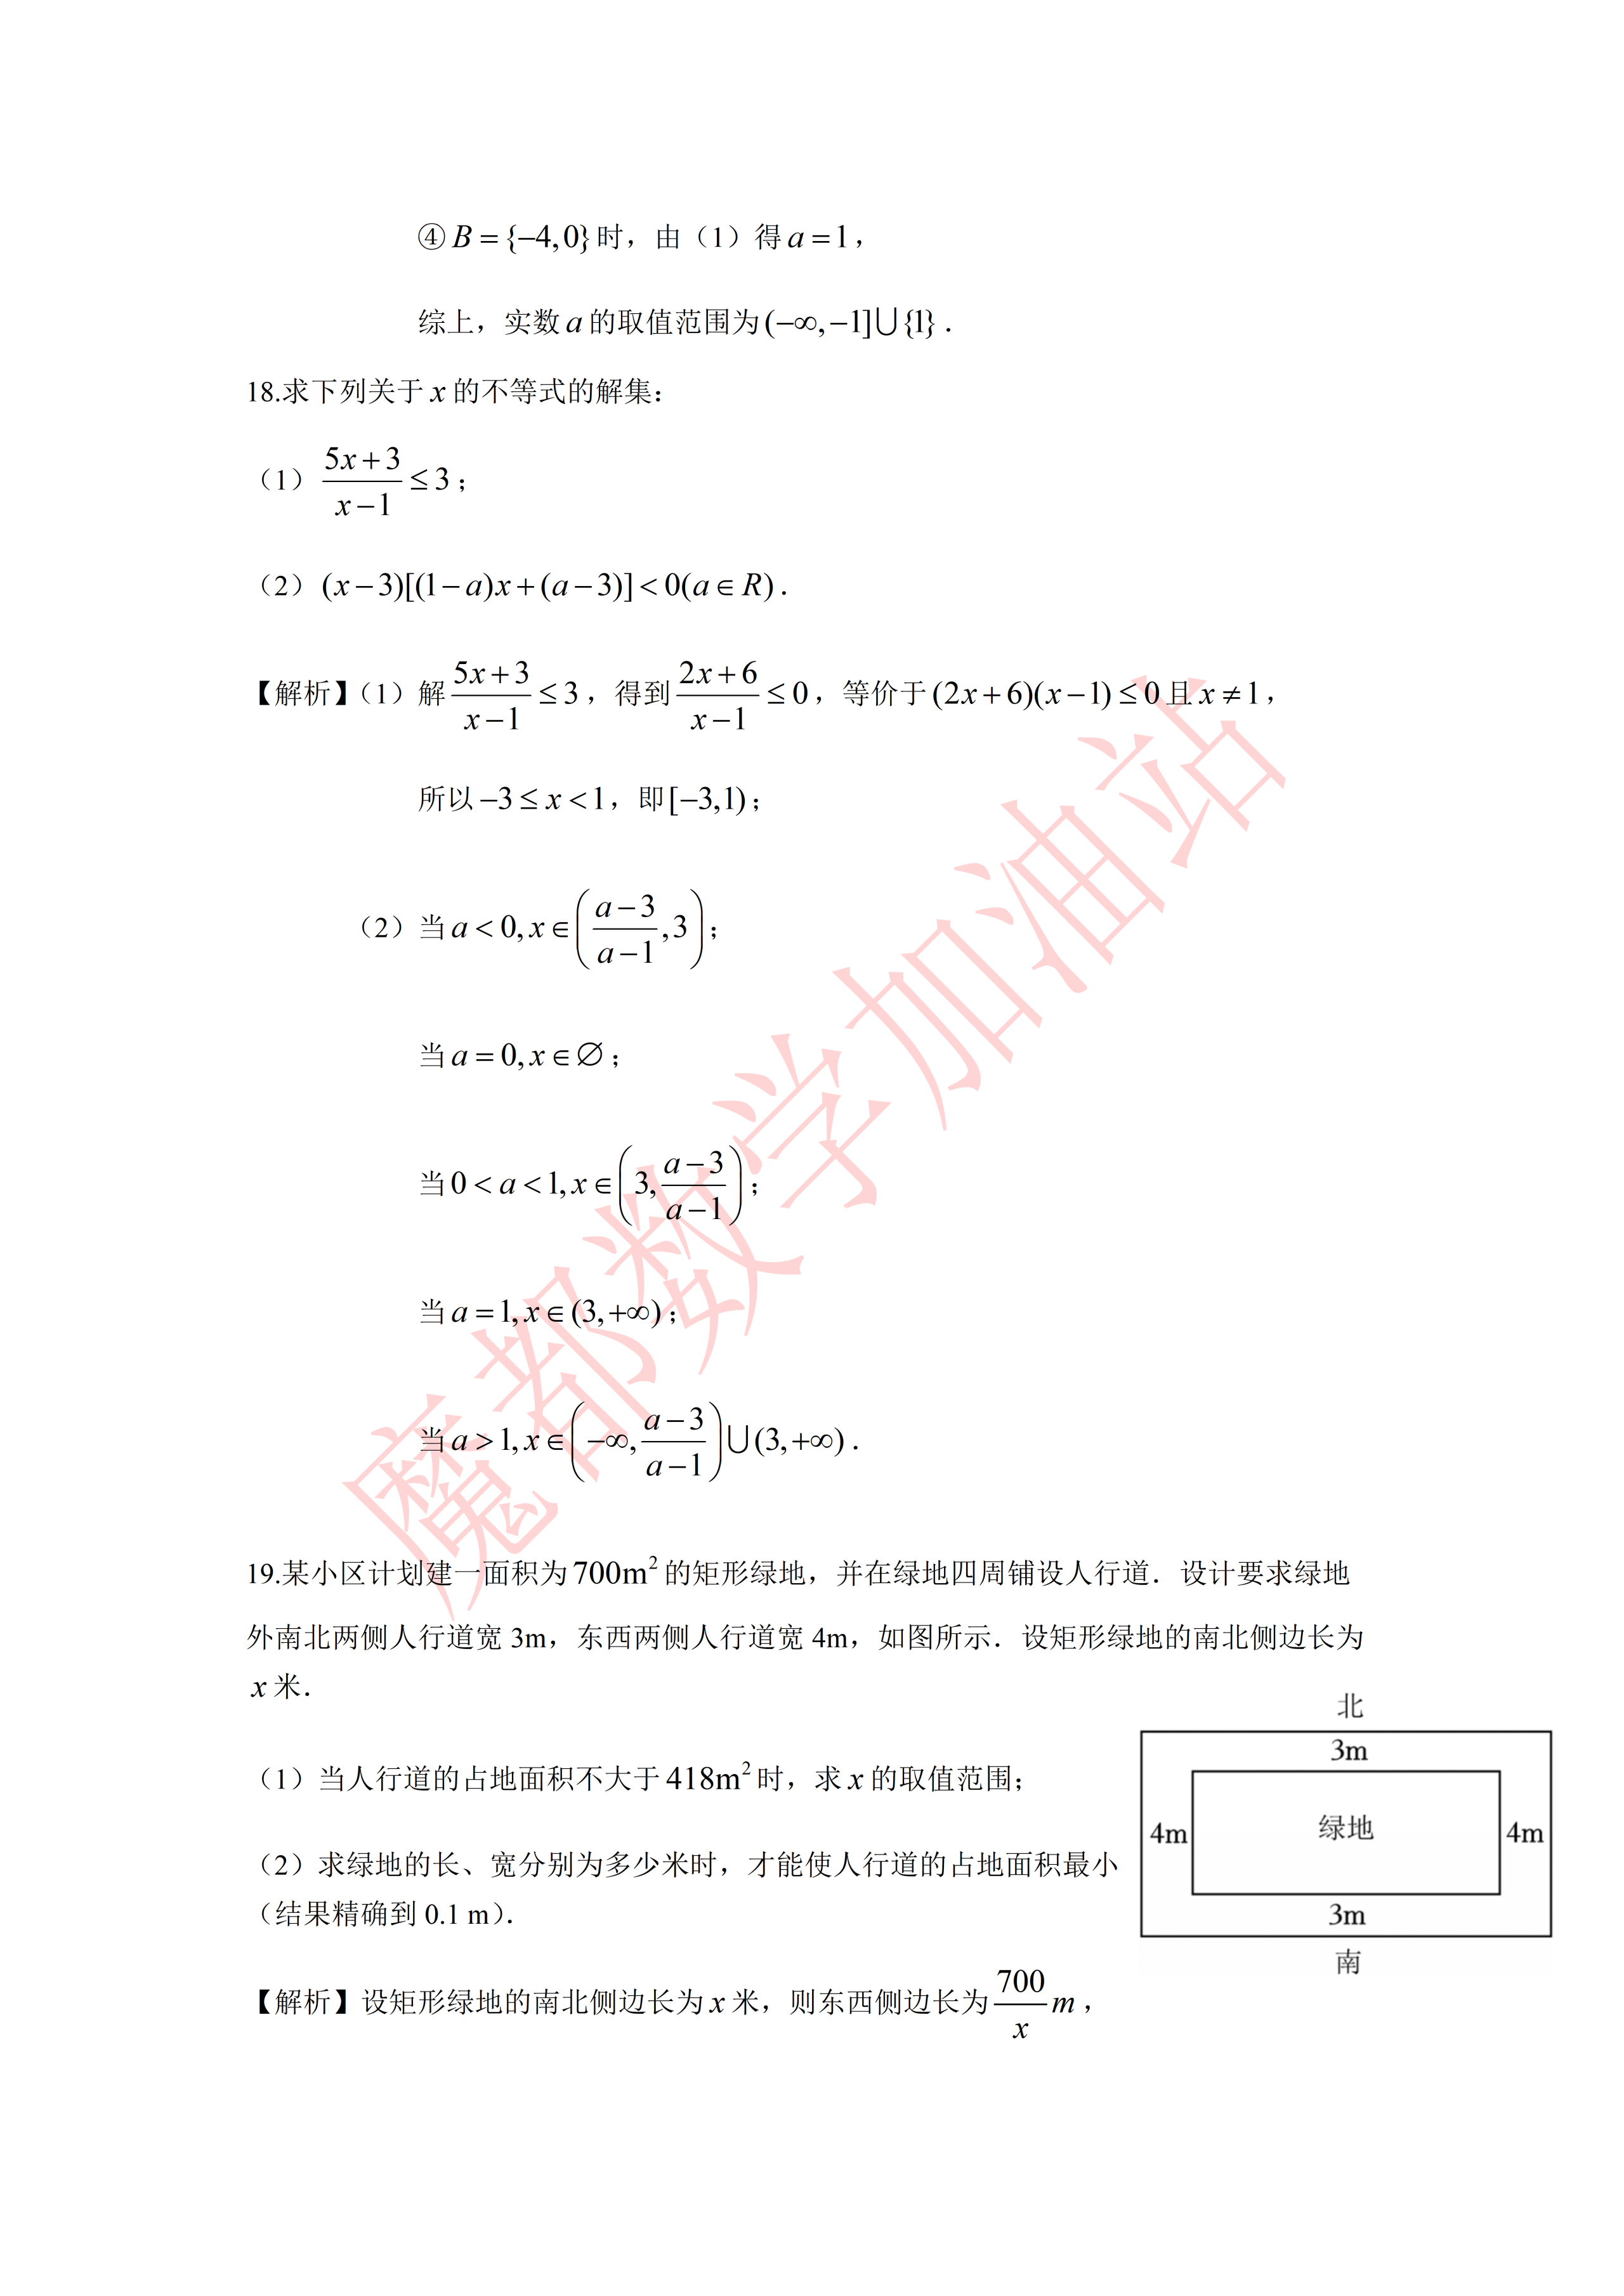
\includegraphics[width=.3\linewidth,trim=1791bp 484bp 107bp 2654bp,clip]{../原图/高一53_华师大二附中_10月月考/07.png}
\end{center}

\begin{enumerate}[label=(\arabic*)]
\item 当人行道的占地面积不大于 $418m^2$ 时，求 $x$ 的取值范围；
\item 求绿地的长、宽分别为多少米时，才能使人行道的占地面积最小（结果精确到 $0.1m$）.
\end{enumerate}

\ifanswer
\solbegin
\step{设矩形绿地的南北侧边长为 $x$ 米，则东西侧边长为 $\dfrac{700}{x}m$，}
\step{则人行道的占地面积为 $S=(x+8)\left(\dfrac{700}{x}+6\right)-700$，即 $S=6x+\dfrac{5600}{x}+48$.}
\stepm{(1)}{当人行道的占地面积不大于 $418m^2$ 时，$6x+\dfrac{5600}{x}+48\leqslant418$，}
\step{即 $6x^2-370x+5600\leqslant0$，解得 $\dfrac{80}{3}\leqslant x\leqslant35$，}
\step{故当人行道的占地面积不大于 $418m^2$ 时，$x\in\left[\dfrac{80}{3},35\right]$；}
\stepm{(2)}{$S=6x+\dfrac{5600}{x}+48\geqslant2\sqrt{6x\cdot\dfrac{5600}{x}}+48=80\sqrt{21}+48$，}
\step{当且仅当 $6x=\dfrac{5600}{x}$，即 $x=20\sqrt{\dfrac73}\approx30.6(m)$ 时，}
% 原卷如此，照录未改（80√21+48≈414.6，两处“414.4”疑笔误，见文件头“原卷笔误/存疑”第 6 条）
\step{$S$ 达到最小值 $80\sqrt{21}+48\approx414.4$，此时 $\dfrac{700}{x}\approx22.9(m)$，}
\step{所以当设计绿地的南北侧边长约为 $30.6m$，东西侧边长约为 $22.9m$ 时，}
\step{人行道的占地面积最小值为 $414.4(m^2)$.}
\solend
\fi

\ansspace[6]

\item 已知 $x\in\R$，符号 $[x]$ 表示不大于 $x$ 的最大整数，例如：$[2.3]=2$,$[2]=2$，$[-1.2]=-2$，令 $S(x)=[x]-[-x]$.

\begin{enumerate}[label=(\arabic*)]
\item 写出 $S(x)$ 为偶数（包括正、负偶数和 0）的充要条件，并证明；
\item 设方程 $|S(x)|=3$ 的解集为 $A$.

①集合 $B=\{x\mid x^2-ax-9\leqslant0,a\in\R\}$，若 $A\cap B=A$，求实数 $a$ 的取值范围；

②集合 $C=\{x\mid 2x^2-5kx+3k^2\geqslant0\}$，若 $A\cup C=\R$，求实数 $k$ 的取值范围.
\end{enumerate}

\ifanswer
\solbegin
\stepm{(1)}{$S(x)$ 为偶数的充要条件是 $x\in\Z$.}
\step{若 $x\in\Z$，则 $S(x)=[x]-[-x]=x-(-x)=2x$；}
\step{若 $x\notin\Z$，设 $[x]=n$，}
\step{则 $S(x)=[x]-[-x]=n-(-n-1)=2n+1=2[x]+1$；}
% 原卷如此，照录未改（“由①”按文意应为“由(1)”，见文件头“原卷笔误/存疑”第 3 条）
\stepm{(2)}{由①得 3 是奇数，$S(x)=\pm3$,$x\notin\Z$，}
\step{$S(x)=2[x]+1=\pm3$,$[x]=1$ 或 $-2$ 且 $x\notin\Z$，}
\step{所以 $A=(-2,-1)\cup(1,2)$；}
\stepm{①}{$A\cap B=A\Rightarrow A\subseteq B$，}
\step{设 $B=[x_1,x_2]$，其中 $x_1,x_2$ 是方程 $x^2-ax-9=0$ 的两实根，}
\step{设 $f(x)=x^2-ax-9$，}
\step{$[-2,2]\subseteq[x_1,x_2]\Leftrightarrow x_1\leqslant-2$,$x_2\geqslant2\Leftrightarrow\begin{cases}f(-2)\leqslant0\\ f(2)\leqslant0\end{cases}$}
\step{$\Leftrightarrow\begin{cases}(-2)^2-a\cdot(-2)-9\leqslant0, & a\leqslant\dfrac52\\ 2^2-2a-9\leqslant0, & a\geqslant-\dfrac52\end{cases}$，故 $a\in\left[-\dfrac52,\dfrac52\right]$；}
\step{注：若用求根公式 $\begin{cases}\dfrac{a+\sqrt{a^2+36}}{2}\geqslant2\Rightarrow a\geqslant-\dfrac52\\ \dfrac{a-\sqrt{a^2+36}}{2}\leqslant-2\Rightarrow a\leqslant\dfrac52\end{cases}$，结果正确，也得满分；}
\stepm{②}{$2x^2-5kx+3k^2=(x-k)(2x-3k)$.}
\step{$A\cup C=\R\Leftrightarrow\complement_\R A\subseteq C$.}
\step{记 $g(x)=2x^2-5kx+3k^2$，则 $\{x\mid g(x)<0\}\subseteq A$.}
\stepm{情况1：}{$k>0$ 时，$k<\dfrac32k$,$g(x)<0$ 的解集为 $\left(k,\dfrac32k\right)\subseteq(1,2)$，}
\step{故 $\begin{cases}k\geqslant1\\ \dfrac32k\leqslant2\end{cases}\Rightarrow1\leqslant k\leqslant\dfrac43$；}
\stepm{情况2：}{$k=0$ 时，$g(x)=2x^2\geqslant0$ 恒成立，$C=\R$,$A\cup C=\R$ 显然成立；}
\stepm{情况3：}{$k<0$ 时，$\dfrac32k<k$,$g(x)<0$ 的解集为 $\left(\dfrac32k,k\right)\subseteq(-2,-1)$，}
\step{故 $\begin{cases}\dfrac32k\geqslant-2\\ k\leqslant-1\end{cases}\Rightarrow-\dfrac43\leqslant k\leqslant-1$；}
\step{综上，$k\in\left[-\dfrac43,-1\right]\cup\{0\}\cup\left[1,\dfrac43\right]$.}
\solend
\fi

\ansspace[10]

\item 对于非空实数集 $M\subseteq(0,+\infty)$，若满足以下两个条件，则称 $M$ 为“极闭集”：

①$M$ 中至少含有 2 个元素，且 $1\notin M$；

②对于 $M$ 中任意两个不相等的元素 $x,y$，定义 $x*y=\dfrac{xy+1}{x+y}$，且 $x*y\in M$.

\begin{enumerate}[label=(\arabic*)]
\item 判断集合 $A=\left\{\dfrac12,2\right\}$ 与区间 $B=(1,+\infty)$ 是否为“极闭集”，并说明理由；
\item 若 $M$ 是“极闭集”，证明：集合 $M$ 中不可能所有元素都小于 1；
\item 证明：不存在任何有限的“极闭集”.
\end{enumerate}

\ifanswer
\solbegin
% 原卷如此，照录未改（首行集合按题干应为 {1/2,2}，见文件头“原卷笔误/存疑”第 7 条）
\stepm{(1)}{对于集合 $A=\left\{\dfrac12,1\right\}$，$\dfrac12*2=\dfrac45$，}
\step{因为 $\dfrac45\notin A$，不满足条件②，所以集合 $A$ 不是“极闭集”.}
\step{对于区间 $B$，满足条件①.}
\step{任取 $B$ 中两个不相等的元素 $x,y$，则 $x>1$,$y>1$.}
\step{$x*y-1=\dfrac{xy+1}{x+y}-1=\dfrac{(x-1)(y-1)}{x+y}>0$，所以 $x*y>1$，}
\step{这说明 $x*y\in B$ 恒成立，满足条件②，所以 $B$ 是“极闭集”.}
\stepm{(2)}{假设集合 $M$ 中所有元素都小于 1，}
\step{在 $M$ 中取 $0<x<y<1$,$x*y-1=\dfrac{xy+1}{x+y}-1=\dfrac{(x-1)(y-1)}{x+y}>0$，}
\step{所以 $x*y>1$，与“集合 $M$ 中所有元素都小于 1”矛盾，}
\step{假设不成立，集合 $M$ 中不可能所有元素都小于 1，得证.}
\stepm{(3)}{由②得，任何一个“极闭集”$M$ 中，必然至少存在一个大于 1 的元素，}
\stepm{情况1：}{若 $M$ 中至少存在两个大于 1 的元素，}
\step{设其中两个不相等的元素为 $x$ 和 $y_1$，且 $x>y_1>1$，}
\step{令 $y_{n+1}=x*y_n$,$n\geqslant1$,$y_{n+1}-1=x*y_n-1=\dfrac{(x-1)(y_n-1)}{xy_n+1}>0$，}
\step{如果 $y_n\geqslant1$，则显然 $y_{n+1}\geqslant1$，作差 $y_n-y_{n+1}=\dfrac{y_n^2-1}{x+y_n}>0$，}
\step{由此 $x>y_1>y_2>y_3>\cdots>1$，与有限集矛盾.}
\stepm{情况2：}{若 $M$ 中恰好只有一个元素大于 1，}
\step{设这个唯一大于 1 的元素为 $m$.}
\step{因为 $M$ 至少有两个元素，所以 $M$ 中必然至少存在一个元素 $a_1<1$，}
\step{令 $a_{n+1}=m*a_n$,$n\geqslant1$，}
\step{又 $a_{n+1}-1=m*a_n-1=\dfrac{(m-1)(a_n-1)}{m+a_n}<0$，故 $a_{n+1}<1$，}
\step{作差 $a_{n+1}-a_n=\dfrac{1-a_n^2}{m+a_n}>0$，由此 $a_1<a_2<a_3<\cdots<1$，与有限集矛盾.}
\step{因此，不存在任何有限的“极闭集”. 原命题得证.}
\solend
\fi

\ansspace*[10]

\end{enumerate}

\end{document}
"
% 紧凑版：xelatex "\def\iscompact{1}% 高一53_华师大二附中_10月月考.tex
%   —— 高一上数学“2026-2027 年华师大二附中高一上 10 月月考”（讲评版）
% 试卷版：xelatex 高一53_华师大二附中_10月月考.tex
% 答案版：xelatex "\def\isanswer{1}\input{高一53_华师大二附中_10月月考.tex}"
% 紧凑版：xelatex "\def\iscompact{1}\input{高一53_华师大二附中_10月月考.tex}"
%
% 原始材料：微信公众号“魔都数学加油站”文章，作者破晓，连载“27学年高一53”；
% 原文标题“27学年高一53——2026-2027年上海市华师大二附中高一上10月月考”；
% 原文链接：https://mp.weixin.qq.com/s/fpSnoF-gJEEWyxAoPC_bZA。
% 页面标注发布时间 2026-10-09 17:15（上海）。
% 正文为 11 张 PNG 页：第 01—06、08、10 页 4762×6735，第 07、09、11 页 2560×3620
% （**同一篇各页分辨率不同**），均按页序读取。11 页全为试卷正文页（卷首标题在第 1 页页顶，
% 卷末解答题第 21 题解析止于第 11 页），无封面页、目录页、二维码或宣传页。
% 粉色斜排“魔都数学加油站”为卷面水印，与公众号页脚一并未录入。
%
% 卷首标题：照卷面印作“2026--2027 年华师大二附中高一上 10 月月考”（公众号标题中的“上海市”
% 卷面标题行没有，本稿照卷面），年份区间按全稿惯例排 en dash。原卷只有一行标题、无副标题。
%
% 篇幅与题号：原卷自第 3 题起编号（第 1、2 题不在本卷内）。填空题 3—12（10 题）、
% 选择题 13—16（4 题）、解答题 17—21（5 题），共 19 题。本稿沿用原节与原题号，
% 只改排为全稿统一的大节样式（原卷小节标题为“一、填空题”“二、选择题”“三、解答题”）。
%
% 讲评版：原卷每题下直接印【答案】或【解析】。**第 13 题没有任何【答案】/【解析】段**，
% 答案“C”直接印在题干括号内（“一定不是(  C  )”），本稿按 高一37 第 13 题的成例把括号留空、
% 答案另提为 \ans{$C$}；其余 18 题都只印【解析】，按全稿口径这类题不另提 \ans{}——其中
% 选择题第 14、15、16 题的结论写在解析末句（“故选 B／D／C”），亦照录在解析内。
%
% 副标题：原卷未印副标题。本稿按“知识模块”口径标作“集合与常用逻辑用语、不等式”：
% 19 题中集合与常用逻辑用语 12 题（集合类 9 题——第 4、5、12、13、15、16、17、20、21 题；
% 逻辑类 3 题——第 3、9、14 题），不等式 7 题（含一元二次方程与绝对值方程：第 6、7、8、10、
% 11、18、19 题，其中第 11 题实为奇偶分析下的集合计数题，暂挂不等式），两类均超三分之一，
% 故并标。口径同 高一46、高一47、高一48、高一51、高一52。
%
% 与原卷的排版差异：
%   ① 原卷每题下直接印【解析】，本稿按全稿惯例将答案与解析置于答案版，试卷版保持干净；
%      第 13 题印在题干括号内的答案“C”同样移入 \ans{}，见上；
%   ② 原卷未印副标题，本稿按“知识模块”口径补出；
%   ③ 原卷填空横线约两个字宽，本稿按全稿惯例统一排 \blankline[4.4em]；
%      选择题的作答括号原卷排半角“(    )”，本稿按全稿惯例排 \mbox{（\quad）}；
%   ④ 原卷实数集排斜体/粗体 $R$、$\mathbf{R}$（第 4、6、7、18、20 题等处），本稿按全稿惯例
%      改用 $\R$；空集记号统一为 \varnothing；
%   ⑤ 原卷在数学式内多处用半角逗号（如 $x_1,x_2$、$|S|,|T|$、$a\neq0,c\neq0$），均照录未强改；
%      句末句点按全稿惯例排西文句点（原卷“故选 B．”一类全角句点亦从宽排作“.”）；
%   ⑥ 第 17—21 题的子问原卷各自另起一行，本稿按全稿惯例用 enumerate 的 (1)(2)(3)；
%      第 20 题 (2) 问下的①②两行是题干的一部分，照录为行首①②标号（不入 enumerate）；
%      解析中的子问标号一律用 \stepm{(1)}{…}，解析中的①②③④分情形用 \stepm{①}{…}；
%   ⑦ 第 12、20、21 题解析里的“情况1:”至“情况3:”标号原卷排**红色加粗**（全卷共 6 处），
%      全库无红色排字先例，本稿按全稿子题标号样式排 \stepm{情况1：}{…}（加粗着色、不改黑色基调），
%      冒号照原卷排全角；
%   ⑧ 第 19 题的示意图原卷排在题干右侧（与题干、(1) 问同高），本稿居中排在题干之后、
%      子问之前，并在 \item 前加 \needvspace 整块推走；图自原图第 07 页裁切（trim），不另存图片文件；
%   ⑨ 每道解答题原卷未留作答空白，本稿按全稿惯例加 \ansspace。
%
% 原卷笔误/存疑（均照录未改，正文对应处另有 % 注）：
%   1. 第 14 题解析末行“例如 $a=1$，$b=-1$，及必要性不成立”，“及”按文意应为“即”；
%   2. 第 15 题解析第 3 行 $\dfrac1{a+b\sqrt2}=\dfrac a{a^2-2b}+\left(-\dfrac b{a^2-2b}\right)\cdot\sqrt2$，
%      分母两处均作 $a^2-2b$，按通分应为 $a^2-2b^2$（结论 $C=X$ 不受影响）；
%   3. 第 20 题 (2) 问解析首行“由①得 3 是奇数”，按文意应为“由(1)得”（①是 (2) 问下自己
%      的子问标号，奇偶性结论出自 (1) 问）；
%   4. 第 11 题解析“只有奇数的有 $C_4^2+1=7$ 个”，按组合意义应为 $C_4^2+C_4^4=7$
%      （“$+1$”当指 4 个奇数全取的 1 种），数值无误；
%   5. 第 18 题 (2) 问解析“当 $a=0$,$x\in\varnothing$”，按文意应为“解集为 $\varnothing$”；
%   6. 第 19 题 (2) 问解析“$S$ 达到最小值 $80\sqrt{21}+48\approx414.4$”与末行
%      “人行道的占地面积最小值为 $414.4(m^2)$”，两处按 $80\sqrt{21}+48\approx414.6$，疑笔误；
%   7. 第 21 题 (1) 问解析首行“对于集合 $A=\left\{\frac12,1\right\}$”，按题干应为
%      $A=\left\{\frac12,2\right\}$（计算 $\frac12*2=\frac45$ 用的正是 $2$）；
%   8. 第 12 题解析“所以 $A=(-\infty,-4]\cup[2,+\infty)$”一行行末无标点，体例不一，照录。
%
% 插图：1 张，自原图裁切（无 \begin{tikzpicture} 重排）：
%   · 第 19 题绿地示意图（外矩形内套矩形“绿地”，上“北 3m”、下“南 3m”、左右各“4m”）
%     ——原图第 07 页，原卷排于题干右侧。
%     裁框：x 1797–2447、y 2660–3136（含“北”“南”标注，四周各留约 6px），
%     trim=1791bp 484bp 107bp 2654bp（左／下／右／上），页宽 2560、页高 3620。
%
\documentclass[a4paper,11pt]{article}
\usepackage{common}

\begin{document}

\examtitlest[3]{2026--2027 年华师大二附中高一上 10 月月考}{集合与常用逻辑用语、不等式}

\bigsec{一、填空题}

\begin{enumerate}
\setcounter{enumi}{2}

\item “$x=2$”是“$x^2-3x+2=0$”的\blankline[4.4em]条件.

（选择其中之一填空：充分非必要、必要非充分、充分、既非充分又非必要）

\ifanswer
\solbegin
\step{由 $x^2-3x+2=0$ 得 $x=1$ 或 $x=2$，}
\step{则“$x=2$”是“$x^2-3x+2=0$”的充分不必要条件.}
\solend
\fi

\item 已知 $R$ 是全集，集合 $A=\{y\mid y=-x^2+1,x\in\R\}$，集合 $B=\{x\mid x=3+|a|,a\in\R\}$，则 $\overline{A\cup B}=$\blankline[4.4em].

\ifanswer
\solbegin
\step{$A=\{y\mid y=-x^2+1,x\in\R\}=(-\infty,1]$，$B=\{x\mid x=3+|a|,a\in\R\}=[3,+\infty)$，}
\step{所以 $\overline{A\cup B}=(1,3)$.}
\solend
\fi

\item 已知 $a$ 为常数，集合 $A=\{x\mid x^2+x-6=0\}$，集合 $B=\{x\mid ax-2=0\}$，且 $B\subseteq A$，则 $a$ 的所有取值构成的集合为\blankline[4.4em].

\ifanswer
\solbegin
\step{集合 $A=\{-3,2\}$，因为 $B\subseteq A$，则 $B=\varnothing$，$\{-3\}$，$\{2\}$，$\{-3,2\}$，}
\step{当 $B=\varnothing$ 时，$a=0$，当 $B=\{-3\}$ 时，$a=-\dfrac23$，当 $B=\{2\}$ 时，$a=1$，}
\step{当 $B=\{-3,2\}$ 时，不成立，故 $a$ 的取值集合为 $\left\{0,-\dfrac23,1\right\}$.}
\solend
\fi

\item 设 $a\in\R$，若关于 $x$ 的不等式 $x^2-ax<0$ 的解集是区间 $(0,1)$ 的真子集，则 $a$ 的取值范围是\blankline[4.4em].

\ifanswer
\solbegin
\step{因为关于 $x$ 的不等式 $x^2-ax<0$ 的解集是区间 $(0,1)$ 的真子集，}
\step{当 $a=0$ 时，不等式的解集为 $\varnothing$，符合题意；}
\step{当 $a>0$ 时，不等式的解集为 $(0,a)$，则 $0<a<1$，}
\step{当 $a<0$ 时，不等式的解集为 $(a,0)$，不符合题意，}
\step{故 $a$ 的范围为 $[0,1)$.}
\solend
\fi

\item 设 $x\in\R$，则方程 $|2x+3|-|x-2|=|3x+1|$ 的解集为\blankline[4.4em].

\ifanswer
\solbegin
\step{当 $x\leqslant-\dfrac32$ 时，原式$\Leftrightarrow-2x-3+x-2=-3x-1\Leftrightarrow x=2$，不合题意；}
\step{当 $-\dfrac32<x\leqslant-\dfrac13$ 时，原式$\Leftrightarrow2x+3+x-2=-3x-1\Leftrightarrow x=-\dfrac13$；}
\step{当 $-\dfrac13<x\leqslant2$ 时，原式$\Leftrightarrow2x+3+x-2=3x+1\Leftrightarrow1=1$ 即恒成立；}
\step{当 $x>2$ 时，原式$\Leftrightarrow2x+3+2-x=3x+1\Leftrightarrow x=2$，不合题意；}
\step{故 $x\in\left[-\dfrac13,2\right]$.}
\solend
\fi

\item 已知关于 $x$ 的一元二次方程 $x^2+(4m+1)x+2m-1=0$．若方程的两根为 $x_1$、$x_2$，且满足 $\dfrac1{x_1}+\dfrac1{x_2}=-\dfrac12$，则实数 $m=$\blankline[4.4em].

\ifanswer
\solbegin
\step{由于判别式$\Delta=16m^2+5>0$恒成立，}
\step{不论 $m$ 为任何实数，方程总有两个不相等的实数根.}
\step{$\dfrac1{x_1}+\dfrac1{x_2}=-\dfrac12$，即 $\dfrac{x_1+x_2}{x_1x_2}=-\dfrac12$，由根与系数的关系得 $\dfrac{-4m-1}{2m-1}=-\dfrac12$，}
\step{解得 $m=-\dfrac12$.}
\solend
\fi

\item 已知 $\dfrac1{x-2}\geqslant1$ 是 $|x-a|<2$ 的充分非必要条件，则实数 $a$ 的取值范围是\blankline[4.4em].

\ifanswer
\solbegin
\step{由 $\dfrac1{x-2}\geqslant1$ 得 $\dfrac{3-x}{x-2}\geqslant0$，解得 $2<x\leqslant3$，由 $|x-a|<2$ 得 $a-2<x<a+2$，}
\step{因为 $\dfrac1{x-2}\geqslant1$ 是 $|x-a|<2$ 的充分非必要条件，}
\step{所以 $\{x\mid 2<x\leqslant3\}\subset\{x\mid a-2<x<a+2\}$，所以 $\begin{cases}a-2\leqslant2\\ a+2>3\end{cases}$，解得 $1<a\leqslant4$，}
\step{即实数 $a$ 的取值范围是 $(1,4]$.}
\solend
\fi

\item 设 $x,y\in(0,+\infty)$，且 $x+4y=1$，则 $\dfrac1x+\dfrac1y$ 的最小值为\blankline[4.4em].

\ifanswer
\solbegin
\step{因为 $\dfrac1x+\dfrac1y=(x+4y)\left(\dfrac1x+\dfrac1y\right)=5+\dfrac{4y}{x}+\dfrac{x}{y}\geqslant5+2\sqrt{\dfrac{4y}{x}\cdot\dfrac{x}{y}}=9$，}
\step{当且仅当 $\dfrac{4y}{x}=\dfrac{x}{y}$，即 $x=2y$，即 $x=\dfrac13$,$y=\dfrac16$ 时取等号，故最小值为 $9$.}
\solend
\fi

\item 设非空集合 $Q\subseteq M$，当 $Q$ 中所有元素和为偶数时（集合为单元素时和为元素本身），称 $Q$ 是 $M$ 的偶子集. 若集合 $M=\{1,2,3,4,5,6,7\}$，则其偶子集 $Q$ 的个数为\blankline[4.4em].

\ifanswer
\solbegin
\step{偶子集可以分为只有奇数、偶数及偶数个奇数和偶数的集合，}
\step{奇数有 4 个，偶数有 3 个，}
% 原卷如此，照录未改：按组合意义应为 C_4^2+C_4^4=7（“+1”当指 4 个奇数全取的 1 种），
% 见文件头“原卷笔误/存疑”第 4 条
\step{只有奇数的有 $C_4^2+1=7$ 个，只有偶数的有 $C_3^1+C_3^2+1=7$ 个，}
\step{偶数个奇数和偶数的：两奇一偶 $C_4^2\cdot C_3^1=18$ 个，两奇二偶 $C_4^2\cdot C_3^2=18$ 个，}
\step{两奇三偶 $C_4^2\cdot C_3^3=6$ 个，四奇一偶 $C_4^4\cdot C_3^1=3$ 个，四奇二偶 $C_4^4\cdot C_3^2=3$ 个，}
\step{四奇三偶 $C_4^4\cdot C_3^3=1$ 个，所以共有 $7+7+18+18+6+3+3+1=63$ 个.}
\solend
\fi

\item 已知集合 $A=\{x\mid x^2+2x-8\geqslant0\}$,$B=\{x\mid x^2-2ax+2a\leqslant0\}$，且 $A\cap B$ 中恰有 3 个整数元素，则实数 $a$ 的取值范围为\blankline[4.4em].

\ifanswer
\solbegin
% 原卷如此，照录未改：此行行末无标点，见文件头“原卷笔误/存疑”第 8 条
\step{由 $x^2+2x-8\geqslant0$，得 $x\geqslant2$ 或 $x\leqslant-4$，所以 $A=(-\infty,-4]\cup[2,+\infty)$}
\step{对集合 $B$：$x^2-2ax+2a\leqslant0$,$\Delta=4a^2-8a=4a(a-2)\geqslant0$，}
\step{得 $a\leqslant0$ 或 $a\geqslant2$.}
\step{设方程 $x^2-2ax+2a=0$ 的两根为 $r_1,r_2$，}
\step{则 $B=[r_1,r_2]$,$r_1=a-\sqrt{a^2-2a}$,$r_2=a+\sqrt{a^2-2a}$，}
\stepm{情况1：}{$a\leqslant0$，}
\step{$r_2=a+\sqrt{a^2-2a}<a+\sqrt{a^2-2a+1}=a+|a-1|=a+1-a=1<2$，}
\step{$B$ 只在 $A$ 的左侧部分有交集，要使 $A\cap B$ 恰有 3 个整数元素，}
\step{这 3 个整数为 $-6,-5,-4$，于是 $r_1\in(-7,-6]$，}
\step{令 $f(x)=x^2-2ax+2a$，则 $\begin{cases}f(-7)=49+14a+2a>0\\ f(-6)=36+12a+2a\leqslant0\end{cases}\Rightarrow a\in\left(-\dfrac{49}{16},-\dfrac{18}{7}\right]$；}
\stepm{情况2：}{$a\geqslant2$，}
\step{$r_2=a+\sqrt{a^2-2a}\geqslant2$，}
\step{$r_1=a-\sqrt{a^2-2a}>a-\sqrt{a^2-2a+1}=a-|a-1|=a-(a-1)=1>-4$，}
\step{所以 $A\cap B=[2,r_2]$.}
\step{同理 $\begin{cases}f(4)=16-8a+2a\leqslant0\\ f(5)=25-10a+2a>0\end{cases}\Rightarrow a\in\left[\dfrac{8}{3},\dfrac{25}{8}\right)$；}
\step{综上，$a\in\left(-\dfrac{49}{16},-\dfrac{18}{7}\right]\cup\left[\dfrac{8}{3},\dfrac{25}{8}\right)$.}
\solend
\fi

\end{enumerate}

\bigsec{二、选择题}

\begin{enumerate}
\setcounter{enumi}{12}

% 第 13 题原卷无【答案】/【解析】段，答案“C”直接印在题干括号内，
% 按高一37 第 13 题的成例括号留空、答案另提为 \ans{}（见文件头）
\item 集合 $A=\{a,b,c\}$ 中的三个元素分别表示某一个三角形的三边长度，那么这个三角形一定不是\mbox{（\quad）}

\keepwithprev
A. 锐角三角形\qquad B. 钝角三角形

C. 等腰三角形\qquad D. 直角三角形

\ifanswer
\ans{$C$}
\fi

\item 设 $a$、$b$ 为实数，则“$a<b<0$”是“$\dfrac1a>\dfrac1b$”的\mbox{（\quad）}条件.

\keepwithprev
A. 充要\qquad B. 充分不必要

C. 必要不充分\qquad D. 既不充分也不必要

\ifanswer
\solbegin
\step{若 $a<b<0$，则 $\dfrac1a>\dfrac1b$ 一定成立，即充分性成立；}
% 原卷如此，照录未改（“及”按文意应为“即”，见文件头“原卷笔误/存疑”第 1 条）
\step{若 $\dfrac1a>\dfrac1b$ 成立，$a<b<0$ 不一定成立，例如 $a=1$，$b=-1$，及必要性不成立.}
\step{故选 $B$.}
\solend
\fi

\item 设 $Q$ 表示有理数集，集合 $X=\{x\mid x=a+b\sqrt2,a,b\in Q,x\neq0\}$，在下列集合中：①$\{2x\mid x\in X\}$②$\left\{\dfrac{x}{\sqrt2}\mid x\in X\right\}$③$\left\{\dfrac1x\mid x\in X\right\}$④$\{x^2\mid x\in X\}$，与 $X$ 相同的集合有\mbox{（\quad）}

\keepwithprev
A. ①②③④\qquad B. ②③④\qquad C. ①②④\qquad D. ①②③

\ifanswer
\solbegin
\step{$A=\{2x\mid x\in X\}$，$2(a+b\sqrt2)=p+q\sqrt2$ 得 $p=2a$，$q=2b$，$a=\dfrac p2$，$b=\dfrac q2$，}
\step{也是一一对应，$A=X$}
% 原卷如此，照录未改：分母两处均作 a^2-2b，按通分应为 a^2-2b^2，
% 见文件头“原卷笔误/存疑”第 2 条
\step{集合 $B=\left\{\dfrac{x}{\sqrt2}\mid x\in X\right\}$，$\dfrac{a+b\sqrt2}{\sqrt2}=b+\dfrac a2\cdot\sqrt2$，也是一一对应，$B=X$}
\step{集合 $C=\left\{\dfrac1x\mid x\in X\right\}$，$\dfrac{1}{a+b\sqrt2}=\dfrac{a}{a^2-2b}+\left(-\dfrac{b}{a^2-2b}\right)\cdot\sqrt2$，一一对应，$C=X$}
\step{集合 $D=\{x^2\mid x\in X\}$，$(a+b\sqrt2)^2=a^2+2b^2+2ab\sqrt2$，这个不能一一对应了，}
\step{集合 $D$ 包含于 $X$ 中.}
\step{故 $X$ 相同的集合有①②③，故选 $D$.}
\solend
\fi

\item 集合 $S=\{x\mid(x+a)(x^2+bx+c)=0\}$,$T=\{x\mid(ax+1)(cx^2+bx+1)=0\}$，其中 $a,b,c$ 为实数，若 $|S|,|T|$ 分别表示集合 $S,T$ 的元素个数，则 $|S|-|T|$ 的所有可能取值集合为\mbox{（\quad）}

\keepwithprev
A. $\{0\}$\qquad B. $\{1\}$\qquad C. $\{0,1\}$\qquad D. $\{-1,0,1\}$

\ifanswer
\solbegin
\stepm{①}{$a\neq0,c\neq0$ 时.}
\step{$S$ 中 $x+a=0$ 的根 $x=-a$;$T$ 中 $ax+1=0$ 的根 $x=-\dfrac1a$.}
\step{$S$ 中的 $x^2+bx+c=0$ 若无实根，则 $T$ 中的 $cx^2+bx+1=0$ 也无实根；}
\step{又设 $S$ 的 $x^2+bx+c=0$ 的根为 $r(r\neq0)$，则 $T$ 的 $cx^2+bx+1=0$ 的根为 $\dfrac1r$.}
\step{（因为 $r^2+br+c=0\Rightarrow c\cdot\left(\dfrac1r\right)^2+b\cdot\dfrac1r+1=0$）}
\step{即 $a\neq0,c\neq0$ 时，}
\step{$S$ 与 $T$ 的实根存在一一对应关系 $x\leftrightarrow\dfrac1x$,$|S|=|T|,$$|S|-|T|=0$；}
\stepm{②}{$a=0,c\neq0$ 时.}
\step{$S$ 中多出一个根 $x=0$，而 $T$ 中无此根，$|S|=|T|+1$，即 $|S|-|T|=1$；}
\stepm{③}{$a\neq0,c=0$ 时.}
\step{则 $S$ 中仍有根 $x=0$，而 $T$ 中无 0 根，同样 $|S|-|T|=1$.}
\stepm{④}{$a=0,c=0$ 时.}
\step{同样 $S$ 含有根 0，而 $T$ 中不含 0，仍有 $|S|-|T|=1$.}
\step{综上，$|S|-|T|$ 所有可能取值为 0 和 1，故选 $C$.}
\solend
\fi

\end{enumerate}

\bigsec{三、解答题}

\begin{enumerate}
\setcounter{enumi}{16}

\item 已知集合 $A=\{x\mid x^2+4x=0\}$，$B=\{x\mid x^2+2(a+1)x+a^2-1=0\}$.

\begin{enumerate}[label=(\arabic*)]
\item 若 $A$ 是 $B$ 的子集，求实数 $a$ 的值；
\item 若 $B$ 是 $A$ 的子集，求实数 $a$ 的取值范围.
\end{enumerate}

\ifanswer
\solbegin
\stepm{(1)}{因为 $A=\{-4,0\}$，$B=\{x\mid x^2+2(a+1)x+a^2-1=0\}$，又 $A\subseteq B$，}
\step{所以 $A=B$，所以 $\begin{cases}-4+0=-2(a+1)\\ -4\times0=a^2-1\end{cases}$，所以 $a=1$；}
\stepm{(2)}{因为 $B$ 是 $A$ 的子集，所以 $B=\varnothing$ 或 $B=\{-4\}$ 或 $B=\{0\}$ 或 $B=\{-4,0\}$，}
\stepm{①}{$B=\varnothing$ 时，$\Delta=4(a+1)^2-4(a^2-1)<0$，所以 $a<-1$；}
\stepm{②}{$B=\{-4\}$ 时，$\begin{cases}-4+(-4)=-2(a+1)\\ -4\times(-4)=a^2-1\end{cases}$，无解；}
\stepm{③}{$B=\{0\}$ 时，$\begin{cases}0+0=-2(a+1)\\ 0\times0=a^2-1\end{cases}$，所以 $a=-1$；}
\stepm{④}{$B=\{-4,0\}$ 时，由（1）得 $a=1$，}
\step{综上，实数 $a$ 的取值范围为 $(-\infty,-1]\cup\{1\}$.}
\solend
\fi

\ansspace[6]

\item 求下列关于 $x$ 的不等式的解集：

\begin{enumerate}[label=(\arabic*)]
\item $\dfrac{5x+3}{x-1}\leqslant3$；
\item $(x-3)[(1-a)x+(a-3)]<0$ ($a\in\R$).
\end{enumerate}

\ifanswer
\solbegin
\stepm{(1)}{解 $\dfrac{5x+3}{x-1}\leqslant3$，得到 $\dfrac{2x+6}{x-1}\leqslant0$，等价于 $(2x+6)(x-1)\leqslant0$ 且 $x\neq1$，}
\step{所以 $-3\leqslant x<1$，即 $[-3,1)$；}
\stepm{(2)}{当 $a<0$,$x\in\left(\dfrac{a-3}{a-1},3\right)$；}
% 原卷如此，照录未改（“x∈∅”按文意应为“解集为 ∅”，见文件头“原卷笔误/存疑”第 5 条）
\step{当 $a=0$,$x\in\varnothing$；}
\step{当 $0<a<1$,$x\in\left(3,\dfrac{a-3}{a-1}\right)$；}
\step{当 $a=1$,$x\in(3,+\infty)$；}
\step{当 $a>1$,$x\in\left(-\infty,\dfrac{a-3}{a-1}\right)\cup(3,+\infty)$.}
\solend
\fi

\ansspace[6]

\needvspace{13\baselineskip}

\item 某小区计划建一面积为 $700m^2$ 的矩形绿地，并在绿地四周铺设人行道. 设计要求绿地外南北两侧人行道宽 $3m$，东西两侧人行道宽 $4m$，如图所示. 设矩形绿地的南北侧边长为 $x$ 米.

\begin{center}
% 原图第 7 页题干绿地示意图直接裁取（原卷排于题干右侧）。
% 裁框取图形外框 x 1797–2447、y 2660–3136（含“北”“南”标注，四周各留约 6px），
% trim=左 1791bp／下 484bp／右 107bp／上 2654bp（页宽 2560、页高 3620）。
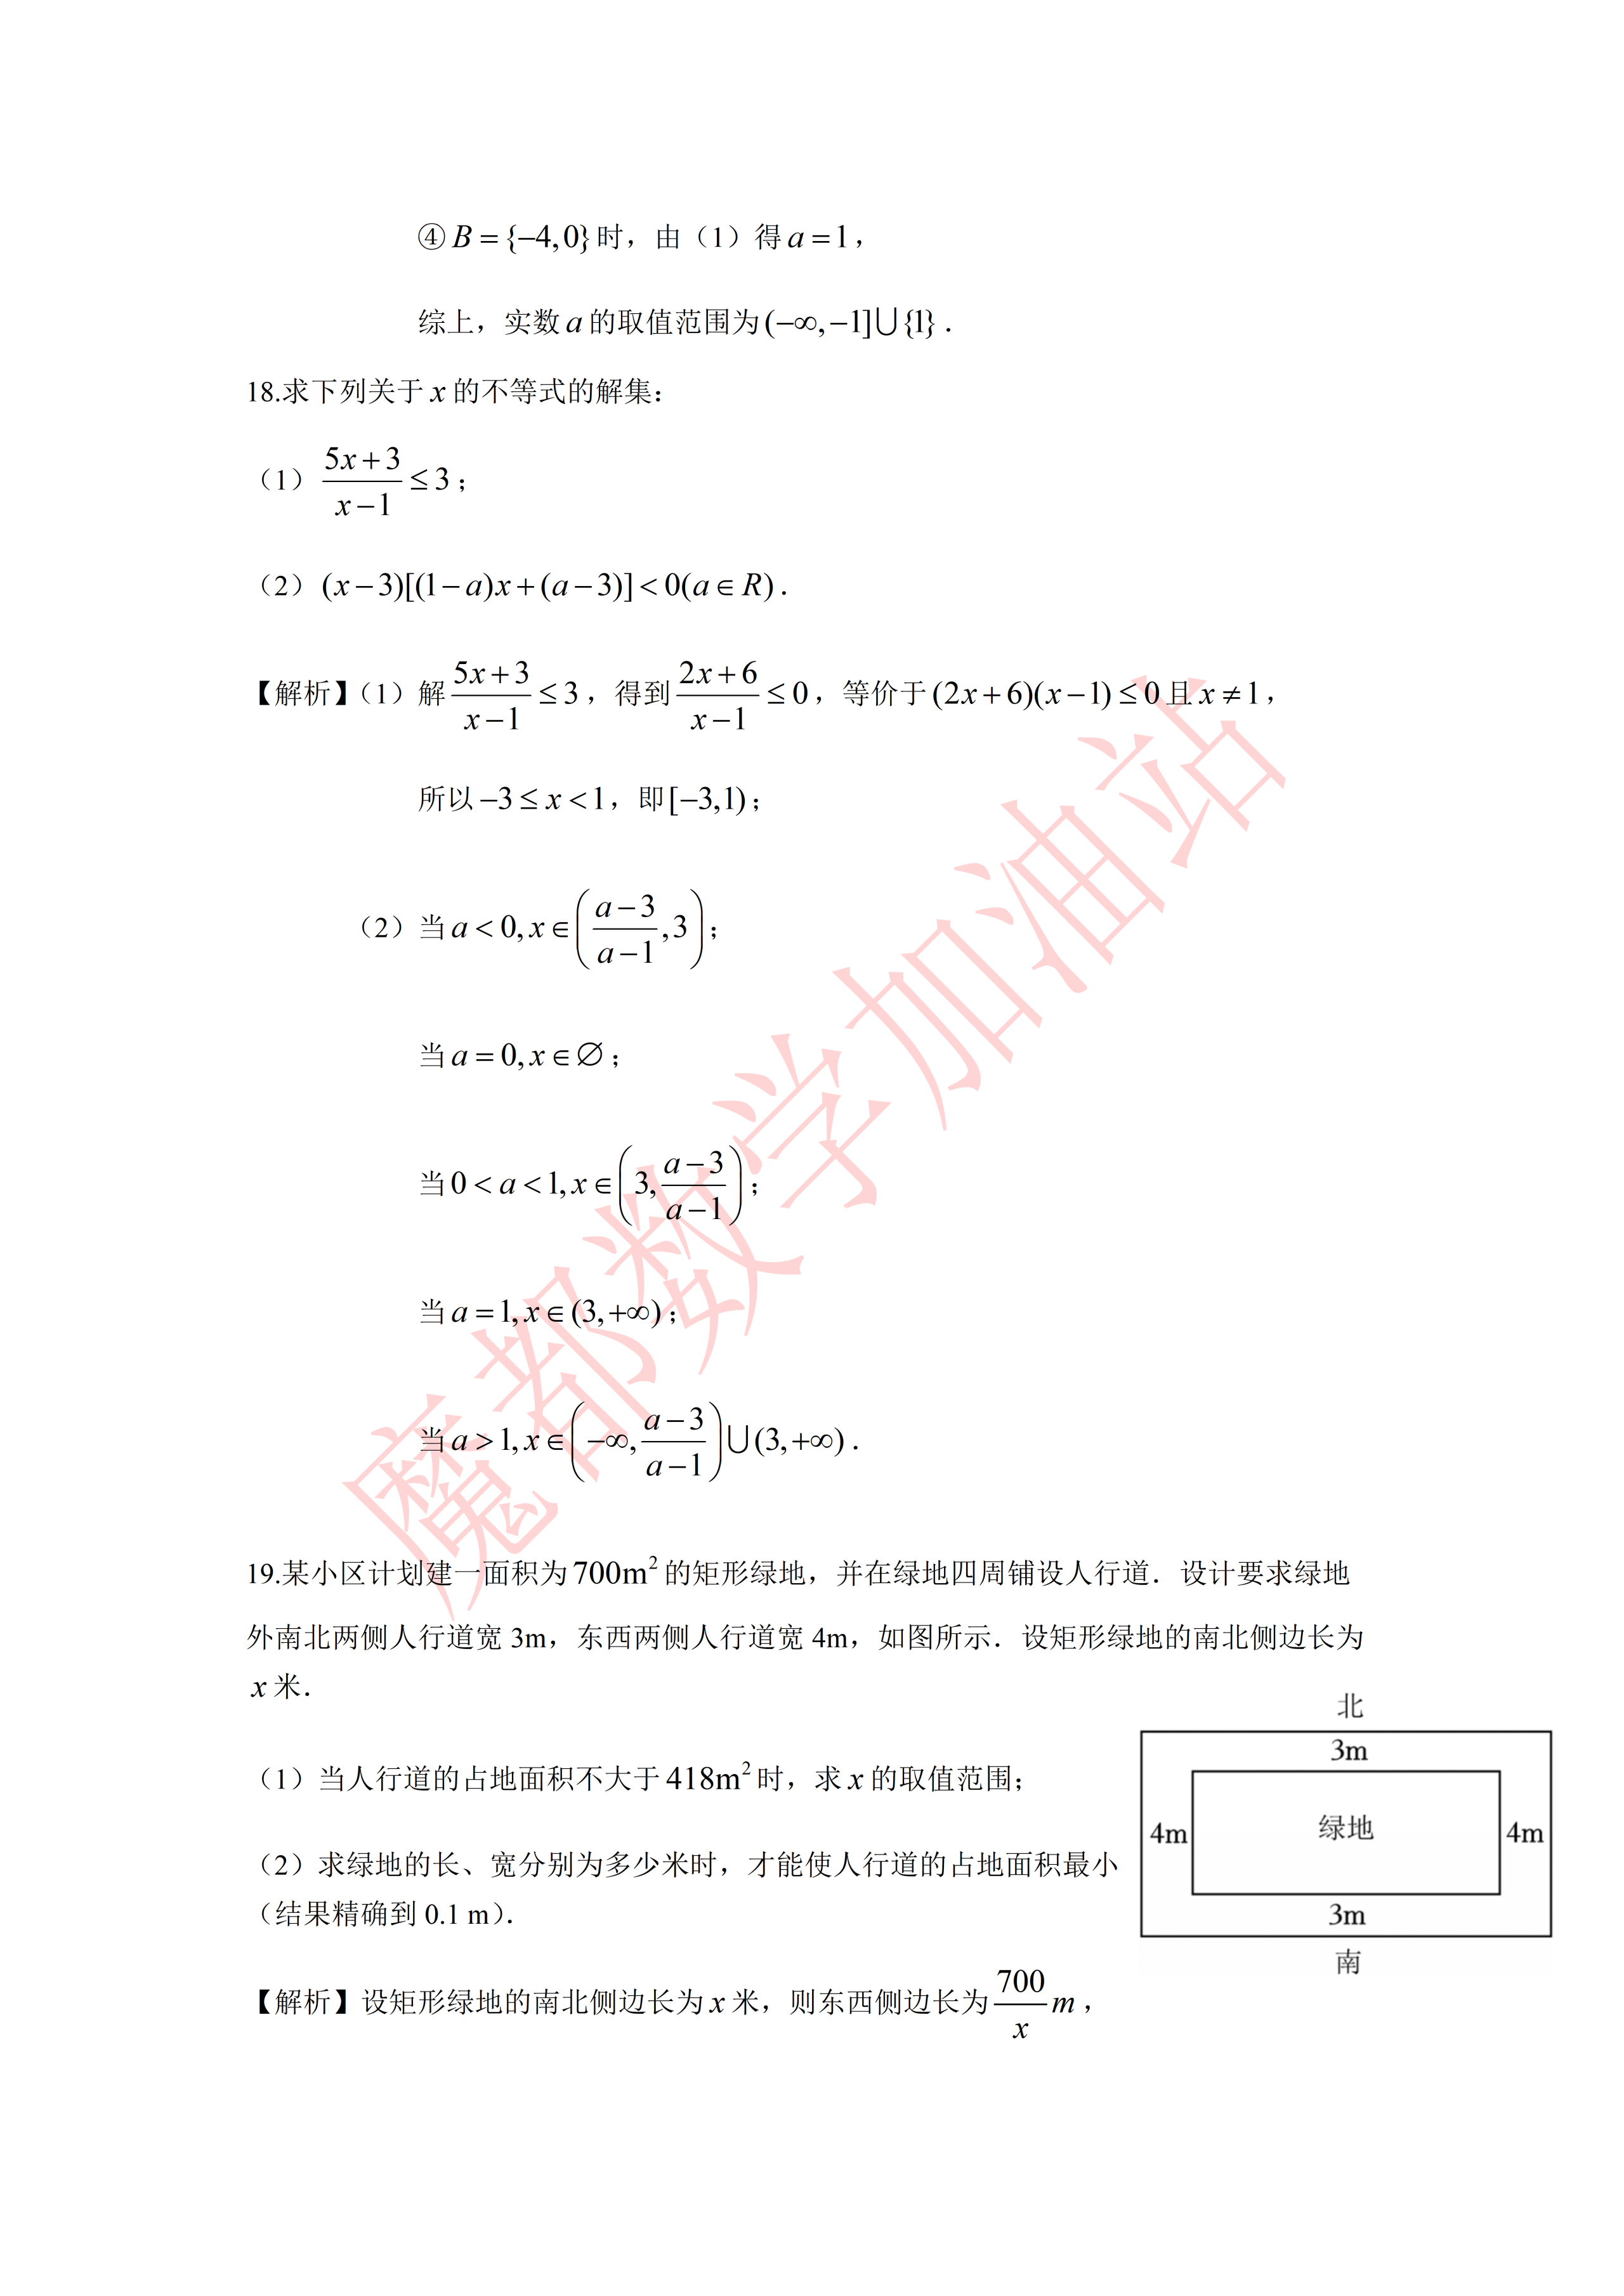
\includegraphics[width=.3\linewidth,trim=1791bp 484bp 107bp 2654bp,clip]{../原图/高一53_华师大二附中_10月月考/07.png}
\end{center}

\begin{enumerate}[label=(\arabic*)]
\item 当人行道的占地面积不大于 $418m^2$ 时，求 $x$ 的取值范围；
\item 求绿地的长、宽分别为多少米时，才能使人行道的占地面积最小（结果精确到 $0.1m$）.
\end{enumerate}

\ifanswer
\solbegin
\step{设矩形绿地的南北侧边长为 $x$ 米，则东西侧边长为 $\dfrac{700}{x}m$，}
\step{则人行道的占地面积为 $S=(x+8)\left(\dfrac{700}{x}+6\right)-700$，即 $S=6x+\dfrac{5600}{x}+48$.}
\stepm{(1)}{当人行道的占地面积不大于 $418m^2$ 时，$6x+\dfrac{5600}{x}+48\leqslant418$，}
\step{即 $6x^2-370x+5600\leqslant0$，解得 $\dfrac{80}{3}\leqslant x\leqslant35$，}
\step{故当人行道的占地面积不大于 $418m^2$ 时，$x\in\left[\dfrac{80}{3},35\right]$；}
\stepm{(2)}{$S=6x+\dfrac{5600}{x}+48\geqslant2\sqrt{6x\cdot\dfrac{5600}{x}}+48=80\sqrt{21}+48$，}
\step{当且仅当 $6x=\dfrac{5600}{x}$，即 $x=20\sqrt{\dfrac73}\approx30.6(m)$ 时，}
% 原卷如此，照录未改（80√21+48≈414.6，两处“414.4”疑笔误，见文件头“原卷笔误/存疑”第 6 条）
\step{$S$ 达到最小值 $80\sqrt{21}+48\approx414.4$，此时 $\dfrac{700}{x}\approx22.9(m)$，}
\step{所以当设计绿地的南北侧边长约为 $30.6m$，东西侧边长约为 $22.9m$ 时，}
\step{人行道的占地面积最小值为 $414.4(m^2)$.}
\solend
\fi

\ansspace[6]

\item 已知 $x\in\R$，符号 $[x]$ 表示不大于 $x$ 的最大整数，例如：$[2.3]=2$,$[2]=2$，$[-1.2]=-2$，令 $S(x)=[x]-[-x]$.

\begin{enumerate}[label=(\arabic*)]
\item 写出 $S(x)$ 为偶数（包括正、负偶数和 0）的充要条件，并证明；
\item 设方程 $|S(x)|=3$ 的解集为 $A$.

①集合 $B=\{x\mid x^2-ax-9\leqslant0,a\in\R\}$，若 $A\cap B=A$，求实数 $a$ 的取值范围；

②集合 $C=\{x\mid 2x^2-5kx+3k^2\geqslant0\}$，若 $A\cup C=\R$，求实数 $k$ 的取值范围.
\end{enumerate}

\ifanswer
\solbegin
\stepm{(1)}{$S(x)$ 为偶数的充要条件是 $x\in\Z$.}
\step{若 $x\in\Z$，则 $S(x)=[x]-[-x]=x-(-x)=2x$；}
\step{若 $x\notin\Z$，设 $[x]=n$，}
\step{则 $S(x)=[x]-[-x]=n-(-n-1)=2n+1=2[x]+1$；}
% 原卷如此，照录未改（“由①”按文意应为“由(1)”，见文件头“原卷笔误/存疑”第 3 条）
\stepm{(2)}{由①得 3 是奇数，$S(x)=\pm3$,$x\notin\Z$，}
\step{$S(x)=2[x]+1=\pm3$,$[x]=1$ 或 $-2$ 且 $x\notin\Z$，}
\step{所以 $A=(-2,-1)\cup(1,2)$；}
\stepm{①}{$A\cap B=A\Rightarrow A\subseteq B$，}
\step{设 $B=[x_1,x_2]$，其中 $x_1,x_2$ 是方程 $x^2-ax-9=0$ 的两实根，}
\step{设 $f(x)=x^2-ax-9$，}
\step{$[-2,2]\subseteq[x_1,x_2]\Leftrightarrow x_1\leqslant-2$,$x_2\geqslant2\Leftrightarrow\begin{cases}f(-2)\leqslant0\\ f(2)\leqslant0\end{cases}$}
\step{$\Leftrightarrow\begin{cases}(-2)^2-a\cdot(-2)-9\leqslant0, & a\leqslant\dfrac52\\ 2^2-2a-9\leqslant0, & a\geqslant-\dfrac52\end{cases}$，故 $a\in\left[-\dfrac52,\dfrac52\right]$；}
\step{注：若用求根公式 $\begin{cases}\dfrac{a+\sqrt{a^2+36}}{2}\geqslant2\Rightarrow a\geqslant-\dfrac52\\ \dfrac{a-\sqrt{a^2+36}}{2}\leqslant-2\Rightarrow a\leqslant\dfrac52\end{cases}$，结果正确，也得满分；}
\stepm{②}{$2x^2-5kx+3k^2=(x-k)(2x-3k)$.}
\step{$A\cup C=\R\Leftrightarrow\complement_\R A\subseteq C$.}
\step{记 $g(x)=2x^2-5kx+3k^2$，则 $\{x\mid g(x)<0\}\subseteq A$.}
\stepm{情况1：}{$k>0$ 时，$k<\dfrac32k$,$g(x)<0$ 的解集为 $\left(k,\dfrac32k\right)\subseteq(1,2)$，}
\step{故 $\begin{cases}k\geqslant1\\ \dfrac32k\leqslant2\end{cases}\Rightarrow1\leqslant k\leqslant\dfrac43$；}
\stepm{情况2：}{$k=0$ 时，$g(x)=2x^2\geqslant0$ 恒成立，$C=\R$,$A\cup C=\R$ 显然成立；}
\stepm{情况3：}{$k<0$ 时，$\dfrac32k<k$,$g(x)<0$ 的解集为 $\left(\dfrac32k,k\right)\subseteq(-2,-1)$，}
\step{故 $\begin{cases}\dfrac32k\geqslant-2\\ k\leqslant-1\end{cases}\Rightarrow-\dfrac43\leqslant k\leqslant-1$；}
\step{综上，$k\in\left[-\dfrac43,-1\right]\cup\{0\}\cup\left[1,\dfrac43\right]$.}
\solend
\fi

\ansspace[10]

\item 对于非空实数集 $M\subseteq(0,+\infty)$，若满足以下两个条件，则称 $M$ 为“极闭集”：

①$M$ 中至少含有 2 个元素，且 $1\notin M$；

②对于 $M$ 中任意两个不相等的元素 $x,y$，定义 $x*y=\dfrac{xy+1}{x+y}$，且 $x*y\in M$.

\begin{enumerate}[label=(\arabic*)]
\item 判断集合 $A=\left\{\dfrac12,2\right\}$ 与区间 $B=(1,+\infty)$ 是否为“极闭集”，并说明理由；
\item 若 $M$ 是“极闭集”，证明：集合 $M$ 中不可能所有元素都小于 1；
\item 证明：不存在任何有限的“极闭集”.
\end{enumerate}

\ifanswer
\solbegin
% 原卷如此，照录未改（首行集合按题干应为 {1/2,2}，见文件头“原卷笔误/存疑”第 7 条）
\stepm{(1)}{对于集合 $A=\left\{\dfrac12,1\right\}$，$\dfrac12*2=\dfrac45$，}
\step{因为 $\dfrac45\notin A$，不满足条件②，所以集合 $A$ 不是“极闭集”.}
\step{对于区间 $B$，满足条件①.}
\step{任取 $B$ 中两个不相等的元素 $x,y$，则 $x>1$,$y>1$.}
\step{$x*y-1=\dfrac{xy+1}{x+y}-1=\dfrac{(x-1)(y-1)}{x+y}>0$，所以 $x*y>1$，}
\step{这说明 $x*y\in B$ 恒成立，满足条件②，所以 $B$ 是“极闭集”.}
\stepm{(2)}{假设集合 $M$ 中所有元素都小于 1，}
\step{在 $M$ 中取 $0<x<y<1$,$x*y-1=\dfrac{xy+1}{x+y}-1=\dfrac{(x-1)(y-1)}{x+y}>0$，}
\step{所以 $x*y>1$，与“集合 $M$ 中所有元素都小于 1”矛盾，}
\step{假设不成立，集合 $M$ 中不可能所有元素都小于 1，得证.}
\stepm{(3)}{由②得，任何一个“极闭集”$M$ 中，必然至少存在一个大于 1 的元素，}
\stepm{情况1：}{若 $M$ 中至少存在两个大于 1 的元素，}
\step{设其中两个不相等的元素为 $x$ 和 $y_1$，且 $x>y_1>1$，}
\step{令 $y_{n+1}=x*y_n$,$n\geqslant1$,$y_{n+1}-1=x*y_n-1=\dfrac{(x-1)(y_n-1)}{xy_n+1}>0$，}
\step{如果 $y_n\geqslant1$，则显然 $y_{n+1}\geqslant1$，作差 $y_n-y_{n+1}=\dfrac{y_n^2-1}{x+y_n}>0$，}
\step{由此 $x>y_1>y_2>y_3>\cdots>1$，与有限集矛盾.}
\stepm{情况2：}{若 $M$ 中恰好只有一个元素大于 1，}
\step{设这个唯一大于 1 的元素为 $m$.}
\step{因为 $M$ 至少有两个元素，所以 $M$ 中必然至少存在一个元素 $a_1<1$，}
\step{令 $a_{n+1}=m*a_n$,$n\geqslant1$，}
\step{又 $a_{n+1}-1=m*a_n-1=\dfrac{(m-1)(a_n-1)}{m+a_n}<0$，故 $a_{n+1}<1$，}
\step{作差 $a_{n+1}-a_n=\dfrac{1-a_n^2}{m+a_n}>0$，由此 $a_1<a_2<a_3<\cdots<1$，与有限集矛盾.}
\step{因此，不存在任何有限的“极闭集”. 原命题得证.}
\solend
\fi

\ansspace*[10]

\end{enumerate}

\end{document}
"
%
% 原始材料：微信公众号“魔都数学加油站”文章，作者破晓，连载“27学年高一53”；
% 原文标题“27学年高一53——2026-2027年上海市华师大二附中高一上10月月考”；
% 原文链接：https://mp.weixin.qq.com/s/fpSnoF-gJEEWyxAoPC_bZA。
% 页面标注发布时间 2026-10-09 17:15（上海）。
% 正文为 11 张 PNG 页：第 01—06、08、10 页 4762×6735，第 07、09、11 页 2560×3620
% （**同一篇各页分辨率不同**），均按页序读取。11 页全为试卷正文页（卷首标题在第 1 页页顶，
% 卷末解答题第 21 题解析止于第 11 页），无封面页、目录页、二维码或宣传页。
% 粉色斜排“魔都数学加油站”为卷面水印，与公众号页脚一并未录入。
%
% 卷首标题：照卷面印作“2026--2027 年华师大二附中高一上 10 月月考”（公众号标题中的“上海市”
% 卷面标题行没有，本稿照卷面），年份区间按全稿惯例排 en dash。原卷只有一行标题、无副标题。
%
% 篇幅与题号：原卷自第 3 题起编号（第 1、2 题不在本卷内）。填空题 3—12（10 题）、
% 选择题 13—16（4 题）、解答题 17—21（5 题），共 19 题。本稿沿用原节与原题号，
% 只改排为全稿统一的大节样式（原卷小节标题为“一、填空题”“二、选择题”“三、解答题”）。
%
% 讲评版：原卷每题下直接印【答案】或【解析】。**第 13 题没有任何【答案】/【解析】段**，
% 答案“C”直接印在题干括号内（“一定不是(  C  )”），本稿按 高一37 第 13 题的成例把括号留空、
% 答案另提为 \ans{$C$}；其余 18 题都只印【解析】，按全稿口径这类题不另提 \ans{}——其中
% 选择题第 14、15、16 题的结论写在解析末句（“故选 B／D／C”），亦照录在解析内。
%
% 副标题：原卷未印副标题。本稿按“知识模块”口径标作“集合与常用逻辑用语、不等式”：
% 19 题中集合与常用逻辑用语 12 题（集合类 9 题——第 4、5、12、13、15、16、17、20、21 题；
% 逻辑类 3 题——第 3、9、14 题），不等式 7 题（含一元二次方程与绝对值方程：第 6、7、8、10、
% 11、18、19 题，其中第 11 题实为奇偶分析下的集合计数题，暂挂不等式），两类均超三分之一，
% 故并标。口径同 高一46、高一47、高一48、高一51、高一52。
%
% 与原卷的排版差异：
%   ① 原卷每题下直接印【解析】，本稿按全稿惯例将答案与解析置于答案版，试卷版保持干净；
%      第 13 题印在题干括号内的答案“C”同样移入 \ans{}，见上；
%   ② 原卷未印副标题，本稿按“知识模块”口径补出；
%   ③ 原卷填空横线约两个字宽，本稿按全稿惯例统一排 \blankline[4.4em]；
%      选择题的作答括号原卷排半角“(    )”，本稿按全稿惯例排 \mbox{（\quad）}；
%   ④ 原卷实数集排斜体/粗体 $R$、$\mathbf{R}$（第 4、6、7、18、20 题等处），本稿按全稿惯例
%      改用 $\R$；空集记号统一为 \varnothing；
%   ⑤ 原卷在数学式内多处用半角逗号（如 $x_1,x_2$、$|S|,|T|$、$a\neq0,c\neq0$），均照录未强改；
%      句末句点按全稿惯例排西文句点（原卷“故选 B．”一类全角句点亦从宽排作“.”）；
%   ⑥ 第 17—21 题的子问原卷各自另起一行，本稿按全稿惯例用 enumerate 的 (1)(2)(3)；
%      第 20 题 (2) 问下的①②两行是题干的一部分，照录为行首①②标号（不入 enumerate）；
%      解析中的子问标号一律用 \stepm{(1)}{…}，解析中的①②③④分情形用 \stepm{①}{…}；
%   ⑦ 第 12、20、21 题解析里的“情况1:”至“情况3:”标号原卷排**红色加粗**（全卷共 6 处），
%      全库无红色排字先例，本稿按全稿子题标号样式排 \stepm{情况1：}{…}（加粗着色、不改黑色基调），
%      冒号照原卷排全角；
%   ⑧ 第 19 题的示意图原卷排在题干右侧（与题干、(1) 问同高），本稿居中排在题干之后、
%      子问之前，并在 \item 前加 \needvspace 整块推走；图自原图第 07 页裁切（trim），不另存图片文件；
%   ⑨ 每道解答题原卷未留作答空白，本稿按全稿惯例加 \ansspace。
%
% 原卷笔误/存疑（均照录未改，正文对应处另有 % 注）：
%   1. 第 14 题解析末行“例如 $a=1$，$b=-1$，及必要性不成立”，“及”按文意应为“即”；
%   2. 第 15 题解析第 3 行 $\dfrac1{a+b\sqrt2}=\dfrac a{a^2-2b}+\left(-\dfrac b{a^2-2b}\right)\cdot\sqrt2$，
%      分母两处均作 $a^2-2b$，按通分应为 $a^2-2b^2$（结论 $C=X$ 不受影响）；
%   3. 第 20 题 (2) 问解析首行“由①得 3 是奇数”，按文意应为“由(1)得”（①是 (2) 问下自己
%      的子问标号，奇偶性结论出自 (1) 问）；
%   4. 第 11 题解析“只有奇数的有 $C_4^2+1=7$ 个”，按组合意义应为 $C_4^2+C_4^4=7$
%      （“$+1$”当指 4 个奇数全取的 1 种），数值无误；
%   5. 第 18 题 (2) 问解析“当 $a=0$,$x\in\varnothing$”，按文意应为“解集为 $\varnothing$”；
%   6. 第 19 题 (2) 问解析“$S$ 达到最小值 $80\sqrt{21}+48\approx414.4$”与末行
%      “人行道的占地面积最小值为 $414.4(m^2)$”，两处按 $80\sqrt{21}+48\approx414.6$，疑笔误；
%   7. 第 21 题 (1) 问解析首行“对于集合 $A=\left\{\frac12,1\right\}$”，按题干应为
%      $A=\left\{\frac12,2\right\}$（计算 $\frac12*2=\frac45$ 用的正是 $2$）；
%   8. 第 12 题解析“所以 $A=(-\infty,-4]\cup[2,+\infty)$”一行行末无标点，体例不一，照录。
%
% 插图：1 张，自原图裁切（无 \begin{tikzpicture} 重排）：
%   · 第 19 题绿地示意图（外矩形内套矩形“绿地”，上“北 3m”、下“南 3m”、左右各“4m”）
%     ——原图第 07 页，原卷排于题干右侧。
%     裁框：x 1797–2447、y 2660–3136（含“北”“南”标注，四周各留约 6px），
%     trim=1791bp 484bp 107bp 2654bp（左／下／右／上），页宽 2560、页高 3620。
%
\documentclass[a4paper,11pt]{article}
\usepackage{common}

\begin{document}

\examtitlest[3]{2026--2027 年华师大二附中高一上 10 月月考}{集合与常用逻辑用语、不等式}

\bigsec{一、填空题}

\begin{enumerate}
\setcounter{enumi}{2}

\item “$x=2$”是“$x^2-3x+2=0$”的\blankline[4.4em]条件.

（选择其中之一填空：充分非必要、必要非充分、充分、既非充分又非必要）

\ifanswer
\solbegin
\step{由 $x^2-3x+2=0$ 得 $x=1$ 或 $x=2$，}
\step{则“$x=2$”是“$x^2-3x+2=0$”的充分不必要条件.}
\solend
\fi

\item 已知 $R$ 是全集，集合 $A=\{y\mid y=-x^2+1,x\in\R\}$，集合 $B=\{x\mid x=3+|a|,a\in\R\}$，则 $\overline{A\cup B}=$\blankline[4.4em].

\ifanswer
\solbegin
\step{$A=\{y\mid y=-x^2+1,x\in\R\}=(-\infty,1]$，$B=\{x\mid x=3+|a|,a\in\R\}=[3,+\infty)$，}
\step{所以 $\overline{A\cup B}=(1,3)$.}
\solend
\fi

\item 已知 $a$ 为常数，集合 $A=\{x\mid x^2+x-6=0\}$，集合 $B=\{x\mid ax-2=0\}$，且 $B\subseteq A$，则 $a$ 的所有取值构成的集合为\blankline[4.4em].

\ifanswer
\solbegin
\step{集合 $A=\{-3,2\}$，因为 $B\subseteq A$，则 $B=\varnothing$，$\{-3\}$，$\{2\}$，$\{-3,2\}$，}
\step{当 $B=\varnothing$ 时，$a=0$，当 $B=\{-3\}$ 时，$a=-\dfrac23$，当 $B=\{2\}$ 时，$a=1$，}
\step{当 $B=\{-3,2\}$ 时，不成立，故 $a$ 的取值集合为 $\left\{0,-\dfrac23,1\right\}$.}
\solend
\fi

\item 设 $a\in\R$，若关于 $x$ 的不等式 $x^2-ax<0$ 的解集是区间 $(0,1)$ 的真子集，则 $a$ 的取值范围是\blankline[4.4em].

\ifanswer
\solbegin
\step{因为关于 $x$ 的不等式 $x^2-ax<0$ 的解集是区间 $(0,1)$ 的真子集，}
\step{当 $a=0$ 时，不等式的解集为 $\varnothing$，符合题意；}
\step{当 $a>0$ 时，不等式的解集为 $(0,a)$，则 $0<a<1$，}
\step{当 $a<0$ 时，不等式的解集为 $(a,0)$，不符合题意，}
\step{故 $a$ 的范围为 $[0,1)$.}
\solend
\fi

\item 设 $x\in\R$，则方程 $|2x+3|-|x-2|=|3x+1|$ 的解集为\blankline[4.4em].

\ifanswer
\solbegin
\step{当 $x\leqslant-\dfrac32$ 时，原式$\Leftrightarrow-2x-3+x-2=-3x-1\Leftrightarrow x=2$，不合题意；}
\step{当 $-\dfrac32<x\leqslant-\dfrac13$ 时，原式$\Leftrightarrow2x+3+x-2=-3x-1\Leftrightarrow x=-\dfrac13$；}
\step{当 $-\dfrac13<x\leqslant2$ 时，原式$\Leftrightarrow2x+3+x-2=3x+1\Leftrightarrow1=1$ 即恒成立；}
\step{当 $x>2$ 时，原式$\Leftrightarrow2x+3+2-x=3x+1\Leftrightarrow x=2$，不合题意；}
\step{故 $x\in\left[-\dfrac13,2\right]$.}
\solend
\fi

\item 已知关于 $x$ 的一元二次方程 $x^2+(4m+1)x+2m-1=0$．若方程的两根为 $x_1$、$x_2$，且满足 $\dfrac1{x_1}+\dfrac1{x_2}=-\dfrac12$，则实数 $m=$\blankline[4.4em].

\ifanswer
\solbegin
\step{由于判别式$\Delta=16m^2+5>0$恒成立，}
\step{不论 $m$ 为任何实数，方程总有两个不相等的实数根.}
\step{$\dfrac1{x_1}+\dfrac1{x_2}=-\dfrac12$，即 $\dfrac{x_1+x_2}{x_1x_2}=-\dfrac12$，由根与系数的关系得 $\dfrac{-4m-1}{2m-1}=-\dfrac12$，}
\step{解得 $m=-\dfrac12$.}
\solend
\fi

\item 已知 $\dfrac1{x-2}\geqslant1$ 是 $|x-a|<2$ 的充分非必要条件，则实数 $a$ 的取值范围是\blankline[4.4em].

\ifanswer
\solbegin
\step{由 $\dfrac1{x-2}\geqslant1$ 得 $\dfrac{3-x}{x-2}\geqslant0$，解得 $2<x\leqslant3$，由 $|x-a|<2$ 得 $a-2<x<a+2$，}
\step{因为 $\dfrac1{x-2}\geqslant1$ 是 $|x-a|<2$ 的充分非必要条件，}
\step{所以 $\{x\mid 2<x\leqslant3\}\subset\{x\mid a-2<x<a+2\}$，所以 $\begin{cases}a-2\leqslant2\\ a+2>3\end{cases}$，解得 $1<a\leqslant4$，}
\step{即实数 $a$ 的取值范围是 $(1,4]$.}
\solend
\fi

\item 设 $x,y\in(0,+\infty)$，且 $x+4y=1$，则 $\dfrac1x+\dfrac1y$ 的最小值为\blankline[4.4em].

\ifanswer
\solbegin
\step{因为 $\dfrac1x+\dfrac1y=(x+4y)\left(\dfrac1x+\dfrac1y\right)=5+\dfrac{4y}{x}+\dfrac{x}{y}\geqslant5+2\sqrt{\dfrac{4y}{x}\cdot\dfrac{x}{y}}=9$，}
\step{当且仅当 $\dfrac{4y}{x}=\dfrac{x}{y}$，即 $x=2y$，即 $x=\dfrac13$,$y=\dfrac16$ 时取等号，故最小值为 $9$.}
\solend
\fi

\item 设非空集合 $Q\subseteq M$，当 $Q$ 中所有元素和为偶数时（集合为单元素时和为元素本身），称 $Q$ 是 $M$ 的偶子集. 若集合 $M=\{1,2,3,4,5,6,7\}$，则其偶子集 $Q$ 的个数为\blankline[4.4em].

\ifanswer
\solbegin
\step{偶子集可以分为只有奇数、偶数及偶数个奇数和偶数的集合，}
\step{奇数有 4 个，偶数有 3 个，}
% 原卷如此，照录未改：按组合意义应为 C_4^2+C_4^4=7（“+1”当指 4 个奇数全取的 1 种），
% 见文件头“原卷笔误/存疑”第 4 条
\step{只有奇数的有 $C_4^2+1=7$ 个，只有偶数的有 $C_3^1+C_3^2+1=7$ 个，}
\step{偶数个奇数和偶数的：两奇一偶 $C_4^2\cdot C_3^1=18$ 个，两奇二偶 $C_4^2\cdot C_3^2=18$ 个，}
\step{两奇三偶 $C_4^2\cdot C_3^3=6$ 个，四奇一偶 $C_4^4\cdot C_3^1=3$ 个，四奇二偶 $C_4^4\cdot C_3^2=3$ 个，}
\step{四奇三偶 $C_4^4\cdot C_3^3=1$ 个，所以共有 $7+7+18+18+6+3+3+1=63$ 个.}
\solend
\fi

\item 已知集合 $A=\{x\mid x^2+2x-8\geqslant0\}$,$B=\{x\mid x^2-2ax+2a\leqslant0\}$，且 $A\cap B$ 中恰有 3 个整数元素，则实数 $a$ 的取值范围为\blankline[4.4em].

\ifanswer
\solbegin
% 原卷如此，照录未改：此行行末无标点，见文件头“原卷笔误/存疑”第 8 条
\step{由 $x^2+2x-8\geqslant0$，得 $x\geqslant2$ 或 $x\leqslant-4$，所以 $A=(-\infty,-4]\cup[2,+\infty)$}
\step{对集合 $B$：$x^2-2ax+2a\leqslant0$,$\Delta=4a^2-8a=4a(a-2)\geqslant0$，}
\step{得 $a\leqslant0$ 或 $a\geqslant2$.}
\step{设方程 $x^2-2ax+2a=0$ 的两根为 $r_1,r_2$，}
\step{则 $B=[r_1,r_2]$,$r_1=a-\sqrt{a^2-2a}$,$r_2=a+\sqrt{a^2-2a}$，}
\stepm{情况1：}{$a\leqslant0$，}
\step{$r_2=a+\sqrt{a^2-2a}<a+\sqrt{a^2-2a+1}=a+|a-1|=a+1-a=1<2$，}
\step{$B$ 只在 $A$ 的左侧部分有交集，要使 $A\cap B$ 恰有 3 个整数元素，}
\step{这 3 个整数为 $-6,-5,-4$，于是 $r_1\in(-7,-6]$，}
\step{令 $f(x)=x^2-2ax+2a$，则 $\begin{cases}f(-7)=49+14a+2a>0\\ f(-6)=36+12a+2a\leqslant0\end{cases}\Rightarrow a\in\left(-\dfrac{49}{16},-\dfrac{18}{7}\right]$；}
\stepm{情况2：}{$a\geqslant2$，}
\step{$r_2=a+\sqrt{a^2-2a}\geqslant2$，}
\step{$r_1=a-\sqrt{a^2-2a}>a-\sqrt{a^2-2a+1}=a-|a-1|=a-(a-1)=1>-4$，}
\step{所以 $A\cap B=[2,r_2]$.}
\step{同理 $\begin{cases}f(4)=16-8a+2a\leqslant0\\ f(5)=25-10a+2a>0\end{cases}\Rightarrow a\in\left[\dfrac{8}{3},\dfrac{25}{8}\right)$；}
\step{综上，$a\in\left(-\dfrac{49}{16},-\dfrac{18}{7}\right]\cup\left[\dfrac{8}{3},\dfrac{25}{8}\right)$.}
\solend
\fi

\end{enumerate}

\bigsec{二、选择题}

\begin{enumerate}
\setcounter{enumi}{12}

% 第 13 题原卷无【答案】/【解析】段，答案“C”直接印在题干括号内，
% 按高一37 第 13 题的成例括号留空、答案另提为 \ans{}（见文件头）
\item 集合 $A=\{a,b,c\}$ 中的三个元素分别表示某一个三角形的三边长度，那么这个三角形一定不是\mbox{（\quad）}

\keepwithprev
A. 锐角三角形\qquad B. 钝角三角形

C. 等腰三角形\qquad D. 直角三角形

\ifanswer
\ans{$C$}
\fi

\item 设 $a$、$b$ 为实数，则“$a<b<0$”是“$\dfrac1a>\dfrac1b$”的\mbox{（\quad）}条件.

\keepwithprev
A. 充要\qquad B. 充分不必要

C. 必要不充分\qquad D. 既不充分也不必要

\ifanswer
\solbegin
\step{若 $a<b<0$，则 $\dfrac1a>\dfrac1b$ 一定成立，即充分性成立；}
% 原卷如此，照录未改（“及”按文意应为“即”，见文件头“原卷笔误/存疑”第 1 条）
\step{若 $\dfrac1a>\dfrac1b$ 成立，$a<b<0$ 不一定成立，例如 $a=1$，$b=-1$，及必要性不成立.}
\step{故选 $B$.}
\solend
\fi

\item 设 $Q$ 表示有理数集，集合 $X=\{x\mid x=a+b\sqrt2,a,b\in Q,x\neq0\}$，在下列集合中：①$\{2x\mid x\in X\}$②$\left\{\dfrac{x}{\sqrt2}\mid x\in X\right\}$③$\left\{\dfrac1x\mid x\in X\right\}$④$\{x^2\mid x\in X\}$，与 $X$ 相同的集合有\mbox{（\quad）}

\keepwithprev
A. ①②③④\qquad B. ②③④\qquad C. ①②④\qquad D. ①②③

\ifanswer
\solbegin
\step{$A=\{2x\mid x\in X\}$，$2(a+b\sqrt2)=p+q\sqrt2$ 得 $p=2a$，$q=2b$，$a=\dfrac p2$，$b=\dfrac q2$，}
\step{也是一一对应，$A=X$}
% 原卷如此，照录未改：分母两处均作 a^2-2b，按通分应为 a^2-2b^2，
% 见文件头“原卷笔误/存疑”第 2 条
\step{集合 $B=\left\{\dfrac{x}{\sqrt2}\mid x\in X\right\}$，$\dfrac{a+b\sqrt2}{\sqrt2}=b+\dfrac a2\cdot\sqrt2$，也是一一对应，$B=X$}
\step{集合 $C=\left\{\dfrac1x\mid x\in X\right\}$，$\dfrac{1}{a+b\sqrt2}=\dfrac{a}{a^2-2b}+\left(-\dfrac{b}{a^2-2b}\right)\cdot\sqrt2$，一一对应，$C=X$}
\step{集合 $D=\{x^2\mid x\in X\}$，$(a+b\sqrt2)^2=a^2+2b^2+2ab\sqrt2$，这个不能一一对应了，}
\step{集合 $D$ 包含于 $X$ 中.}
\step{故 $X$ 相同的集合有①②③，故选 $D$.}
\solend
\fi

\item 集合 $S=\{x\mid(x+a)(x^2+bx+c)=0\}$,$T=\{x\mid(ax+1)(cx^2+bx+1)=0\}$，其中 $a,b,c$ 为实数，若 $|S|,|T|$ 分别表示集合 $S,T$ 的元素个数，则 $|S|-|T|$ 的所有可能取值集合为\mbox{（\quad）}

\keepwithprev
A. $\{0\}$\qquad B. $\{1\}$\qquad C. $\{0,1\}$\qquad D. $\{-1,0,1\}$

\ifanswer
\solbegin
\stepm{①}{$a\neq0,c\neq0$ 时.}
\step{$S$ 中 $x+a=0$ 的根 $x=-a$;$T$ 中 $ax+1=0$ 的根 $x=-\dfrac1a$.}
\step{$S$ 中的 $x^2+bx+c=0$ 若无实根，则 $T$ 中的 $cx^2+bx+1=0$ 也无实根；}
\step{又设 $S$ 的 $x^2+bx+c=0$ 的根为 $r(r\neq0)$，则 $T$ 的 $cx^2+bx+1=0$ 的根为 $\dfrac1r$.}
\step{（因为 $r^2+br+c=0\Rightarrow c\cdot\left(\dfrac1r\right)^2+b\cdot\dfrac1r+1=0$）}
\step{即 $a\neq0,c\neq0$ 时，}
\step{$S$ 与 $T$ 的实根存在一一对应关系 $x\leftrightarrow\dfrac1x$,$|S|=|T|,$$|S|-|T|=0$；}
\stepm{②}{$a=0,c\neq0$ 时.}
\step{$S$ 中多出一个根 $x=0$，而 $T$ 中无此根，$|S|=|T|+1$，即 $|S|-|T|=1$；}
\stepm{③}{$a\neq0,c=0$ 时.}
\step{则 $S$ 中仍有根 $x=0$，而 $T$ 中无 0 根，同样 $|S|-|T|=1$.}
\stepm{④}{$a=0,c=0$ 时.}
\step{同样 $S$ 含有根 0，而 $T$ 中不含 0，仍有 $|S|-|T|=1$.}
\step{综上，$|S|-|T|$ 所有可能取值为 0 和 1，故选 $C$.}
\solend
\fi

\end{enumerate}

\bigsec{三、解答题}

\begin{enumerate}
\setcounter{enumi}{16}

\item 已知集合 $A=\{x\mid x^2+4x=0\}$，$B=\{x\mid x^2+2(a+1)x+a^2-1=0\}$.

\begin{enumerate}[label=(\arabic*)]
\item 若 $A$ 是 $B$ 的子集，求实数 $a$ 的值；
\item 若 $B$ 是 $A$ 的子集，求实数 $a$ 的取值范围.
\end{enumerate}

\ifanswer
\solbegin
\stepm{(1)}{因为 $A=\{-4,0\}$，$B=\{x\mid x^2+2(a+1)x+a^2-1=0\}$，又 $A\subseteq B$，}
\step{所以 $A=B$，所以 $\begin{cases}-4+0=-2(a+1)\\ -4\times0=a^2-1\end{cases}$，所以 $a=1$；}
\stepm{(2)}{因为 $B$ 是 $A$ 的子集，所以 $B=\varnothing$ 或 $B=\{-4\}$ 或 $B=\{0\}$ 或 $B=\{-4,0\}$，}
\stepm{①}{$B=\varnothing$ 时，$\Delta=4(a+1)^2-4(a^2-1)<0$，所以 $a<-1$；}
\stepm{②}{$B=\{-4\}$ 时，$\begin{cases}-4+(-4)=-2(a+1)\\ -4\times(-4)=a^2-1\end{cases}$，无解；}
\stepm{③}{$B=\{0\}$ 时，$\begin{cases}0+0=-2(a+1)\\ 0\times0=a^2-1\end{cases}$，所以 $a=-1$；}
\stepm{④}{$B=\{-4,0\}$ 时，由（1）得 $a=1$，}
\step{综上，实数 $a$ 的取值范围为 $(-\infty,-1]\cup\{1\}$.}
\solend
\fi

\ansspace[6]

\item 求下列关于 $x$ 的不等式的解集：

\begin{enumerate}[label=(\arabic*)]
\item $\dfrac{5x+3}{x-1}\leqslant3$；
\item $(x-3)[(1-a)x+(a-3)]<0$ ($a\in\R$).
\end{enumerate}

\ifanswer
\solbegin
\stepm{(1)}{解 $\dfrac{5x+3}{x-1}\leqslant3$，得到 $\dfrac{2x+6}{x-1}\leqslant0$，等价于 $(2x+6)(x-1)\leqslant0$ 且 $x\neq1$，}
\step{所以 $-3\leqslant x<1$，即 $[-3,1)$；}
\stepm{(2)}{当 $a<0$,$x\in\left(\dfrac{a-3}{a-1},3\right)$；}
% 原卷如此，照录未改（“x∈∅”按文意应为“解集为 ∅”，见文件头“原卷笔误/存疑”第 5 条）
\step{当 $a=0$,$x\in\varnothing$；}
\step{当 $0<a<1$,$x\in\left(3,\dfrac{a-3}{a-1}\right)$；}
\step{当 $a=1$,$x\in(3,+\infty)$；}
\step{当 $a>1$,$x\in\left(-\infty,\dfrac{a-3}{a-1}\right)\cup(3,+\infty)$.}
\solend
\fi

\ansspace[6]

\needvspace{13\baselineskip}

\item 某小区计划建一面积为 $700m^2$ 的矩形绿地，并在绿地四周铺设人行道. 设计要求绿地外南北两侧人行道宽 $3m$，东西两侧人行道宽 $4m$，如图所示. 设矩形绿地的南北侧边长为 $x$ 米.

\begin{center}
% 原图第 7 页题干绿地示意图直接裁取（原卷排于题干右侧）。
% 裁框取图形外框 x 1797–2447、y 2660–3136（含“北”“南”标注，四周各留约 6px），
% trim=左 1791bp／下 484bp／右 107bp／上 2654bp（页宽 2560、页高 3620）。
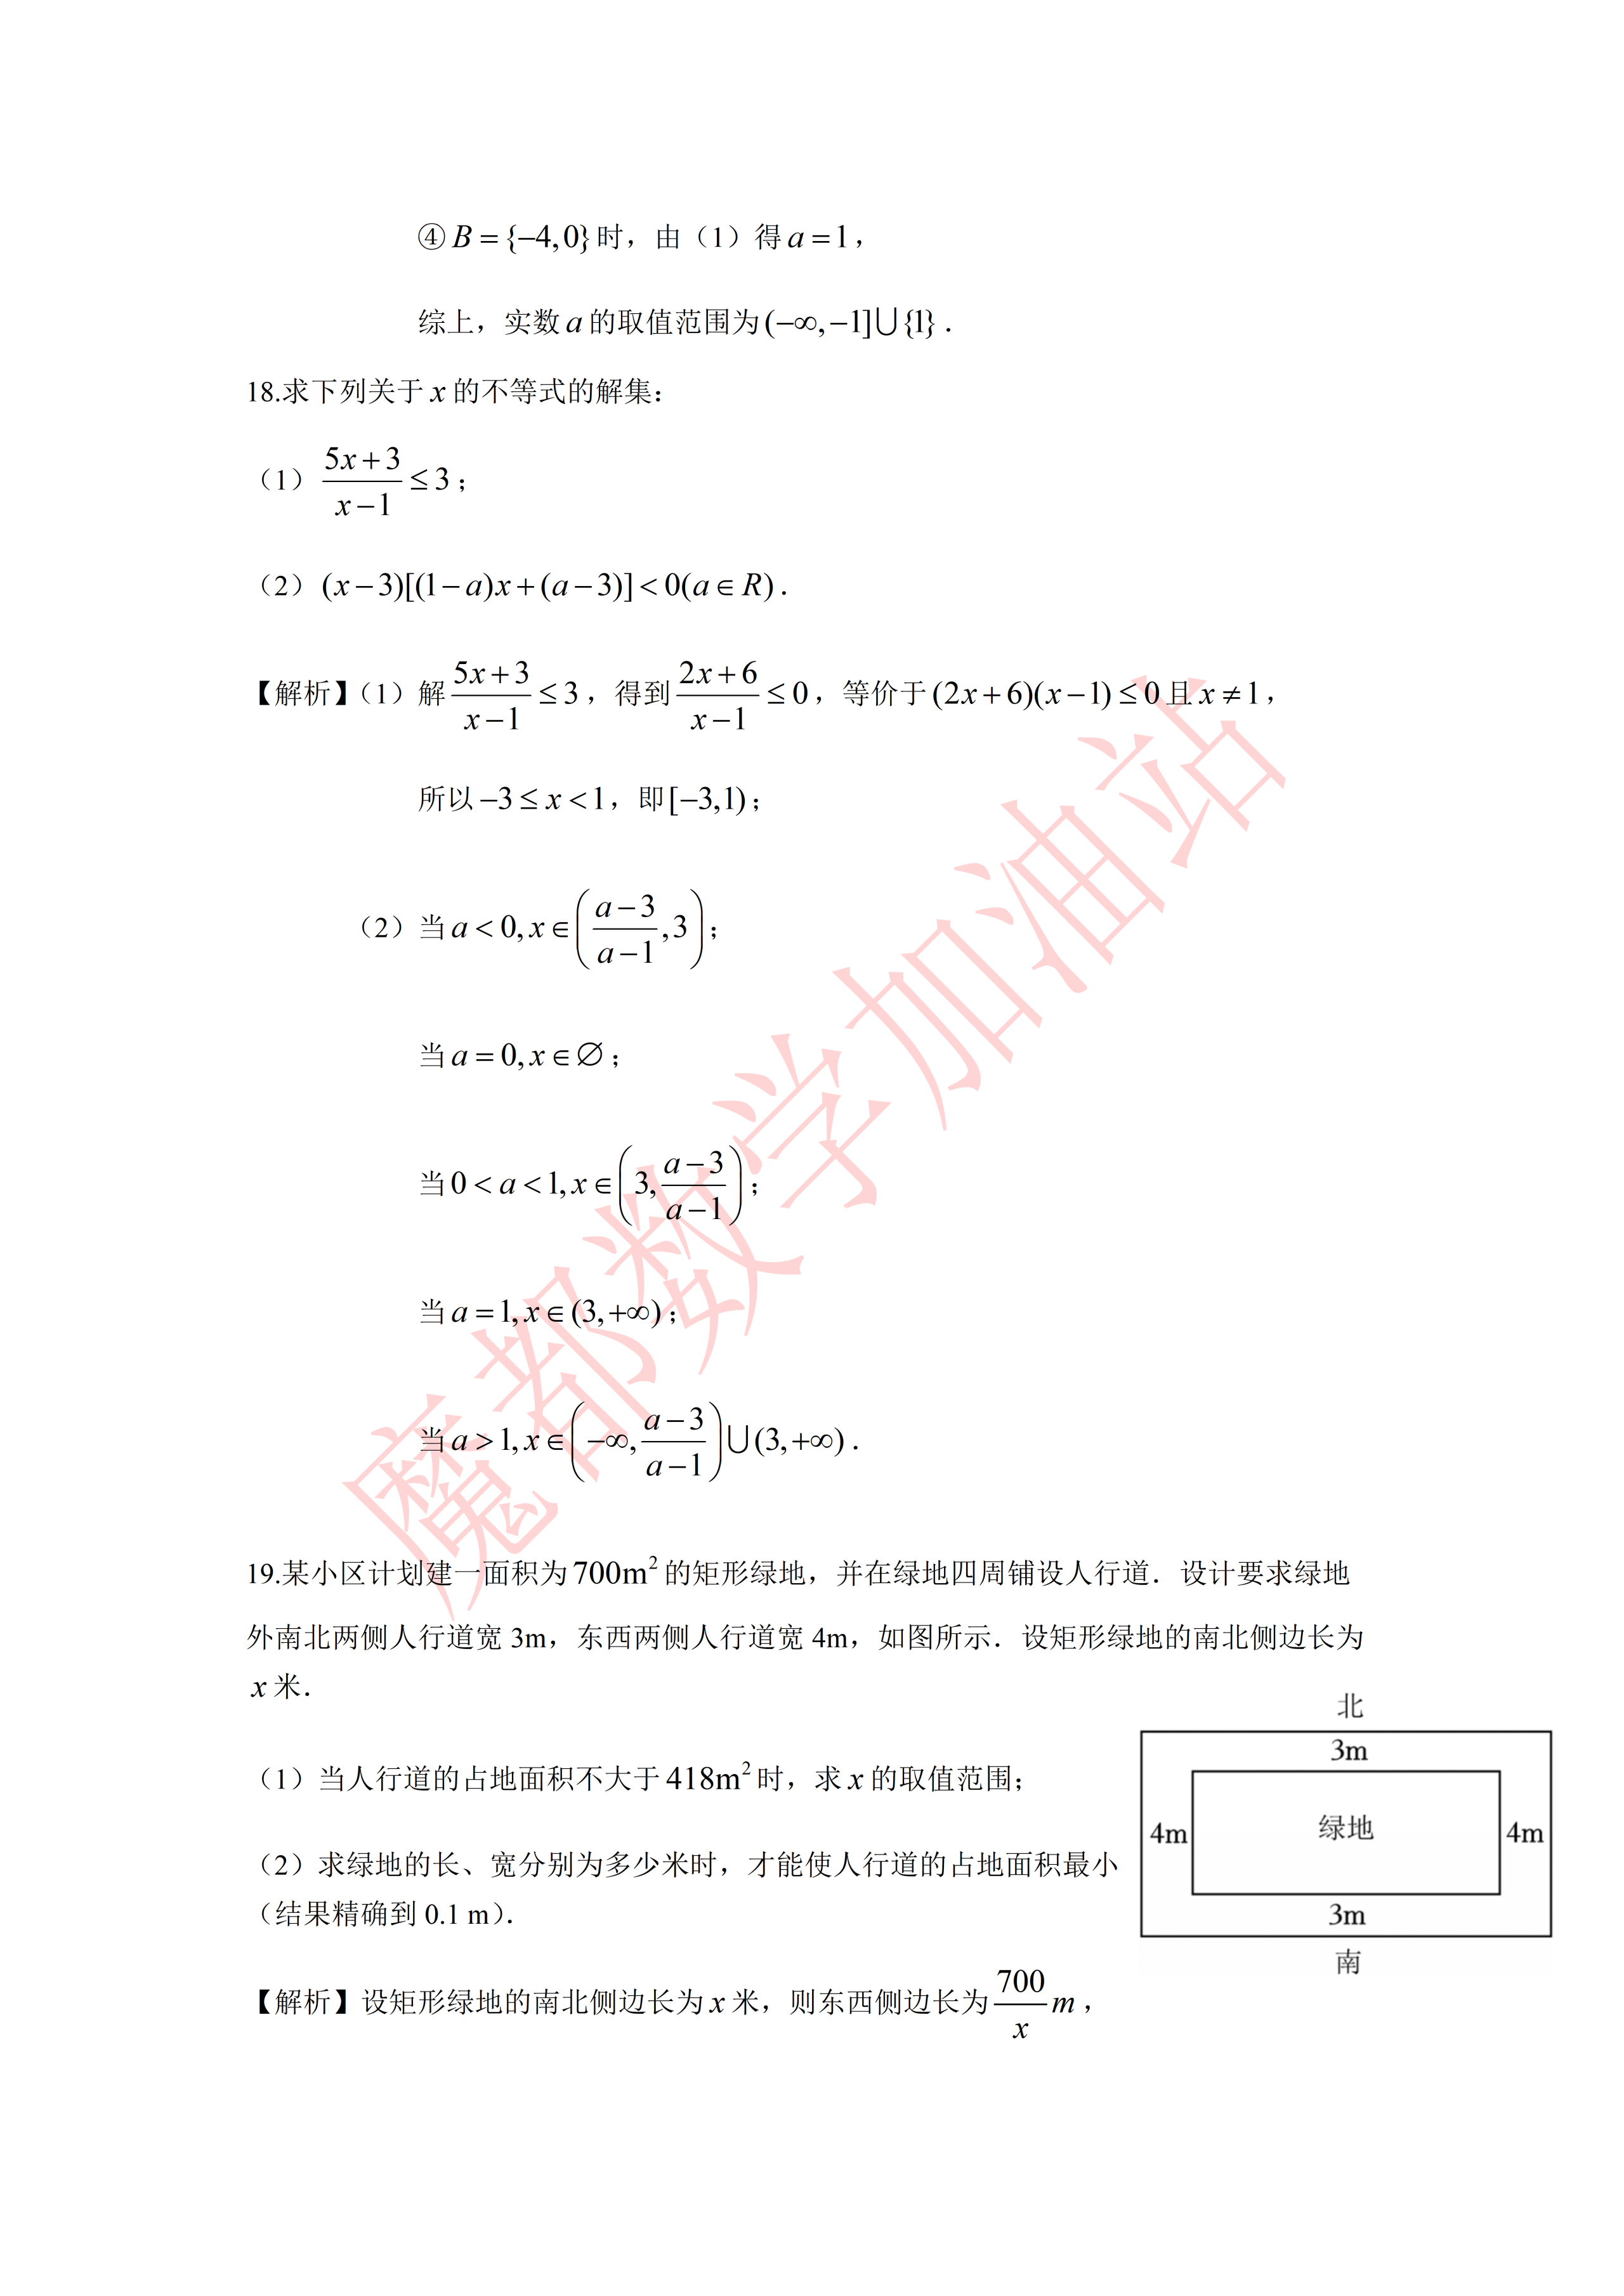
\includegraphics[width=.3\linewidth,trim=1791bp 484bp 107bp 2654bp,clip]{../原图/高一53_华师大二附中_10月月考/07.png}
\end{center}

\begin{enumerate}[label=(\arabic*)]
\item 当人行道的占地面积不大于 $418m^2$ 时，求 $x$ 的取值范围；
\item 求绿地的长、宽分别为多少米时，才能使人行道的占地面积最小（结果精确到 $0.1m$）.
\end{enumerate}

\ifanswer
\solbegin
\step{设矩形绿地的南北侧边长为 $x$ 米，则东西侧边长为 $\dfrac{700}{x}m$，}
\step{则人行道的占地面积为 $S=(x+8)\left(\dfrac{700}{x}+6\right)-700$，即 $S=6x+\dfrac{5600}{x}+48$.}
\stepm{(1)}{当人行道的占地面积不大于 $418m^2$ 时，$6x+\dfrac{5600}{x}+48\leqslant418$，}
\step{即 $6x^2-370x+5600\leqslant0$，解得 $\dfrac{80}{3}\leqslant x\leqslant35$，}
\step{故当人行道的占地面积不大于 $418m^2$ 时，$x\in\left[\dfrac{80}{3},35\right]$；}
\stepm{(2)}{$S=6x+\dfrac{5600}{x}+48\geqslant2\sqrt{6x\cdot\dfrac{5600}{x}}+48=80\sqrt{21}+48$，}
\step{当且仅当 $6x=\dfrac{5600}{x}$，即 $x=20\sqrt{\dfrac73}\approx30.6(m)$ 时，}
% 原卷如此，照录未改（80√21+48≈414.6，两处“414.4”疑笔误，见文件头“原卷笔误/存疑”第 6 条）
\step{$S$ 达到最小值 $80\sqrt{21}+48\approx414.4$，此时 $\dfrac{700}{x}\approx22.9(m)$，}
\step{所以当设计绿地的南北侧边长约为 $30.6m$，东西侧边长约为 $22.9m$ 时，}
\step{人行道的占地面积最小值为 $414.4(m^2)$.}
\solend
\fi

\ansspace[6]

\item 已知 $x\in\R$，符号 $[x]$ 表示不大于 $x$ 的最大整数，例如：$[2.3]=2$,$[2]=2$，$[-1.2]=-2$，令 $S(x)=[x]-[-x]$.

\begin{enumerate}[label=(\arabic*)]
\item 写出 $S(x)$ 为偶数（包括正、负偶数和 0）的充要条件，并证明；
\item 设方程 $|S(x)|=3$ 的解集为 $A$.

①集合 $B=\{x\mid x^2-ax-9\leqslant0,a\in\R\}$，若 $A\cap B=A$，求实数 $a$ 的取值范围；

②集合 $C=\{x\mid 2x^2-5kx+3k^2\geqslant0\}$，若 $A\cup C=\R$，求实数 $k$ 的取值范围.
\end{enumerate}

\ifanswer
\solbegin
\stepm{(1)}{$S(x)$ 为偶数的充要条件是 $x\in\Z$.}
\step{若 $x\in\Z$，则 $S(x)=[x]-[-x]=x-(-x)=2x$；}
\step{若 $x\notin\Z$，设 $[x]=n$，}
\step{则 $S(x)=[x]-[-x]=n-(-n-1)=2n+1=2[x]+1$；}
% 原卷如此，照录未改（“由①”按文意应为“由(1)”，见文件头“原卷笔误/存疑”第 3 条）
\stepm{(2)}{由①得 3 是奇数，$S(x)=\pm3$,$x\notin\Z$，}
\step{$S(x)=2[x]+1=\pm3$,$[x]=1$ 或 $-2$ 且 $x\notin\Z$，}
\step{所以 $A=(-2,-1)\cup(1,2)$；}
\stepm{①}{$A\cap B=A\Rightarrow A\subseteq B$，}
\step{设 $B=[x_1,x_2]$，其中 $x_1,x_2$ 是方程 $x^2-ax-9=0$ 的两实根，}
\step{设 $f(x)=x^2-ax-9$，}
\step{$[-2,2]\subseteq[x_1,x_2]\Leftrightarrow x_1\leqslant-2$,$x_2\geqslant2\Leftrightarrow\begin{cases}f(-2)\leqslant0\\ f(2)\leqslant0\end{cases}$}
\step{$\Leftrightarrow\begin{cases}(-2)^2-a\cdot(-2)-9\leqslant0, & a\leqslant\dfrac52\\ 2^2-2a-9\leqslant0, & a\geqslant-\dfrac52\end{cases}$，故 $a\in\left[-\dfrac52,\dfrac52\right]$；}
\step{注：若用求根公式 $\begin{cases}\dfrac{a+\sqrt{a^2+36}}{2}\geqslant2\Rightarrow a\geqslant-\dfrac52\\ \dfrac{a-\sqrt{a^2+36}}{2}\leqslant-2\Rightarrow a\leqslant\dfrac52\end{cases}$，结果正确，也得满分；}
\stepm{②}{$2x^2-5kx+3k^2=(x-k)(2x-3k)$.}
\step{$A\cup C=\R\Leftrightarrow\complement_\R A\subseteq C$.}
\step{记 $g(x)=2x^2-5kx+3k^2$，则 $\{x\mid g(x)<0\}\subseteq A$.}
\stepm{情况1：}{$k>0$ 时，$k<\dfrac32k$,$g(x)<0$ 的解集为 $\left(k,\dfrac32k\right)\subseteq(1,2)$，}
\step{故 $\begin{cases}k\geqslant1\\ \dfrac32k\leqslant2\end{cases}\Rightarrow1\leqslant k\leqslant\dfrac43$；}
\stepm{情况2：}{$k=0$ 时，$g(x)=2x^2\geqslant0$ 恒成立，$C=\R$,$A\cup C=\R$ 显然成立；}
\stepm{情况3：}{$k<0$ 时，$\dfrac32k<k$,$g(x)<0$ 的解集为 $\left(\dfrac32k,k\right)\subseteq(-2,-1)$，}
\step{故 $\begin{cases}\dfrac32k\geqslant-2\\ k\leqslant-1\end{cases}\Rightarrow-\dfrac43\leqslant k\leqslant-1$；}
\step{综上，$k\in\left[-\dfrac43,-1\right]\cup\{0\}\cup\left[1,\dfrac43\right]$.}
\solend
\fi

\ansspace[10]

\item 对于非空实数集 $M\subseteq(0,+\infty)$，若满足以下两个条件，则称 $M$ 为“极闭集”：

①$M$ 中至少含有 2 个元素，且 $1\notin M$；

②对于 $M$ 中任意两个不相等的元素 $x,y$，定义 $x*y=\dfrac{xy+1}{x+y}$，且 $x*y\in M$.

\begin{enumerate}[label=(\arabic*)]
\item 判断集合 $A=\left\{\dfrac12,2\right\}$ 与区间 $B=(1,+\infty)$ 是否为“极闭集”，并说明理由；
\item 若 $M$ 是“极闭集”，证明：集合 $M$ 中不可能所有元素都小于 1；
\item 证明：不存在任何有限的“极闭集”.
\end{enumerate}

\ifanswer
\solbegin
% 原卷如此，照录未改（首行集合按题干应为 {1/2,2}，见文件头“原卷笔误/存疑”第 7 条）
\stepm{(1)}{对于集合 $A=\left\{\dfrac12,1\right\}$，$\dfrac12*2=\dfrac45$，}
\step{因为 $\dfrac45\notin A$，不满足条件②，所以集合 $A$ 不是“极闭集”.}
\step{对于区间 $B$，满足条件①.}
\step{任取 $B$ 中两个不相等的元素 $x,y$，则 $x>1$,$y>1$.}
\step{$x*y-1=\dfrac{xy+1}{x+y}-1=\dfrac{(x-1)(y-1)}{x+y}>0$，所以 $x*y>1$，}
\step{这说明 $x*y\in B$ 恒成立，满足条件②，所以 $B$ 是“极闭集”.}
\stepm{(2)}{假设集合 $M$ 中所有元素都小于 1，}
\step{在 $M$ 中取 $0<x<y<1$,$x*y-1=\dfrac{xy+1}{x+y}-1=\dfrac{(x-1)(y-1)}{x+y}>0$，}
\step{所以 $x*y>1$，与“集合 $M$ 中所有元素都小于 1”矛盾，}
\step{假设不成立，集合 $M$ 中不可能所有元素都小于 1，得证.}
\stepm{(3)}{由②得，任何一个“极闭集”$M$ 中，必然至少存在一个大于 1 的元素，}
\stepm{情况1：}{若 $M$ 中至少存在两个大于 1 的元素，}
\step{设其中两个不相等的元素为 $x$ 和 $y_1$，且 $x>y_1>1$，}
\step{令 $y_{n+1}=x*y_n$,$n\geqslant1$,$y_{n+1}-1=x*y_n-1=\dfrac{(x-1)(y_n-1)}{xy_n+1}>0$，}
\step{如果 $y_n\geqslant1$，则显然 $y_{n+1}\geqslant1$，作差 $y_n-y_{n+1}=\dfrac{y_n^2-1}{x+y_n}>0$，}
\step{由此 $x>y_1>y_2>y_3>\cdots>1$，与有限集矛盾.}
\stepm{情况2：}{若 $M$ 中恰好只有一个元素大于 1，}
\step{设这个唯一大于 1 的元素为 $m$.}
\step{因为 $M$ 至少有两个元素，所以 $M$ 中必然至少存在一个元素 $a_1<1$，}
\step{令 $a_{n+1}=m*a_n$,$n\geqslant1$，}
\step{又 $a_{n+1}-1=m*a_n-1=\dfrac{(m-1)(a_n-1)}{m+a_n}<0$，故 $a_{n+1}<1$，}
\step{作差 $a_{n+1}-a_n=\dfrac{1-a_n^2}{m+a_n}>0$，由此 $a_1<a_2<a_3<\cdots<1$，与有限集矛盾.}
\step{因此，不存在任何有限的“极闭集”. 原命题得证.}
\solend
\fi

\ansspace*[10]

\end{enumerate}

\end{document}
"
% 紧凑版：xelatex "\def\iscompact{1}% 高一53_华师大二附中_10月月考.tex
%   —— 高一上数学“2026-2027 年华师大二附中高一上 10 月月考”（讲评版）
% 试卷版：xelatex 高一53_华师大二附中_10月月考.tex
% 答案版：xelatex "\def\isanswer{1}% 高一53_华师大二附中_10月月考.tex
%   —— 高一上数学“2026-2027 年华师大二附中高一上 10 月月考”（讲评版）
% 试卷版：xelatex 高一53_华师大二附中_10月月考.tex
% 答案版：xelatex "\def\isanswer{1}\input{高一53_华师大二附中_10月月考.tex}"
% 紧凑版：xelatex "\def\iscompact{1}\input{高一53_华师大二附中_10月月考.tex}"
%
% 原始材料：微信公众号“魔都数学加油站”文章，作者破晓，连载“27学年高一53”；
% 原文标题“27学年高一53——2026-2027年上海市华师大二附中高一上10月月考”；
% 原文链接：https://mp.weixin.qq.com/s/fpSnoF-gJEEWyxAoPC_bZA。
% 页面标注发布时间 2026-10-09 17:15（上海）。
% 正文为 11 张 PNG 页：第 01—06、08、10 页 4762×6735，第 07、09、11 页 2560×3620
% （**同一篇各页分辨率不同**），均按页序读取。11 页全为试卷正文页（卷首标题在第 1 页页顶，
% 卷末解答题第 21 题解析止于第 11 页），无封面页、目录页、二维码或宣传页。
% 粉色斜排“魔都数学加油站”为卷面水印，与公众号页脚一并未录入。
%
% 卷首标题：照卷面印作“2026--2027 年华师大二附中高一上 10 月月考”（公众号标题中的“上海市”
% 卷面标题行没有，本稿照卷面），年份区间按全稿惯例排 en dash。原卷只有一行标题、无副标题。
%
% 篇幅与题号：原卷自第 3 题起编号（第 1、2 题不在本卷内）。填空题 3—12（10 题）、
% 选择题 13—16（4 题）、解答题 17—21（5 题），共 19 题。本稿沿用原节与原题号，
% 只改排为全稿统一的大节样式（原卷小节标题为“一、填空题”“二、选择题”“三、解答题”）。
%
% 讲评版：原卷每题下直接印【答案】或【解析】。**第 13 题没有任何【答案】/【解析】段**，
% 答案“C”直接印在题干括号内（“一定不是(  C  )”），本稿按 高一37 第 13 题的成例把括号留空、
% 答案另提为 \ans{$C$}；其余 18 题都只印【解析】，按全稿口径这类题不另提 \ans{}——其中
% 选择题第 14、15、16 题的结论写在解析末句（“故选 B／D／C”），亦照录在解析内。
%
% 副标题：原卷未印副标题。本稿按“知识模块”口径标作“集合与常用逻辑用语、不等式”：
% 19 题中集合与常用逻辑用语 12 题（集合类 9 题——第 4、5、12、13、15、16、17、20、21 题；
% 逻辑类 3 题——第 3、9、14 题），不等式 7 题（含一元二次方程与绝对值方程：第 6、7、8、10、
% 11、18、19 题，其中第 11 题实为奇偶分析下的集合计数题，暂挂不等式），两类均超三分之一，
% 故并标。口径同 高一46、高一47、高一48、高一51、高一52。
%
% 与原卷的排版差异：
%   ① 原卷每题下直接印【解析】，本稿按全稿惯例将答案与解析置于答案版，试卷版保持干净；
%      第 13 题印在题干括号内的答案“C”同样移入 \ans{}，见上；
%   ② 原卷未印副标题，本稿按“知识模块”口径补出；
%   ③ 原卷填空横线约两个字宽，本稿按全稿惯例统一排 \blankline[4.4em]；
%      选择题的作答括号原卷排半角“(    )”，本稿按全稿惯例排 \mbox{（\quad）}；
%   ④ 原卷实数集排斜体/粗体 $R$、$\mathbf{R}$（第 4、6、7、18、20 题等处），本稿按全稿惯例
%      改用 $\R$；空集记号统一为 \varnothing；
%   ⑤ 原卷在数学式内多处用半角逗号（如 $x_1,x_2$、$|S|,|T|$、$a\neq0,c\neq0$），均照录未强改；
%      句末句点按全稿惯例排西文句点（原卷“故选 B．”一类全角句点亦从宽排作“.”）；
%   ⑥ 第 17—21 题的子问原卷各自另起一行，本稿按全稿惯例用 enumerate 的 (1)(2)(3)；
%      第 20 题 (2) 问下的①②两行是题干的一部分，照录为行首①②标号（不入 enumerate）；
%      解析中的子问标号一律用 \stepm{(1)}{…}，解析中的①②③④分情形用 \stepm{①}{…}；
%   ⑦ 第 12、20、21 题解析里的“情况1:”至“情况3:”标号原卷排**红色加粗**（全卷共 6 处），
%      全库无红色排字先例，本稿按全稿子题标号样式排 \stepm{情况1：}{…}（加粗着色、不改黑色基调），
%      冒号照原卷排全角；
%   ⑧ 第 19 题的示意图原卷排在题干右侧（与题干、(1) 问同高），本稿居中排在题干之后、
%      子问之前，并在 \item 前加 \needvspace 整块推走；图自原图第 07 页裁切（trim），不另存图片文件；
%   ⑨ 每道解答题原卷未留作答空白，本稿按全稿惯例加 \ansspace。
%
% 原卷笔误/存疑（均照录未改，正文对应处另有 % 注）：
%   1. 第 14 题解析末行“例如 $a=1$，$b=-1$，及必要性不成立”，“及”按文意应为“即”；
%   2. 第 15 题解析第 3 行 $\dfrac1{a+b\sqrt2}=\dfrac a{a^2-2b}+\left(-\dfrac b{a^2-2b}\right)\cdot\sqrt2$，
%      分母两处均作 $a^2-2b$，按通分应为 $a^2-2b^2$（结论 $C=X$ 不受影响）；
%   3. 第 20 题 (2) 问解析首行“由①得 3 是奇数”，按文意应为“由(1)得”（①是 (2) 问下自己
%      的子问标号，奇偶性结论出自 (1) 问）；
%   4. 第 11 题解析“只有奇数的有 $C_4^2+1=7$ 个”，按组合意义应为 $C_4^2+C_4^4=7$
%      （“$+1$”当指 4 个奇数全取的 1 种），数值无误；
%   5. 第 18 题 (2) 问解析“当 $a=0$,$x\in\varnothing$”，按文意应为“解集为 $\varnothing$”；
%   6. 第 19 题 (2) 问解析“$S$ 达到最小值 $80\sqrt{21}+48\approx414.4$”与末行
%      “人行道的占地面积最小值为 $414.4(m^2)$”，两处按 $80\sqrt{21}+48\approx414.6$，疑笔误；
%   7. 第 21 题 (1) 问解析首行“对于集合 $A=\left\{\frac12,1\right\}$”，按题干应为
%      $A=\left\{\frac12,2\right\}$（计算 $\frac12*2=\frac45$ 用的正是 $2$）；
%   8. 第 12 题解析“所以 $A=(-\infty,-4]\cup[2,+\infty)$”一行行末无标点，体例不一，照录。
%
% 插图：1 张，自原图裁切（无 \begin{tikzpicture} 重排）：
%   · 第 19 题绿地示意图（外矩形内套矩形“绿地”，上“北 3m”、下“南 3m”、左右各“4m”）
%     ——原图第 07 页，原卷排于题干右侧。
%     裁框：x 1797–2447、y 2660–3136（含“北”“南”标注，四周各留约 6px），
%     trim=1791bp 484bp 107bp 2654bp（左／下／右／上），页宽 2560、页高 3620。
%
\documentclass[a4paper,11pt]{article}
\usepackage{common}

\begin{document}

\examtitlest[3]{2026--2027 年华师大二附中高一上 10 月月考}{集合与常用逻辑用语、不等式}

\bigsec{一、填空题}

\begin{enumerate}
\setcounter{enumi}{2}

\item “$x=2$”是“$x^2-3x+2=0$”的\blankline[4.4em]条件.

（选择其中之一填空：充分非必要、必要非充分、充分、既非充分又非必要）

\ifanswer
\solbegin
\step{由 $x^2-3x+2=0$ 得 $x=1$ 或 $x=2$，}
\step{则“$x=2$”是“$x^2-3x+2=0$”的充分不必要条件.}
\solend
\fi

\item 已知 $R$ 是全集，集合 $A=\{y\mid y=-x^2+1,x\in\R\}$，集合 $B=\{x\mid x=3+|a|,a\in\R\}$，则 $\overline{A\cup B}=$\blankline[4.4em].

\ifanswer
\solbegin
\step{$A=\{y\mid y=-x^2+1,x\in\R\}=(-\infty,1]$，$B=\{x\mid x=3+|a|,a\in\R\}=[3,+\infty)$，}
\step{所以 $\overline{A\cup B}=(1,3)$.}
\solend
\fi

\item 已知 $a$ 为常数，集合 $A=\{x\mid x^2+x-6=0\}$，集合 $B=\{x\mid ax-2=0\}$，且 $B\subseteq A$，则 $a$ 的所有取值构成的集合为\blankline[4.4em].

\ifanswer
\solbegin
\step{集合 $A=\{-3,2\}$，因为 $B\subseteq A$，则 $B=\varnothing$，$\{-3\}$，$\{2\}$，$\{-3,2\}$，}
\step{当 $B=\varnothing$ 时，$a=0$，当 $B=\{-3\}$ 时，$a=-\dfrac23$，当 $B=\{2\}$ 时，$a=1$，}
\step{当 $B=\{-3,2\}$ 时，不成立，故 $a$ 的取值集合为 $\left\{0,-\dfrac23,1\right\}$.}
\solend
\fi

\item 设 $a\in\R$，若关于 $x$ 的不等式 $x^2-ax<0$ 的解集是区间 $(0,1)$ 的真子集，则 $a$ 的取值范围是\blankline[4.4em].

\ifanswer
\solbegin
\step{因为关于 $x$ 的不等式 $x^2-ax<0$ 的解集是区间 $(0,1)$ 的真子集，}
\step{当 $a=0$ 时，不等式的解集为 $\varnothing$，符合题意；}
\step{当 $a>0$ 时，不等式的解集为 $(0,a)$，则 $0<a<1$，}
\step{当 $a<0$ 时，不等式的解集为 $(a,0)$，不符合题意，}
\step{故 $a$ 的范围为 $[0,1)$.}
\solend
\fi

\item 设 $x\in\R$，则方程 $|2x+3|-|x-2|=|3x+1|$ 的解集为\blankline[4.4em].

\ifanswer
\solbegin
\step{当 $x\leqslant-\dfrac32$ 时，原式$\Leftrightarrow-2x-3+x-2=-3x-1\Leftrightarrow x=2$，不合题意；}
\step{当 $-\dfrac32<x\leqslant-\dfrac13$ 时，原式$\Leftrightarrow2x+3+x-2=-3x-1\Leftrightarrow x=-\dfrac13$；}
\step{当 $-\dfrac13<x\leqslant2$ 时，原式$\Leftrightarrow2x+3+x-2=3x+1\Leftrightarrow1=1$ 即恒成立；}
\step{当 $x>2$ 时，原式$\Leftrightarrow2x+3+2-x=3x+1\Leftrightarrow x=2$，不合题意；}
\step{故 $x\in\left[-\dfrac13,2\right]$.}
\solend
\fi

\item 已知关于 $x$ 的一元二次方程 $x^2+(4m+1)x+2m-1=0$．若方程的两根为 $x_1$、$x_2$，且满足 $\dfrac1{x_1}+\dfrac1{x_2}=-\dfrac12$，则实数 $m=$\blankline[4.4em].

\ifanswer
\solbegin
\step{由于判别式$\Delta=16m^2+5>0$恒成立，}
\step{不论 $m$ 为任何实数，方程总有两个不相等的实数根.}
\step{$\dfrac1{x_1}+\dfrac1{x_2}=-\dfrac12$，即 $\dfrac{x_1+x_2}{x_1x_2}=-\dfrac12$，由根与系数的关系得 $\dfrac{-4m-1}{2m-1}=-\dfrac12$，}
\step{解得 $m=-\dfrac12$.}
\solend
\fi

\item 已知 $\dfrac1{x-2}\geqslant1$ 是 $|x-a|<2$ 的充分非必要条件，则实数 $a$ 的取值范围是\blankline[4.4em].

\ifanswer
\solbegin
\step{由 $\dfrac1{x-2}\geqslant1$ 得 $\dfrac{3-x}{x-2}\geqslant0$，解得 $2<x\leqslant3$，由 $|x-a|<2$ 得 $a-2<x<a+2$，}
\step{因为 $\dfrac1{x-2}\geqslant1$ 是 $|x-a|<2$ 的充分非必要条件，}
\step{所以 $\{x\mid 2<x\leqslant3\}\subset\{x\mid a-2<x<a+2\}$，所以 $\begin{cases}a-2\leqslant2\\ a+2>3\end{cases}$，解得 $1<a\leqslant4$，}
\step{即实数 $a$ 的取值范围是 $(1,4]$.}
\solend
\fi

\item 设 $x,y\in(0,+\infty)$，且 $x+4y=1$，则 $\dfrac1x+\dfrac1y$ 的最小值为\blankline[4.4em].

\ifanswer
\solbegin
\step{因为 $\dfrac1x+\dfrac1y=(x+4y)\left(\dfrac1x+\dfrac1y\right)=5+\dfrac{4y}{x}+\dfrac{x}{y}\geqslant5+2\sqrt{\dfrac{4y}{x}\cdot\dfrac{x}{y}}=9$，}
\step{当且仅当 $\dfrac{4y}{x}=\dfrac{x}{y}$，即 $x=2y$，即 $x=\dfrac13$,$y=\dfrac16$ 时取等号，故最小值为 $9$.}
\solend
\fi

\item 设非空集合 $Q\subseteq M$，当 $Q$ 中所有元素和为偶数时（集合为单元素时和为元素本身），称 $Q$ 是 $M$ 的偶子集. 若集合 $M=\{1,2,3,4,5,6,7\}$，则其偶子集 $Q$ 的个数为\blankline[4.4em].

\ifanswer
\solbegin
\step{偶子集可以分为只有奇数、偶数及偶数个奇数和偶数的集合，}
\step{奇数有 4 个，偶数有 3 个，}
% 原卷如此，照录未改：按组合意义应为 C_4^2+C_4^4=7（“+1”当指 4 个奇数全取的 1 种），
% 见文件头“原卷笔误/存疑”第 4 条
\step{只有奇数的有 $C_4^2+1=7$ 个，只有偶数的有 $C_3^1+C_3^2+1=7$ 个，}
\step{偶数个奇数和偶数的：两奇一偶 $C_4^2\cdot C_3^1=18$ 个，两奇二偶 $C_4^2\cdot C_3^2=18$ 个，}
\step{两奇三偶 $C_4^2\cdot C_3^3=6$ 个，四奇一偶 $C_4^4\cdot C_3^1=3$ 个，四奇二偶 $C_4^4\cdot C_3^2=3$ 个，}
\step{四奇三偶 $C_4^4\cdot C_3^3=1$ 个，所以共有 $7+7+18+18+6+3+3+1=63$ 个.}
\solend
\fi

\item 已知集合 $A=\{x\mid x^2+2x-8\geqslant0\}$,$B=\{x\mid x^2-2ax+2a\leqslant0\}$，且 $A\cap B$ 中恰有 3 个整数元素，则实数 $a$ 的取值范围为\blankline[4.4em].

\ifanswer
\solbegin
% 原卷如此，照录未改：此行行末无标点，见文件头“原卷笔误/存疑”第 8 条
\step{由 $x^2+2x-8\geqslant0$，得 $x\geqslant2$ 或 $x\leqslant-4$，所以 $A=(-\infty,-4]\cup[2,+\infty)$}
\step{对集合 $B$：$x^2-2ax+2a\leqslant0$,$\Delta=4a^2-8a=4a(a-2)\geqslant0$，}
\step{得 $a\leqslant0$ 或 $a\geqslant2$.}
\step{设方程 $x^2-2ax+2a=0$ 的两根为 $r_1,r_2$，}
\step{则 $B=[r_1,r_2]$,$r_1=a-\sqrt{a^2-2a}$,$r_2=a+\sqrt{a^2-2a}$，}
\stepm{情况1：}{$a\leqslant0$，}
\step{$r_2=a+\sqrt{a^2-2a}<a+\sqrt{a^2-2a+1}=a+|a-1|=a+1-a=1<2$，}
\step{$B$ 只在 $A$ 的左侧部分有交集，要使 $A\cap B$ 恰有 3 个整数元素，}
\step{这 3 个整数为 $-6,-5,-4$，于是 $r_1\in(-7,-6]$，}
\step{令 $f(x)=x^2-2ax+2a$，则 $\begin{cases}f(-7)=49+14a+2a>0\\ f(-6)=36+12a+2a\leqslant0\end{cases}\Rightarrow a\in\left(-\dfrac{49}{16},-\dfrac{18}{7}\right]$；}
\stepm{情况2：}{$a\geqslant2$，}
\step{$r_2=a+\sqrt{a^2-2a}\geqslant2$，}
\step{$r_1=a-\sqrt{a^2-2a}>a-\sqrt{a^2-2a+1}=a-|a-1|=a-(a-1)=1>-4$，}
\step{所以 $A\cap B=[2,r_2]$.}
\step{同理 $\begin{cases}f(4)=16-8a+2a\leqslant0\\ f(5)=25-10a+2a>0\end{cases}\Rightarrow a\in\left[\dfrac{8}{3},\dfrac{25}{8}\right)$；}
\step{综上，$a\in\left(-\dfrac{49}{16},-\dfrac{18}{7}\right]\cup\left[\dfrac{8}{3},\dfrac{25}{8}\right)$.}
\solend
\fi

\end{enumerate}

\bigsec{二、选择题}

\begin{enumerate}
\setcounter{enumi}{12}

% 第 13 题原卷无【答案】/【解析】段，答案“C”直接印在题干括号内，
% 按高一37 第 13 题的成例括号留空、答案另提为 \ans{}（见文件头）
\item 集合 $A=\{a,b,c\}$ 中的三个元素分别表示某一个三角形的三边长度，那么这个三角形一定不是\mbox{（\quad）}

\keepwithprev
A. 锐角三角形\qquad B. 钝角三角形

C. 等腰三角形\qquad D. 直角三角形

\ifanswer
\ans{$C$}
\fi

\item 设 $a$、$b$ 为实数，则“$a<b<0$”是“$\dfrac1a>\dfrac1b$”的\mbox{（\quad）}条件.

\keepwithprev
A. 充要\qquad B. 充分不必要

C. 必要不充分\qquad D. 既不充分也不必要

\ifanswer
\solbegin
\step{若 $a<b<0$，则 $\dfrac1a>\dfrac1b$ 一定成立，即充分性成立；}
% 原卷如此，照录未改（“及”按文意应为“即”，见文件头“原卷笔误/存疑”第 1 条）
\step{若 $\dfrac1a>\dfrac1b$ 成立，$a<b<0$ 不一定成立，例如 $a=1$，$b=-1$，及必要性不成立.}
\step{故选 $B$.}
\solend
\fi

\item 设 $Q$ 表示有理数集，集合 $X=\{x\mid x=a+b\sqrt2,a,b\in Q,x\neq0\}$，在下列集合中：①$\{2x\mid x\in X\}$②$\left\{\dfrac{x}{\sqrt2}\mid x\in X\right\}$③$\left\{\dfrac1x\mid x\in X\right\}$④$\{x^2\mid x\in X\}$，与 $X$ 相同的集合有\mbox{（\quad）}

\keepwithprev
A. ①②③④\qquad B. ②③④\qquad C. ①②④\qquad D. ①②③

\ifanswer
\solbegin
\step{$A=\{2x\mid x\in X\}$，$2(a+b\sqrt2)=p+q\sqrt2$ 得 $p=2a$，$q=2b$，$a=\dfrac p2$，$b=\dfrac q2$，}
\step{也是一一对应，$A=X$}
% 原卷如此，照录未改：分母两处均作 a^2-2b，按通分应为 a^2-2b^2，
% 见文件头“原卷笔误/存疑”第 2 条
\step{集合 $B=\left\{\dfrac{x}{\sqrt2}\mid x\in X\right\}$，$\dfrac{a+b\sqrt2}{\sqrt2}=b+\dfrac a2\cdot\sqrt2$，也是一一对应，$B=X$}
\step{集合 $C=\left\{\dfrac1x\mid x\in X\right\}$，$\dfrac{1}{a+b\sqrt2}=\dfrac{a}{a^2-2b}+\left(-\dfrac{b}{a^2-2b}\right)\cdot\sqrt2$，一一对应，$C=X$}
\step{集合 $D=\{x^2\mid x\in X\}$，$(a+b\sqrt2)^2=a^2+2b^2+2ab\sqrt2$，这个不能一一对应了，}
\step{集合 $D$ 包含于 $X$ 中.}
\step{故 $X$ 相同的集合有①②③，故选 $D$.}
\solend
\fi

\item 集合 $S=\{x\mid(x+a)(x^2+bx+c)=0\}$,$T=\{x\mid(ax+1)(cx^2+bx+1)=0\}$，其中 $a,b,c$ 为实数，若 $|S|,|T|$ 分别表示集合 $S,T$ 的元素个数，则 $|S|-|T|$ 的所有可能取值集合为\mbox{（\quad）}

\keepwithprev
A. $\{0\}$\qquad B. $\{1\}$\qquad C. $\{0,1\}$\qquad D. $\{-1,0,1\}$

\ifanswer
\solbegin
\stepm{①}{$a\neq0,c\neq0$ 时.}
\step{$S$ 中 $x+a=0$ 的根 $x=-a$;$T$ 中 $ax+1=0$ 的根 $x=-\dfrac1a$.}
\step{$S$ 中的 $x^2+bx+c=0$ 若无实根，则 $T$ 中的 $cx^2+bx+1=0$ 也无实根；}
\step{又设 $S$ 的 $x^2+bx+c=0$ 的根为 $r(r\neq0)$，则 $T$ 的 $cx^2+bx+1=0$ 的根为 $\dfrac1r$.}
\step{（因为 $r^2+br+c=0\Rightarrow c\cdot\left(\dfrac1r\right)^2+b\cdot\dfrac1r+1=0$）}
\step{即 $a\neq0,c\neq0$ 时，}
\step{$S$ 与 $T$ 的实根存在一一对应关系 $x\leftrightarrow\dfrac1x$,$|S|=|T|,$$|S|-|T|=0$；}
\stepm{②}{$a=0,c\neq0$ 时.}
\step{$S$ 中多出一个根 $x=0$，而 $T$ 中无此根，$|S|=|T|+1$，即 $|S|-|T|=1$；}
\stepm{③}{$a\neq0,c=0$ 时.}
\step{则 $S$ 中仍有根 $x=0$，而 $T$ 中无 0 根，同样 $|S|-|T|=1$.}
\stepm{④}{$a=0,c=0$ 时.}
\step{同样 $S$ 含有根 0，而 $T$ 中不含 0，仍有 $|S|-|T|=1$.}
\step{综上，$|S|-|T|$ 所有可能取值为 0 和 1，故选 $C$.}
\solend
\fi

\end{enumerate}

\bigsec{三、解答题}

\begin{enumerate}
\setcounter{enumi}{16}

\item 已知集合 $A=\{x\mid x^2+4x=0\}$，$B=\{x\mid x^2+2(a+1)x+a^2-1=0\}$.

\begin{enumerate}[label=(\arabic*)]
\item 若 $A$ 是 $B$ 的子集，求实数 $a$ 的值；
\item 若 $B$ 是 $A$ 的子集，求实数 $a$ 的取值范围.
\end{enumerate}

\ifanswer
\solbegin
\stepm{(1)}{因为 $A=\{-4,0\}$，$B=\{x\mid x^2+2(a+1)x+a^2-1=0\}$，又 $A\subseteq B$，}
\step{所以 $A=B$，所以 $\begin{cases}-4+0=-2(a+1)\\ -4\times0=a^2-1\end{cases}$，所以 $a=1$；}
\stepm{(2)}{因为 $B$ 是 $A$ 的子集，所以 $B=\varnothing$ 或 $B=\{-4\}$ 或 $B=\{0\}$ 或 $B=\{-4,0\}$，}
\stepm{①}{$B=\varnothing$ 时，$\Delta=4(a+1)^2-4(a^2-1)<0$，所以 $a<-1$；}
\stepm{②}{$B=\{-4\}$ 时，$\begin{cases}-4+(-4)=-2(a+1)\\ -4\times(-4)=a^2-1\end{cases}$，无解；}
\stepm{③}{$B=\{0\}$ 时，$\begin{cases}0+0=-2(a+1)\\ 0\times0=a^2-1\end{cases}$，所以 $a=-1$；}
\stepm{④}{$B=\{-4,0\}$ 时，由（1）得 $a=1$，}
\step{综上，实数 $a$ 的取值范围为 $(-\infty,-1]\cup\{1\}$.}
\solend
\fi

\ansspace[6]

\item 求下列关于 $x$ 的不等式的解集：

\begin{enumerate}[label=(\arabic*)]
\item $\dfrac{5x+3}{x-1}\leqslant3$；
\item $(x-3)[(1-a)x+(a-3)]<0$ ($a\in\R$).
\end{enumerate}

\ifanswer
\solbegin
\stepm{(1)}{解 $\dfrac{5x+3}{x-1}\leqslant3$，得到 $\dfrac{2x+6}{x-1}\leqslant0$，等价于 $(2x+6)(x-1)\leqslant0$ 且 $x\neq1$，}
\step{所以 $-3\leqslant x<1$，即 $[-3,1)$；}
\stepm{(2)}{当 $a<0$,$x\in\left(\dfrac{a-3}{a-1},3\right)$；}
% 原卷如此，照录未改（“x∈∅”按文意应为“解集为 ∅”，见文件头“原卷笔误/存疑”第 5 条）
\step{当 $a=0$,$x\in\varnothing$；}
\step{当 $0<a<1$,$x\in\left(3,\dfrac{a-3}{a-1}\right)$；}
\step{当 $a=1$,$x\in(3,+\infty)$；}
\step{当 $a>1$,$x\in\left(-\infty,\dfrac{a-3}{a-1}\right)\cup(3,+\infty)$.}
\solend
\fi

\ansspace[6]

\needvspace{13\baselineskip}

\item 某小区计划建一面积为 $700m^2$ 的矩形绿地，并在绿地四周铺设人行道. 设计要求绿地外南北两侧人行道宽 $3m$，东西两侧人行道宽 $4m$，如图所示. 设矩形绿地的南北侧边长为 $x$ 米.

\begin{center}
% 原图第 7 页题干绿地示意图直接裁取（原卷排于题干右侧）。
% 裁框取图形外框 x 1797–2447、y 2660–3136（含“北”“南”标注，四周各留约 6px），
% trim=左 1791bp／下 484bp／右 107bp／上 2654bp（页宽 2560、页高 3620）。
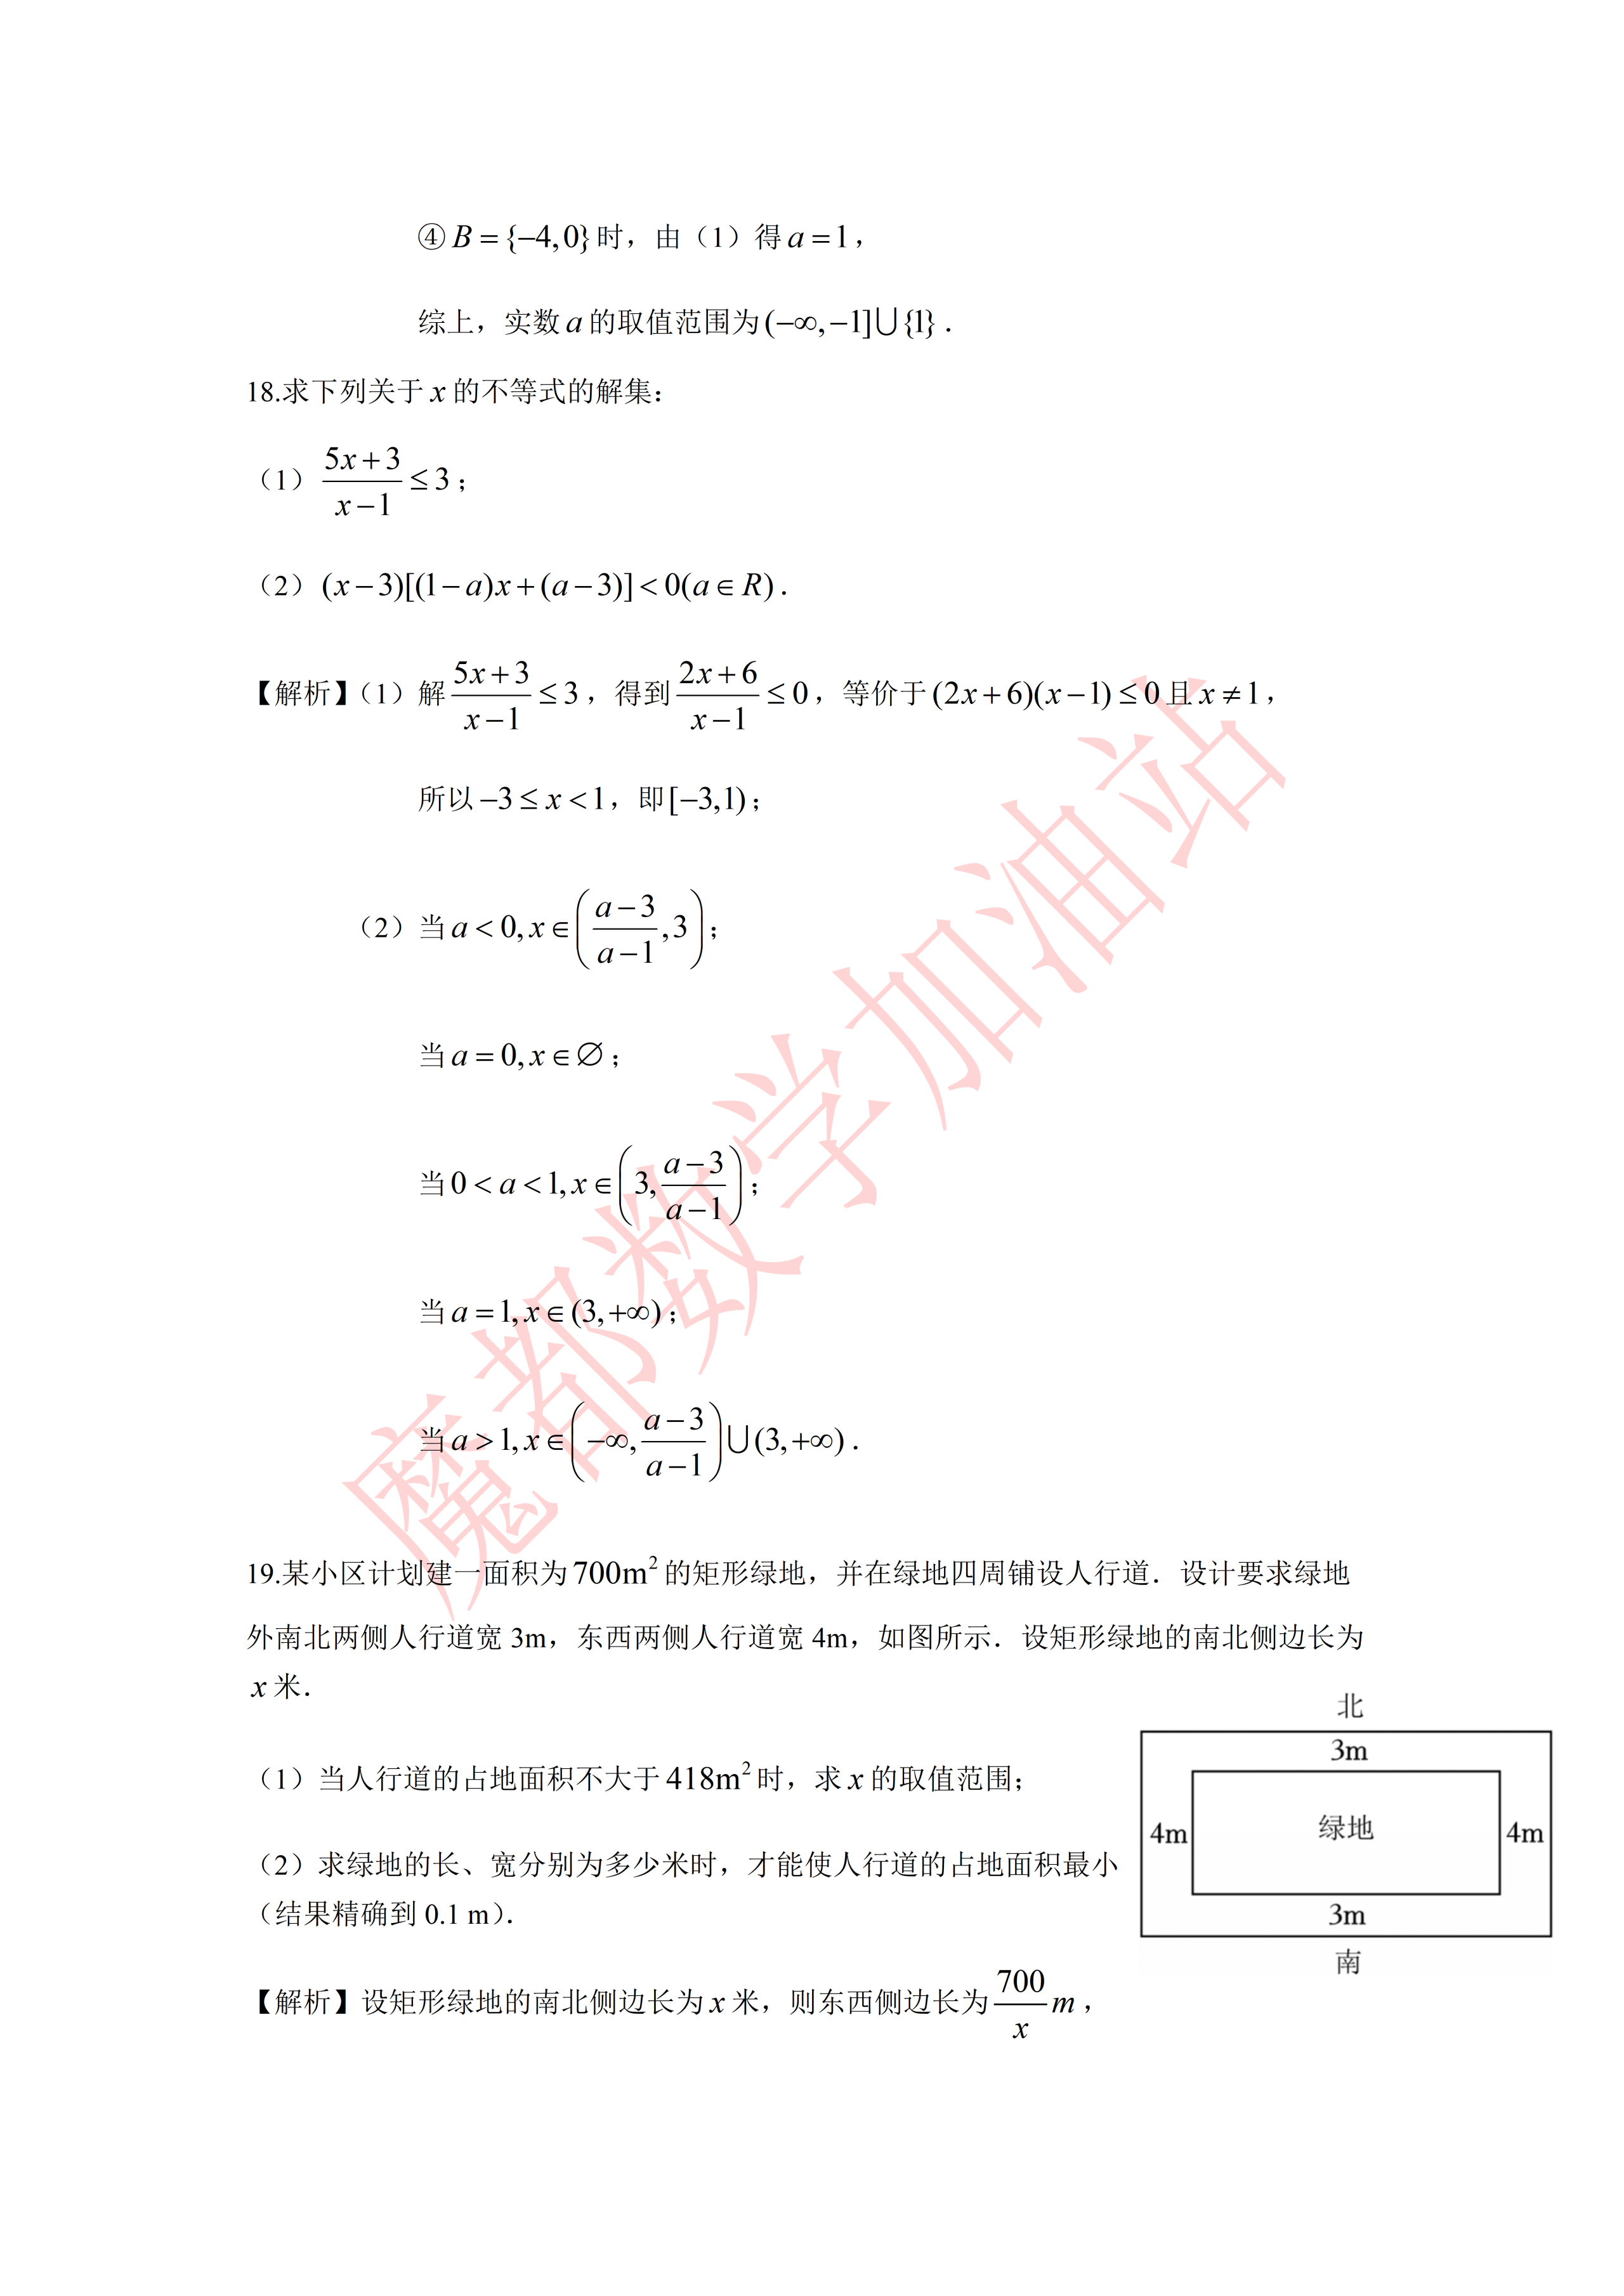
\includegraphics[width=.3\linewidth,trim=1791bp 484bp 107bp 2654bp,clip]{../原图/高一53_华师大二附中_10月月考/07.png}
\end{center}

\begin{enumerate}[label=(\arabic*)]
\item 当人行道的占地面积不大于 $418m^2$ 时，求 $x$ 的取值范围；
\item 求绿地的长、宽分别为多少米时，才能使人行道的占地面积最小（结果精确到 $0.1m$）.
\end{enumerate}

\ifanswer
\solbegin
\step{设矩形绿地的南北侧边长为 $x$ 米，则东西侧边长为 $\dfrac{700}{x}m$，}
\step{则人行道的占地面积为 $S=(x+8)\left(\dfrac{700}{x}+6\right)-700$，即 $S=6x+\dfrac{5600}{x}+48$.}
\stepm{(1)}{当人行道的占地面积不大于 $418m^2$ 时，$6x+\dfrac{5600}{x}+48\leqslant418$，}
\step{即 $6x^2-370x+5600\leqslant0$，解得 $\dfrac{80}{3}\leqslant x\leqslant35$，}
\step{故当人行道的占地面积不大于 $418m^2$ 时，$x\in\left[\dfrac{80}{3},35\right]$；}
\stepm{(2)}{$S=6x+\dfrac{5600}{x}+48\geqslant2\sqrt{6x\cdot\dfrac{5600}{x}}+48=80\sqrt{21}+48$，}
\step{当且仅当 $6x=\dfrac{5600}{x}$，即 $x=20\sqrt{\dfrac73}\approx30.6(m)$ 时，}
% 原卷如此，照录未改（80√21+48≈414.6，两处“414.4”疑笔误，见文件头“原卷笔误/存疑”第 6 条）
\step{$S$ 达到最小值 $80\sqrt{21}+48\approx414.4$，此时 $\dfrac{700}{x}\approx22.9(m)$，}
\step{所以当设计绿地的南北侧边长约为 $30.6m$，东西侧边长约为 $22.9m$ 时，}
\step{人行道的占地面积最小值为 $414.4(m^2)$.}
\solend
\fi

\ansspace[6]

\item 已知 $x\in\R$，符号 $[x]$ 表示不大于 $x$ 的最大整数，例如：$[2.3]=2$,$[2]=2$，$[-1.2]=-2$，令 $S(x)=[x]-[-x]$.

\begin{enumerate}[label=(\arabic*)]
\item 写出 $S(x)$ 为偶数（包括正、负偶数和 0）的充要条件，并证明；
\item 设方程 $|S(x)|=3$ 的解集为 $A$.

①集合 $B=\{x\mid x^2-ax-9\leqslant0,a\in\R\}$，若 $A\cap B=A$，求实数 $a$ 的取值范围；

②集合 $C=\{x\mid 2x^2-5kx+3k^2\geqslant0\}$，若 $A\cup C=\R$，求实数 $k$ 的取值范围.
\end{enumerate}

\ifanswer
\solbegin
\stepm{(1)}{$S(x)$ 为偶数的充要条件是 $x\in\Z$.}
\step{若 $x\in\Z$，则 $S(x)=[x]-[-x]=x-(-x)=2x$；}
\step{若 $x\notin\Z$，设 $[x]=n$，}
\step{则 $S(x)=[x]-[-x]=n-(-n-1)=2n+1=2[x]+1$；}
% 原卷如此，照录未改（“由①”按文意应为“由(1)”，见文件头“原卷笔误/存疑”第 3 条）
\stepm{(2)}{由①得 3 是奇数，$S(x)=\pm3$,$x\notin\Z$，}
\step{$S(x)=2[x]+1=\pm3$,$[x]=1$ 或 $-2$ 且 $x\notin\Z$，}
\step{所以 $A=(-2,-1)\cup(1,2)$；}
\stepm{①}{$A\cap B=A\Rightarrow A\subseteq B$，}
\step{设 $B=[x_1,x_2]$，其中 $x_1,x_2$ 是方程 $x^2-ax-9=0$ 的两实根，}
\step{设 $f(x)=x^2-ax-9$，}
\step{$[-2,2]\subseteq[x_1,x_2]\Leftrightarrow x_1\leqslant-2$,$x_2\geqslant2\Leftrightarrow\begin{cases}f(-2)\leqslant0\\ f(2)\leqslant0\end{cases}$}
\step{$\Leftrightarrow\begin{cases}(-2)^2-a\cdot(-2)-9\leqslant0, & a\leqslant\dfrac52\\ 2^2-2a-9\leqslant0, & a\geqslant-\dfrac52\end{cases}$，故 $a\in\left[-\dfrac52,\dfrac52\right]$；}
\step{注：若用求根公式 $\begin{cases}\dfrac{a+\sqrt{a^2+36}}{2}\geqslant2\Rightarrow a\geqslant-\dfrac52\\ \dfrac{a-\sqrt{a^2+36}}{2}\leqslant-2\Rightarrow a\leqslant\dfrac52\end{cases}$，结果正确，也得满分；}
\stepm{②}{$2x^2-5kx+3k^2=(x-k)(2x-3k)$.}
\step{$A\cup C=\R\Leftrightarrow\complement_\R A\subseteq C$.}
\step{记 $g(x)=2x^2-5kx+3k^2$，则 $\{x\mid g(x)<0\}\subseteq A$.}
\stepm{情况1：}{$k>0$ 时，$k<\dfrac32k$,$g(x)<0$ 的解集为 $\left(k,\dfrac32k\right)\subseteq(1,2)$，}
\step{故 $\begin{cases}k\geqslant1\\ \dfrac32k\leqslant2\end{cases}\Rightarrow1\leqslant k\leqslant\dfrac43$；}
\stepm{情况2：}{$k=0$ 时，$g(x)=2x^2\geqslant0$ 恒成立，$C=\R$,$A\cup C=\R$ 显然成立；}
\stepm{情况3：}{$k<0$ 时，$\dfrac32k<k$,$g(x)<0$ 的解集为 $\left(\dfrac32k,k\right)\subseteq(-2,-1)$，}
\step{故 $\begin{cases}\dfrac32k\geqslant-2\\ k\leqslant-1\end{cases}\Rightarrow-\dfrac43\leqslant k\leqslant-1$；}
\step{综上，$k\in\left[-\dfrac43,-1\right]\cup\{0\}\cup\left[1,\dfrac43\right]$.}
\solend
\fi

\ansspace[10]

\item 对于非空实数集 $M\subseteq(0,+\infty)$，若满足以下两个条件，则称 $M$ 为“极闭集”：

①$M$ 中至少含有 2 个元素，且 $1\notin M$；

②对于 $M$ 中任意两个不相等的元素 $x,y$，定义 $x*y=\dfrac{xy+1}{x+y}$，且 $x*y\in M$.

\begin{enumerate}[label=(\arabic*)]
\item 判断集合 $A=\left\{\dfrac12,2\right\}$ 与区间 $B=(1,+\infty)$ 是否为“极闭集”，并说明理由；
\item 若 $M$ 是“极闭集”，证明：集合 $M$ 中不可能所有元素都小于 1；
\item 证明：不存在任何有限的“极闭集”.
\end{enumerate}

\ifanswer
\solbegin
% 原卷如此，照录未改（首行集合按题干应为 {1/2,2}，见文件头“原卷笔误/存疑”第 7 条）
\stepm{(1)}{对于集合 $A=\left\{\dfrac12,1\right\}$，$\dfrac12*2=\dfrac45$，}
\step{因为 $\dfrac45\notin A$，不满足条件②，所以集合 $A$ 不是“极闭集”.}
\step{对于区间 $B$，满足条件①.}
\step{任取 $B$ 中两个不相等的元素 $x,y$，则 $x>1$,$y>1$.}
\step{$x*y-1=\dfrac{xy+1}{x+y}-1=\dfrac{(x-1)(y-1)}{x+y}>0$，所以 $x*y>1$，}
\step{这说明 $x*y\in B$ 恒成立，满足条件②，所以 $B$ 是“极闭集”.}
\stepm{(2)}{假设集合 $M$ 中所有元素都小于 1，}
\step{在 $M$ 中取 $0<x<y<1$,$x*y-1=\dfrac{xy+1}{x+y}-1=\dfrac{(x-1)(y-1)}{x+y}>0$，}
\step{所以 $x*y>1$，与“集合 $M$ 中所有元素都小于 1”矛盾，}
\step{假设不成立，集合 $M$ 中不可能所有元素都小于 1，得证.}
\stepm{(3)}{由②得，任何一个“极闭集”$M$ 中，必然至少存在一个大于 1 的元素，}
\stepm{情况1：}{若 $M$ 中至少存在两个大于 1 的元素，}
\step{设其中两个不相等的元素为 $x$ 和 $y_1$，且 $x>y_1>1$，}
\step{令 $y_{n+1}=x*y_n$,$n\geqslant1$,$y_{n+1}-1=x*y_n-1=\dfrac{(x-1)(y_n-1)}{xy_n+1}>0$，}
\step{如果 $y_n\geqslant1$，则显然 $y_{n+1}\geqslant1$，作差 $y_n-y_{n+1}=\dfrac{y_n^2-1}{x+y_n}>0$，}
\step{由此 $x>y_1>y_2>y_3>\cdots>1$，与有限集矛盾.}
\stepm{情况2：}{若 $M$ 中恰好只有一个元素大于 1，}
\step{设这个唯一大于 1 的元素为 $m$.}
\step{因为 $M$ 至少有两个元素，所以 $M$ 中必然至少存在一个元素 $a_1<1$，}
\step{令 $a_{n+1}=m*a_n$,$n\geqslant1$，}
\step{又 $a_{n+1}-1=m*a_n-1=\dfrac{(m-1)(a_n-1)}{m+a_n}<0$，故 $a_{n+1}<1$，}
\step{作差 $a_{n+1}-a_n=\dfrac{1-a_n^2}{m+a_n}>0$，由此 $a_1<a_2<a_3<\cdots<1$，与有限集矛盾.}
\step{因此，不存在任何有限的“极闭集”. 原命题得证.}
\solend
\fi

\ansspace*[10]

\end{enumerate}

\end{document}
"
% 紧凑版：xelatex "\def\iscompact{1}% 高一53_华师大二附中_10月月考.tex
%   —— 高一上数学“2026-2027 年华师大二附中高一上 10 月月考”（讲评版）
% 试卷版：xelatex 高一53_华师大二附中_10月月考.tex
% 答案版：xelatex "\def\isanswer{1}\input{高一53_华师大二附中_10月月考.tex}"
% 紧凑版：xelatex "\def\iscompact{1}\input{高一53_华师大二附中_10月月考.tex}"
%
% 原始材料：微信公众号“魔都数学加油站”文章，作者破晓，连载“27学年高一53”；
% 原文标题“27学年高一53——2026-2027年上海市华师大二附中高一上10月月考”；
% 原文链接：https://mp.weixin.qq.com/s/fpSnoF-gJEEWyxAoPC_bZA。
% 页面标注发布时间 2026-10-09 17:15（上海）。
% 正文为 11 张 PNG 页：第 01—06、08、10 页 4762×6735，第 07、09、11 页 2560×3620
% （**同一篇各页分辨率不同**），均按页序读取。11 页全为试卷正文页（卷首标题在第 1 页页顶，
% 卷末解答题第 21 题解析止于第 11 页），无封面页、目录页、二维码或宣传页。
% 粉色斜排“魔都数学加油站”为卷面水印，与公众号页脚一并未录入。
%
% 卷首标题：照卷面印作“2026--2027 年华师大二附中高一上 10 月月考”（公众号标题中的“上海市”
% 卷面标题行没有，本稿照卷面），年份区间按全稿惯例排 en dash。原卷只有一行标题、无副标题。
%
% 篇幅与题号：原卷自第 3 题起编号（第 1、2 题不在本卷内）。填空题 3—12（10 题）、
% 选择题 13—16（4 题）、解答题 17—21（5 题），共 19 题。本稿沿用原节与原题号，
% 只改排为全稿统一的大节样式（原卷小节标题为“一、填空题”“二、选择题”“三、解答题”）。
%
% 讲评版：原卷每题下直接印【答案】或【解析】。**第 13 题没有任何【答案】/【解析】段**，
% 答案“C”直接印在题干括号内（“一定不是(  C  )”），本稿按 高一37 第 13 题的成例把括号留空、
% 答案另提为 \ans{$C$}；其余 18 题都只印【解析】，按全稿口径这类题不另提 \ans{}——其中
% 选择题第 14、15、16 题的结论写在解析末句（“故选 B／D／C”），亦照录在解析内。
%
% 副标题：原卷未印副标题。本稿按“知识模块”口径标作“集合与常用逻辑用语、不等式”：
% 19 题中集合与常用逻辑用语 12 题（集合类 9 题——第 4、5、12、13、15、16、17、20、21 题；
% 逻辑类 3 题——第 3、9、14 题），不等式 7 题（含一元二次方程与绝对值方程：第 6、7、8、10、
% 11、18、19 题，其中第 11 题实为奇偶分析下的集合计数题，暂挂不等式），两类均超三分之一，
% 故并标。口径同 高一46、高一47、高一48、高一51、高一52。
%
% 与原卷的排版差异：
%   ① 原卷每题下直接印【解析】，本稿按全稿惯例将答案与解析置于答案版，试卷版保持干净；
%      第 13 题印在题干括号内的答案“C”同样移入 \ans{}，见上；
%   ② 原卷未印副标题，本稿按“知识模块”口径补出；
%   ③ 原卷填空横线约两个字宽，本稿按全稿惯例统一排 \blankline[4.4em]；
%      选择题的作答括号原卷排半角“(    )”，本稿按全稿惯例排 \mbox{（\quad）}；
%   ④ 原卷实数集排斜体/粗体 $R$、$\mathbf{R}$（第 4、6、7、18、20 题等处），本稿按全稿惯例
%      改用 $\R$；空集记号统一为 \varnothing；
%   ⑤ 原卷在数学式内多处用半角逗号（如 $x_1,x_2$、$|S|,|T|$、$a\neq0,c\neq0$），均照录未强改；
%      句末句点按全稿惯例排西文句点（原卷“故选 B．”一类全角句点亦从宽排作“.”）；
%   ⑥ 第 17—21 题的子问原卷各自另起一行，本稿按全稿惯例用 enumerate 的 (1)(2)(3)；
%      第 20 题 (2) 问下的①②两行是题干的一部分，照录为行首①②标号（不入 enumerate）；
%      解析中的子问标号一律用 \stepm{(1)}{…}，解析中的①②③④分情形用 \stepm{①}{…}；
%   ⑦ 第 12、20、21 题解析里的“情况1:”至“情况3:”标号原卷排**红色加粗**（全卷共 6 处），
%      全库无红色排字先例，本稿按全稿子题标号样式排 \stepm{情况1：}{…}（加粗着色、不改黑色基调），
%      冒号照原卷排全角；
%   ⑧ 第 19 题的示意图原卷排在题干右侧（与题干、(1) 问同高），本稿居中排在题干之后、
%      子问之前，并在 \item 前加 \needvspace 整块推走；图自原图第 07 页裁切（trim），不另存图片文件；
%   ⑨ 每道解答题原卷未留作答空白，本稿按全稿惯例加 \ansspace。
%
% 原卷笔误/存疑（均照录未改，正文对应处另有 % 注）：
%   1. 第 14 题解析末行“例如 $a=1$，$b=-1$，及必要性不成立”，“及”按文意应为“即”；
%   2. 第 15 题解析第 3 行 $\dfrac1{a+b\sqrt2}=\dfrac a{a^2-2b}+\left(-\dfrac b{a^2-2b}\right)\cdot\sqrt2$，
%      分母两处均作 $a^2-2b$，按通分应为 $a^2-2b^2$（结论 $C=X$ 不受影响）；
%   3. 第 20 题 (2) 问解析首行“由①得 3 是奇数”，按文意应为“由(1)得”（①是 (2) 问下自己
%      的子问标号，奇偶性结论出自 (1) 问）；
%   4. 第 11 题解析“只有奇数的有 $C_4^2+1=7$ 个”，按组合意义应为 $C_4^2+C_4^4=7$
%      （“$+1$”当指 4 个奇数全取的 1 种），数值无误；
%   5. 第 18 题 (2) 问解析“当 $a=0$,$x\in\varnothing$”，按文意应为“解集为 $\varnothing$”；
%   6. 第 19 题 (2) 问解析“$S$ 达到最小值 $80\sqrt{21}+48\approx414.4$”与末行
%      “人行道的占地面积最小值为 $414.4(m^2)$”，两处按 $80\sqrt{21}+48\approx414.6$，疑笔误；
%   7. 第 21 题 (1) 问解析首行“对于集合 $A=\left\{\frac12,1\right\}$”，按题干应为
%      $A=\left\{\frac12,2\right\}$（计算 $\frac12*2=\frac45$ 用的正是 $2$）；
%   8. 第 12 题解析“所以 $A=(-\infty,-4]\cup[2,+\infty)$”一行行末无标点，体例不一，照录。
%
% 插图：1 张，自原图裁切（无 \begin{tikzpicture} 重排）：
%   · 第 19 题绿地示意图（外矩形内套矩形“绿地”，上“北 3m”、下“南 3m”、左右各“4m”）
%     ——原图第 07 页，原卷排于题干右侧。
%     裁框：x 1797–2447、y 2660–3136（含“北”“南”标注，四周各留约 6px），
%     trim=1791bp 484bp 107bp 2654bp（左／下／右／上），页宽 2560、页高 3620。
%
\documentclass[a4paper,11pt]{article}
\usepackage{common}

\begin{document}

\examtitlest[3]{2026--2027 年华师大二附中高一上 10 月月考}{集合与常用逻辑用语、不等式}

\bigsec{一、填空题}

\begin{enumerate}
\setcounter{enumi}{2}

\item “$x=2$”是“$x^2-3x+2=0$”的\blankline[4.4em]条件.

（选择其中之一填空：充分非必要、必要非充分、充分、既非充分又非必要）

\ifanswer
\solbegin
\step{由 $x^2-3x+2=0$ 得 $x=1$ 或 $x=2$，}
\step{则“$x=2$”是“$x^2-3x+2=0$”的充分不必要条件.}
\solend
\fi

\item 已知 $R$ 是全集，集合 $A=\{y\mid y=-x^2+1,x\in\R\}$，集合 $B=\{x\mid x=3+|a|,a\in\R\}$，则 $\overline{A\cup B}=$\blankline[4.4em].

\ifanswer
\solbegin
\step{$A=\{y\mid y=-x^2+1,x\in\R\}=(-\infty,1]$，$B=\{x\mid x=3+|a|,a\in\R\}=[3,+\infty)$，}
\step{所以 $\overline{A\cup B}=(1,3)$.}
\solend
\fi

\item 已知 $a$ 为常数，集合 $A=\{x\mid x^2+x-6=0\}$，集合 $B=\{x\mid ax-2=0\}$，且 $B\subseteq A$，则 $a$ 的所有取值构成的集合为\blankline[4.4em].

\ifanswer
\solbegin
\step{集合 $A=\{-3,2\}$，因为 $B\subseteq A$，则 $B=\varnothing$，$\{-3\}$，$\{2\}$，$\{-3,2\}$，}
\step{当 $B=\varnothing$ 时，$a=0$，当 $B=\{-3\}$ 时，$a=-\dfrac23$，当 $B=\{2\}$ 时，$a=1$，}
\step{当 $B=\{-3,2\}$ 时，不成立，故 $a$ 的取值集合为 $\left\{0,-\dfrac23,1\right\}$.}
\solend
\fi

\item 设 $a\in\R$，若关于 $x$ 的不等式 $x^2-ax<0$ 的解集是区间 $(0,1)$ 的真子集，则 $a$ 的取值范围是\blankline[4.4em].

\ifanswer
\solbegin
\step{因为关于 $x$ 的不等式 $x^2-ax<0$ 的解集是区间 $(0,1)$ 的真子集，}
\step{当 $a=0$ 时，不等式的解集为 $\varnothing$，符合题意；}
\step{当 $a>0$ 时，不等式的解集为 $(0,a)$，则 $0<a<1$，}
\step{当 $a<0$ 时，不等式的解集为 $(a,0)$，不符合题意，}
\step{故 $a$ 的范围为 $[0,1)$.}
\solend
\fi

\item 设 $x\in\R$，则方程 $|2x+3|-|x-2|=|3x+1|$ 的解集为\blankline[4.4em].

\ifanswer
\solbegin
\step{当 $x\leqslant-\dfrac32$ 时，原式$\Leftrightarrow-2x-3+x-2=-3x-1\Leftrightarrow x=2$，不合题意；}
\step{当 $-\dfrac32<x\leqslant-\dfrac13$ 时，原式$\Leftrightarrow2x+3+x-2=-3x-1\Leftrightarrow x=-\dfrac13$；}
\step{当 $-\dfrac13<x\leqslant2$ 时，原式$\Leftrightarrow2x+3+x-2=3x+1\Leftrightarrow1=1$ 即恒成立；}
\step{当 $x>2$ 时，原式$\Leftrightarrow2x+3+2-x=3x+1\Leftrightarrow x=2$，不合题意；}
\step{故 $x\in\left[-\dfrac13,2\right]$.}
\solend
\fi

\item 已知关于 $x$ 的一元二次方程 $x^2+(4m+1)x+2m-1=0$．若方程的两根为 $x_1$、$x_2$，且满足 $\dfrac1{x_1}+\dfrac1{x_2}=-\dfrac12$，则实数 $m=$\blankline[4.4em].

\ifanswer
\solbegin
\step{由于判别式$\Delta=16m^2+5>0$恒成立，}
\step{不论 $m$ 为任何实数，方程总有两个不相等的实数根.}
\step{$\dfrac1{x_1}+\dfrac1{x_2}=-\dfrac12$，即 $\dfrac{x_1+x_2}{x_1x_2}=-\dfrac12$，由根与系数的关系得 $\dfrac{-4m-1}{2m-1}=-\dfrac12$，}
\step{解得 $m=-\dfrac12$.}
\solend
\fi

\item 已知 $\dfrac1{x-2}\geqslant1$ 是 $|x-a|<2$ 的充分非必要条件，则实数 $a$ 的取值范围是\blankline[4.4em].

\ifanswer
\solbegin
\step{由 $\dfrac1{x-2}\geqslant1$ 得 $\dfrac{3-x}{x-2}\geqslant0$，解得 $2<x\leqslant3$，由 $|x-a|<2$ 得 $a-2<x<a+2$，}
\step{因为 $\dfrac1{x-2}\geqslant1$ 是 $|x-a|<2$ 的充分非必要条件，}
\step{所以 $\{x\mid 2<x\leqslant3\}\subset\{x\mid a-2<x<a+2\}$，所以 $\begin{cases}a-2\leqslant2\\ a+2>3\end{cases}$，解得 $1<a\leqslant4$，}
\step{即实数 $a$ 的取值范围是 $(1,4]$.}
\solend
\fi

\item 设 $x,y\in(0,+\infty)$，且 $x+4y=1$，则 $\dfrac1x+\dfrac1y$ 的最小值为\blankline[4.4em].

\ifanswer
\solbegin
\step{因为 $\dfrac1x+\dfrac1y=(x+4y)\left(\dfrac1x+\dfrac1y\right)=5+\dfrac{4y}{x}+\dfrac{x}{y}\geqslant5+2\sqrt{\dfrac{4y}{x}\cdot\dfrac{x}{y}}=9$，}
\step{当且仅当 $\dfrac{4y}{x}=\dfrac{x}{y}$，即 $x=2y$，即 $x=\dfrac13$,$y=\dfrac16$ 时取等号，故最小值为 $9$.}
\solend
\fi

\item 设非空集合 $Q\subseteq M$，当 $Q$ 中所有元素和为偶数时（集合为单元素时和为元素本身），称 $Q$ 是 $M$ 的偶子集. 若集合 $M=\{1,2,3,4,5,6,7\}$，则其偶子集 $Q$ 的个数为\blankline[4.4em].

\ifanswer
\solbegin
\step{偶子集可以分为只有奇数、偶数及偶数个奇数和偶数的集合，}
\step{奇数有 4 个，偶数有 3 个，}
% 原卷如此，照录未改：按组合意义应为 C_4^2+C_4^4=7（“+1”当指 4 个奇数全取的 1 种），
% 见文件头“原卷笔误/存疑”第 4 条
\step{只有奇数的有 $C_4^2+1=7$ 个，只有偶数的有 $C_3^1+C_3^2+1=7$ 个，}
\step{偶数个奇数和偶数的：两奇一偶 $C_4^2\cdot C_3^1=18$ 个，两奇二偶 $C_4^2\cdot C_3^2=18$ 个，}
\step{两奇三偶 $C_4^2\cdot C_3^3=6$ 个，四奇一偶 $C_4^4\cdot C_3^1=3$ 个，四奇二偶 $C_4^4\cdot C_3^2=3$ 个，}
\step{四奇三偶 $C_4^4\cdot C_3^3=1$ 个，所以共有 $7+7+18+18+6+3+3+1=63$ 个.}
\solend
\fi

\item 已知集合 $A=\{x\mid x^2+2x-8\geqslant0\}$,$B=\{x\mid x^2-2ax+2a\leqslant0\}$，且 $A\cap B$ 中恰有 3 个整数元素，则实数 $a$ 的取值范围为\blankline[4.4em].

\ifanswer
\solbegin
% 原卷如此，照录未改：此行行末无标点，见文件头“原卷笔误/存疑”第 8 条
\step{由 $x^2+2x-8\geqslant0$，得 $x\geqslant2$ 或 $x\leqslant-4$，所以 $A=(-\infty,-4]\cup[2,+\infty)$}
\step{对集合 $B$：$x^2-2ax+2a\leqslant0$,$\Delta=4a^2-8a=4a(a-2)\geqslant0$，}
\step{得 $a\leqslant0$ 或 $a\geqslant2$.}
\step{设方程 $x^2-2ax+2a=0$ 的两根为 $r_1,r_2$，}
\step{则 $B=[r_1,r_2]$,$r_1=a-\sqrt{a^2-2a}$,$r_2=a+\sqrt{a^2-2a}$，}
\stepm{情况1：}{$a\leqslant0$，}
\step{$r_2=a+\sqrt{a^2-2a}<a+\sqrt{a^2-2a+1}=a+|a-1|=a+1-a=1<2$，}
\step{$B$ 只在 $A$ 的左侧部分有交集，要使 $A\cap B$ 恰有 3 个整数元素，}
\step{这 3 个整数为 $-6,-5,-4$，于是 $r_1\in(-7,-6]$，}
\step{令 $f(x)=x^2-2ax+2a$，则 $\begin{cases}f(-7)=49+14a+2a>0\\ f(-6)=36+12a+2a\leqslant0\end{cases}\Rightarrow a\in\left(-\dfrac{49}{16},-\dfrac{18}{7}\right]$；}
\stepm{情况2：}{$a\geqslant2$，}
\step{$r_2=a+\sqrt{a^2-2a}\geqslant2$，}
\step{$r_1=a-\sqrt{a^2-2a}>a-\sqrt{a^2-2a+1}=a-|a-1|=a-(a-1)=1>-4$，}
\step{所以 $A\cap B=[2,r_2]$.}
\step{同理 $\begin{cases}f(4)=16-8a+2a\leqslant0\\ f(5)=25-10a+2a>0\end{cases}\Rightarrow a\in\left[\dfrac{8}{3},\dfrac{25}{8}\right)$；}
\step{综上，$a\in\left(-\dfrac{49}{16},-\dfrac{18}{7}\right]\cup\left[\dfrac{8}{3},\dfrac{25}{8}\right)$.}
\solend
\fi

\end{enumerate}

\bigsec{二、选择题}

\begin{enumerate}
\setcounter{enumi}{12}

% 第 13 题原卷无【答案】/【解析】段，答案“C”直接印在题干括号内，
% 按高一37 第 13 题的成例括号留空、答案另提为 \ans{}（见文件头）
\item 集合 $A=\{a,b,c\}$ 中的三个元素分别表示某一个三角形的三边长度，那么这个三角形一定不是\mbox{（\quad）}

\keepwithprev
A. 锐角三角形\qquad B. 钝角三角形

C. 等腰三角形\qquad D. 直角三角形

\ifanswer
\ans{$C$}
\fi

\item 设 $a$、$b$ 为实数，则“$a<b<0$”是“$\dfrac1a>\dfrac1b$”的\mbox{（\quad）}条件.

\keepwithprev
A. 充要\qquad B. 充分不必要

C. 必要不充分\qquad D. 既不充分也不必要

\ifanswer
\solbegin
\step{若 $a<b<0$，则 $\dfrac1a>\dfrac1b$ 一定成立，即充分性成立；}
% 原卷如此，照录未改（“及”按文意应为“即”，见文件头“原卷笔误/存疑”第 1 条）
\step{若 $\dfrac1a>\dfrac1b$ 成立，$a<b<0$ 不一定成立，例如 $a=1$，$b=-1$，及必要性不成立.}
\step{故选 $B$.}
\solend
\fi

\item 设 $Q$ 表示有理数集，集合 $X=\{x\mid x=a+b\sqrt2,a,b\in Q,x\neq0\}$，在下列集合中：①$\{2x\mid x\in X\}$②$\left\{\dfrac{x}{\sqrt2}\mid x\in X\right\}$③$\left\{\dfrac1x\mid x\in X\right\}$④$\{x^2\mid x\in X\}$，与 $X$ 相同的集合有\mbox{（\quad）}

\keepwithprev
A. ①②③④\qquad B. ②③④\qquad C. ①②④\qquad D. ①②③

\ifanswer
\solbegin
\step{$A=\{2x\mid x\in X\}$，$2(a+b\sqrt2)=p+q\sqrt2$ 得 $p=2a$，$q=2b$，$a=\dfrac p2$，$b=\dfrac q2$，}
\step{也是一一对应，$A=X$}
% 原卷如此，照录未改：分母两处均作 a^2-2b，按通分应为 a^2-2b^2，
% 见文件头“原卷笔误/存疑”第 2 条
\step{集合 $B=\left\{\dfrac{x}{\sqrt2}\mid x\in X\right\}$，$\dfrac{a+b\sqrt2}{\sqrt2}=b+\dfrac a2\cdot\sqrt2$，也是一一对应，$B=X$}
\step{集合 $C=\left\{\dfrac1x\mid x\in X\right\}$，$\dfrac{1}{a+b\sqrt2}=\dfrac{a}{a^2-2b}+\left(-\dfrac{b}{a^2-2b}\right)\cdot\sqrt2$，一一对应，$C=X$}
\step{集合 $D=\{x^2\mid x\in X\}$，$(a+b\sqrt2)^2=a^2+2b^2+2ab\sqrt2$，这个不能一一对应了，}
\step{集合 $D$ 包含于 $X$ 中.}
\step{故 $X$ 相同的集合有①②③，故选 $D$.}
\solend
\fi

\item 集合 $S=\{x\mid(x+a)(x^2+bx+c)=0\}$,$T=\{x\mid(ax+1)(cx^2+bx+1)=0\}$，其中 $a,b,c$ 为实数，若 $|S|,|T|$ 分别表示集合 $S,T$ 的元素个数，则 $|S|-|T|$ 的所有可能取值集合为\mbox{（\quad）}

\keepwithprev
A. $\{0\}$\qquad B. $\{1\}$\qquad C. $\{0,1\}$\qquad D. $\{-1,0,1\}$

\ifanswer
\solbegin
\stepm{①}{$a\neq0,c\neq0$ 时.}
\step{$S$ 中 $x+a=0$ 的根 $x=-a$;$T$ 中 $ax+1=0$ 的根 $x=-\dfrac1a$.}
\step{$S$ 中的 $x^2+bx+c=0$ 若无实根，则 $T$ 中的 $cx^2+bx+1=0$ 也无实根；}
\step{又设 $S$ 的 $x^2+bx+c=0$ 的根为 $r(r\neq0)$，则 $T$ 的 $cx^2+bx+1=0$ 的根为 $\dfrac1r$.}
\step{（因为 $r^2+br+c=0\Rightarrow c\cdot\left(\dfrac1r\right)^2+b\cdot\dfrac1r+1=0$）}
\step{即 $a\neq0,c\neq0$ 时，}
\step{$S$ 与 $T$ 的实根存在一一对应关系 $x\leftrightarrow\dfrac1x$,$|S|=|T|,$$|S|-|T|=0$；}
\stepm{②}{$a=0,c\neq0$ 时.}
\step{$S$ 中多出一个根 $x=0$，而 $T$ 中无此根，$|S|=|T|+1$，即 $|S|-|T|=1$；}
\stepm{③}{$a\neq0,c=0$ 时.}
\step{则 $S$ 中仍有根 $x=0$，而 $T$ 中无 0 根，同样 $|S|-|T|=1$.}
\stepm{④}{$a=0,c=0$ 时.}
\step{同样 $S$ 含有根 0，而 $T$ 中不含 0，仍有 $|S|-|T|=1$.}
\step{综上，$|S|-|T|$ 所有可能取值为 0 和 1，故选 $C$.}
\solend
\fi

\end{enumerate}

\bigsec{三、解答题}

\begin{enumerate}
\setcounter{enumi}{16}

\item 已知集合 $A=\{x\mid x^2+4x=0\}$，$B=\{x\mid x^2+2(a+1)x+a^2-1=0\}$.

\begin{enumerate}[label=(\arabic*)]
\item 若 $A$ 是 $B$ 的子集，求实数 $a$ 的值；
\item 若 $B$ 是 $A$ 的子集，求实数 $a$ 的取值范围.
\end{enumerate}

\ifanswer
\solbegin
\stepm{(1)}{因为 $A=\{-4,0\}$，$B=\{x\mid x^2+2(a+1)x+a^2-1=0\}$，又 $A\subseteq B$，}
\step{所以 $A=B$，所以 $\begin{cases}-4+0=-2(a+1)\\ -4\times0=a^2-1\end{cases}$，所以 $a=1$；}
\stepm{(2)}{因为 $B$ 是 $A$ 的子集，所以 $B=\varnothing$ 或 $B=\{-4\}$ 或 $B=\{0\}$ 或 $B=\{-4,0\}$，}
\stepm{①}{$B=\varnothing$ 时，$\Delta=4(a+1)^2-4(a^2-1)<0$，所以 $a<-1$；}
\stepm{②}{$B=\{-4\}$ 时，$\begin{cases}-4+(-4)=-2(a+1)\\ -4\times(-4)=a^2-1\end{cases}$，无解；}
\stepm{③}{$B=\{0\}$ 时，$\begin{cases}0+0=-2(a+1)\\ 0\times0=a^2-1\end{cases}$，所以 $a=-1$；}
\stepm{④}{$B=\{-4,0\}$ 时，由（1）得 $a=1$，}
\step{综上，实数 $a$ 的取值范围为 $(-\infty,-1]\cup\{1\}$.}
\solend
\fi

\ansspace[6]

\item 求下列关于 $x$ 的不等式的解集：

\begin{enumerate}[label=(\arabic*)]
\item $\dfrac{5x+3}{x-1}\leqslant3$；
\item $(x-3)[(1-a)x+(a-3)]<0$ ($a\in\R$).
\end{enumerate}

\ifanswer
\solbegin
\stepm{(1)}{解 $\dfrac{5x+3}{x-1}\leqslant3$，得到 $\dfrac{2x+6}{x-1}\leqslant0$，等价于 $(2x+6)(x-1)\leqslant0$ 且 $x\neq1$，}
\step{所以 $-3\leqslant x<1$，即 $[-3,1)$；}
\stepm{(2)}{当 $a<0$,$x\in\left(\dfrac{a-3}{a-1},3\right)$；}
% 原卷如此，照录未改（“x∈∅”按文意应为“解集为 ∅”，见文件头“原卷笔误/存疑”第 5 条）
\step{当 $a=0$,$x\in\varnothing$；}
\step{当 $0<a<1$,$x\in\left(3,\dfrac{a-3}{a-1}\right)$；}
\step{当 $a=1$,$x\in(3,+\infty)$；}
\step{当 $a>1$,$x\in\left(-\infty,\dfrac{a-3}{a-1}\right)\cup(3,+\infty)$.}
\solend
\fi

\ansspace[6]

\needvspace{13\baselineskip}

\item 某小区计划建一面积为 $700m^2$ 的矩形绿地，并在绿地四周铺设人行道. 设计要求绿地外南北两侧人行道宽 $3m$，东西两侧人行道宽 $4m$，如图所示. 设矩形绿地的南北侧边长为 $x$ 米.

\begin{center}
% 原图第 7 页题干绿地示意图直接裁取（原卷排于题干右侧）。
% 裁框取图形外框 x 1797–2447、y 2660–3136（含“北”“南”标注，四周各留约 6px），
% trim=左 1791bp／下 484bp／右 107bp／上 2654bp（页宽 2560、页高 3620）。
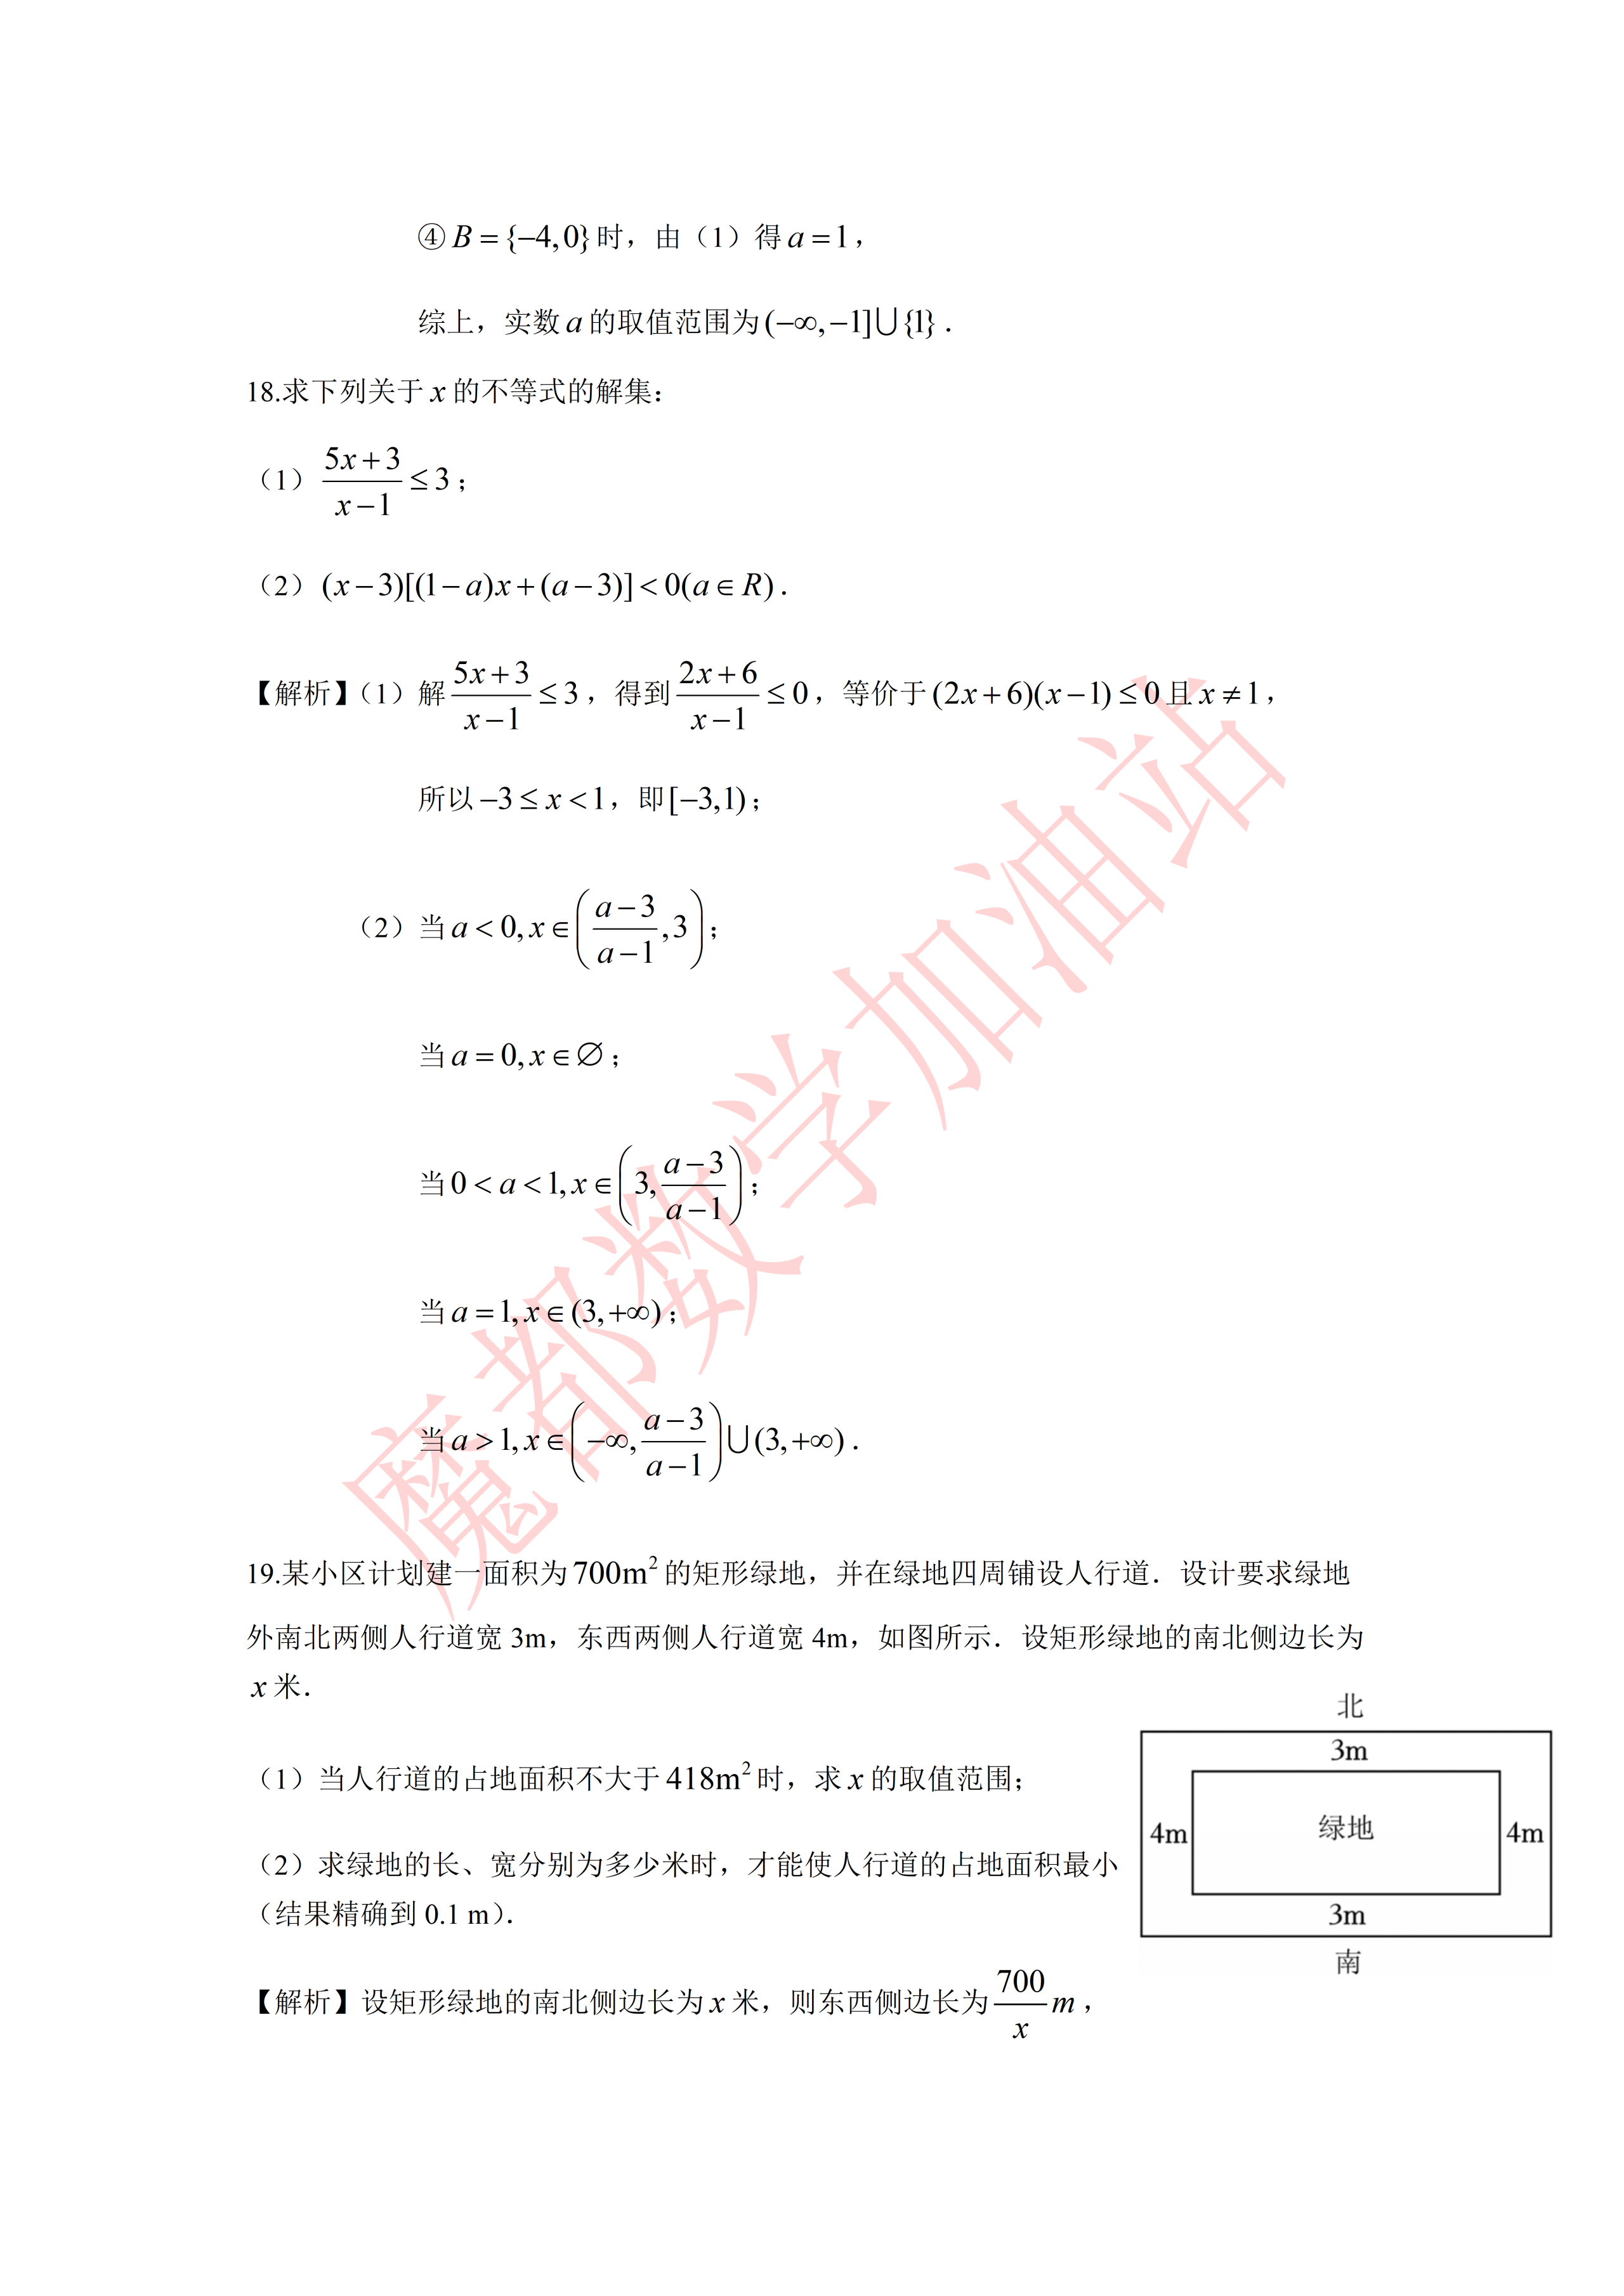
\includegraphics[width=.3\linewidth,trim=1791bp 484bp 107bp 2654bp,clip]{../原图/高一53_华师大二附中_10月月考/07.png}
\end{center}

\begin{enumerate}[label=(\arabic*)]
\item 当人行道的占地面积不大于 $418m^2$ 时，求 $x$ 的取值范围；
\item 求绿地的长、宽分别为多少米时，才能使人行道的占地面积最小（结果精确到 $0.1m$）.
\end{enumerate}

\ifanswer
\solbegin
\step{设矩形绿地的南北侧边长为 $x$ 米，则东西侧边长为 $\dfrac{700}{x}m$，}
\step{则人行道的占地面积为 $S=(x+8)\left(\dfrac{700}{x}+6\right)-700$，即 $S=6x+\dfrac{5600}{x}+48$.}
\stepm{(1)}{当人行道的占地面积不大于 $418m^2$ 时，$6x+\dfrac{5600}{x}+48\leqslant418$，}
\step{即 $6x^2-370x+5600\leqslant0$，解得 $\dfrac{80}{3}\leqslant x\leqslant35$，}
\step{故当人行道的占地面积不大于 $418m^2$ 时，$x\in\left[\dfrac{80}{3},35\right]$；}
\stepm{(2)}{$S=6x+\dfrac{5600}{x}+48\geqslant2\sqrt{6x\cdot\dfrac{5600}{x}}+48=80\sqrt{21}+48$，}
\step{当且仅当 $6x=\dfrac{5600}{x}$，即 $x=20\sqrt{\dfrac73}\approx30.6(m)$ 时，}
% 原卷如此，照录未改（80√21+48≈414.6，两处“414.4”疑笔误，见文件头“原卷笔误/存疑”第 6 条）
\step{$S$ 达到最小值 $80\sqrt{21}+48\approx414.4$，此时 $\dfrac{700}{x}\approx22.9(m)$，}
\step{所以当设计绿地的南北侧边长约为 $30.6m$，东西侧边长约为 $22.9m$ 时，}
\step{人行道的占地面积最小值为 $414.4(m^2)$.}
\solend
\fi

\ansspace[6]

\item 已知 $x\in\R$，符号 $[x]$ 表示不大于 $x$ 的最大整数，例如：$[2.3]=2$,$[2]=2$，$[-1.2]=-2$，令 $S(x)=[x]-[-x]$.

\begin{enumerate}[label=(\arabic*)]
\item 写出 $S(x)$ 为偶数（包括正、负偶数和 0）的充要条件，并证明；
\item 设方程 $|S(x)|=3$ 的解集为 $A$.

①集合 $B=\{x\mid x^2-ax-9\leqslant0,a\in\R\}$，若 $A\cap B=A$，求实数 $a$ 的取值范围；

②集合 $C=\{x\mid 2x^2-5kx+3k^2\geqslant0\}$，若 $A\cup C=\R$，求实数 $k$ 的取值范围.
\end{enumerate}

\ifanswer
\solbegin
\stepm{(1)}{$S(x)$ 为偶数的充要条件是 $x\in\Z$.}
\step{若 $x\in\Z$，则 $S(x)=[x]-[-x]=x-(-x)=2x$；}
\step{若 $x\notin\Z$，设 $[x]=n$，}
\step{则 $S(x)=[x]-[-x]=n-(-n-1)=2n+1=2[x]+1$；}
% 原卷如此，照录未改（“由①”按文意应为“由(1)”，见文件头“原卷笔误/存疑”第 3 条）
\stepm{(2)}{由①得 3 是奇数，$S(x)=\pm3$,$x\notin\Z$，}
\step{$S(x)=2[x]+1=\pm3$,$[x]=1$ 或 $-2$ 且 $x\notin\Z$，}
\step{所以 $A=(-2,-1)\cup(1,2)$；}
\stepm{①}{$A\cap B=A\Rightarrow A\subseteq B$，}
\step{设 $B=[x_1,x_2]$，其中 $x_1,x_2$ 是方程 $x^2-ax-9=0$ 的两实根，}
\step{设 $f(x)=x^2-ax-9$，}
\step{$[-2,2]\subseteq[x_1,x_2]\Leftrightarrow x_1\leqslant-2$,$x_2\geqslant2\Leftrightarrow\begin{cases}f(-2)\leqslant0\\ f(2)\leqslant0\end{cases}$}
\step{$\Leftrightarrow\begin{cases}(-2)^2-a\cdot(-2)-9\leqslant0, & a\leqslant\dfrac52\\ 2^2-2a-9\leqslant0, & a\geqslant-\dfrac52\end{cases}$，故 $a\in\left[-\dfrac52,\dfrac52\right]$；}
\step{注：若用求根公式 $\begin{cases}\dfrac{a+\sqrt{a^2+36}}{2}\geqslant2\Rightarrow a\geqslant-\dfrac52\\ \dfrac{a-\sqrt{a^2+36}}{2}\leqslant-2\Rightarrow a\leqslant\dfrac52\end{cases}$，结果正确，也得满分；}
\stepm{②}{$2x^2-5kx+3k^2=(x-k)(2x-3k)$.}
\step{$A\cup C=\R\Leftrightarrow\complement_\R A\subseteq C$.}
\step{记 $g(x)=2x^2-5kx+3k^2$，则 $\{x\mid g(x)<0\}\subseteq A$.}
\stepm{情况1：}{$k>0$ 时，$k<\dfrac32k$,$g(x)<0$ 的解集为 $\left(k,\dfrac32k\right)\subseteq(1,2)$，}
\step{故 $\begin{cases}k\geqslant1\\ \dfrac32k\leqslant2\end{cases}\Rightarrow1\leqslant k\leqslant\dfrac43$；}
\stepm{情况2：}{$k=0$ 时，$g(x)=2x^2\geqslant0$ 恒成立，$C=\R$,$A\cup C=\R$ 显然成立；}
\stepm{情况3：}{$k<0$ 时，$\dfrac32k<k$,$g(x)<0$ 的解集为 $\left(\dfrac32k,k\right)\subseteq(-2,-1)$，}
\step{故 $\begin{cases}\dfrac32k\geqslant-2\\ k\leqslant-1\end{cases}\Rightarrow-\dfrac43\leqslant k\leqslant-1$；}
\step{综上，$k\in\left[-\dfrac43,-1\right]\cup\{0\}\cup\left[1,\dfrac43\right]$.}
\solend
\fi

\ansspace[10]

\item 对于非空实数集 $M\subseteq(0,+\infty)$，若满足以下两个条件，则称 $M$ 为“极闭集”：

①$M$ 中至少含有 2 个元素，且 $1\notin M$；

②对于 $M$ 中任意两个不相等的元素 $x,y$，定义 $x*y=\dfrac{xy+1}{x+y}$，且 $x*y\in M$.

\begin{enumerate}[label=(\arabic*)]
\item 判断集合 $A=\left\{\dfrac12,2\right\}$ 与区间 $B=(1,+\infty)$ 是否为“极闭集”，并说明理由；
\item 若 $M$ 是“极闭集”，证明：集合 $M$ 中不可能所有元素都小于 1；
\item 证明：不存在任何有限的“极闭集”.
\end{enumerate}

\ifanswer
\solbegin
% 原卷如此，照录未改（首行集合按题干应为 {1/2,2}，见文件头“原卷笔误/存疑”第 7 条）
\stepm{(1)}{对于集合 $A=\left\{\dfrac12,1\right\}$，$\dfrac12*2=\dfrac45$，}
\step{因为 $\dfrac45\notin A$，不满足条件②，所以集合 $A$ 不是“极闭集”.}
\step{对于区间 $B$，满足条件①.}
\step{任取 $B$ 中两个不相等的元素 $x,y$，则 $x>1$,$y>1$.}
\step{$x*y-1=\dfrac{xy+1}{x+y}-1=\dfrac{(x-1)(y-1)}{x+y}>0$，所以 $x*y>1$，}
\step{这说明 $x*y\in B$ 恒成立，满足条件②，所以 $B$ 是“极闭集”.}
\stepm{(2)}{假设集合 $M$ 中所有元素都小于 1，}
\step{在 $M$ 中取 $0<x<y<1$,$x*y-1=\dfrac{xy+1}{x+y}-1=\dfrac{(x-1)(y-1)}{x+y}>0$，}
\step{所以 $x*y>1$，与“集合 $M$ 中所有元素都小于 1”矛盾，}
\step{假设不成立，集合 $M$ 中不可能所有元素都小于 1，得证.}
\stepm{(3)}{由②得，任何一个“极闭集”$M$ 中，必然至少存在一个大于 1 的元素，}
\stepm{情况1：}{若 $M$ 中至少存在两个大于 1 的元素，}
\step{设其中两个不相等的元素为 $x$ 和 $y_1$，且 $x>y_1>1$，}
\step{令 $y_{n+1}=x*y_n$,$n\geqslant1$,$y_{n+1}-1=x*y_n-1=\dfrac{(x-1)(y_n-1)}{xy_n+1}>0$，}
\step{如果 $y_n\geqslant1$，则显然 $y_{n+1}\geqslant1$，作差 $y_n-y_{n+1}=\dfrac{y_n^2-1}{x+y_n}>0$，}
\step{由此 $x>y_1>y_2>y_3>\cdots>1$，与有限集矛盾.}
\stepm{情况2：}{若 $M$ 中恰好只有一个元素大于 1，}
\step{设这个唯一大于 1 的元素为 $m$.}
\step{因为 $M$ 至少有两个元素，所以 $M$ 中必然至少存在一个元素 $a_1<1$，}
\step{令 $a_{n+1}=m*a_n$,$n\geqslant1$，}
\step{又 $a_{n+1}-1=m*a_n-1=\dfrac{(m-1)(a_n-1)}{m+a_n}<0$，故 $a_{n+1}<1$，}
\step{作差 $a_{n+1}-a_n=\dfrac{1-a_n^2}{m+a_n}>0$，由此 $a_1<a_2<a_3<\cdots<1$，与有限集矛盾.}
\step{因此，不存在任何有限的“极闭集”. 原命题得证.}
\solend
\fi

\ansspace*[10]

\end{enumerate}

\end{document}
"
%
% 原始材料：微信公众号“魔都数学加油站”文章，作者破晓，连载“27学年高一53”；
% 原文标题“27学年高一53——2026-2027年上海市华师大二附中高一上10月月考”；
% 原文链接：https://mp.weixin.qq.com/s/fpSnoF-gJEEWyxAoPC_bZA。
% 页面标注发布时间 2026-10-09 17:15（上海）。
% 正文为 11 张 PNG 页：第 01—06、08、10 页 4762×6735，第 07、09、11 页 2560×3620
% （**同一篇各页分辨率不同**），均按页序读取。11 页全为试卷正文页（卷首标题在第 1 页页顶，
% 卷末解答题第 21 题解析止于第 11 页），无封面页、目录页、二维码或宣传页。
% 粉色斜排“魔都数学加油站”为卷面水印，与公众号页脚一并未录入。
%
% 卷首标题：照卷面印作“2026--2027 年华师大二附中高一上 10 月月考”（公众号标题中的“上海市”
% 卷面标题行没有，本稿照卷面），年份区间按全稿惯例排 en dash。原卷只有一行标题、无副标题。
%
% 篇幅与题号：原卷自第 3 题起编号（第 1、2 题不在本卷内）。填空题 3—12（10 题）、
% 选择题 13—16（4 题）、解答题 17—21（5 题），共 19 题。本稿沿用原节与原题号，
% 只改排为全稿统一的大节样式（原卷小节标题为“一、填空题”“二、选择题”“三、解答题”）。
%
% 讲评版：原卷每题下直接印【答案】或【解析】。**第 13 题没有任何【答案】/【解析】段**，
% 答案“C”直接印在题干括号内（“一定不是(  C  )”），本稿按 高一37 第 13 题的成例把括号留空、
% 答案另提为 \ans{$C$}；其余 18 题都只印【解析】，按全稿口径这类题不另提 \ans{}——其中
% 选择题第 14、15、16 题的结论写在解析末句（“故选 B／D／C”），亦照录在解析内。
%
% 副标题：原卷未印副标题。本稿按“知识模块”口径标作“集合与常用逻辑用语、不等式”：
% 19 题中集合与常用逻辑用语 12 题（集合类 9 题——第 4、5、12、13、15、16、17、20、21 题；
% 逻辑类 3 题——第 3、9、14 题），不等式 7 题（含一元二次方程与绝对值方程：第 6、7、8、10、
% 11、18、19 题，其中第 11 题实为奇偶分析下的集合计数题，暂挂不等式），两类均超三分之一，
% 故并标。口径同 高一46、高一47、高一48、高一51、高一52。
%
% 与原卷的排版差异：
%   ① 原卷每题下直接印【解析】，本稿按全稿惯例将答案与解析置于答案版，试卷版保持干净；
%      第 13 题印在题干括号内的答案“C”同样移入 \ans{}，见上；
%   ② 原卷未印副标题，本稿按“知识模块”口径补出；
%   ③ 原卷填空横线约两个字宽，本稿按全稿惯例统一排 \blankline[4.4em]；
%      选择题的作答括号原卷排半角“(    )”，本稿按全稿惯例排 \mbox{（\quad）}；
%   ④ 原卷实数集排斜体/粗体 $R$、$\mathbf{R}$（第 4、6、7、18、20 题等处），本稿按全稿惯例
%      改用 $\R$；空集记号统一为 \varnothing；
%   ⑤ 原卷在数学式内多处用半角逗号（如 $x_1,x_2$、$|S|,|T|$、$a\neq0,c\neq0$），均照录未强改；
%      句末句点按全稿惯例排西文句点（原卷“故选 B．”一类全角句点亦从宽排作“.”）；
%   ⑥ 第 17—21 题的子问原卷各自另起一行，本稿按全稿惯例用 enumerate 的 (1)(2)(3)；
%      第 20 题 (2) 问下的①②两行是题干的一部分，照录为行首①②标号（不入 enumerate）；
%      解析中的子问标号一律用 \stepm{(1)}{…}，解析中的①②③④分情形用 \stepm{①}{…}；
%   ⑦ 第 12、20、21 题解析里的“情况1:”至“情况3:”标号原卷排**红色加粗**（全卷共 6 处），
%      全库无红色排字先例，本稿按全稿子题标号样式排 \stepm{情况1：}{…}（加粗着色、不改黑色基调），
%      冒号照原卷排全角；
%   ⑧ 第 19 题的示意图原卷排在题干右侧（与题干、(1) 问同高），本稿居中排在题干之后、
%      子问之前，并在 \item 前加 \needvspace 整块推走；图自原图第 07 页裁切（trim），不另存图片文件；
%   ⑨ 每道解答题原卷未留作答空白，本稿按全稿惯例加 \ansspace。
%
% 原卷笔误/存疑（均照录未改，正文对应处另有 % 注）：
%   1. 第 14 题解析末行“例如 $a=1$，$b=-1$，及必要性不成立”，“及”按文意应为“即”；
%   2. 第 15 题解析第 3 行 $\dfrac1{a+b\sqrt2}=\dfrac a{a^2-2b}+\left(-\dfrac b{a^2-2b}\right)\cdot\sqrt2$，
%      分母两处均作 $a^2-2b$，按通分应为 $a^2-2b^2$（结论 $C=X$ 不受影响）；
%   3. 第 20 题 (2) 问解析首行“由①得 3 是奇数”，按文意应为“由(1)得”（①是 (2) 问下自己
%      的子问标号，奇偶性结论出自 (1) 问）；
%   4. 第 11 题解析“只有奇数的有 $C_4^2+1=7$ 个”，按组合意义应为 $C_4^2+C_4^4=7$
%      （“$+1$”当指 4 个奇数全取的 1 种），数值无误；
%   5. 第 18 题 (2) 问解析“当 $a=0$,$x\in\varnothing$”，按文意应为“解集为 $\varnothing$”；
%   6. 第 19 题 (2) 问解析“$S$ 达到最小值 $80\sqrt{21}+48\approx414.4$”与末行
%      “人行道的占地面积最小值为 $414.4(m^2)$”，两处按 $80\sqrt{21}+48\approx414.6$，疑笔误；
%   7. 第 21 题 (1) 问解析首行“对于集合 $A=\left\{\frac12,1\right\}$”，按题干应为
%      $A=\left\{\frac12,2\right\}$（计算 $\frac12*2=\frac45$ 用的正是 $2$）；
%   8. 第 12 题解析“所以 $A=(-\infty,-4]\cup[2,+\infty)$”一行行末无标点，体例不一，照录。
%
% 插图：1 张，自原图裁切（无 \begin{tikzpicture} 重排）：
%   · 第 19 题绿地示意图（外矩形内套矩形“绿地”，上“北 3m”、下“南 3m”、左右各“4m”）
%     ——原图第 07 页，原卷排于题干右侧。
%     裁框：x 1797–2447、y 2660–3136（含“北”“南”标注，四周各留约 6px），
%     trim=1791bp 484bp 107bp 2654bp（左／下／右／上），页宽 2560、页高 3620。
%
\documentclass[a4paper,11pt]{article}
\usepackage{common}

\begin{document}

\examtitlest[3]{2026--2027 年华师大二附中高一上 10 月月考}{集合与常用逻辑用语、不等式}

\bigsec{一、填空题}

\begin{enumerate}
\setcounter{enumi}{2}

\item “$x=2$”是“$x^2-3x+2=0$”的\blankline[4.4em]条件.

（选择其中之一填空：充分非必要、必要非充分、充分、既非充分又非必要）

\ifanswer
\solbegin
\step{由 $x^2-3x+2=0$ 得 $x=1$ 或 $x=2$，}
\step{则“$x=2$”是“$x^2-3x+2=0$”的充分不必要条件.}
\solend
\fi

\item 已知 $R$ 是全集，集合 $A=\{y\mid y=-x^2+1,x\in\R\}$，集合 $B=\{x\mid x=3+|a|,a\in\R\}$，则 $\overline{A\cup B}=$\blankline[4.4em].

\ifanswer
\solbegin
\step{$A=\{y\mid y=-x^2+1,x\in\R\}=(-\infty,1]$，$B=\{x\mid x=3+|a|,a\in\R\}=[3,+\infty)$，}
\step{所以 $\overline{A\cup B}=(1,3)$.}
\solend
\fi

\item 已知 $a$ 为常数，集合 $A=\{x\mid x^2+x-6=0\}$，集合 $B=\{x\mid ax-2=0\}$，且 $B\subseteq A$，则 $a$ 的所有取值构成的集合为\blankline[4.4em].

\ifanswer
\solbegin
\step{集合 $A=\{-3,2\}$，因为 $B\subseteq A$，则 $B=\varnothing$，$\{-3\}$，$\{2\}$，$\{-3,2\}$，}
\step{当 $B=\varnothing$ 时，$a=0$，当 $B=\{-3\}$ 时，$a=-\dfrac23$，当 $B=\{2\}$ 时，$a=1$，}
\step{当 $B=\{-3,2\}$ 时，不成立，故 $a$ 的取值集合为 $\left\{0,-\dfrac23,1\right\}$.}
\solend
\fi

\item 设 $a\in\R$，若关于 $x$ 的不等式 $x^2-ax<0$ 的解集是区间 $(0,1)$ 的真子集，则 $a$ 的取值范围是\blankline[4.4em].

\ifanswer
\solbegin
\step{因为关于 $x$ 的不等式 $x^2-ax<0$ 的解集是区间 $(0,1)$ 的真子集，}
\step{当 $a=0$ 时，不等式的解集为 $\varnothing$，符合题意；}
\step{当 $a>0$ 时，不等式的解集为 $(0,a)$，则 $0<a<1$，}
\step{当 $a<0$ 时，不等式的解集为 $(a,0)$，不符合题意，}
\step{故 $a$ 的范围为 $[0,1)$.}
\solend
\fi

\item 设 $x\in\R$，则方程 $|2x+3|-|x-2|=|3x+1|$ 的解集为\blankline[4.4em].

\ifanswer
\solbegin
\step{当 $x\leqslant-\dfrac32$ 时，原式$\Leftrightarrow-2x-3+x-2=-3x-1\Leftrightarrow x=2$，不合题意；}
\step{当 $-\dfrac32<x\leqslant-\dfrac13$ 时，原式$\Leftrightarrow2x+3+x-2=-3x-1\Leftrightarrow x=-\dfrac13$；}
\step{当 $-\dfrac13<x\leqslant2$ 时，原式$\Leftrightarrow2x+3+x-2=3x+1\Leftrightarrow1=1$ 即恒成立；}
\step{当 $x>2$ 时，原式$\Leftrightarrow2x+3+2-x=3x+1\Leftrightarrow x=2$，不合题意；}
\step{故 $x\in\left[-\dfrac13,2\right]$.}
\solend
\fi

\item 已知关于 $x$ 的一元二次方程 $x^2+(4m+1)x+2m-1=0$．若方程的两根为 $x_1$、$x_2$，且满足 $\dfrac1{x_1}+\dfrac1{x_2}=-\dfrac12$，则实数 $m=$\blankline[4.4em].

\ifanswer
\solbegin
\step{由于判别式$\Delta=16m^2+5>0$恒成立，}
\step{不论 $m$ 为任何实数，方程总有两个不相等的实数根.}
\step{$\dfrac1{x_1}+\dfrac1{x_2}=-\dfrac12$，即 $\dfrac{x_1+x_2}{x_1x_2}=-\dfrac12$，由根与系数的关系得 $\dfrac{-4m-1}{2m-1}=-\dfrac12$，}
\step{解得 $m=-\dfrac12$.}
\solend
\fi

\item 已知 $\dfrac1{x-2}\geqslant1$ 是 $|x-a|<2$ 的充分非必要条件，则实数 $a$ 的取值范围是\blankline[4.4em].

\ifanswer
\solbegin
\step{由 $\dfrac1{x-2}\geqslant1$ 得 $\dfrac{3-x}{x-2}\geqslant0$，解得 $2<x\leqslant3$，由 $|x-a|<2$ 得 $a-2<x<a+2$，}
\step{因为 $\dfrac1{x-2}\geqslant1$ 是 $|x-a|<2$ 的充分非必要条件，}
\step{所以 $\{x\mid 2<x\leqslant3\}\subset\{x\mid a-2<x<a+2\}$，所以 $\begin{cases}a-2\leqslant2\\ a+2>3\end{cases}$，解得 $1<a\leqslant4$，}
\step{即实数 $a$ 的取值范围是 $(1,4]$.}
\solend
\fi

\item 设 $x,y\in(0,+\infty)$，且 $x+4y=1$，则 $\dfrac1x+\dfrac1y$ 的最小值为\blankline[4.4em].

\ifanswer
\solbegin
\step{因为 $\dfrac1x+\dfrac1y=(x+4y)\left(\dfrac1x+\dfrac1y\right)=5+\dfrac{4y}{x}+\dfrac{x}{y}\geqslant5+2\sqrt{\dfrac{4y}{x}\cdot\dfrac{x}{y}}=9$，}
\step{当且仅当 $\dfrac{4y}{x}=\dfrac{x}{y}$，即 $x=2y$，即 $x=\dfrac13$,$y=\dfrac16$ 时取等号，故最小值为 $9$.}
\solend
\fi

\item 设非空集合 $Q\subseteq M$，当 $Q$ 中所有元素和为偶数时（集合为单元素时和为元素本身），称 $Q$ 是 $M$ 的偶子集. 若集合 $M=\{1,2,3,4,5,6,7\}$，则其偶子集 $Q$ 的个数为\blankline[4.4em].

\ifanswer
\solbegin
\step{偶子集可以分为只有奇数、偶数及偶数个奇数和偶数的集合，}
\step{奇数有 4 个，偶数有 3 个，}
% 原卷如此，照录未改：按组合意义应为 C_4^2+C_4^4=7（“+1”当指 4 个奇数全取的 1 种），
% 见文件头“原卷笔误/存疑”第 4 条
\step{只有奇数的有 $C_4^2+1=7$ 个，只有偶数的有 $C_3^1+C_3^2+1=7$ 个，}
\step{偶数个奇数和偶数的：两奇一偶 $C_4^2\cdot C_3^1=18$ 个，两奇二偶 $C_4^2\cdot C_3^2=18$ 个，}
\step{两奇三偶 $C_4^2\cdot C_3^3=6$ 个，四奇一偶 $C_4^4\cdot C_3^1=3$ 个，四奇二偶 $C_4^4\cdot C_3^2=3$ 个，}
\step{四奇三偶 $C_4^4\cdot C_3^3=1$ 个，所以共有 $7+7+18+18+6+3+3+1=63$ 个.}
\solend
\fi

\item 已知集合 $A=\{x\mid x^2+2x-8\geqslant0\}$,$B=\{x\mid x^2-2ax+2a\leqslant0\}$，且 $A\cap B$ 中恰有 3 个整数元素，则实数 $a$ 的取值范围为\blankline[4.4em].

\ifanswer
\solbegin
% 原卷如此，照录未改：此行行末无标点，见文件头“原卷笔误/存疑”第 8 条
\step{由 $x^2+2x-8\geqslant0$，得 $x\geqslant2$ 或 $x\leqslant-4$，所以 $A=(-\infty,-4]\cup[2,+\infty)$}
\step{对集合 $B$：$x^2-2ax+2a\leqslant0$,$\Delta=4a^2-8a=4a(a-2)\geqslant0$，}
\step{得 $a\leqslant0$ 或 $a\geqslant2$.}
\step{设方程 $x^2-2ax+2a=0$ 的两根为 $r_1,r_2$，}
\step{则 $B=[r_1,r_2]$,$r_1=a-\sqrt{a^2-2a}$,$r_2=a+\sqrt{a^2-2a}$，}
\stepm{情况1：}{$a\leqslant0$，}
\step{$r_2=a+\sqrt{a^2-2a}<a+\sqrt{a^2-2a+1}=a+|a-1|=a+1-a=1<2$，}
\step{$B$ 只在 $A$ 的左侧部分有交集，要使 $A\cap B$ 恰有 3 个整数元素，}
\step{这 3 个整数为 $-6,-5,-4$，于是 $r_1\in(-7,-6]$，}
\step{令 $f(x)=x^2-2ax+2a$，则 $\begin{cases}f(-7)=49+14a+2a>0\\ f(-6)=36+12a+2a\leqslant0\end{cases}\Rightarrow a\in\left(-\dfrac{49}{16},-\dfrac{18}{7}\right]$；}
\stepm{情况2：}{$a\geqslant2$，}
\step{$r_2=a+\sqrt{a^2-2a}\geqslant2$，}
\step{$r_1=a-\sqrt{a^2-2a}>a-\sqrt{a^2-2a+1}=a-|a-1|=a-(a-1)=1>-4$，}
\step{所以 $A\cap B=[2,r_2]$.}
\step{同理 $\begin{cases}f(4)=16-8a+2a\leqslant0\\ f(5)=25-10a+2a>0\end{cases}\Rightarrow a\in\left[\dfrac{8}{3},\dfrac{25}{8}\right)$；}
\step{综上，$a\in\left(-\dfrac{49}{16},-\dfrac{18}{7}\right]\cup\left[\dfrac{8}{3},\dfrac{25}{8}\right)$.}
\solend
\fi

\end{enumerate}

\bigsec{二、选择题}

\begin{enumerate}
\setcounter{enumi}{12}

% 第 13 题原卷无【答案】/【解析】段，答案“C”直接印在题干括号内，
% 按高一37 第 13 题的成例括号留空、答案另提为 \ans{}（见文件头）
\item 集合 $A=\{a,b,c\}$ 中的三个元素分别表示某一个三角形的三边长度，那么这个三角形一定不是\mbox{（\quad）}

\keepwithprev
A. 锐角三角形\qquad B. 钝角三角形

C. 等腰三角形\qquad D. 直角三角形

\ifanswer
\ans{$C$}
\fi

\item 设 $a$、$b$ 为实数，则“$a<b<0$”是“$\dfrac1a>\dfrac1b$”的\mbox{（\quad）}条件.

\keepwithprev
A. 充要\qquad B. 充分不必要

C. 必要不充分\qquad D. 既不充分也不必要

\ifanswer
\solbegin
\step{若 $a<b<0$，则 $\dfrac1a>\dfrac1b$ 一定成立，即充分性成立；}
% 原卷如此，照录未改（“及”按文意应为“即”，见文件头“原卷笔误/存疑”第 1 条）
\step{若 $\dfrac1a>\dfrac1b$ 成立，$a<b<0$ 不一定成立，例如 $a=1$，$b=-1$，及必要性不成立.}
\step{故选 $B$.}
\solend
\fi

\item 设 $Q$ 表示有理数集，集合 $X=\{x\mid x=a+b\sqrt2,a,b\in Q,x\neq0\}$，在下列集合中：①$\{2x\mid x\in X\}$②$\left\{\dfrac{x}{\sqrt2}\mid x\in X\right\}$③$\left\{\dfrac1x\mid x\in X\right\}$④$\{x^2\mid x\in X\}$，与 $X$ 相同的集合有\mbox{（\quad）}

\keepwithprev
A. ①②③④\qquad B. ②③④\qquad C. ①②④\qquad D. ①②③

\ifanswer
\solbegin
\step{$A=\{2x\mid x\in X\}$，$2(a+b\sqrt2)=p+q\sqrt2$ 得 $p=2a$，$q=2b$，$a=\dfrac p2$，$b=\dfrac q2$，}
\step{也是一一对应，$A=X$}
% 原卷如此，照录未改：分母两处均作 a^2-2b，按通分应为 a^2-2b^2，
% 见文件头“原卷笔误/存疑”第 2 条
\step{集合 $B=\left\{\dfrac{x}{\sqrt2}\mid x\in X\right\}$，$\dfrac{a+b\sqrt2}{\sqrt2}=b+\dfrac a2\cdot\sqrt2$，也是一一对应，$B=X$}
\step{集合 $C=\left\{\dfrac1x\mid x\in X\right\}$，$\dfrac{1}{a+b\sqrt2}=\dfrac{a}{a^2-2b}+\left(-\dfrac{b}{a^2-2b}\right)\cdot\sqrt2$，一一对应，$C=X$}
\step{集合 $D=\{x^2\mid x\in X\}$，$(a+b\sqrt2)^2=a^2+2b^2+2ab\sqrt2$，这个不能一一对应了，}
\step{集合 $D$ 包含于 $X$ 中.}
\step{故 $X$ 相同的集合有①②③，故选 $D$.}
\solend
\fi

\item 集合 $S=\{x\mid(x+a)(x^2+bx+c)=0\}$,$T=\{x\mid(ax+1)(cx^2+bx+1)=0\}$，其中 $a,b,c$ 为实数，若 $|S|,|T|$ 分别表示集合 $S,T$ 的元素个数，则 $|S|-|T|$ 的所有可能取值集合为\mbox{（\quad）}

\keepwithprev
A. $\{0\}$\qquad B. $\{1\}$\qquad C. $\{0,1\}$\qquad D. $\{-1,0,1\}$

\ifanswer
\solbegin
\stepm{①}{$a\neq0,c\neq0$ 时.}
\step{$S$ 中 $x+a=0$ 的根 $x=-a$;$T$ 中 $ax+1=0$ 的根 $x=-\dfrac1a$.}
\step{$S$ 中的 $x^2+bx+c=0$ 若无实根，则 $T$ 中的 $cx^2+bx+1=0$ 也无实根；}
\step{又设 $S$ 的 $x^2+bx+c=0$ 的根为 $r(r\neq0)$，则 $T$ 的 $cx^2+bx+1=0$ 的根为 $\dfrac1r$.}
\step{（因为 $r^2+br+c=0\Rightarrow c\cdot\left(\dfrac1r\right)^2+b\cdot\dfrac1r+1=0$）}
\step{即 $a\neq0,c\neq0$ 时，}
\step{$S$ 与 $T$ 的实根存在一一对应关系 $x\leftrightarrow\dfrac1x$,$|S|=|T|,$$|S|-|T|=0$；}
\stepm{②}{$a=0,c\neq0$ 时.}
\step{$S$ 中多出一个根 $x=0$，而 $T$ 中无此根，$|S|=|T|+1$，即 $|S|-|T|=1$；}
\stepm{③}{$a\neq0,c=0$ 时.}
\step{则 $S$ 中仍有根 $x=0$，而 $T$ 中无 0 根，同样 $|S|-|T|=1$.}
\stepm{④}{$a=0,c=0$ 时.}
\step{同样 $S$ 含有根 0，而 $T$ 中不含 0，仍有 $|S|-|T|=1$.}
\step{综上，$|S|-|T|$ 所有可能取值为 0 和 1，故选 $C$.}
\solend
\fi

\end{enumerate}

\bigsec{三、解答题}

\begin{enumerate}
\setcounter{enumi}{16}

\item 已知集合 $A=\{x\mid x^2+4x=0\}$，$B=\{x\mid x^2+2(a+1)x+a^2-1=0\}$.

\begin{enumerate}[label=(\arabic*)]
\item 若 $A$ 是 $B$ 的子集，求实数 $a$ 的值；
\item 若 $B$ 是 $A$ 的子集，求实数 $a$ 的取值范围.
\end{enumerate}

\ifanswer
\solbegin
\stepm{(1)}{因为 $A=\{-4,0\}$，$B=\{x\mid x^2+2(a+1)x+a^2-1=0\}$，又 $A\subseteq B$，}
\step{所以 $A=B$，所以 $\begin{cases}-4+0=-2(a+1)\\ -4\times0=a^2-1\end{cases}$，所以 $a=1$；}
\stepm{(2)}{因为 $B$ 是 $A$ 的子集，所以 $B=\varnothing$ 或 $B=\{-4\}$ 或 $B=\{0\}$ 或 $B=\{-4,0\}$，}
\stepm{①}{$B=\varnothing$ 时，$\Delta=4(a+1)^2-4(a^2-1)<0$，所以 $a<-1$；}
\stepm{②}{$B=\{-4\}$ 时，$\begin{cases}-4+(-4)=-2(a+1)\\ -4\times(-4)=a^2-1\end{cases}$，无解；}
\stepm{③}{$B=\{0\}$ 时，$\begin{cases}0+0=-2(a+1)\\ 0\times0=a^2-1\end{cases}$，所以 $a=-1$；}
\stepm{④}{$B=\{-4,0\}$ 时，由（1）得 $a=1$，}
\step{综上，实数 $a$ 的取值范围为 $(-\infty,-1]\cup\{1\}$.}
\solend
\fi

\ansspace[6]

\item 求下列关于 $x$ 的不等式的解集：

\begin{enumerate}[label=(\arabic*)]
\item $\dfrac{5x+3}{x-1}\leqslant3$；
\item $(x-3)[(1-a)x+(a-3)]<0$ ($a\in\R$).
\end{enumerate}

\ifanswer
\solbegin
\stepm{(1)}{解 $\dfrac{5x+3}{x-1}\leqslant3$，得到 $\dfrac{2x+6}{x-1}\leqslant0$，等价于 $(2x+6)(x-1)\leqslant0$ 且 $x\neq1$，}
\step{所以 $-3\leqslant x<1$，即 $[-3,1)$；}
\stepm{(2)}{当 $a<0$,$x\in\left(\dfrac{a-3}{a-1},3\right)$；}
% 原卷如此，照录未改（“x∈∅”按文意应为“解集为 ∅”，见文件头“原卷笔误/存疑”第 5 条）
\step{当 $a=0$,$x\in\varnothing$；}
\step{当 $0<a<1$,$x\in\left(3,\dfrac{a-3}{a-1}\right)$；}
\step{当 $a=1$,$x\in(3,+\infty)$；}
\step{当 $a>1$,$x\in\left(-\infty,\dfrac{a-3}{a-1}\right)\cup(3,+\infty)$.}
\solend
\fi

\ansspace[6]

\needvspace{13\baselineskip}

\item 某小区计划建一面积为 $700m^2$ 的矩形绿地，并在绿地四周铺设人行道. 设计要求绿地外南北两侧人行道宽 $3m$，东西两侧人行道宽 $4m$，如图所示. 设矩形绿地的南北侧边长为 $x$ 米.

\begin{center}
% 原图第 7 页题干绿地示意图直接裁取（原卷排于题干右侧）。
% 裁框取图形外框 x 1797–2447、y 2660–3136（含“北”“南”标注，四周各留约 6px），
% trim=左 1791bp／下 484bp／右 107bp／上 2654bp（页宽 2560、页高 3620）。
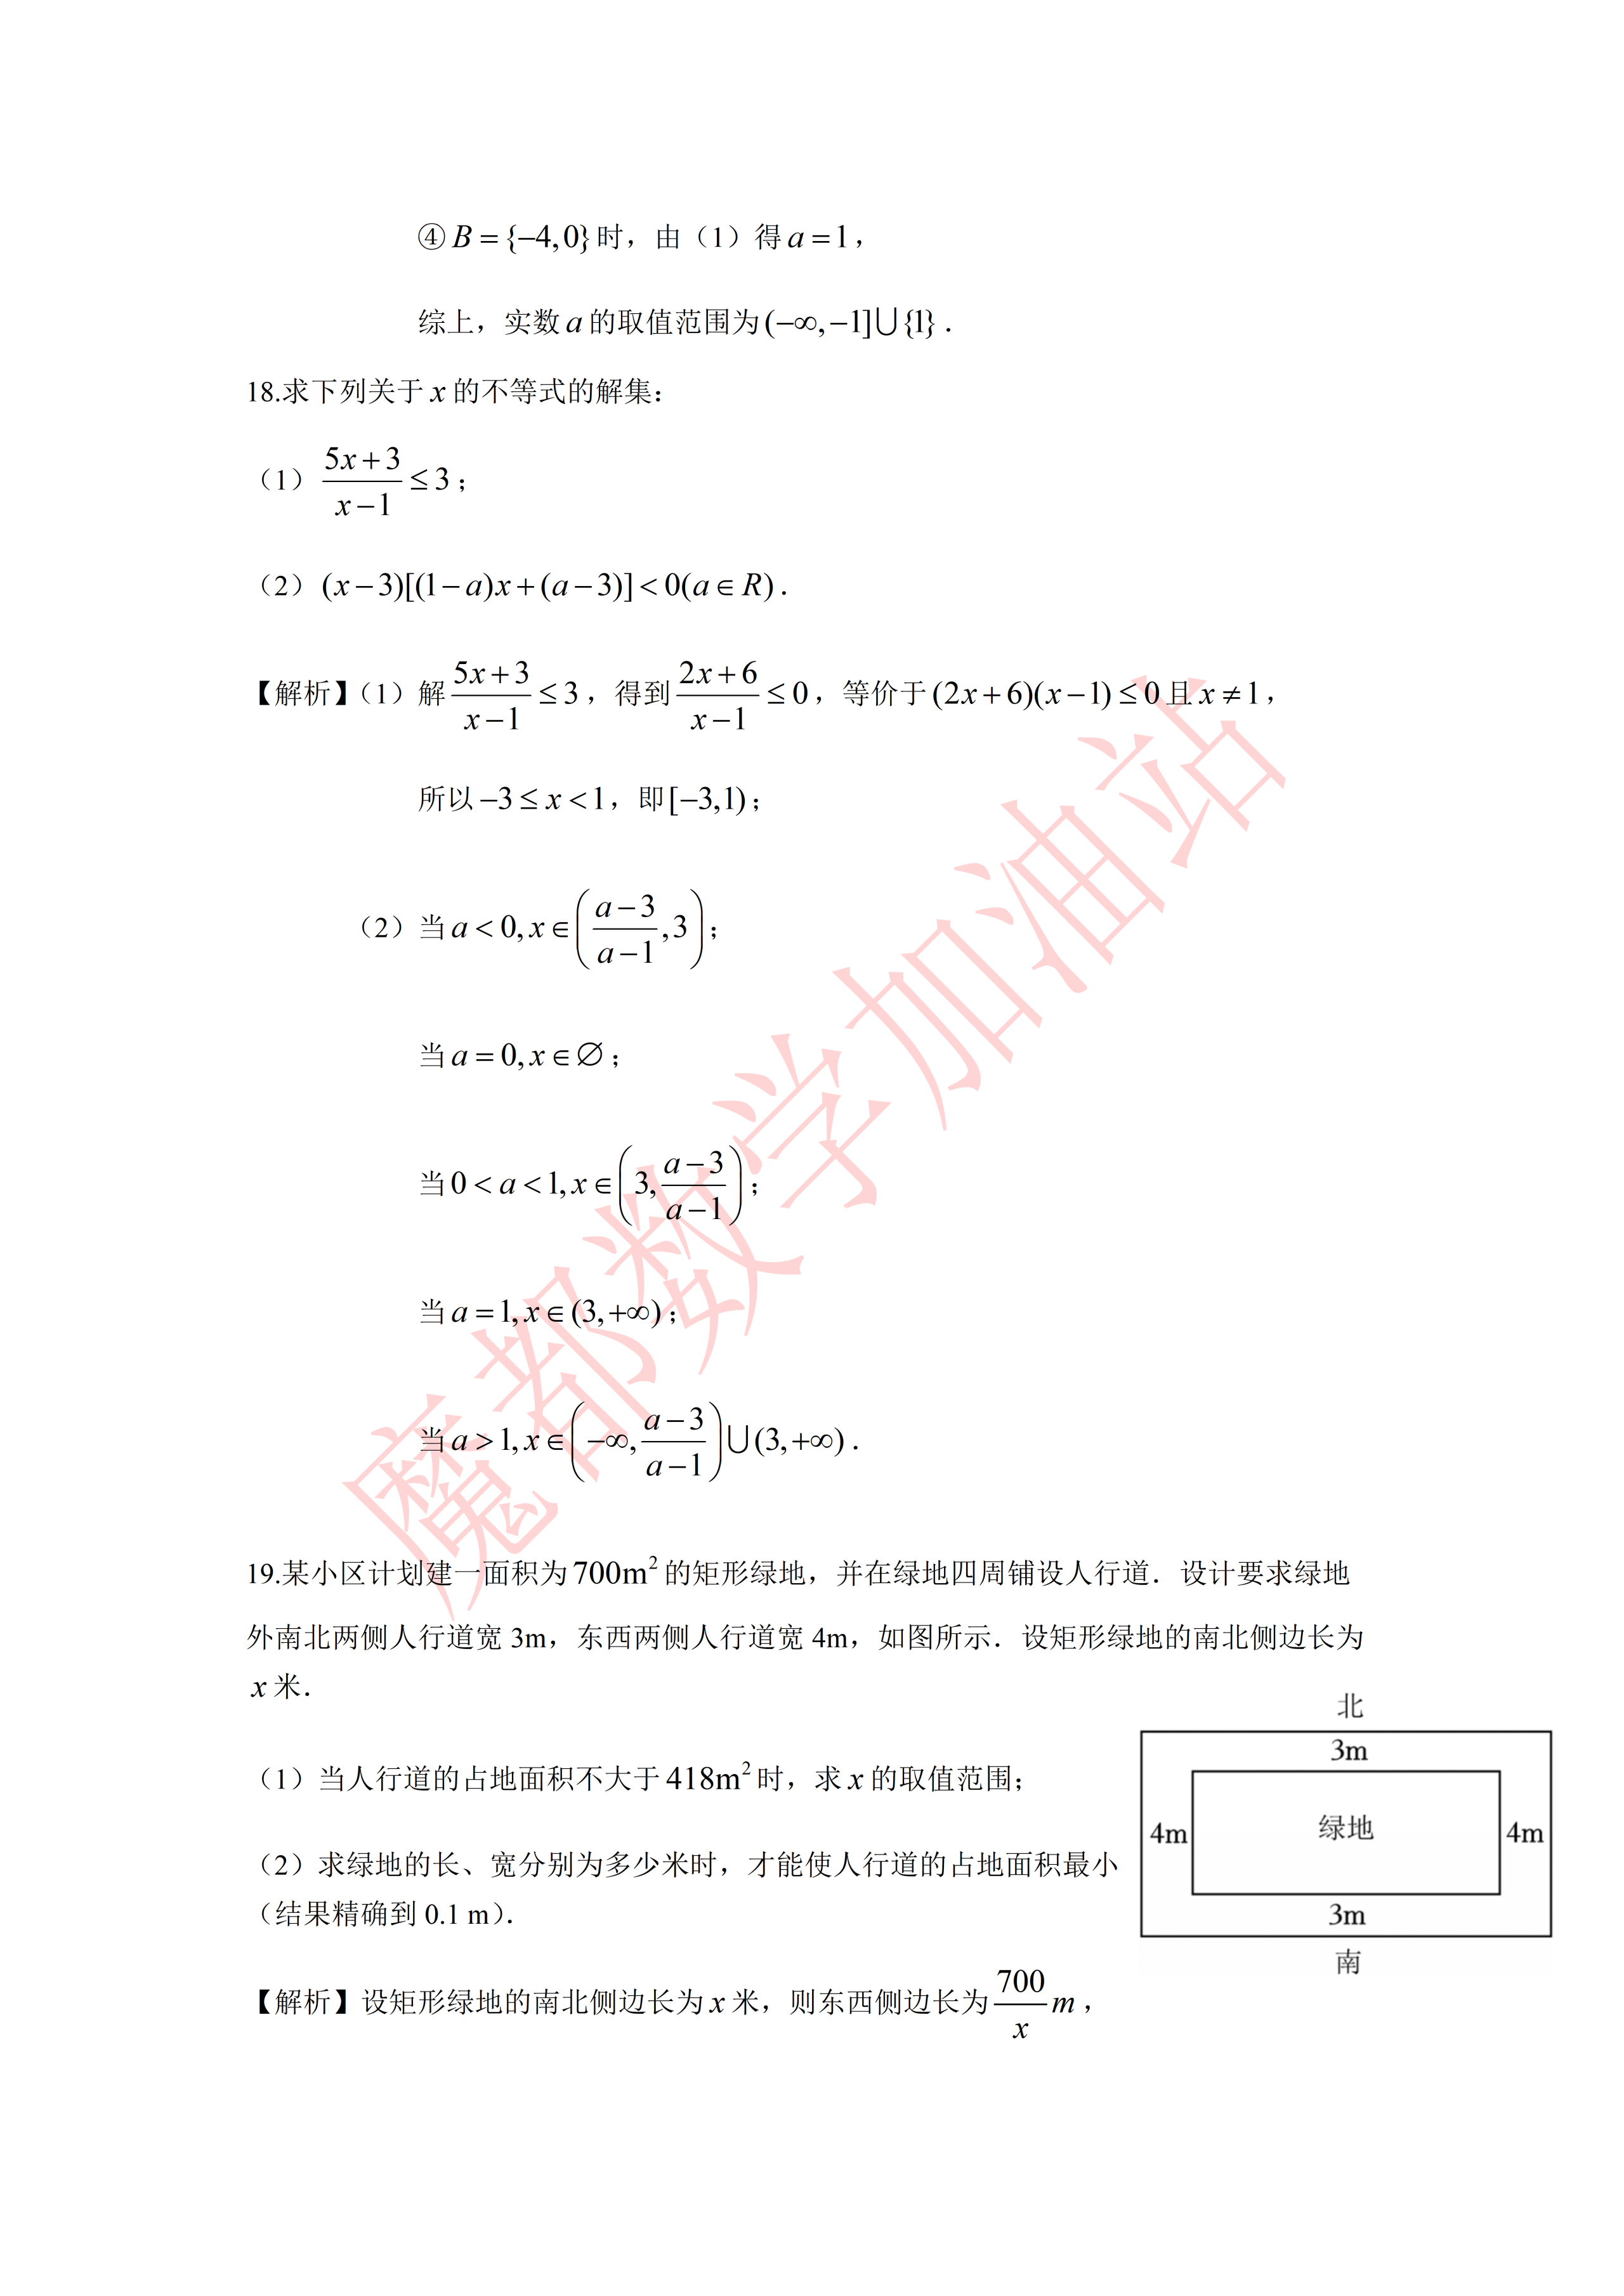
\includegraphics[width=.3\linewidth,trim=1791bp 484bp 107bp 2654bp,clip]{../原图/高一53_华师大二附中_10月月考/07.png}
\end{center}

\begin{enumerate}[label=(\arabic*)]
\item 当人行道的占地面积不大于 $418m^2$ 时，求 $x$ 的取值范围；
\item 求绿地的长、宽分别为多少米时，才能使人行道的占地面积最小（结果精确到 $0.1m$）.
\end{enumerate}

\ifanswer
\solbegin
\step{设矩形绿地的南北侧边长为 $x$ 米，则东西侧边长为 $\dfrac{700}{x}m$，}
\step{则人行道的占地面积为 $S=(x+8)\left(\dfrac{700}{x}+6\right)-700$，即 $S=6x+\dfrac{5600}{x}+48$.}
\stepm{(1)}{当人行道的占地面积不大于 $418m^2$ 时，$6x+\dfrac{5600}{x}+48\leqslant418$，}
\step{即 $6x^2-370x+5600\leqslant0$，解得 $\dfrac{80}{3}\leqslant x\leqslant35$，}
\step{故当人行道的占地面积不大于 $418m^2$ 时，$x\in\left[\dfrac{80}{3},35\right]$；}
\stepm{(2)}{$S=6x+\dfrac{5600}{x}+48\geqslant2\sqrt{6x\cdot\dfrac{5600}{x}}+48=80\sqrt{21}+48$，}
\step{当且仅当 $6x=\dfrac{5600}{x}$，即 $x=20\sqrt{\dfrac73}\approx30.6(m)$ 时，}
% 原卷如此，照录未改（80√21+48≈414.6，两处“414.4”疑笔误，见文件头“原卷笔误/存疑”第 6 条）
\step{$S$ 达到最小值 $80\sqrt{21}+48\approx414.4$，此时 $\dfrac{700}{x}\approx22.9(m)$，}
\step{所以当设计绿地的南北侧边长约为 $30.6m$，东西侧边长约为 $22.9m$ 时，}
\step{人行道的占地面积最小值为 $414.4(m^2)$.}
\solend
\fi

\ansspace[6]

\item 已知 $x\in\R$，符号 $[x]$ 表示不大于 $x$ 的最大整数，例如：$[2.3]=2$,$[2]=2$，$[-1.2]=-2$，令 $S(x)=[x]-[-x]$.

\begin{enumerate}[label=(\arabic*)]
\item 写出 $S(x)$ 为偶数（包括正、负偶数和 0）的充要条件，并证明；
\item 设方程 $|S(x)|=3$ 的解集为 $A$.

①集合 $B=\{x\mid x^2-ax-9\leqslant0,a\in\R\}$，若 $A\cap B=A$，求实数 $a$ 的取值范围；

②集合 $C=\{x\mid 2x^2-5kx+3k^2\geqslant0\}$，若 $A\cup C=\R$，求实数 $k$ 的取值范围.
\end{enumerate}

\ifanswer
\solbegin
\stepm{(1)}{$S(x)$ 为偶数的充要条件是 $x\in\Z$.}
\step{若 $x\in\Z$，则 $S(x)=[x]-[-x]=x-(-x)=2x$；}
\step{若 $x\notin\Z$，设 $[x]=n$，}
\step{则 $S(x)=[x]-[-x]=n-(-n-1)=2n+1=2[x]+1$；}
% 原卷如此，照录未改（“由①”按文意应为“由(1)”，见文件头“原卷笔误/存疑”第 3 条）
\stepm{(2)}{由①得 3 是奇数，$S(x)=\pm3$,$x\notin\Z$，}
\step{$S(x)=2[x]+1=\pm3$,$[x]=1$ 或 $-2$ 且 $x\notin\Z$，}
\step{所以 $A=(-2,-1)\cup(1,2)$；}
\stepm{①}{$A\cap B=A\Rightarrow A\subseteq B$，}
\step{设 $B=[x_1,x_2]$，其中 $x_1,x_2$ 是方程 $x^2-ax-9=0$ 的两实根，}
\step{设 $f(x)=x^2-ax-9$，}
\step{$[-2,2]\subseteq[x_1,x_2]\Leftrightarrow x_1\leqslant-2$,$x_2\geqslant2\Leftrightarrow\begin{cases}f(-2)\leqslant0\\ f(2)\leqslant0\end{cases}$}
\step{$\Leftrightarrow\begin{cases}(-2)^2-a\cdot(-2)-9\leqslant0, & a\leqslant\dfrac52\\ 2^2-2a-9\leqslant0, & a\geqslant-\dfrac52\end{cases}$，故 $a\in\left[-\dfrac52,\dfrac52\right]$；}
\step{注：若用求根公式 $\begin{cases}\dfrac{a+\sqrt{a^2+36}}{2}\geqslant2\Rightarrow a\geqslant-\dfrac52\\ \dfrac{a-\sqrt{a^2+36}}{2}\leqslant-2\Rightarrow a\leqslant\dfrac52\end{cases}$，结果正确，也得满分；}
\stepm{②}{$2x^2-5kx+3k^2=(x-k)(2x-3k)$.}
\step{$A\cup C=\R\Leftrightarrow\complement_\R A\subseteq C$.}
\step{记 $g(x)=2x^2-5kx+3k^2$，则 $\{x\mid g(x)<0\}\subseteq A$.}
\stepm{情况1：}{$k>0$ 时，$k<\dfrac32k$,$g(x)<0$ 的解集为 $\left(k,\dfrac32k\right)\subseteq(1,2)$，}
\step{故 $\begin{cases}k\geqslant1\\ \dfrac32k\leqslant2\end{cases}\Rightarrow1\leqslant k\leqslant\dfrac43$；}
\stepm{情况2：}{$k=0$ 时，$g(x)=2x^2\geqslant0$ 恒成立，$C=\R$,$A\cup C=\R$ 显然成立；}
\stepm{情况3：}{$k<0$ 时，$\dfrac32k<k$,$g(x)<0$ 的解集为 $\left(\dfrac32k,k\right)\subseteq(-2,-1)$，}
\step{故 $\begin{cases}\dfrac32k\geqslant-2\\ k\leqslant-1\end{cases}\Rightarrow-\dfrac43\leqslant k\leqslant-1$；}
\step{综上，$k\in\left[-\dfrac43,-1\right]\cup\{0\}\cup\left[1,\dfrac43\right]$.}
\solend
\fi

\ansspace[10]

\item 对于非空实数集 $M\subseteq(0,+\infty)$，若满足以下两个条件，则称 $M$ 为“极闭集”：

①$M$ 中至少含有 2 个元素，且 $1\notin M$；

②对于 $M$ 中任意两个不相等的元素 $x,y$，定义 $x*y=\dfrac{xy+1}{x+y}$，且 $x*y\in M$.

\begin{enumerate}[label=(\arabic*)]
\item 判断集合 $A=\left\{\dfrac12,2\right\}$ 与区间 $B=(1,+\infty)$ 是否为“极闭集”，并说明理由；
\item 若 $M$ 是“极闭集”，证明：集合 $M$ 中不可能所有元素都小于 1；
\item 证明：不存在任何有限的“极闭集”.
\end{enumerate}

\ifanswer
\solbegin
% 原卷如此，照录未改（首行集合按题干应为 {1/2,2}，见文件头“原卷笔误/存疑”第 7 条）
\stepm{(1)}{对于集合 $A=\left\{\dfrac12,1\right\}$，$\dfrac12*2=\dfrac45$，}
\step{因为 $\dfrac45\notin A$，不满足条件②，所以集合 $A$ 不是“极闭集”.}
\step{对于区间 $B$，满足条件①.}
\step{任取 $B$ 中两个不相等的元素 $x,y$，则 $x>1$,$y>1$.}
\step{$x*y-1=\dfrac{xy+1}{x+y}-1=\dfrac{(x-1)(y-1)}{x+y}>0$，所以 $x*y>1$，}
\step{这说明 $x*y\in B$ 恒成立，满足条件②，所以 $B$ 是“极闭集”.}
\stepm{(2)}{假设集合 $M$ 中所有元素都小于 1，}
\step{在 $M$ 中取 $0<x<y<1$,$x*y-1=\dfrac{xy+1}{x+y}-1=\dfrac{(x-1)(y-1)}{x+y}>0$，}
\step{所以 $x*y>1$，与“集合 $M$ 中所有元素都小于 1”矛盾，}
\step{假设不成立，集合 $M$ 中不可能所有元素都小于 1，得证.}
\stepm{(3)}{由②得，任何一个“极闭集”$M$ 中，必然至少存在一个大于 1 的元素，}
\stepm{情况1：}{若 $M$ 中至少存在两个大于 1 的元素，}
\step{设其中两个不相等的元素为 $x$ 和 $y_1$，且 $x>y_1>1$，}
\step{令 $y_{n+1}=x*y_n$,$n\geqslant1$,$y_{n+1}-1=x*y_n-1=\dfrac{(x-1)(y_n-1)}{xy_n+1}>0$，}
\step{如果 $y_n\geqslant1$，则显然 $y_{n+1}\geqslant1$，作差 $y_n-y_{n+1}=\dfrac{y_n^2-1}{x+y_n}>0$，}
\step{由此 $x>y_1>y_2>y_3>\cdots>1$，与有限集矛盾.}
\stepm{情况2：}{若 $M$ 中恰好只有一个元素大于 1，}
\step{设这个唯一大于 1 的元素为 $m$.}
\step{因为 $M$ 至少有两个元素，所以 $M$ 中必然至少存在一个元素 $a_1<1$，}
\step{令 $a_{n+1}=m*a_n$,$n\geqslant1$，}
\step{又 $a_{n+1}-1=m*a_n-1=\dfrac{(m-1)(a_n-1)}{m+a_n}<0$，故 $a_{n+1}<1$，}
\step{作差 $a_{n+1}-a_n=\dfrac{1-a_n^2}{m+a_n}>0$，由此 $a_1<a_2<a_3<\cdots<1$，与有限集矛盾.}
\step{因此，不存在任何有限的“极闭集”. 原命题得证.}
\solend
\fi

\ansspace*[10]

\end{enumerate}

\end{document}
"
%
% 原始材料：微信公众号“魔都数学加油站”文章，作者破晓，连载“27学年高一53”；
% 原文标题“27学年高一53——2026-2027年上海市华师大二附中高一上10月月考”；
% 原文链接：https://mp.weixin.qq.com/s/fpSnoF-gJEEWyxAoPC_bZA。
% 页面标注发布时间 2026-10-09 17:15（上海）。
% 正文为 11 张 PNG 页：第 01—06、08、10 页 4762×6735，第 07、09、11 页 2560×3620
% （**同一篇各页分辨率不同**），均按页序读取。11 页全为试卷正文页（卷首标题在第 1 页页顶，
% 卷末解答题第 21 题解析止于第 11 页），无封面页、目录页、二维码或宣传页。
% 粉色斜排“魔都数学加油站”为卷面水印，与公众号页脚一并未录入。
%
% 卷首标题：照卷面印作“2026--2027 年华师大二附中高一上 10 月月考”（公众号标题中的“上海市”
% 卷面标题行没有，本稿照卷面），年份区间按全稿惯例排 en dash。原卷只有一行标题、无副标题。
%
% 篇幅与题号：原卷自第 3 题起编号（第 1、2 题不在本卷内）。填空题 3—12（10 题）、
% 选择题 13—16（4 题）、解答题 17—21（5 题），共 19 题。本稿沿用原节与原题号，
% 只改排为全稿统一的大节样式（原卷小节标题为“一、填空题”“二、选择题”“三、解答题”）。
%
% 讲评版：原卷每题下直接印【答案】或【解析】。**第 13 题没有任何【答案】/【解析】段**，
% 答案“C”直接印在题干括号内（“一定不是(  C  )”），本稿按 高一37 第 13 题的成例把括号留空、
% 答案另提为 \ans{$C$}；其余 18 题都只印【解析】，按全稿口径这类题不另提 \ans{}——其中
% 选择题第 14、15、16 题的结论写在解析末句（“故选 B／D／C”），亦照录在解析内。
%
% 副标题：原卷未印副标题。本稿按“知识模块”口径标作“集合与常用逻辑用语、不等式”：
% 19 题中集合与常用逻辑用语 12 题（集合类 9 题——第 4、5、12、13、15、16、17、20、21 题；
% 逻辑类 3 题——第 3、9、14 题），不等式 7 题（含一元二次方程与绝对值方程：第 6、7、8、10、
% 11、18、19 题，其中第 11 题实为奇偶分析下的集合计数题，暂挂不等式），两类均超三分之一，
% 故并标。口径同 高一46、高一47、高一48、高一51、高一52。
%
% 与原卷的排版差异：
%   ① 原卷每题下直接印【解析】，本稿按全稿惯例将答案与解析置于答案版，试卷版保持干净；
%      第 13 题印在题干括号内的答案“C”同样移入 \ans{}，见上；
%   ② 原卷未印副标题，本稿按“知识模块”口径补出；
%   ③ 原卷填空横线约两个字宽，本稿按全稿惯例统一排 \blankline[4.4em]；
%      选择题的作答括号原卷排半角“(    )”，本稿按全稿惯例排 \mbox{（\quad）}；
%   ④ 原卷实数集排斜体/粗体 $R$、$\mathbf{R}$（第 4、6、7、18、20 题等处），本稿按全稿惯例
%      改用 $\R$；空集记号统一为 \varnothing；
%   ⑤ 原卷在数学式内多处用半角逗号（如 $x_1,x_2$、$|S|,|T|$、$a\neq0,c\neq0$），均照录未强改；
%      句末句点按全稿惯例排西文句点（原卷“故选 B．”一类全角句点亦从宽排作“.”）；
%   ⑥ 第 17—21 题的子问原卷各自另起一行，本稿按全稿惯例用 enumerate 的 (1)(2)(3)；
%      第 20 题 (2) 问下的①②两行是题干的一部分，照录为行首①②标号（不入 enumerate）；
%      解析中的子问标号一律用 \stepm{(1)}{…}，解析中的①②③④分情形用 \stepm{①}{…}；
%   ⑦ 第 12、20、21 题解析里的“情况1:”至“情况3:”标号原卷排**红色加粗**（全卷共 6 处），
%      全库无红色排字先例，本稿按全稿子题标号样式排 \stepm{情况1：}{…}（加粗着色、不改黑色基调），
%      冒号照原卷排全角；
%   ⑧ 第 19 题的示意图原卷排在题干右侧（与题干、(1) 问同高），本稿居中排在题干之后、
%      子问之前，并在 \item 前加 \needvspace 整块推走；图自原图第 07 页裁切（trim），不另存图片文件；
%   ⑨ 每道解答题原卷未留作答空白，本稿按全稿惯例加 \ansspace。
%
% 原卷笔误/存疑（均照录未改，正文对应处另有 % 注）：
%   1. 第 14 题解析末行“例如 $a=1$，$b=-1$，及必要性不成立”，“及”按文意应为“即”；
%   2. 第 15 题解析第 3 行 $\dfrac1{a+b\sqrt2}=\dfrac a{a^2-2b}+\left(-\dfrac b{a^2-2b}\right)\cdot\sqrt2$，
%      分母两处均作 $a^2-2b$，按通分应为 $a^2-2b^2$（结论 $C=X$ 不受影响）；
%   3. 第 20 题 (2) 问解析首行“由①得 3 是奇数”，按文意应为“由(1)得”（①是 (2) 问下自己
%      的子问标号，奇偶性结论出自 (1) 问）；
%   4. 第 11 题解析“只有奇数的有 $C_4^2+1=7$ 个”，按组合意义应为 $C_4^2+C_4^4=7$
%      （“$+1$”当指 4 个奇数全取的 1 种），数值无误；
%   5. 第 18 题 (2) 问解析“当 $a=0$,$x\in\varnothing$”，按文意应为“解集为 $\varnothing$”；
%   6. 第 19 题 (2) 问解析“$S$ 达到最小值 $80\sqrt{21}+48\approx414.4$”与末行
%      “人行道的占地面积最小值为 $414.4(m^2)$”，两处按 $80\sqrt{21}+48\approx414.6$，疑笔误；
%   7. 第 21 题 (1) 问解析首行“对于集合 $A=\left\{\frac12,1\right\}$”，按题干应为
%      $A=\left\{\frac12,2\right\}$（计算 $\frac12*2=\frac45$ 用的正是 $2$）；
%   8. 第 12 题解析“所以 $A=(-\infty,-4]\cup[2,+\infty)$”一行行末无标点，体例不一，照录。
%
% 插图：1 张，自原图裁切（无 \begin{tikzpicture} 重排）：
%   · 第 19 题绿地示意图（外矩形内套矩形“绿地”，上“北 3m”、下“南 3m”、左右各“4m”）
%     ——原图第 07 页，原卷排于题干右侧。
%     裁框：x 1797–2447、y 2660–3136（含“北”“南”标注，四周各留约 6px），
%     trim=1791bp 484bp 107bp 2654bp（左／下／右／上），页宽 2560、页高 3620。
%
\documentclass[a4paper,11pt]{article}
\usepackage{common}

\begin{document}

\examtitlest[3]{2026--2027 年华师大二附中高一上 10 月月考}{集合与常用逻辑用语、不等式}

\bigsec{一、填空题}

\begin{enumerate}
\setcounter{enumi}{2}

\item “$x=2$”是“$x^2-3x+2=0$”的\blankline[4.4em]条件.

（选择其中之一填空：充分非必要、必要非充分、充分、既非充分又非必要）

\ifanswer
\solbegin
\step{由 $x^2-3x+2=0$ 得 $x=1$ 或 $x=2$，}
\step{则“$x=2$”是“$x^2-3x+2=0$”的充分不必要条件.}
\solend
\fi

\item 已知 $R$ 是全集，集合 $A=\{y\mid y=-x^2+1,x\in\R\}$，集合 $B=\{x\mid x=3+|a|,a\in\R\}$，则 $\overline{A\cup B}=$\blankline[4.4em].

\ifanswer
\solbegin
\step{$A=\{y\mid y=-x^2+1,x\in\R\}=(-\infty,1]$，$B=\{x\mid x=3+|a|,a\in\R\}=[3,+\infty)$，}
\step{所以 $\overline{A\cup B}=(1,3)$.}
\solend
\fi

\item 已知 $a$ 为常数，集合 $A=\{x\mid x^2+x-6=0\}$，集合 $B=\{x\mid ax-2=0\}$，且 $B\subseteq A$，则 $a$ 的所有取值构成的集合为\blankline[4.4em].

\ifanswer
\solbegin
\step{集合 $A=\{-3,2\}$，因为 $B\subseteq A$，则 $B=\varnothing$，$\{-3\}$，$\{2\}$，$\{-3,2\}$，}
\step{当 $B=\varnothing$ 时，$a=0$，当 $B=\{-3\}$ 时，$a=-\dfrac23$，当 $B=\{2\}$ 时，$a=1$，}
\step{当 $B=\{-3,2\}$ 时，不成立，故 $a$ 的取值集合为 $\left\{0,-\dfrac23,1\right\}$.}
\solend
\fi

\item 设 $a\in\R$，若关于 $x$ 的不等式 $x^2-ax<0$ 的解集是区间 $(0,1)$ 的真子集，则 $a$ 的取值范围是\blankline[4.4em].

\ifanswer
\solbegin
\step{因为关于 $x$ 的不等式 $x^2-ax<0$ 的解集是区间 $(0,1)$ 的真子集，}
\step{当 $a=0$ 时，不等式的解集为 $\varnothing$，符合题意；}
\step{当 $a>0$ 时，不等式的解集为 $(0,a)$，则 $0<a<1$，}
\step{当 $a<0$ 时，不等式的解集为 $(a,0)$，不符合题意，}
\step{故 $a$ 的范围为 $[0,1)$.}
\solend
\fi

\item 设 $x\in\R$，则方程 $|2x+3|-|x-2|=|3x+1|$ 的解集为\blankline[4.4em].

\ifanswer
\solbegin
\step{当 $x\leqslant-\dfrac32$ 时，原式$\Leftrightarrow-2x-3+x-2=-3x-1\Leftrightarrow x=2$，不合题意；}
\step{当 $-\dfrac32<x\leqslant-\dfrac13$ 时，原式$\Leftrightarrow2x+3+x-2=-3x-1\Leftrightarrow x=-\dfrac13$；}
\step{当 $-\dfrac13<x\leqslant2$ 时，原式$\Leftrightarrow2x+3+x-2=3x+1\Leftrightarrow1=1$ 即恒成立；}
\step{当 $x>2$ 时，原式$\Leftrightarrow2x+3+2-x=3x+1\Leftrightarrow x=2$，不合题意；}
\step{故 $x\in\left[-\dfrac13,2\right]$.}
\solend
\fi

\item 已知关于 $x$ 的一元二次方程 $x^2+(4m+1)x+2m-1=0$．若方程的两根为 $x_1$、$x_2$，且满足 $\dfrac1{x_1}+\dfrac1{x_2}=-\dfrac12$，则实数 $m=$\blankline[4.4em].

\ifanswer
\solbegin
\step{由于判别式$\Delta=16m^2+5>0$恒成立，}
\step{不论 $m$ 为任何实数，方程总有两个不相等的实数根.}
\step{$\dfrac1{x_1}+\dfrac1{x_2}=-\dfrac12$，即 $\dfrac{x_1+x_2}{x_1x_2}=-\dfrac12$，由根与系数的关系得 $\dfrac{-4m-1}{2m-1}=-\dfrac12$，}
\step{解得 $m=-\dfrac12$.}
\solend
\fi

\item 已知 $\dfrac1{x-2}\geqslant1$ 是 $|x-a|<2$ 的充分非必要条件，则实数 $a$ 的取值范围是\blankline[4.4em].

\ifanswer
\solbegin
\step{由 $\dfrac1{x-2}\geqslant1$ 得 $\dfrac{3-x}{x-2}\geqslant0$，解得 $2<x\leqslant3$，由 $|x-a|<2$ 得 $a-2<x<a+2$，}
\step{因为 $\dfrac1{x-2}\geqslant1$ 是 $|x-a|<2$ 的充分非必要条件，}
\step{所以 $\{x\mid 2<x\leqslant3\}\subset\{x\mid a-2<x<a+2\}$，所以 $\begin{cases}a-2\leqslant2\\ a+2>3\end{cases}$，解得 $1<a\leqslant4$，}
\step{即实数 $a$ 的取值范围是 $(1,4]$.}
\solend
\fi

\item 设 $x,y\in(0,+\infty)$，且 $x+4y=1$，则 $\dfrac1x+\dfrac1y$ 的最小值为\blankline[4.4em].

\ifanswer
\solbegin
\step{因为 $\dfrac1x+\dfrac1y=(x+4y)\left(\dfrac1x+\dfrac1y\right)=5+\dfrac{4y}{x}+\dfrac{x}{y}\geqslant5+2\sqrt{\dfrac{4y}{x}\cdot\dfrac{x}{y}}=9$，}
\step{当且仅当 $\dfrac{4y}{x}=\dfrac{x}{y}$，即 $x=2y$，即 $x=\dfrac13$,$y=\dfrac16$ 时取等号，故最小值为 $9$.}
\solend
\fi

\item 设非空集合 $Q\subseteq M$，当 $Q$ 中所有元素和为偶数时（集合为单元素时和为元素本身），称 $Q$ 是 $M$ 的偶子集. 若集合 $M=\{1,2,3,4,5,6,7\}$，则其偶子集 $Q$ 的个数为\blankline[4.4em].

\ifanswer
\solbegin
\step{偶子集可以分为只有奇数、偶数及偶数个奇数和偶数的集合，}
\step{奇数有 4 个，偶数有 3 个，}
% 原卷如此，照录未改：按组合意义应为 C_4^2+C_4^4=7（“+1”当指 4 个奇数全取的 1 种），
% 见文件头“原卷笔误/存疑”第 4 条
\step{只有奇数的有 $C_4^2+1=7$ 个，只有偶数的有 $C_3^1+C_3^2+1=7$ 个，}
\step{偶数个奇数和偶数的：两奇一偶 $C_4^2\cdot C_3^1=18$ 个，两奇二偶 $C_4^2\cdot C_3^2=18$ 个，}
\step{两奇三偶 $C_4^2\cdot C_3^3=6$ 个，四奇一偶 $C_4^4\cdot C_3^1=3$ 个，四奇二偶 $C_4^4\cdot C_3^2=3$ 个，}
\step{四奇三偶 $C_4^4\cdot C_3^3=1$ 个，所以共有 $7+7+18+18+6+3+3+1=63$ 个.}
\solend
\fi

\item 已知集合 $A=\{x\mid x^2+2x-8\geqslant0\}$,$B=\{x\mid x^2-2ax+2a\leqslant0\}$，且 $A\cap B$ 中恰有 3 个整数元素，则实数 $a$ 的取值范围为\blankline[4.4em].

\ifanswer
\solbegin
% 原卷如此，照录未改：此行行末无标点，见文件头“原卷笔误/存疑”第 8 条
\step{由 $x^2+2x-8\geqslant0$，得 $x\geqslant2$ 或 $x\leqslant-4$，所以 $A=(-\infty,-4]\cup[2,+\infty)$}
\step{对集合 $B$：$x^2-2ax+2a\leqslant0$,$\Delta=4a^2-8a=4a(a-2)\geqslant0$，}
\step{得 $a\leqslant0$ 或 $a\geqslant2$.}
\step{设方程 $x^2-2ax+2a=0$ 的两根为 $r_1,r_2$，}
\step{则 $B=[r_1,r_2]$,$r_1=a-\sqrt{a^2-2a}$,$r_2=a+\sqrt{a^2-2a}$，}
\stepm{情况1：}{$a\leqslant0$，}
\step{$r_2=a+\sqrt{a^2-2a}<a+\sqrt{a^2-2a+1}=a+|a-1|=a+1-a=1<2$，}
\step{$B$ 只在 $A$ 的左侧部分有交集，要使 $A\cap B$ 恰有 3 个整数元素，}
\step{这 3 个整数为 $-6,-5,-4$，于是 $r_1\in(-7,-6]$，}
\step{令 $f(x)=x^2-2ax+2a$，则 $\begin{cases}f(-7)=49+14a+2a>0\\ f(-6)=36+12a+2a\leqslant0\end{cases}\Rightarrow a\in\left(-\dfrac{49}{16},-\dfrac{18}{7}\right]$；}
\stepm{情况2：}{$a\geqslant2$，}
\step{$r_2=a+\sqrt{a^2-2a}\geqslant2$，}
\step{$r_1=a-\sqrt{a^2-2a}>a-\sqrt{a^2-2a+1}=a-|a-1|=a-(a-1)=1>-4$，}
\step{所以 $A\cap B=[2,r_2]$.}
\step{同理 $\begin{cases}f(4)=16-8a+2a\leqslant0\\ f(5)=25-10a+2a>0\end{cases}\Rightarrow a\in\left[\dfrac{8}{3},\dfrac{25}{8}\right)$；}
\step{综上，$a\in\left(-\dfrac{49}{16},-\dfrac{18}{7}\right]\cup\left[\dfrac{8}{3},\dfrac{25}{8}\right)$.}
\solend
\fi

\end{enumerate}

\bigsec{二、选择题}

\begin{enumerate}
\setcounter{enumi}{12}

% 第 13 题原卷无【答案】/【解析】段，答案“C”直接印在题干括号内，
% 按高一37 第 13 题的成例括号留空、答案另提为 \ans{}（见文件头）
\item 集合 $A=\{a,b,c\}$ 中的三个元素分别表示某一个三角形的三边长度，那么这个三角形一定不是\mbox{（\quad）}

\keepwithprev
A. 锐角三角形\qquad B. 钝角三角形

C. 等腰三角形\qquad D. 直角三角形

\ifanswer
\ans{$C$}
\fi

\item 设 $a$、$b$ 为实数，则“$a<b<0$”是“$\dfrac1a>\dfrac1b$”的\mbox{（\quad）}条件.

\keepwithprev
A. 充要\qquad B. 充分不必要

C. 必要不充分\qquad D. 既不充分也不必要

\ifanswer
\solbegin
\step{若 $a<b<0$，则 $\dfrac1a>\dfrac1b$ 一定成立，即充分性成立；}
% 原卷如此，照录未改（“及”按文意应为“即”，见文件头“原卷笔误/存疑”第 1 条）
\step{若 $\dfrac1a>\dfrac1b$ 成立，$a<b<0$ 不一定成立，例如 $a=1$，$b=-1$，及必要性不成立.}
\step{故选 $B$.}
\solend
\fi

\item 设 $Q$ 表示有理数集，集合 $X=\{x\mid x=a+b\sqrt2,a,b\in Q,x\neq0\}$，在下列集合中：①$\{2x\mid x\in X\}$②$\left\{\dfrac{x}{\sqrt2}\mid x\in X\right\}$③$\left\{\dfrac1x\mid x\in X\right\}$④$\{x^2\mid x\in X\}$，与 $X$ 相同的集合有\mbox{（\quad）}

\keepwithprev
A. ①②③④\qquad B. ②③④\qquad C. ①②④\qquad D. ①②③

\ifanswer
\solbegin
\step{$A=\{2x\mid x\in X\}$，$2(a+b\sqrt2)=p+q\sqrt2$ 得 $p=2a$，$q=2b$，$a=\dfrac p2$，$b=\dfrac q2$，}
\step{也是一一对应，$A=X$}
% 原卷如此，照录未改：分母两处均作 a^2-2b，按通分应为 a^2-2b^2，
% 见文件头“原卷笔误/存疑”第 2 条
\step{集合 $B=\left\{\dfrac{x}{\sqrt2}\mid x\in X\right\}$，$\dfrac{a+b\sqrt2}{\sqrt2}=b+\dfrac a2\cdot\sqrt2$，也是一一对应，$B=X$}
\step{集合 $C=\left\{\dfrac1x\mid x\in X\right\}$，$\dfrac{1}{a+b\sqrt2}=\dfrac{a}{a^2-2b}+\left(-\dfrac{b}{a^2-2b}\right)\cdot\sqrt2$，一一对应，$C=X$}
\step{集合 $D=\{x^2\mid x\in X\}$，$(a+b\sqrt2)^2=a^2+2b^2+2ab\sqrt2$，这个不能一一对应了，}
\step{集合 $D$ 包含于 $X$ 中.}
\step{故 $X$ 相同的集合有①②③，故选 $D$.}
\solend
\fi

\item 集合 $S=\{x\mid(x+a)(x^2+bx+c)=0\}$,$T=\{x\mid(ax+1)(cx^2+bx+1)=0\}$，其中 $a,b,c$ 为实数，若 $|S|,|T|$ 分别表示集合 $S,T$ 的元素个数，则 $|S|-|T|$ 的所有可能取值集合为\mbox{（\quad）}

\keepwithprev
A. $\{0\}$\qquad B. $\{1\}$\qquad C. $\{0,1\}$\qquad D. $\{-1,0,1\}$

\ifanswer
\solbegin
\stepm{①}{$a\neq0,c\neq0$ 时.}
\step{$S$ 中 $x+a=0$ 的根 $x=-a$;$T$ 中 $ax+1=0$ 的根 $x=-\dfrac1a$.}
\step{$S$ 中的 $x^2+bx+c=0$ 若无实根，则 $T$ 中的 $cx^2+bx+1=0$ 也无实根；}
\step{又设 $S$ 的 $x^2+bx+c=0$ 的根为 $r(r\neq0)$，则 $T$ 的 $cx^2+bx+1=0$ 的根为 $\dfrac1r$.}
\step{（因为 $r^2+br+c=0\Rightarrow c\cdot\left(\dfrac1r\right)^2+b\cdot\dfrac1r+1=0$）}
\step{即 $a\neq0,c\neq0$ 时，}
\step{$S$ 与 $T$ 的实根存在一一对应关系 $x\leftrightarrow\dfrac1x$,$|S|=|T|,$$|S|-|T|=0$；}
\stepm{②}{$a=0,c\neq0$ 时.}
\step{$S$ 中多出一个根 $x=0$，而 $T$ 中无此根，$|S|=|T|+1$，即 $|S|-|T|=1$；}
\stepm{③}{$a\neq0,c=0$ 时.}
\step{则 $S$ 中仍有根 $x=0$，而 $T$ 中无 0 根，同样 $|S|-|T|=1$.}
\stepm{④}{$a=0,c=0$ 时.}
\step{同样 $S$ 含有根 0，而 $T$ 中不含 0，仍有 $|S|-|T|=1$.}
\step{综上，$|S|-|T|$ 所有可能取值为 0 和 1，故选 $C$.}
\solend
\fi

\end{enumerate}

\bigsec{三、解答题}

\begin{enumerate}
\setcounter{enumi}{16}

\item 已知集合 $A=\{x\mid x^2+4x=0\}$，$B=\{x\mid x^2+2(a+1)x+a^2-1=0\}$.

\begin{enumerate}[label=(\arabic*)]
\item 若 $A$ 是 $B$ 的子集，求实数 $a$ 的值；
\item 若 $B$ 是 $A$ 的子集，求实数 $a$ 的取值范围.
\end{enumerate}

\ifanswer
\solbegin
\stepm{(1)}{因为 $A=\{-4,0\}$，$B=\{x\mid x^2+2(a+1)x+a^2-1=0\}$，又 $A\subseteq B$，}
\step{所以 $A=B$，所以 $\begin{cases}-4+0=-2(a+1)\\ -4\times0=a^2-1\end{cases}$，所以 $a=1$；}
\stepm{(2)}{因为 $B$ 是 $A$ 的子集，所以 $B=\varnothing$ 或 $B=\{-4\}$ 或 $B=\{0\}$ 或 $B=\{-4,0\}$，}
\stepm{①}{$B=\varnothing$ 时，$\Delta=4(a+1)^2-4(a^2-1)<0$，所以 $a<-1$；}
\stepm{②}{$B=\{-4\}$ 时，$\begin{cases}-4+(-4)=-2(a+1)\\ -4\times(-4)=a^2-1\end{cases}$，无解；}
\stepm{③}{$B=\{0\}$ 时，$\begin{cases}0+0=-2(a+1)\\ 0\times0=a^2-1\end{cases}$，所以 $a=-1$；}
\stepm{④}{$B=\{-4,0\}$ 时，由（1）得 $a=1$，}
\step{综上，实数 $a$ 的取值范围为 $(-\infty,-1]\cup\{1\}$.}
\solend
\fi

\ansspace[6]

\item 求下列关于 $x$ 的不等式的解集：

\begin{enumerate}[label=(\arabic*)]
\item $\dfrac{5x+3}{x-1}\leqslant3$；
\item $(x-3)[(1-a)x+(a-3)]<0$ ($a\in\R$).
\end{enumerate}

\ifanswer
\solbegin
\stepm{(1)}{解 $\dfrac{5x+3}{x-1}\leqslant3$，得到 $\dfrac{2x+6}{x-1}\leqslant0$，等价于 $(2x+6)(x-1)\leqslant0$ 且 $x\neq1$，}
\step{所以 $-3\leqslant x<1$，即 $[-3,1)$；}
\stepm{(2)}{当 $a<0$,$x\in\left(\dfrac{a-3}{a-1},3\right)$；}
% 原卷如此，照录未改（“x∈∅”按文意应为“解集为 ∅”，见文件头“原卷笔误/存疑”第 5 条）
\step{当 $a=0$,$x\in\varnothing$；}
\step{当 $0<a<1$,$x\in\left(3,\dfrac{a-3}{a-1}\right)$；}
\step{当 $a=1$,$x\in(3,+\infty)$；}
\step{当 $a>1$,$x\in\left(-\infty,\dfrac{a-3}{a-1}\right)\cup(3,+\infty)$.}
\solend
\fi

\ansspace[6]

\needvspace{13\baselineskip}

\item 某小区计划建一面积为 $700m^2$ 的矩形绿地，并在绿地四周铺设人行道. 设计要求绿地外南北两侧人行道宽 $3m$，东西两侧人行道宽 $4m$，如图所示. 设矩形绿地的南北侧边长为 $x$ 米.

\begin{center}
% 原图第 7 页题干绿地示意图直接裁取（原卷排于题干右侧）。
% 裁框取图形外框 x 1797–2447、y 2660–3136（含“北”“南”标注，四周各留约 6px），
% trim=左 1791bp／下 484bp／右 107bp／上 2654bp（页宽 2560、页高 3620）。
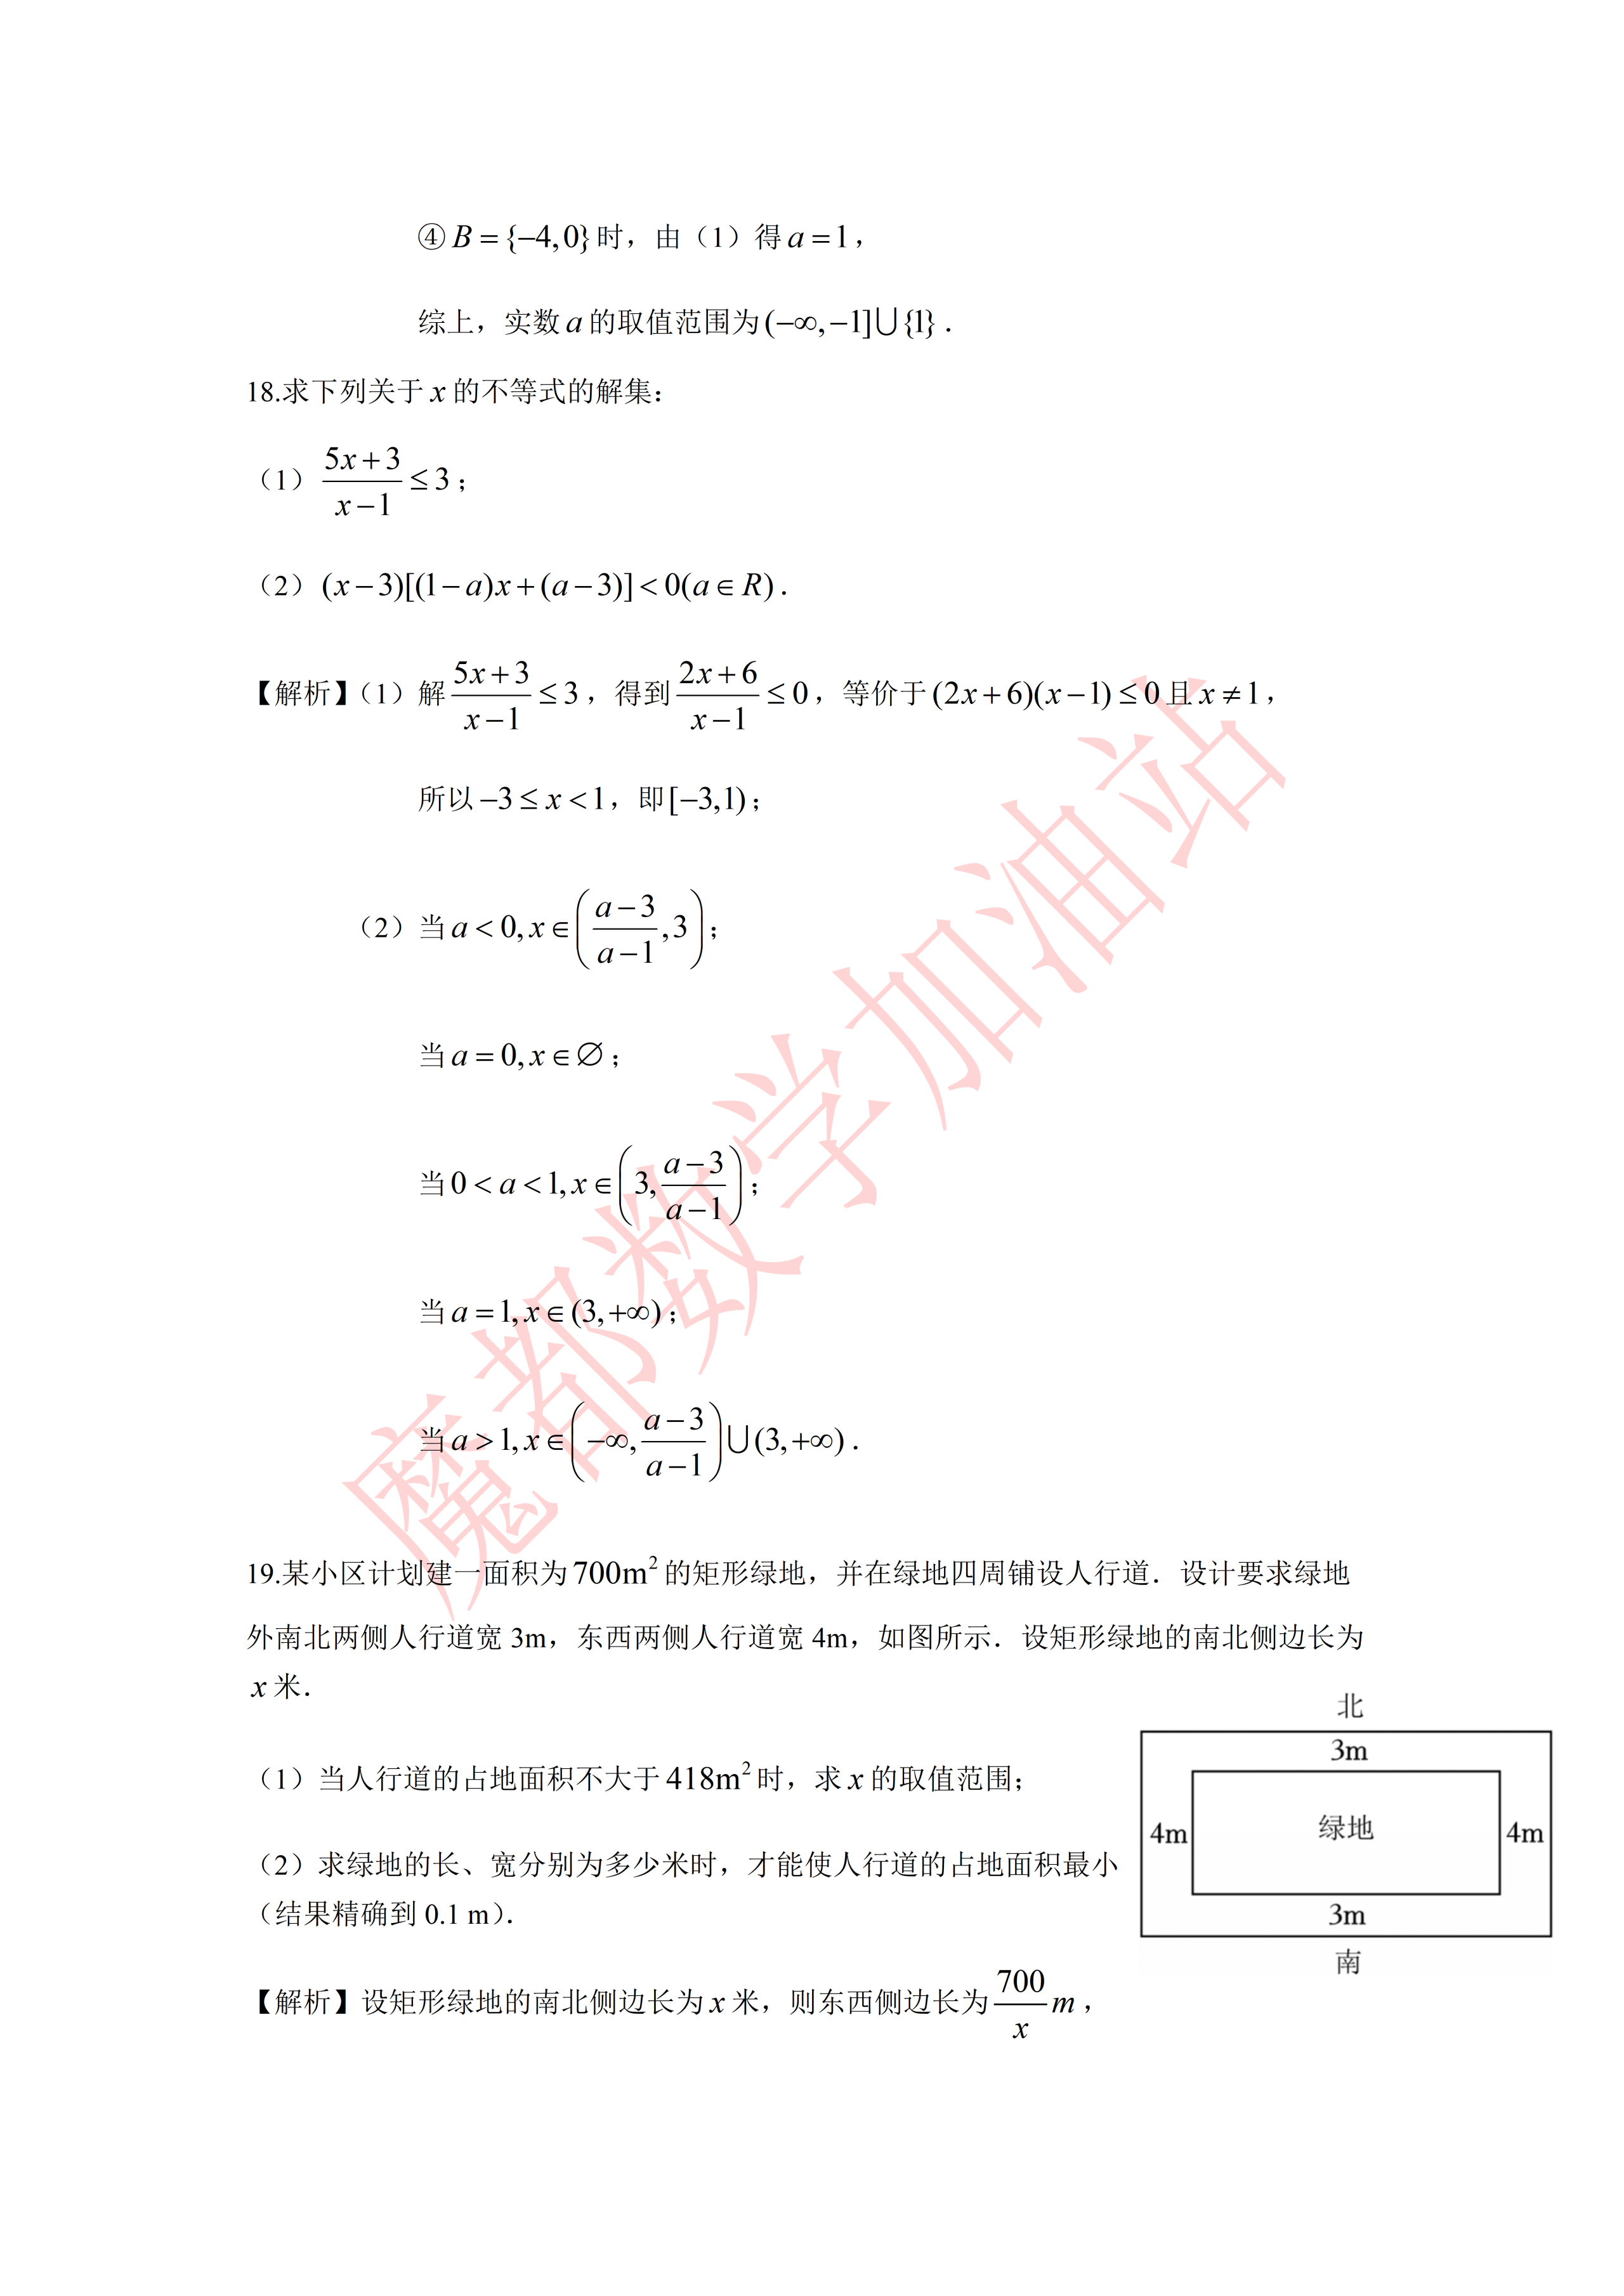
\includegraphics[width=.3\linewidth,trim=1791bp 484bp 107bp 2654bp,clip]{../原图/高一53_华师大二附中_10月月考/07.png}
\end{center}

\begin{enumerate}[label=(\arabic*)]
\item 当人行道的占地面积不大于 $418m^2$ 时，求 $x$ 的取值范围；
\item 求绿地的长、宽分别为多少米时，才能使人行道的占地面积最小（结果精确到 $0.1m$）.
\end{enumerate}

\ifanswer
\solbegin
\step{设矩形绿地的南北侧边长为 $x$ 米，则东西侧边长为 $\dfrac{700}{x}m$，}
\step{则人行道的占地面积为 $S=(x+8)\left(\dfrac{700}{x}+6\right)-700$，即 $S=6x+\dfrac{5600}{x}+48$.}
\stepm{(1)}{当人行道的占地面积不大于 $418m^2$ 时，$6x+\dfrac{5600}{x}+48\leqslant418$，}
\step{即 $6x^2-370x+5600\leqslant0$，解得 $\dfrac{80}{3}\leqslant x\leqslant35$，}
\step{故当人行道的占地面积不大于 $418m^2$ 时，$x\in\left[\dfrac{80}{3},35\right]$；}
\stepm{(2)}{$S=6x+\dfrac{5600}{x}+48\geqslant2\sqrt{6x\cdot\dfrac{5600}{x}}+48=80\sqrt{21}+48$，}
\step{当且仅当 $6x=\dfrac{5600}{x}$，即 $x=20\sqrt{\dfrac73}\approx30.6(m)$ 时，}
% 原卷如此，照录未改（80√21+48≈414.6，两处“414.4”疑笔误，见文件头“原卷笔误/存疑”第 6 条）
\step{$S$ 达到最小值 $80\sqrt{21}+48\approx414.4$，此时 $\dfrac{700}{x}\approx22.9(m)$，}
\step{所以当设计绿地的南北侧边长约为 $30.6m$，东西侧边长约为 $22.9m$ 时，}
\step{人行道的占地面积最小值为 $414.4(m^2)$.}
\solend
\fi

\ansspace[6]

\item 已知 $x\in\R$，符号 $[x]$ 表示不大于 $x$ 的最大整数，例如：$[2.3]=2$,$[2]=2$，$[-1.2]=-2$，令 $S(x)=[x]-[-x]$.

\begin{enumerate}[label=(\arabic*)]
\item 写出 $S(x)$ 为偶数（包括正、负偶数和 0）的充要条件，并证明；
\item 设方程 $|S(x)|=3$ 的解集为 $A$.

①集合 $B=\{x\mid x^2-ax-9\leqslant0,a\in\R\}$，若 $A\cap B=A$，求实数 $a$ 的取值范围；

②集合 $C=\{x\mid 2x^2-5kx+3k^2\geqslant0\}$，若 $A\cup C=\R$，求实数 $k$ 的取值范围.
\end{enumerate}

\ifanswer
\solbegin
\stepm{(1)}{$S(x)$ 为偶数的充要条件是 $x\in\Z$.}
\step{若 $x\in\Z$，则 $S(x)=[x]-[-x]=x-(-x)=2x$；}
\step{若 $x\notin\Z$，设 $[x]=n$，}
\step{则 $S(x)=[x]-[-x]=n-(-n-1)=2n+1=2[x]+1$；}
% 原卷如此，照录未改（“由①”按文意应为“由(1)”，见文件头“原卷笔误/存疑”第 3 条）
\stepm{(2)}{由①得 3 是奇数，$S(x)=\pm3$,$x\notin\Z$，}
\step{$S(x)=2[x]+1=\pm3$,$[x]=1$ 或 $-2$ 且 $x\notin\Z$，}
\step{所以 $A=(-2,-1)\cup(1,2)$；}
\stepm{①}{$A\cap B=A\Rightarrow A\subseteq B$，}
\step{设 $B=[x_1,x_2]$，其中 $x_1,x_2$ 是方程 $x^2-ax-9=0$ 的两实根，}
\step{设 $f(x)=x^2-ax-9$，}
\step{$[-2,2]\subseteq[x_1,x_2]\Leftrightarrow x_1\leqslant-2$,$x_2\geqslant2\Leftrightarrow\begin{cases}f(-2)\leqslant0\\ f(2)\leqslant0\end{cases}$}
\step{$\Leftrightarrow\begin{cases}(-2)^2-a\cdot(-2)-9\leqslant0, & a\leqslant\dfrac52\\ 2^2-2a-9\leqslant0, & a\geqslant-\dfrac52\end{cases}$，故 $a\in\left[-\dfrac52,\dfrac52\right]$；}
\step{注：若用求根公式 $\begin{cases}\dfrac{a+\sqrt{a^2+36}}{2}\geqslant2\Rightarrow a\geqslant-\dfrac52\\ \dfrac{a-\sqrt{a^2+36}}{2}\leqslant-2\Rightarrow a\leqslant\dfrac52\end{cases}$，结果正确，也得满分；}
\stepm{②}{$2x^2-5kx+3k^2=(x-k)(2x-3k)$.}
\step{$A\cup C=\R\Leftrightarrow\complement_\R A\subseteq C$.}
\step{记 $g(x)=2x^2-5kx+3k^2$，则 $\{x\mid g(x)<0\}\subseteq A$.}
\stepm{情况1：}{$k>0$ 时，$k<\dfrac32k$,$g(x)<0$ 的解集为 $\left(k,\dfrac32k\right)\subseteq(1,2)$，}
\step{故 $\begin{cases}k\geqslant1\\ \dfrac32k\leqslant2\end{cases}\Rightarrow1\leqslant k\leqslant\dfrac43$；}
\stepm{情况2：}{$k=0$ 时，$g(x)=2x^2\geqslant0$ 恒成立，$C=\R$,$A\cup C=\R$ 显然成立；}
\stepm{情况3：}{$k<0$ 时，$\dfrac32k<k$,$g(x)<0$ 的解集为 $\left(\dfrac32k,k\right)\subseteq(-2,-1)$，}
\step{故 $\begin{cases}\dfrac32k\geqslant-2\\ k\leqslant-1\end{cases}\Rightarrow-\dfrac43\leqslant k\leqslant-1$；}
\step{综上，$k\in\left[-\dfrac43,-1\right]\cup\{0\}\cup\left[1,\dfrac43\right]$.}
\solend
\fi

\ansspace[10]

\item 对于非空实数集 $M\subseteq(0,+\infty)$，若满足以下两个条件，则称 $M$ 为“极闭集”：

①$M$ 中至少含有 2 个元素，且 $1\notin M$；

②对于 $M$ 中任意两个不相等的元素 $x,y$，定义 $x*y=\dfrac{xy+1}{x+y}$，且 $x*y\in M$.

\begin{enumerate}[label=(\arabic*)]
\item 判断集合 $A=\left\{\dfrac12,2\right\}$ 与区间 $B=(1,+\infty)$ 是否为“极闭集”，并说明理由；
\item 若 $M$ 是“极闭集”，证明：集合 $M$ 中不可能所有元素都小于 1；
\item 证明：不存在任何有限的“极闭集”.
\end{enumerate}

\ifanswer
\solbegin
% 原卷如此，照录未改（首行集合按题干应为 {1/2,2}，见文件头“原卷笔误/存疑”第 7 条）
\stepm{(1)}{对于集合 $A=\left\{\dfrac12,1\right\}$，$\dfrac12*2=\dfrac45$，}
\step{因为 $\dfrac45\notin A$，不满足条件②，所以集合 $A$ 不是“极闭集”.}
\step{对于区间 $B$，满足条件①.}
\step{任取 $B$ 中两个不相等的元素 $x,y$，则 $x>1$,$y>1$.}
\step{$x*y-1=\dfrac{xy+1}{x+y}-1=\dfrac{(x-1)(y-1)}{x+y}>0$，所以 $x*y>1$，}
\step{这说明 $x*y\in B$ 恒成立，满足条件②，所以 $B$ 是“极闭集”.}
\stepm{(2)}{假设集合 $M$ 中所有元素都小于 1，}
\step{在 $M$ 中取 $0<x<y<1$,$x*y-1=\dfrac{xy+1}{x+y}-1=\dfrac{(x-1)(y-1)}{x+y}>0$，}
\step{所以 $x*y>1$，与“集合 $M$ 中所有元素都小于 1”矛盾，}
\step{假设不成立，集合 $M$ 中不可能所有元素都小于 1，得证.}
\stepm{(3)}{由②得，任何一个“极闭集”$M$ 中，必然至少存在一个大于 1 的元素，}
\stepm{情况1：}{若 $M$ 中至少存在两个大于 1 的元素，}
\step{设其中两个不相等的元素为 $x$ 和 $y_1$，且 $x>y_1>1$，}
\step{令 $y_{n+1}=x*y_n$,$n\geqslant1$,$y_{n+1}-1=x*y_n-1=\dfrac{(x-1)(y_n-1)}{xy_n+1}>0$，}
\step{如果 $y_n\geqslant1$，则显然 $y_{n+1}\geqslant1$，作差 $y_n-y_{n+1}=\dfrac{y_n^2-1}{x+y_n}>0$，}
\step{由此 $x>y_1>y_2>y_3>\cdots>1$，与有限集矛盾.}
\stepm{情况2：}{若 $M$ 中恰好只有一个元素大于 1，}
\step{设这个唯一大于 1 的元素为 $m$.}
\step{因为 $M$ 至少有两个元素，所以 $M$ 中必然至少存在一个元素 $a_1<1$，}
\step{令 $a_{n+1}=m*a_n$,$n\geqslant1$，}
\step{又 $a_{n+1}-1=m*a_n-1=\dfrac{(m-1)(a_n-1)}{m+a_n}<0$，故 $a_{n+1}<1$，}
\step{作差 $a_{n+1}-a_n=\dfrac{1-a_n^2}{m+a_n}>0$，由此 $a_1<a_2<a_3<\cdots<1$，与有限集矛盾.}
\step{因此，不存在任何有限的“极闭集”. 原命题得证.}
\solend
\fi

\ansspace*[10]

\end{enumerate}

\end{document}
"
% 紧凑版：xelatex "\def\iscompact{1}% 高一53_华师大二附中_10月月考.tex
%   —— 高一上数学“2026-2027 年华师大二附中高一上 10 月月考”（讲评版）
% 试卷版：xelatex 高一53_华师大二附中_10月月考.tex
% 答案版：xelatex "\def\isanswer{1}% 高一53_华师大二附中_10月月考.tex
%   —— 高一上数学“2026-2027 年华师大二附中高一上 10 月月考”（讲评版）
% 试卷版：xelatex 高一53_华师大二附中_10月月考.tex
% 答案版：xelatex "\def\isanswer{1}% 高一53_华师大二附中_10月月考.tex
%   —— 高一上数学“2026-2027 年华师大二附中高一上 10 月月考”（讲评版）
% 试卷版：xelatex 高一53_华师大二附中_10月月考.tex
% 答案版：xelatex "\def\isanswer{1}\input{高一53_华师大二附中_10月月考.tex}"
% 紧凑版：xelatex "\def\iscompact{1}\input{高一53_华师大二附中_10月月考.tex}"
%
% 原始材料：微信公众号“魔都数学加油站”文章，作者破晓，连载“27学年高一53”；
% 原文标题“27学年高一53——2026-2027年上海市华师大二附中高一上10月月考”；
% 原文链接：https://mp.weixin.qq.com/s/fpSnoF-gJEEWyxAoPC_bZA。
% 页面标注发布时间 2026-10-09 17:15（上海）。
% 正文为 11 张 PNG 页：第 01—06、08、10 页 4762×6735，第 07、09、11 页 2560×3620
% （**同一篇各页分辨率不同**），均按页序读取。11 页全为试卷正文页（卷首标题在第 1 页页顶，
% 卷末解答题第 21 题解析止于第 11 页），无封面页、目录页、二维码或宣传页。
% 粉色斜排“魔都数学加油站”为卷面水印，与公众号页脚一并未录入。
%
% 卷首标题：照卷面印作“2026--2027 年华师大二附中高一上 10 月月考”（公众号标题中的“上海市”
% 卷面标题行没有，本稿照卷面），年份区间按全稿惯例排 en dash。原卷只有一行标题、无副标题。
%
% 篇幅与题号：原卷自第 3 题起编号（第 1、2 题不在本卷内）。填空题 3—12（10 题）、
% 选择题 13—16（4 题）、解答题 17—21（5 题），共 19 题。本稿沿用原节与原题号，
% 只改排为全稿统一的大节样式（原卷小节标题为“一、填空题”“二、选择题”“三、解答题”）。
%
% 讲评版：原卷每题下直接印【答案】或【解析】。**第 13 题没有任何【答案】/【解析】段**，
% 答案“C”直接印在题干括号内（“一定不是(  C  )”），本稿按 高一37 第 13 题的成例把括号留空、
% 答案另提为 \ans{$C$}；其余 18 题都只印【解析】，按全稿口径这类题不另提 \ans{}——其中
% 选择题第 14、15、16 题的结论写在解析末句（“故选 B／D／C”），亦照录在解析内。
%
% 副标题：原卷未印副标题。本稿按“知识模块”口径标作“集合与常用逻辑用语、不等式”：
% 19 题中集合与常用逻辑用语 12 题（集合类 9 题——第 4、5、12、13、15、16、17、20、21 题；
% 逻辑类 3 题——第 3、9、14 题），不等式 7 题（含一元二次方程与绝对值方程：第 6、7、8、10、
% 11、18、19 题，其中第 11 题实为奇偶分析下的集合计数题，暂挂不等式），两类均超三分之一，
% 故并标。口径同 高一46、高一47、高一48、高一51、高一52。
%
% 与原卷的排版差异：
%   ① 原卷每题下直接印【解析】，本稿按全稿惯例将答案与解析置于答案版，试卷版保持干净；
%      第 13 题印在题干括号内的答案“C”同样移入 \ans{}，见上；
%   ② 原卷未印副标题，本稿按“知识模块”口径补出；
%   ③ 原卷填空横线约两个字宽，本稿按全稿惯例统一排 \blankline[4.4em]；
%      选择题的作答括号原卷排半角“(    )”，本稿按全稿惯例排 \mbox{（\quad）}；
%   ④ 原卷实数集排斜体/粗体 $R$、$\mathbf{R}$（第 4、6、7、18、20 题等处），本稿按全稿惯例
%      改用 $\R$；空集记号统一为 \varnothing；
%   ⑤ 原卷在数学式内多处用半角逗号（如 $x_1,x_2$、$|S|,|T|$、$a\neq0,c\neq0$），均照录未强改；
%      句末句点按全稿惯例排西文句点（原卷“故选 B．”一类全角句点亦从宽排作“.”）；
%   ⑥ 第 17—21 题的子问原卷各自另起一行，本稿按全稿惯例用 enumerate 的 (1)(2)(3)；
%      第 20 题 (2) 问下的①②两行是题干的一部分，照录为行首①②标号（不入 enumerate）；
%      解析中的子问标号一律用 \stepm{(1)}{…}，解析中的①②③④分情形用 \stepm{①}{…}；
%   ⑦ 第 12、20、21 题解析里的“情况1:”至“情况3:”标号原卷排**红色加粗**（全卷共 6 处），
%      全库无红色排字先例，本稿按全稿子题标号样式排 \stepm{情况1：}{…}（加粗着色、不改黑色基调），
%      冒号照原卷排全角；
%   ⑧ 第 19 题的示意图原卷排在题干右侧（与题干、(1) 问同高），本稿居中排在题干之后、
%      子问之前，并在 \item 前加 \needvspace 整块推走；图自原图第 07 页裁切（trim），不另存图片文件；
%   ⑨ 每道解答题原卷未留作答空白，本稿按全稿惯例加 \ansspace。
%
% 原卷笔误/存疑（均照录未改，正文对应处另有 % 注）：
%   1. 第 14 题解析末行“例如 $a=1$，$b=-1$，及必要性不成立”，“及”按文意应为“即”；
%   2. 第 15 题解析第 3 行 $\dfrac1{a+b\sqrt2}=\dfrac a{a^2-2b}+\left(-\dfrac b{a^2-2b}\right)\cdot\sqrt2$，
%      分母两处均作 $a^2-2b$，按通分应为 $a^2-2b^2$（结论 $C=X$ 不受影响）；
%   3. 第 20 题 (2) 问解析首行“由①得 3 是奇数”，按文意应为“由(1)得”（①是 (2) 问下自己
%      的子问标号，奇偶性结论出自 (1) 问）；
%   4. 第 11 题解析“只有奇数的有 $C_4^2+1=7$ 个”，按组合意义应为 $C_4^2+C_4^4=7$
%      （“$+1$”当指 4 个奇数全取的 1 种），数值无误；
%   5. 第 18 题 (2) 问解析“当 $a=0$,$x\in\varnothing$”，按文意应为“解集为 $\varnothing$”；
%   6. 第 19 题 (2) 问解析“$S$ 达到最小值 $80\sqrt{21}+48\approx414.4$”与末行
%      “人行道的占地面积最小值为 $414.4(m^2)$”，两处按 $80\sqrt{21}+48\approx414.6$，疑笔误；
%   7. 第 21 题 (1) 问解析首行“对于集合 $A=\left\{\frac12,1\right\}$”，按题干应为
%      $A=\left\{\frac12,2\right\}$（计算 $\frac12*2=\frac45$ 用的正是 $2$）；
%   8. 第 12 题解析“所以 $A=(-\infty,-4]\cup[2,+\infty)$”一行行末无标点，体例不一，照录。
%
% 插图：1 张，自原图裁切（无 \begin{tikzpicture} 重排）：
%   · 第 19 题绿地示意图（外矩形内套矩形“绿地”，上“北 3m”、下“南 3m”、左右各“4m”）
%     ——原图第 07 页，原卷排于题干右侧。
%     裁框：x 1797–2447、y 2660–3136（含“北”“南”标注，四周各留约 6px），
%     trim=1791bp 484bp 107bp 2654bp（左／下／右／上），页宽 2560、页高 3620。
%
\documentclass[a4paper,11pt]{article}
\usepackage{common}

\begin{document}

\examtitlest[3]{2026--2027 年华师大二附中高一上 10 月月考}{集合与常用逻辑用语、不等式}

\bigsec{一、填空题}

\begin{enumerate}
\setcounter{enumi}{2}

\item “$x=2$”是“$x^2-3x+2=0$”的\blankline[4.4em]条件.

（选择其中之一填空：充分非必要、必要非充分、充分、既非充分又非必要）

\ifanswer
\solbegin
\step{由 $x^2-3x+2=0$ 得 $x=1$ 或 $x=2$，}
\step{则“$x=2$”是“$x^2-3x+2=0$”的充分不必要条件.}
\solend
\fi

\item 已知 $R$ 是全集，集合 $A=\{y\mid y=-x^2+1,x\in\R\}$，集合 $B=\{x\mid x=3+|a|,a\in\R\}$，则 $\overline{A\cup B}=$\blankline[4.4em].

\ifanswer
\solbegin
\step{$A=\{y\mid y=-x^2+1,x\in\R\}=(-\infty,1]$，$B=\{x\mid x=3+|a|,a\in\R\}=[3,+\infty)$，}
\step{所以 $\overline{A\cup B}=(1,3)$.}
\solend
\fi

\item 已知 $a$ 为常数，集合 $A=\{x\mid x^2+x-6=0\}$，集合 $B=\{x\mid ax-2=0\}$，且 $B\subseteq A$，则 $a$ 的所有取值构成的集合为\blankline[4.4em].

\ifanswer
\solbegin
\step{集合 $A=\{-3,2\}$，因为 $B\subseteq A$，则 $B=\varnothing$，$\{-3\}$，$\{2\}$，$\{-3,2\}$，}
\step{当 $B=\varnothing$ 时，$a=0$，当 $B=\{-3\}$ 时，$a=-\dfrac23$，当 $B=\{2\}$ 时，$a=1$，}
\step{当 $B=\{-3,2\}$ 时，不成立，故 $a$ 的取值集合为 $\left\{0,-\dfrac23,1\right\}$.}
\solend
\fi

\item 设 $a\in\R$，若关于 $x$ 的不等式 $x^2-ax<0$ 的解集是区间 $(0,1)$ 的真子集，则 $a$ 的取值范围是\blankline[4.4em].

\ifanswer
\solbegin
\step{因为关于 $x$ 的不等式 $x^2-ax<0$ 的解集是区间 $(0,1)$ 的真子集，}
\step{当 $a=0$ 时，不等式的解集为 $\varnothing$，符合题意；}
\step{当 $a>0$ 时，不等式的解集为 $(0,a)$，则 $0<a<1$，}
\step{当 $a<0$ 时，不等式的解集为 $(a,0)$，不符合题意，}
\step{故 $a$ 的范围为 $[0,1)$.}
\solend
\fi

\item 设 $x\in\R$，则方程 $|2x+3|-|x-2|=|3x+1|$ 的解集为\blankline[4.4em].

\ifanswer
\solbegin
\step{当 $x\leqslant-\dfrac32$ 时，原式$\Leftrightarrow-2x-3+x-2=-3x-1\Leftrightarrow x=2$，不合题意；}
\step{当 $-\dfrac32<x\leqslant-\dfrac13$ 时，原式$\Leftrightarrow2x+3+x-2=-3x-1\Leftrightarrow x=-\dfrac13$；}
\step{当 $-\dfrac13<x\leqslant2$ 时，原式$\Leftrightarrow2x+3+x-2=3x+1\Leftrightarrow1=1$ 即恒成立；}
\step{当 $x>2$ 时，原式$\Leftrightarrow2x+3+2-x=3x+1\Leftrightarrow x=2$，不合题意；}
\step{故 $x\in\left[-\dfrac13,2\right]$.}
\solend
\fi

\item 已知关于 $x$ 的一元二次方程 $x^2+(4m+1)x+2m-1=0$．若方程的两根为 $x_1$、$x_2$，且满足 $\dfrac1{x_1}+\dfrac1{x_2}=-\dfrac12$，则实数 $m=$\blankline[4.4em].

\ifanswer
\solbegin
\step{由于判别式$\Delta=16m^2+5>0$恒成立，}
\step{不论 $m$ 为任何实数，方程总有两个不相等的实数根.}
\step{$\dfrac1{x_1}+\dfrac1{x_2}=-\dfrac12$，即 $\dfrac{x_1+x_2}{x_1x_2}=-\dfrac12$，由根与系数的关系得 $\dfrac{-4m-1}{2m-1}=-\dfrac12$，}
\step{解得 $m=-\dfrac12$.}
\solend
\fi

\item 已知 $\dfrac1{x-2}\geqslant1$ 是 $|x-a|<2$ 的充分非必要条件，则实数 $a$ 的取值范围是\blankline[4.4em].

\ifanswer
\solbegin
\step{由 $\dfrac1{x-2}\geqslant1$ 得 $\dfrac{3-x}{x-2}\geqslant0$，解得 $2<x\leqslant3$，由 $|x-a|<2$ 得 $a-2<x<a+2$，}
\step{因为 $\dfrac1{x-2}\geqslant1$ 是 $|x-a|<2$ 的充分非必要条件，}
\step{所以 $\{x\mid 2<x\leqslant3\}\subset\{x\mid a-2<x<a+2\}$，所以 $\begin{cases}a-2\leqslant2\\ a+2>3\end{cases}$，解得 $1<a\leqslant4$，}
\step{即实数 $a$ 的取值范围是 $(1,4]$.}
\solend
\fi

\item 设 $x,y\in(0,+\infty)$，且 $x+4y=1$，则 $\dfrac1x+\dfrac1y$ 的最小值为\blankline[4.4em].

\ifanswer
\solbegin
\step{因为 $\dfrac1x+\dfrac1y=(x+4y)\left(\dfrac1x+\dfrac1y\right)=5+\dfrac{4y}{x}+\dfrac{x}{y}\geqslant5+2\sqrt{\dfrac{4y}{x}\cdot\dfrac{x}{y}}=9$，}
\step{当且仅当 $\dfrac{4y}{x}=\dfrac{x}{y}$，即 $x=2y$，即 $x=\dfrac13$,$y=\dfrac16$ 时取等号，故最小值为 $9$.}
\solend
\fi

\item 设非空集合 $Q\subseteq M$，当 $Q$ 中所有元素和为偶数时（集合为单元素时和为元素本身），称 $Q$ 是 $M$ 的偶子集. 若集合 $M=\{1,2,3,4,5,6,7\}$，则其偶子集 $Q$ 的个数为\blankline[4.4em].

\ifanswer
\solbegin
\step{偶子集可以分为只有奇数、偶数及偶数个奇数和偶数的集合，}
\step{奇数有 4 个，偶数有 3 个，}
% 原卷如此，照录未改：按组合意义应为 C_4^2+C_4^4=7（“+1”当指 4 个奇数全取的 1 种），
% 见文件头“原卷笔误/存疑”第 4 条
\step{只有奇数的有 $C_4^2+1=7$ 个，只有偶数的有 $C_3^1+C_3^2+1=7$ 个，}
\step{偶数个奇数和偶数的：两奇一偶 $C_4^2\cdot C_3^1=18$ 个，两奇二偶 $C_4^2\cdot C_3^2=18$ 个，}
\step{两奇三偶 $C_4^2\cdot C_3^3=6$ 个，四奇一偶 $C_4^4\cdot C_3^1=3$ 个，四奇二偶 $C_4^4\cdot C_3^2=3$ 个，}
\step{四奇三偶 $C_4^4\cdot C_3^3=1$ 个，所以共有 $7+7+18+18+6+3+3+1=63$ 个.}
\solend
\fi

\item 已知集合 $A=\{x\mid x^2+2x-8\geqslant0\}$,$B=\{x\mid x^2-2ax+2a\leqslant0\}$，且 $A\cap B$ 中恰有 3 个整数元素，则实数 $a$ 的取值范围为\blankline[4.4em].

\ifanswer
\solbegin
% 原卷如此，照录未改：此行行末无标点，见文件头“原卷笔误/存疑”第 8 条
\step{由 $x^2+2x-8\geqslant0$，得 $x\geqslant2$ 或 $x\leqslant-4$，所以 $A=(-\infty,-4]\cup[2,+\infty)$}
\step{对集合 $B$：$x^2-2ax+2a\leqslant0$,$\Delta=4a^2-8a=4a(a-2)\geqslant0$，}
\step{得 $a\leqslant0$ 或 $a\geqslant2$.}
\step{设方程 $x^2-2ax+2a=0$ 的两根为 $r_1,r_2$，}
\step{则 $B=[r_1,r_2]$,$r_1=a-\sqrt{a^2-2a}$,$r_2=a+\sqrt{a^2-2a}$，}
\stepm{情况1：}{$a\leqslant0$，}
\step{$r_2=a+\sqrt{a^2-2a}<a+\sqrt{a^2-2a+1}=a+|a-1|=a+1-a=1<2$，}
\step{$B$ 只在 $A$ 的左侧部分有交集，要使 $A\cap B$ 恰有 3 个整数元素，}
\step{这 3 个整数为 $-6,-5,-4$，于是 $r_1\in(-7,-6]$，}
\step{令 $f(x)=x^2-2ax+2a$，则 $\begin{cases}f(-7)=49+14a+2a>0\\ f(-6)=36+12a+2a\leqslant0\end{cases}\Rightarrow a\in\left(-\dfrac{49}{16},-\dfrac{18}{7}\right]$；}
\stepm{情况2：}{$a\geqslant2$，}
\step{$r_2=a+\sqrt{a^2-2a}\geqslant2$，}
\step{$r_1=a-\sqrt{a^2-2a}>a-\sqrt{a^2-2a+1}=a-|a-1|=a-(a-1)=1>-4$，}
\step{所以 $A\cap B=[2,r_2]$.}
\step{同理 $\begin{cases}f(4)=16-8a+2a\leqslant0\\ f(5)=25-10a+2a>0\end{cases}\Rightarrow a\in\left[\dfrac{8}{3},\dfrac{25}{8}\right)$；}
\step{综上，$a\in\left(-\dfrac{49}{16},-\dfrac{18}{7}\right]\cup\left[\dfrac{8}{3},\dfrac{25}{8}\right)$.}
\solend
\fi

\end{enumerate}

\bigsec{二、选择题}

\begin{enumerate}
\setcounter{enumi}{12}

% 第 13 题原卷无【答案】/【解析】段，答案“C”直接印在题干括号内，
% 按高一37 第 13 题的成例括号留空、答案另提为 \ans{}（见文件头）
\item 集合 $A=\{a,b,c\}$ 中的三个元素分别表示某一个三角形的三边长度，那么这个三角形一定不是\mbox{（\quad）}

\keepwithprev
A. 锐角三角形\qquad B. 钝角三角形

C. 等腰三角形\qquad D. 直角三角形

\ifanswer
\ans{$C$}
\fi

\item 设 $a$、$b$ 为实数，则“$a<b<0$”是“$\dfrac1a>\dfrac1b$”的\mbox{（\quad）}条件.

\keepwithprev
A. 充要\qquad B. 充分不必要

C. 必要不充分\qquad D. 既不充分也不必要

\ifanswer
\solbegin
\step{若 $a<b<0$，则 $\dfrac1a>\dfrac1b$ 一定成立，即充分性成立；}
% 原卷如此，照录未改（“及”按文意应为“即”，见文件头“原卷笔误/存疑”第 1 条）
\step{若 $\dfrac1a>\dfrac1b$ 成立，$a<b<0$ 不一定成立，例如 $a=1$，$b=-1$，及必要性不成立.}
\step{故选 $B$.}
\solend
\fi

\item 设 $Q$ 表示有理数集，集合 $X=\{x\mid x=a+b\sqrt2,a,b\in Q,x\neq0\}$，在下列集合中：①$\{2x\mid x\in X\}$②$\left\{\dfrac{x}{\sqrt2}\mid x\in X\right\}$③$\left\{\dfrac1x\mid x\in X\right\}$④$\{x^2\mid x\in X\}$，与 $X$ 相同的集合有\mbox{（\quad）}

\keepwithprev
A. ①②③④\qquad B. ②③④\qquad C. ①②④\qquad D. ①②③

\ifanswer
\solbegin
\step{$A=\{2x\mid x\in X\}$，$2(a+b\sqrt2)=p+q\sqrt2$ 得 $p=2a$，$q=2b$，$a=\dfrac p2$，$b=\dfrac q2$，}
\step{也是一一对应，$A=X$}
% 原卷如此，照录未改：分母两处均作 a^2-2b，按通分应为 a^2-2b^2，
% 见文件头“原卷笔误/存疑”第 2 条
\step{集合 $B=\left\{\dfrac{x}{\sqrt2}\mid x\in X\right\}$，$\dfrac{a+b\sqrt2}{\sqrt2}=b+\dfrac a2\cdot\sqrt2$，也是一一对应，$B=X$}
\step{集合 $C=\left\{\dfrac1x\mid x\in X\right\}$，$\dfrac{1}{a+b\sqrt2}=\dfrac{a}{a^2-2b}+\left(-\dfrac{b}{a^2-2b}\right)\cdot\sqrt2$，一一对应，$C=X$}
\step{集合 $D=\{x^2\mid x\in X\}$，$(a+b\sqrt2)^2=a^2+2b^2+2ab\sqrt2$，这个不能一一对应了，}
\step{集合 $D$ 包含于 $X$ 中.}
\step{故 $X$ 相同的集合有①②③，故选 $D$.}
\solend
\fi

\item 集合 $S=\{x\mid(x+a)(x^2+bx+c)=0\}$,$T=\{x\mid(ax+1)(cx^2+bx+1)=0\}$，其中 $a,b,c$ 为实数，若 $|S|,|T|$ 分别表示集合 $S,T$ 的元素个数，则 $|S|-|T|$ 的所有可能取值集合为\mbox{（\quad）}

\keepwithprev
A. $\{0\}$\qquad B. $\{1\}$\qquad C. $\{0,1\}$\qquad D. $\{-1,0,1\}$

\ifanswer
\solbegin
\stepm{①}{$a\neq0,c\neq0$ 时.}
\step{$S$ 中 $x+a=0$ 的根 $x=-a$;$T$ 中 $ax+1=0$ 的根 $x=-\dfrac1a$.}
\step{$S$ 中的 $x^2+bx+c=0$ 若无实根，则 $T$ 中的 $cx^2+bx+1=0$ 也无实根；}
\step{又设 $S$ 的 $x^2+bx+c=0$ 的根为 $r(r\neq0)$，则 $T$ 的 $cx^2+bx+1=0$ 的根为 $\dfrac1r$.}
\step{（因为 $r^2+br+c=0\Rightarrow c\cdot\left(\dfrac1r\right)^2+b\cdot\dfrac1r+1=0$）}
\step{即 $a\neq0,c\neq0$ 时，}
\step{$S$ 与 $T$ 的实根存在一一对应关系 $x\leftrightarrow\dfrac1x$,$|S|=|T|,$$|S|-|T|=0$；}
\stepm{②}{$a=0,c\neq0$ 时.}
\step{$S$ 中多出一个根 $x=0$，而 $T$ 中无此根，$|S|=|T|+1$，即 $|S|-|T|=1$；}
\stepm{③}{$a\neq0,c=0$ 时.}
\step{则 $S$ 中仍有根 $x=0$，而 $T$ 中无 0 根，同样 $|S|-|T|=1$.}
\stepm{④}{$a=0,c=0$ 时.}
\step{同样 $S$ 含有根 0，而 $T$ 中不含 0，仍有 $|S|-|T|=1$.}
\step{综上，$|S|-|T|$ 所有可能取值为 0 和 1，故选 $C$.}
\solend
\fi

\end{enumerate}

\bigsec{三、解答题}

\begin{enumerate}
\setcounter{enumi}{16}

\item 已知集合 $A=\{x\mid x^2+4x=0\}$，$B=\{x\mid x^2+2(a+1)x+a^2-1=0\}$.

\begin{enumerate}[label=(\arabic*)]
\item 若 $A$ 是 $B$ 的子集，求实数 $a$ 的值；
\item 若 $B$ 是 $A$ 的子集，求实数 $a$ 的取值范围.
\end{enumerate}

\ifanswer
\solbegin
\stepm{(1)}{因为 $A=\{-4,0\}$，$B=\{x\mid x^2+2(a+1)x+a^2-1=0\}$，又 $A\subseteq B$，}
\step{所以 $A=B$，所以 $\begin{cases}-4+0=-2(a+1)\\ -4\times0=a^2-1\end{cases}$，所以 $a=1$；}
\stepm{(2)}{因为 $B$ 是 $A$ 的子集，所以 $B=\varnothing$ 或 $B=\{-4\}$ 或 $B=\{0\}$ 或 $B=\{-4,0\}$，}
\stepm{①}{$B=\varnothing$ 时，$\Delta=4(a+1)^2-4(a^2-1)<0$，所以 $a<-1$；}
\stepm{②}{$B=\{-4\}$ 时，$\begin{cases}-4+(-4)=-2(a+1)\\ -4\times(-4)=a^2-1\end{cases}$，无解；}
\stepm{③}{$B=\{0\}$ 时，$\begin{cases}0+0=-2(a+1)\\ 0\times0=a^2-1\end{cases}$，所以 $a=-1$；}
\stepm{④}{$B=\{-4,0\}$ 时，由（1）得 $a=1$，}
\step{综上，实数 $a$ 的取值范围为 $(-\infty,-1]\cup\{1\}$.}
\solend
\fi

\ansspace[6]

\item 求下列关于 $x$ 的不等式的解集：

\begin{enumerate}[label=(\arabic*)]
\item $\dfrac{5x+3}{x-1}\leqslant3$；
\item $(x-3)[(1-a)x+(a-3)]<0$ ($a\in\R$).
\end{enumerate}

\ifanswer
\solbegin
\stepm{(1)}{解 $\dfrac{5x+3}{x-1}\leqslant3$，得到 $\dfrac{2x+6}{x-1}\leqslant0$，等价于 $(2x+6)(x-1)\leqslant0$ 且 $x\neq1$，}
\step{所以 $-3\leqslant x<1$，即 $[-3,1)$；}
\stepm{(2)}{当 $a<0$,$x\in\left(\dfrac{a-3}{a-1},3\right)$；}
% 原卷如此，照录未改（“x∈∅”按文意应为“解集为 ∅”，见文件头“原卷笔误/存疑”第 5 条）
\step{当 $a=0$,$x\in\varnothing$；}
\step{当 $0<a<1$,$x\in\left(3,\dfrac{a-3}{a-1}\right)$；}
\step{当 $a=1$,$x\in(3,+\infty)$；}
\step{当 $a>1$,$x\in\left(-\infty,\dfrac{a-3}{a-1}\right)\cup(3,+\infty)$.}
\solend
\fi

\ansspace[6]

\needvspace{13\baselineskip}

\item 某小区计划建一面积为 $700m^2$ 的矩形绿地，并在绿地四周铺设人行道. 设计要求绿地外南北两侧人行道宽 $3m$，东西两侧人行道宽 $4m$，如图所示. 设矩形绿地的南北侧边长为 $x$ 米.

\begin{center}
% 原图第 7 页题干绿地示意图直接裁取（原卷排于题干右侧）。
% 裁框取图形外框 x 1797–2447、y 2660–3136（含“北”“南”标注，四周各留约 6px），
% trim=左 1791bp／下 484bp／右 107bp／上 2654bp（页宽 2560、页高 3620）。
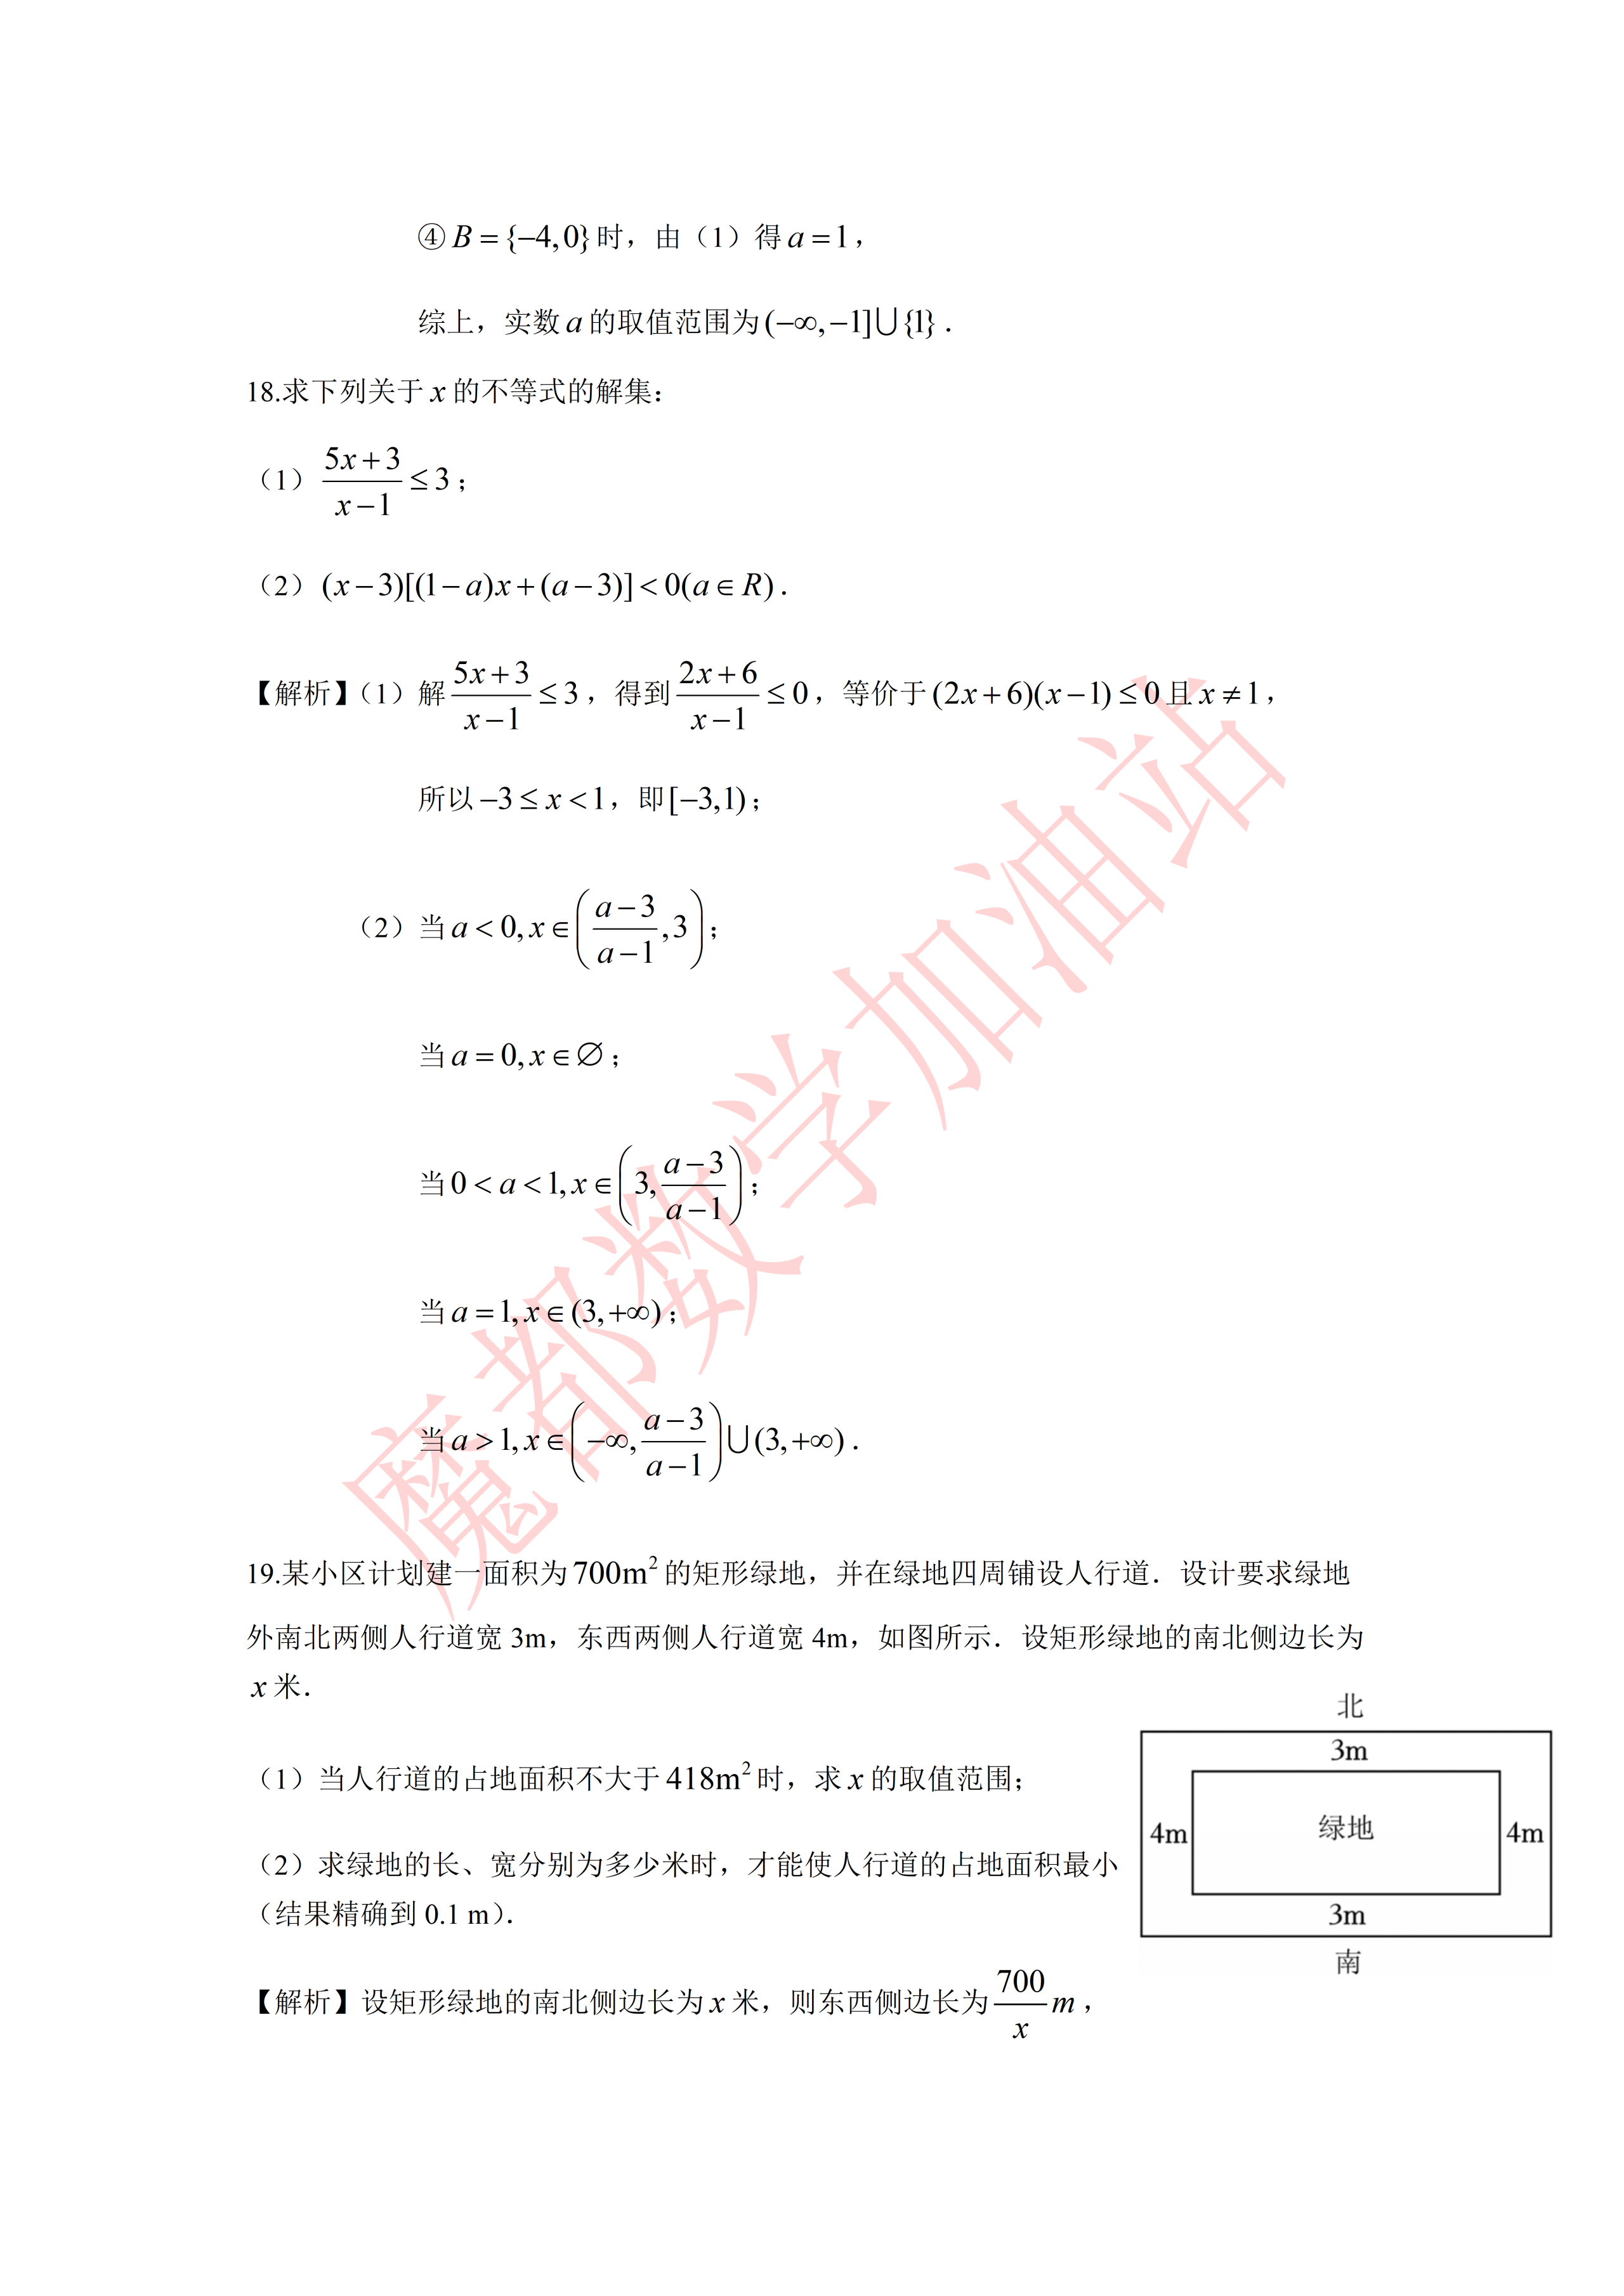
\includegraphics[width=.3\linewidth,trim=1791bp 484bp 107bp 2654bp,clip]{../原图/高一53_华师大二附中_10月月考/07.png}
\end{center}

\begin{enumerate}[label=(\arabic*)]
\item 当人行道的占地面积不大于 $418m^2$ 时，求 $x$ 的取值范围；
\item 求绿地的长、宽分别为多少米时，才能使人行道的占地面积最小（结果精确到 $0.1m$）.
\end{enumerate}

\ifanswer
\solbegin
\step{设矩形绿地的南北侧边长为 $x$ 米，则东西侧边长为 $\dfrac{700}{x}m$，}
\step{则人行道的占地面积为 $S=(x+8)\left(\dfrac{700}{x}+6\right)-700$，即 $S=6x+\dfrac{5600}{x}+48$.}
\stepm{(1)}{当人行道的占地面积不大于 $418m^2$ 时，$6x+\dfrac{5600}{x}+48\leqslant418$，}
\step{即 $6x^2-370x+5600\leqslant0$，解得 $\dfrac{80}{3}\leqslant x\leqslant35$，}
\step{故当人行道的占地面积不大于 $418m^2$ 时，$x\in\left[\dfrac{80}{3},35\right]$；}
\stepm{(2)}{$S=6x+\dfrac{5600}{x}+48\geqslant2\sqrt{6x\cdot\dfrac{5600}{x}}+48=80\sqrt{21}+48$，}
\step{当且仅当 $6x=\dfrac{5600}{x}$，即 $x=20\sqrt{\dfrac73}\approx30.6(m)$ 时，}
% 原卷如此，照录未改（80√21+48≈414.6，两处“414.4”疑笔误，见文件头“原卷笔误/存疑”第 6 条）
\step{$S$ 达到最小值 $80\sqrt{21}+48\approx414.4$，此时 $\dfrac{700}{x}\approx22.9(m)$，}
\step{所以当设计绿地的南北侧边长约为 $30.6m$，东西侧边长约为 $22.9m$ 时，}
\step{人行道的占地面积最小值为 $414.4(m^2)$.}
\solend
\fi

\ansspace[6]

\item 已知 $x\in\R$，符号 $[x]$ 表示不大于 $x$ 的最大整数，例如：$[2.3]=2$,$[2]=2$，$[-1.2]=-2$，令 $S(x)=[x]-[-x]$.

\begin{enumerate}[label=(\arabic*)]
\item 写出 $S(x)$ 为偶数（包括正、负偶数和 0）的充要条件，并证明；
\item 设方程 $|S(x)|=3$ 的解集为 $A$.

①集合 $B=\{x\mid x^2-ax-9\leqslant0,a\in\R\}$，若 $A\cap B=A$，求实数 $a$ 的取值范围；

②集合 $C=\{x\mid 2x^2-5kx+3k^2\geqslant0\}$，若 $A\cup C=\R$，求实数 $k$ 的取值范围.
\end{enumerate}

\ifanswer
\solbegin
\stepm{(1)}{$S(x)$ 为偶数的充要条件是 $x\in\Z$.}
\step{若 $x\in\Z$，则 $S(x)=[x]-[-x]=x-(-x)=2x$；}
\step{若 $x\notin\Z$，设 $[x]=n$，}
\step{则 $S(x)=[x]-[-x]=n-(-n-1)=2n+1=2[x]+1$；}
% 原卷如此，照录未改（“由①”按文意应为“由(1)”，见文件头“原卷笔误/存疑”第 3 条）
\stepm{(2)}{由①得 3 是奇数，$S(x)=\pm3$,$x\notin\Z$，}
\step{$S(x)=2[x]+1=\pm3$,$[x]=1$ 或 $-2$ 且 $x\notin\Z$，}
\step{所以 $A=(-2,-1)\cup(1,2)$；}
\stepm{①}{$A\cap B=A\Rightarrow A\subseteq B$，}
\step{设 $B=[x_1,x_2]$，其中 $x_1,x_2$ 是方程 $x^2-ax-9=0$ 的两实根，}
\step{设 $f(x)=x^2-ax-9$，}
\step{$[-2,2]\subseteq[x_1,x_2]\Leftrightarrow x_1\leqslant-2$,$x_2\geqslant2\Leftrightarrow\begin{cases}f(-2)\leqslant0\\ f(2)\leqslant0\end{cases}$}
\step{$\Leftrightarrow\begin{cases}(-2)^2-a\cdot(-2)-9\leqslant0, & a\leqslant\dfrac52\\ 2^2-2a-9\leqslant0, & a\geqslant-\dfrac52\end{cases}$，故 $a\in\left[-\dfrac52,\dfrac52\right]$；}
\step{注：若用求根公式 $\begin{cases}\dfrac{a+\sqrt{a^2+36}}{2}\geqslant2\Rightarrow a\geqslant-\dfrac52\\ \dfrac{a-\sqrt{a^2+36}}{2}\leqslant-2\Rightarrow a\leqslant\dfrac52\end{cases}$，结果正确，也得满分；}
\stepm{②}{$2x^2-5kx+3k^2=(x-k)(2x-3k)$.}
\step{$A\cup C=\R\Leftrightarrow\complement_\R A\subseteq C$.}
\step{记 $g(x)=2x^2-5kx+3k^2$，则 $\{x\mid g(x)<0\}\subseteq A$.}
\stepm{情况1：}{$k>0$ 时，$k<\dfrac32k$,$g(x)<0$ 的解集为 $\left(k,\dfrac32k\right)\subseteq(1,2)$，}
\step{故 $\begin{cases}k\geqslant1\\ \dfrac32k\leqslant2\end{cases}\Rightarrow1\leqslant k\leqslant\dfrac43$；}
\stepm{情况2：}{$k=0$ 时，$g(x)=2x^2\geqslant0$ 恒成立，$C=\R$,$A\cup C=\R$ 显然成立；}
\stepm{情况3：}{$k<0$ 时，$\dfrac32k<k$,$g(x)<0$ 的解集为 $\left(\dfrac32k,k\right)\subseteq(-2,-1)$，}
\step{故 $\begin{cases}\dfrac32k\geqslant-2\\ k\leqslant-1\end{cases}\Rightarrow-\dfrac43\leqslant k\leqslant-1$；}
\step{综上，$k\in\left[-\dfrac43,-1\right]\cup\{0\}\cup\left[1,\dfrac43\right]$.}
\solend
\fi

\ansspace[10]

\item 对于非空实数集 $M\subseteq(0,+\infty)$，若满足以下两个条件，则称 $M$ 为“极闭集”：

①$M$ 中至少含有 2 个元素，且 $1\notin M$；

②对于 $M$ 中任意两个不相等的元素 $x,y$，定义 $x*y=\dfrac{xy+1}{x+y}$，且 $x*y\in M$.

\begin{enumerate}[label=(\arabic*)]
\item 判断集合 $A=\left\{\dfrac12,2\right\}$ 与区间 $B=(1,+\infty)$ 是否为“极闭集”，并说明理由；
\item 若 $M$ 是“极闭集”，证明：集合 $M$ 中不可能所有元素都小于 1；
\item 证明：不存在任何有限的“极闭集”.
\end{enumerate}

\ifanswer
\solbegin
% 原卷如此，照录未改（首行集合按题干应为 {1/2,2}，见文件头“原卷笔误/存疑”第 7 条）
\stepm{(1)}{对于集合 $A=\left\{\dfrac12,1\right\}$，$\dfrac12*2=\dfrac45$，}
\step{因为 $\dfrac45\notin A$，不满足条件②，所以集合 $A$ 不是“极闭集”.}
\step{对于区间 $B$，满足条件①.}
\step{任取 $B$ 中两个不相等的元素 $x,y$，则 $x>1$,$y>1$.}
\step{$x*y-1=\dfrac{xy+1}{x+y}-1=\dfrac{(x-1)(y-1)}{x+y}>0$，所以 $x*y>1$，}
\step{这说明 $x*y\in B$ 恒成立，满足条件②，所以 $B$ 是“极闭集”.}
\stepm{(2)}{假设集合 $M$ 中所有元素都小于 1，}
\step{在 $M$ 中取 $0<x<y<1$,$x*y-1=\dfrac{xy+1}{x+y}-1=\dfrac{(x-1)(y-1)}{x+y}>0$，}
\step{所以 $x*y>1$，与“集合 $M$ 中所有元素都小于 1”矛盾，}
\step{假设不成立，集合 $M$ 中不可能所有元素都小于 1，得证.}
\stepm{(3)}{由②得，任何一个“极闭集”$M$ 中，必然至少存在一个大于 1 的元素，}
\stepm{情况1：}{若 $M$ 中至少存在两个大于 1 的元素，}
\step{设其中两个不相等的元素为 $x$ 和 $y_1$，且 $x>y_1>1$，}
\step{令 $y_{n+1}=x*y_n$,$n\geqslant1$,$y_{n+1}-1=x*y_n-1=\dfrac{(x-1)(y_n-1)}{xy_n+1}>0$，}
\step{如果 $y_n\geqslant1$，则显然 $y_{n+1}\geqslant1$，作差 $y_n-y_{n+1}=\dfrac{y_n^2-1}{x+y_n}>0$，}
\step{由此 $x>y_1>y_2>y_3>\cdots>1$，与有限集矛盾.}
\stepm{情况2：}{若 $M$ 中恰好只有一个元素大于 1，}
\step{设这个唯一大于 1 的元素为 $m$.}
\step{因为 $M$ 至少有两个元素，所以 $M$ 中必然至少存在一个元素 $a_1<1$，}
\step{令 $a_{n+1}=m*a_n$,$n\geqslant1$，}
\step{又 $a_{n+1}-1=m*a_n-1=\dfrac{(m-1)(a_n-1)}{m+a_n}<0$，故 $a_{n+1}<1$，}
\step{作差 $a_{n+1}-a_n=\dfrac{1-a_n^2}{m+a_n}>0$，由此 $a_1<a_2<a_3<\cdots<1$，与有限集矛盾.}
\step{因此，不存在任何有限的“极闭集”. 原命题得证.}
\solend
\fi

\ansspace*[10]

\end{enumerate}

\end{document}
"
% 紧凑版：xelatex "\def\iscompact{1}% 高一53_华师大二附中_10月月考.tex
%   —— 高一上数学“2026-2027 年华师大二附中高一上 10 月月考”（讲评版）
% 试卷版：xelatex 高一53_华师大二附中_10月月考.tex
% 答案版：xelatex "\def\isanswer{1}\input{高一53_华师大二附中_10月月考.tex}"
% 紧凑版：xelatex "\def\iscompact{1}\input{高一53_华师大二附中_10月月考.tex}"
%
% 原始材料：微信公众号“魔都数学加油站”文章，作者破晓，连载“27学年高一53”；
% 原文标题“27学年高一53——2026-2027年上海市华师大二附中高一上10月月考”；
% 原文链接：https://mp.weixin.qq.com/s/fpSnoF-gJEEWyxAoPC_bZA。
% 页面标注发布时间 2026-10-09 17:15（上海）。
% 正文为 11 张 PNG 页：第 01—06、08、10 页 4762×6735，第 07、09、11 页 2560×3620
% （**同一篇各页分辨率不同**），均按页序读取。11 页全为试卷正文页（卷首标题在第 1 页页顶，
% 卷末解答题第 21 题解析止于第 11 页），无封面页、目录页、二维码或宣传页。
% 粉色斜排“魔都数学加油站”为卷面水印，与公众号页脚一并未录入。
%
% 卷首标题：照卷面印作“2026--2027 年华师大二附中高一上 10 月月考”（公众号标题中的“上海市”
% 卷面标题行没有，本稿照卷面），年份区间按全稿惯例排 en dash。原卷只有一行标题、无副标题。
%
% 篇幅与题号：原卷自第 3 题起编号（第 1、2 题不在本卷内）。填空题 3—12（10 题）、
% 选择题 13—16（4 题）、解答题 17—21（5 题），共 19 题。本稿沿用原节与原题号，
% 只改排为全稿统一的大节样式（原卷小节标题为“一、填空题”“二、选择题”“三、解答题”）。
%
% 讲评版：原卷每题下直接印【答案】或【解析】。**第 13 题没有任何【答案】/【解析】段**，
% 答案“C”直接印在题干括号内（“一定不是(  C  )”），本稿按 高一37 第 13 题的成例把括号留空、
% 答案另提为 \ans{$C$}；其余 18 题都只印【解析】，按全稿口径这类题不另提 \ans{}——其中
% 选择题第 14、15、16 题的结论写在解析末句（“故选 B／D／C”），亦照录在解析内。
%
% 副标题：原卷未印副标题。本稿按“知识模块”口径标作“集合与常用逻辑用语、不等式”：
% 19 题中集合与常用逻辑用语 12 题（集合类 9 题——第 4、5、12、13、15、16、17、20、21 题；
% 逻辑类 3 题——第 3、9、14 题），不等式 7 题（含一元二次方程与绝对值方程：第 6、7、8、10、
% 11、18、19 题，其中第 11 题实为奇偶分析下的集合计数题，暂挂不等式），两类均超三分之一，
% 故并标。口径同 高一46、高一47、高一48、高一51、高一52。
%
% 与原卷的排版差异：
%   ① 原卷每题下直接印【解析】，本稿按全稿惯例将答案与解析置于答案版，试卷版保持干净；
%      第 13 题印在题干括号内的答案“C”同样移入 \ans{}，见上；
%   ② 原卷未印副标题，本稿按“知识模块”口径补出；
%   ③ 原卷填空横线约两个字宽，本稿按全稿惯例统一排 \blankline[4.4em]；
%      选择题的作答括号原卷排半角“(    )”，本稿按全稿惯例排 \mbox{（\quad）}；
%   ④ 原卷实数集排斜体/粗体 $R$、$\mathbf{R}$（第 4、6、7、18、20 题等处），本稿按全稿惯例
%      改用 $\R$；空集记号统一为 \varnothing；
%   ⑤ 原卷在数学式内多处用半角逗号（如 $x_1,x_2$、$|S|,|T|$、$a\neq0,c\neq0$），均照录未强改；
%      句末句点按全稿惯例排西文句点（原卷“故选 B．”一类全角句点亦从宽排作“.”）；
%   ⑥ 第 17—21 题的子问原卷各自另起一行，本稿按全稿惯例用 enumerate 的 (1)(2)(3)；
%      第 20 题 (2) 问下的①②两行是题干的一部分，照录为行首①②标号（不入 enumerate）；
%      解析中的子问标号一律用 \stepm{(1)}{…}，解析中的①②③④分情形用 \stepm{①}{…}；
%   ⑦ 第 12、20、21 题解析里的“情况1:”至“情况3:”标号原卷排**红色加粗**（全卷共 6 处），
%      全库无红色排字先例，本稿按全稿子题标号样式排 \stepm{情况1：}{…}（加粗着色、不改黑色基调），
%      冒号照原卷排全角；
%   ⑧ 第 19 题的示意图原卷排在题干右侧（与题干、(1) 问同高），本稿居中排在题干之后、
%      子问之前，并在 \item 前加 \needvspace 整块推走；图自原图第 07 页裁切（trim），不另存图片文件；
%   ⑨ 每道解答题原卷未留作答空白，本稿按全稿惯例加 \ansspace。
%
% 原卷笔误/存疑（均照录未改，正文对应处另有 % 注）：
%   1. 第 14 题解析末行“例如 $a=1$，$b=-1$，及必要性不成立”，“及”按文意应为“即”；
%   2. 第 15 题解析第 3 行 $\dfrac1{a+b\sqrt2}=\dfrac a{a^2-2b}+\left(-\dfrac b{a^2-2b}\right)\cdot\sqrt2$，
%      分母两处均作 $a^2-2b$，按通分应为 $a^2-2b^2$（结论 $C=X$ 不受影响）；
%   3. 第 20 题 (2) 问解析首行“由①得 3 是奇数”，按文意应为“由(1)得”（①是 (2) 问下自己
%      的子问标号，奇偶性结论出自 (1) 问）；
%   4. 第 11 题解析“只有奇数的有 $C_4^2+1=7$ 个”，按组合意义应为 $C_4^2+C_4^4=7$
%      （“$+1$”当指 4 个奇数全取的 1 种），数值无误；
%   5. 第 18 题 (2) 问解析“当 $a=0$,$x\in\varnothing$”，按文意应为“解集为 $\varnothing$”；
%   6. 第 19 题 (2) 问解析“$S$ 达到最小值 $80\sqrt{21}+48\approx414.4$”与末行
%      “人行道的占地面积最小值为 $414.4(m^2)$”，两处按 $80\sqrt{21}+48\approx414.6$，疑笔误；
%   7. 第 21 题 (1) 问解析首行“对于集合 $A=\left\{\frac12,1\right\}$”，按题干应为
%      $A=\left\{\frac12,2\right\}$（计算 $\frac12*2=\frac45$ 用的正是 $2$）；
%   8. 第 12 题解析“所以 $A=(-\infty,-4]\cup[2,+\infty)$”一行行末无标点，体例不一，照录。
%
% 插图：1 张，自原图裁切（无 \begin{tikzpicture} 重排）：
%   · 第 19 题绿地示意图（外矩形内套矩形“绿地”，上“北 3m”、下“南 3m”、左右各“4m”）
%     ——原图第 07 页，原卷排于题干右侧。
%     裁框：x 1797–2447、y 2660–3136（含“北”“南”标注，四周各留约 6px），
%     trim=1791bp 484bp 107bp 2654bp（左／下／右／上），页宽 2560、页高 3620。
%
\documentclass[a4paper,11pt]{article}
\usepackage{common}

\begin{document}

\examtitlest[3]{2026--2027 年华师大二附中高一上 10 月月考}{集合与常用逻辑用语、不等式}

\bigsec{一、填空题}

\begin{enumerate}
\setcounter{enumi}{2}

\item “$x=2$”是“$x^2-3x+2=0$”的\blankline[4.4em]条件.

（选择其中之一填空：充分非必要、必要非充分、充分、既非充分又非必要）

\ifanswer
\solbegin
\step{由 $x^2-3x+2=0$ 得 $x=1$ 或 $x=2$，}
\step{则“$x=2$”是“$x^2-3x+2=0$”的充分不必要条件.}
\solend
\fi

\item 已知 $R$ 是全集，集合 $A=\{y\mid y=-x^2+1,x\in\R\}$，集合 $B=\{x\mid x=3+|a|,a\in\R\}$，则 $\overline{A\cup B}=$\blankline[4.4em].

\ifanswer
\solbegin
\step{$A=\{y\mid y=-x^2+1,x\in\R\}=(-\infty,1]$，$B=\{x\mid x=3+|a|,a\in\R\}=[3,+\infty)$，}
\step{所以 $\overline{A\cup B}=(1,3)$.}
\solend
\fi

\item 已知 $a$ 为常数，集合 $A=\{x\mid x^2+x-6=0\}$，集合 $B=\{x\mid ax-2=0\}$，且 $B\subseteq A$，则 $a$ 的所有取值构成的集合为\blankline[4.4em].

\ifanswer
\solbegin
\step{集合 $A=\{-3,2\}$，因为 $B\subseteq A$，则 $B=\varnothing$，$\{-3\}$，$\{2\}$，$\{-3,2\}$，}
\step{当 $B=\varnothing$ 时，$a=0$，当 $B=\{-3\}$ 时，$a=-\dfrac23$，当 $B=\{2\}$ 时，$a=1$，}
\step{当 $B=\{-3,2\}$ 时，不成立，故 $a$ 的取值集合为 $\left\{0,-\dfrac23,1\right\}$.}
\solend
\fi

\item 设 $a\in\R$，若关于 $x$ 的不等式 $x^2-ax<0$ 的解集是区间 $(0,1)$ 的真子集，则 $a$ 的取值范围是\blankline[4.4em].

\ifanswer
\solbegin
\step{因为关于 $x$ 的不等式 $x^2-ax<0$ 的解集是区间 $(0,1)$ 的真子集，}
\step{当 $a=0$ 时，不等式的解集为 $\varnothing$，符合题意；}
\step{当 $a>0$ 时，不等式的解集为 $(0,a)$，则 $0<a<1$，}
\step{当 $a<0$ 时，不等式的解集为 $(a,0)$，不符合题意，}
\step{故 $a$ 的范围为 $[0,1)$.}
\solend
\fi

\item 设 $x\in\R$，则方程 $|2x+3|-|x-2|=|3x+1|$ 的解集为\blankline[4.4em].

\ifanswer
\solbegin
\step{当 $x\leqslant-\dfrac32$ 时，原式$\Leftrightarrow-2x-3+x-2=-3x-1\Leftrightarrow x=2$，不合题意；}
\step{当 $-\dfrac32<x\leqslant-\dfrac13$ 时，原式$\Leftrightarrow2x+3+x-2=-3x-1\Leftrightarrow x=-\dfrac13$；}
\step{当 $-\dfrac13<x\leqslant2$ 时，原式$\Leftrightarrow2x+3+x-2=3x+1\Leftrightarrow1=1$ 即恒成立；}
\step{当 $x>2$ 时，原式$\Leftrightarrow2x+3+2-x=3x+1\Leftrightarrow x=2$，不合题意；}
\step{故 $x\in\left[-\dfrac13,2\right]$.}
\solend
\fi

\item 已知关于 $x$ 的一元二次方程 $x^2+(4m+1)x+2m-1=0$．若方程的两根为 $x_1$、$x_2$，且满足 $\dfrac1{x_1}+\dfrac1{x_2}=-\dfrac12$，则实数 $m=$\blankline[4.4em].

\ifanswer
\solbegin
\step{由于判别式$\Delta=16m^2+5>0$恒成立，}
\step{不论 $m$ 为任何实数，方程总有两个不相等的实数根.}
\step{$\dfrac1{x_1}+\dfrac1{x_2}=-\dfrac12$，即 $\dfrac{x_1+x_2}{x_1x_2}=-\dfrac12$，由根与系数的关系得 $\dfrac{-4m-1}{2m-1}=-\dfrac12$，}
\step{解得 $m=-\dfrac12$.}
\solend
\fi

\item 已知 $\dfrac1{x-2}\geqslant1$ 是 $|x-a|<2$ 的充分非必要条件，则实数 $a$ 的取值范围是\blankline[4.4em].

\ifanswer
\solbegin
\step{由 $\dfrac1{x-2}\geqslant1$ 得 $\dfrac{3-x}{x-2}\geqslant0$，解得 $2<x\leqslant3$，由 $|x-a|<2$ 得 $a-2<x<a+2$，}
\step{因为 $\dfrac1{x-2}\geqslant1$ 是 $|x-a|<2$ 的充分非必要条件，}
\step{所以 $\{x\mid 2<x\leqslant3\}\subset\{x\mid a-2<x<a+2\}$，所以 $\begin{cases}a-2\leqslant2\\ a+2>3\end{cases}$，解得 $1<a\leqslant4$，}
\step{即实数 $a$ 的取值范围是 $(1,4]$.}
\solend
\fi

\item 设 $x,y\in(0,+\infty)$，且 $x+4y=1$，则 $\dfrac1x+\dfrac1y$ 的最小值为\blankline[4.4em].

\ifanswer
\solbegin
\step{因为 $\dfrac1x+\dfrac1y=(x+4y)\left(\dfrac1x+\dfrac1y\right)=5+\dfrac{4y}{x}+\dfrac{x}{y}\geqslant5+2\sqrt{\dfrac{4y}{x}\cdot\dfrac{x}{y}}=9$，}
\step{当且仅当 $\dfrac{4y}{x}=\dfrac{x}{y}$，即 $x=2y$，即 $x=\dfrac13$,$y=\dfrac16$ 时取等号，故最小值为 $9$.}
\solend
\fi

\item 设非空集合 $Q\subseteq M$，当 $Q$ 中所有元素和为偶数时（集合为单元素时和为元素本身），称 $Q$ 是 $M$ 的偶子集. 若集合 $M=\{1,2,3,4,5,6,7\}$，则其偶子集 $Q$ 的个数为\blankline[4.4em].

\ifanswer
\solbegin
\step{偶子集可以分为只有奇数、偶数及偶数个奇数和偶数的集合，}
\step{奇数有 4 个，偶数有 3 个，}
% 原卷如此，照录未改：按组合意义应为 C_4^2+C_4^4=7（“+1”当指 4 个奇数全取的 1 种），
% 见文件头“原卷笔误/存疑”第 4 条
\step{只有奇数的有 $C_4^2+1=7$ 个，只有偶数的有 $C_3^1+C_3^2+1=7$ 个，}
\step{偶数个奇数和偶数的：两奇一偶 $C_4^2\cdot C_3^1=18$ 个，两奇二偶 $C_4^2\cdot C_3^2=18$ 个，}
\step{两奇三偶 $C_4^2\cdot C_3^3=6$ 个，四奇一偶 $C_4^4\cdot C_3^1=3$ 个，四奇二偶 $C_4^4\cdot C_3^2=3$ 个，}
\step{四奇三偶 $C_4^4\cdot C_3^3=1$ 个，所以共有 $7+7+18+18+6+3+3+1=63$ 个.}
\solend
\fi

\item 已知集合 $A=\{x\mid x^2+2x-8\geqslant0\}$,$B=\{x\mid x^2-2ax+2a\leqslant0\}$，且 $A\cap B$ 中恰有 3 个整数元素，则实数 $a$ 的取值范围为\blankline[4.4em].

\ifanswer
\solbegin
% 原卷如此，照录未改：此行行末无标点，见文件头“原卷笔误/存疑”第 8 条
\step{由 $x^2+2x-8\geqslant0$，得 $x\geqslant2$ 或 $x\leqslant-4$，所以 $A=(-\infty,-4]\cup[2,+\infty)$}
\step{对集合 $B$：$x^2-2ax+2a\leqslant0$,$\Delta=4a^2-8a=4a(a-2)\geqslant0$，}
\step{得 $a\leqslant0$ 或 $a\geqslant2$.}
\step{设方程 $x^2-2ax+2a=0$ 的两根为 $r_1,r_2$，}
\step{则 $B=[r_1,r_2]$,$r_1=a-\sqrt{a^2-2a}$,$r_2=a+\sqrt{a^2-2a}$，}
\stepm{情况1：}{$a\leqslant0$，}
\step{$r_2=a+\sqrt{a^2-2a}<a+\sqrt{a^2-2a+1}=a+|a-1|=a+1-a=1<2$，}
\step{$B$ 只在 $A$ 的左侧部分有交集，要使 $A\cap B$ 恰有 3 个整数元素，}
\step{这 3 个整数为 $-6,-5,-4$，于是 $r_1\in(-7,-6]$，}
\step{令 $f(x)=x^2-2ax+2a$，则 $\begin{cases}f(-7)=49+14a+2a>0\\ f(-6)=36+12a+2a\leqslant0\end{cases}\Rightarrow a\in\left(-\dfrac{49}{16},-\dfrac{18}{7}\right]$；}
\stepm{情况2：}{$a\geqslant2$，}
\step{$r_2=a+\sqrt{a^2-2a}\geqslant2$，}
\step{$r_1=a-\sqrt{a^2-2a}>a-\sqrt{a^2-2a+1}=a-|a-1|=a-(a-1)=1>-4$，}
\step{所以 $A\cap B=[2,r_2]$.}
\step{同理 $\begin{cases}f(4)=16-8a+2a\leqslant0\\ f(5)=25-10a+2a>0\end{cases}\Rightarrow a\in\left[\dfrac{8}{3},\dfrac{25}{8}\right)$；}
\step{综上，$a\in\left(-\dfrac{49}{16},-\dfrac{18}{7}\right]\cup\left[\dfrac{8}{3},\dfrac{25}{8}\right)$.}
\solend
\fi

\end{enumerate}

\bigsec{二、选择题}

\begin{enumerate}
\setcounter{enumi}{12}

% 第 13 题原卷无【答案】/【解析】段，答案“C”直接印在题干括号内，
% 按高一37 第 13 题的成例括号留空、答案另提为 \ans{}（见文件头）
\item 集合 $A=\{a,b,c\}$ 中的三个元素分别表示某一个三角形的三边长度，那么这个三角形一定不是\mbox{（\quad）}

\keepwithprev
A. 锐角三角形\qquad B. 钝角三角形

C. 等腰三角形\qquad D. 直角三角形

\ifanswer
\ans{$C$}
\fi

\item 设 $a$、$b$ 为实数，则“$a<b<0$”是“$\dfrac1a>\dfrac1b$”的\mbox{（\quad）}条件.

\keepwithprev
A. 充要\qquad B. 充分不必要

C. 必要不充分\qquad D. 既不充分也不必要

\ifanswer
\solbegin
\step{若 $a<b<0$，则 $\dfrac1a>\dfrac1b$ 一定成立，即充分性成立；}
% 原卷如此，照录未改（“及”按文意应为“即”，见文件头“原卷笔误/存疑”第 1 条）
\step{若 $\dfrac1a>\dfrac1b$ 成立，$a<b<0$ 不一定成立，例如 $a=1$，$b=-1$，及必要性不成立.}
\step{故选 $B$.}
\solend
\fi

\item 设 $Q$ 表示有理数集，集合 $X=\{x\mid x=a+b\sqrt2,a,b\in Q,x\neq0\}$，在下列集合中：①$\{2x\mid x\in X\}$②$\left\{\dfrac{x}{\sqrt2}\mid x\in X\right\}$③$\left\{\dfrac1x\mid x\in X\right\}$④$\{x^2\mid x\in X\}$，与 $X$ 相同的集合有\mbox{（\quad）}

\keepwithprev
A. ①②③④\qquad B. ②③④\qquad C. ①②④\qquad D. ①②③

\ifanswer
\solbegin
\step{$A=\{2x\mid x\in X\}$，$2(a+b\sqrt2)=p+q\sqrt2$ 得 $p=2a$，$q=2b$，$a=\dfrac p2$，$b=\dfrac q2$，}
\step{也是一一对应，$A=X$}
% 原卷如此，照录未改：分母两处均作 a^2-2b，按通分应为 a^2-2b^2，
% 见文件头“原卷笔误/存疑”第 2 条
\step{集合 $B=\left\{\dfrac{x}{\sqrt2}\mid x\in X\right\}$，$\dfrac{a+b\sqrt2}{\sqrt2}=b+\dfrac a2\cdot\sqrt2$，也是一一对应，$B=X$}
\step{集合 $C=\left\{\dfrac1x\mid x\in X\right\}$，$\dfrac{1}{a+b\sqrt2}=\dfrac{a}{a^2-2b}+\left(-\dfrac{b}{a^2-2b}\right)\cdot\sqrt2$，一一对应，$C=X$}
\step{集合 $D=\{x^2\mid x\in X\}$，$(a+b\sqrt2)^2=a^2+2b^2+2ab\sqrt2$，这个不能一一对应了，}
\step{集合 $D$ 包含于 $X$ 中.}
\step{故 $X$ 相同的集合有①②③，故选 $D$.}
\solend
\fi

\item 集合 $S=\{x\mid(x+a)(x^2+bx+c)=0\}$,$T=\{x\mid(ax+1)(cx^2+bx+1)=0\}$，其中 $a,b,c$ 为实数，若 $|S|,|T|$ 分别表示集合 $S,T$ 的元素个数，则 $|S|-|T|$ 的所有可能取值集合为\mbox{（\quad）}

\keepwithprev
A. $\{0\}$\qquad B. $\{1\}$\qquad C. $\{0,1\}$\qquad D. $\{-1,0,1\}$

\ifanswer
\solbegin
\stepm{①}{$a\neq0,c\neq0$ 时.}
\step{$S$ 中 $x+a=0$ 的根 $x=-a$;$T$ 中 $ax+1=0$ 的根 $x=-\dfrac1a$.}
\step{$S$ 中的 $x^2+bx+c=0$ 若无实根，则 $T$ 中的 $cx^2+bx+1=0$ 也无实根；}
\step{又设 $S$ 的 $x^2+bx+c=0$ 的根为 $r(r\neq0)$，则 $T$ 的 $cx^2+bx+1=0$ 的根为 $\dfrac1r$.}
\step{（因为 $r^2+br+c=0\Rightarrow c\cdot\left(\dfrac1r\right)^2+b\cdot\dfrac1r+1=0$）}
\step{即 $a\neq0,c\neq0$ 时，}
\step{$S$ 与 $T$ 的实根存在一一对应关系 $x\leftrightarrow\dfrac1x$,$|S|=|T|,$$|S|-|T|=0$；}
\stepm{②}{$a=0,c\neq0$ 时.}
\step{$S$ 中多出一个根 $x=0$，而 $T$ 中无此根，$|S|=|T|+1$，即 $|S|-|T|=1$；}
\stepm{③}{$a\neq0,c=0$ 时.}
\step{则 $S$ 中仍有根 $x=0$，而 $T$ 中无 0 根，同样 $|S|-|T|=1$.}
\stepm{④}{$a=0,c=0$ 时.}
\step{同样 $S$ 含有根 0，而 $T$ 中不含 0，仍有 $|S|-|T|=1$.}
\step{综上，$|S|-|T|$ 所有可能取值为 0 和 1，故选 $C$.}
\solend
\fi

\end{enumerate}

\bigsec{三、解答题}

\begin{enumerate}
\setcounter{enumi}{16}

\item 已知集合 $A=\{x\mid x^2+4x=0\}$，$B=\{x\mid x^2+2(a+1)x+a^2-1=0\}$.

\begin{enumerate}[label=(\arabic*)]
\item 若 $A$ 是 $B$ 的子集，求实数 $a$ 的值；
\item 若 $B$ 是 $A$ 的子集，求实数 $a$ 的取值范围.
\end{enumerate}

\ifanswer
\solbegin
\stepm{(1)}{因为 $A=\{-4,0\}$，$B=\{x\mid x^2+2(a+1)x+a^2-1=0\}$，又 $A\subseteq B$，}
\step{所以 $A=B$，所以 $\begin{cases}-4+0=-2(a+1)\\ -4\times0=a^2-1\end{cases}$，所以 $a=1$；}
\stepm{(2)}{因为 $B$ 是 $A$ 的子集，所以 $B=\varnothing$ 或 $B=\{-4\}$ 或 $B=\{0\}$ 或 $B=\{-4,0\}$，}
\stepm{①}{$B=\varnothing$ 时，$\Delta=4(a+1)^2-4(a^2-1)<0$，所以 $a<-1$；}
\stepm{②}{$B=\{-4\}$ 时，$\begin{cases}-4+(-4)=-2(a+1)\\ -4\times(-4)=a^2-1\end{cases}$，无解；}
\stepm{③}{$B=\{0\}$ 时，$\begin{cases}0+0=-2(a+1)\\ 0\times0=a^2-1\end{cases}$，所以 $a=-1$；}
\stepm{④}{$B=\{-4,0\}$ 时，由（1）得 $a=1$，}
\step{综上，实数 $a$ 的取值范围为 $(-\infty,-1]\cup\{1\}$.}
\solend
\fi

\ansspace[6]

\item 求下列关于 $x$ 的不等式的解集：

\begin{enumerate}[label=(\arabic*)]
\item $\dfrac{5x+3}{x-1}\leqslant3$；
\item $(x-3)[(1-a)x+(a-3)]<0$ ($a\in\R$).
\end{enumerate}

\ifanswer
\solbegin
\stepm{(1)}{解 $\dfrac{5x+3}{x-1}\leqslant3$，得到 $\dfrac{2x+6}{x-1}\leqslant0$，等价于 $(2x+6)(x-1)\leqslant0$ 且 $x\neq1$，}
\step{所以 $-3\leqslant x<1$，即 $[-3,1)$；}
\stepm{(2)}{当 $a<0$,$x\in\left(\dfrac{a-3}{a-1},3\right)$；}
% 原卷如此，照录未改（“x∈∅”按文意应为“解集为 ∅”，见文件头“原卷笔误/存疑”第 5 条）
\step{当 $a=0$,$x\in\varnothing$；}
\step{当 $0<a<1$,$x\in\left(3,\dfrac{a-3}{a-1}\right)$；}
\step{当 $a=1$,$x\in(3,+\infty)$；}
\step{当 $a>1$,$x\in\left(-\infty,\dfrac{a-3}{a-1}\right)\cup(3,+\infty)$.}
\solend
\fi

\ansspace[6]

\needvspace{13\baselineskip}

\item 某小区计划建一面积为 $700m^2$ 的矩形绿地，并在绿地四周铺设人行道. 设计要求绿地外南北两侧人行道宽 $3m$，东西两侧人行道宽 $4m$，如图所示. 设矩形绿地的南北侧边长为 $x$ 米.

\begin{center}
% 原图第 7 页题干绿地示意图直接裁取（原卷排于题干右侧）。
% 裁框取图形外框 x 1797–2447、y 2660–3136（含“北”“南”标注，四周各留约 6px），
% trim=左 1791bp／下 484bp／右 107bp／上 2654bp（页宽 2560、页高 3620）。
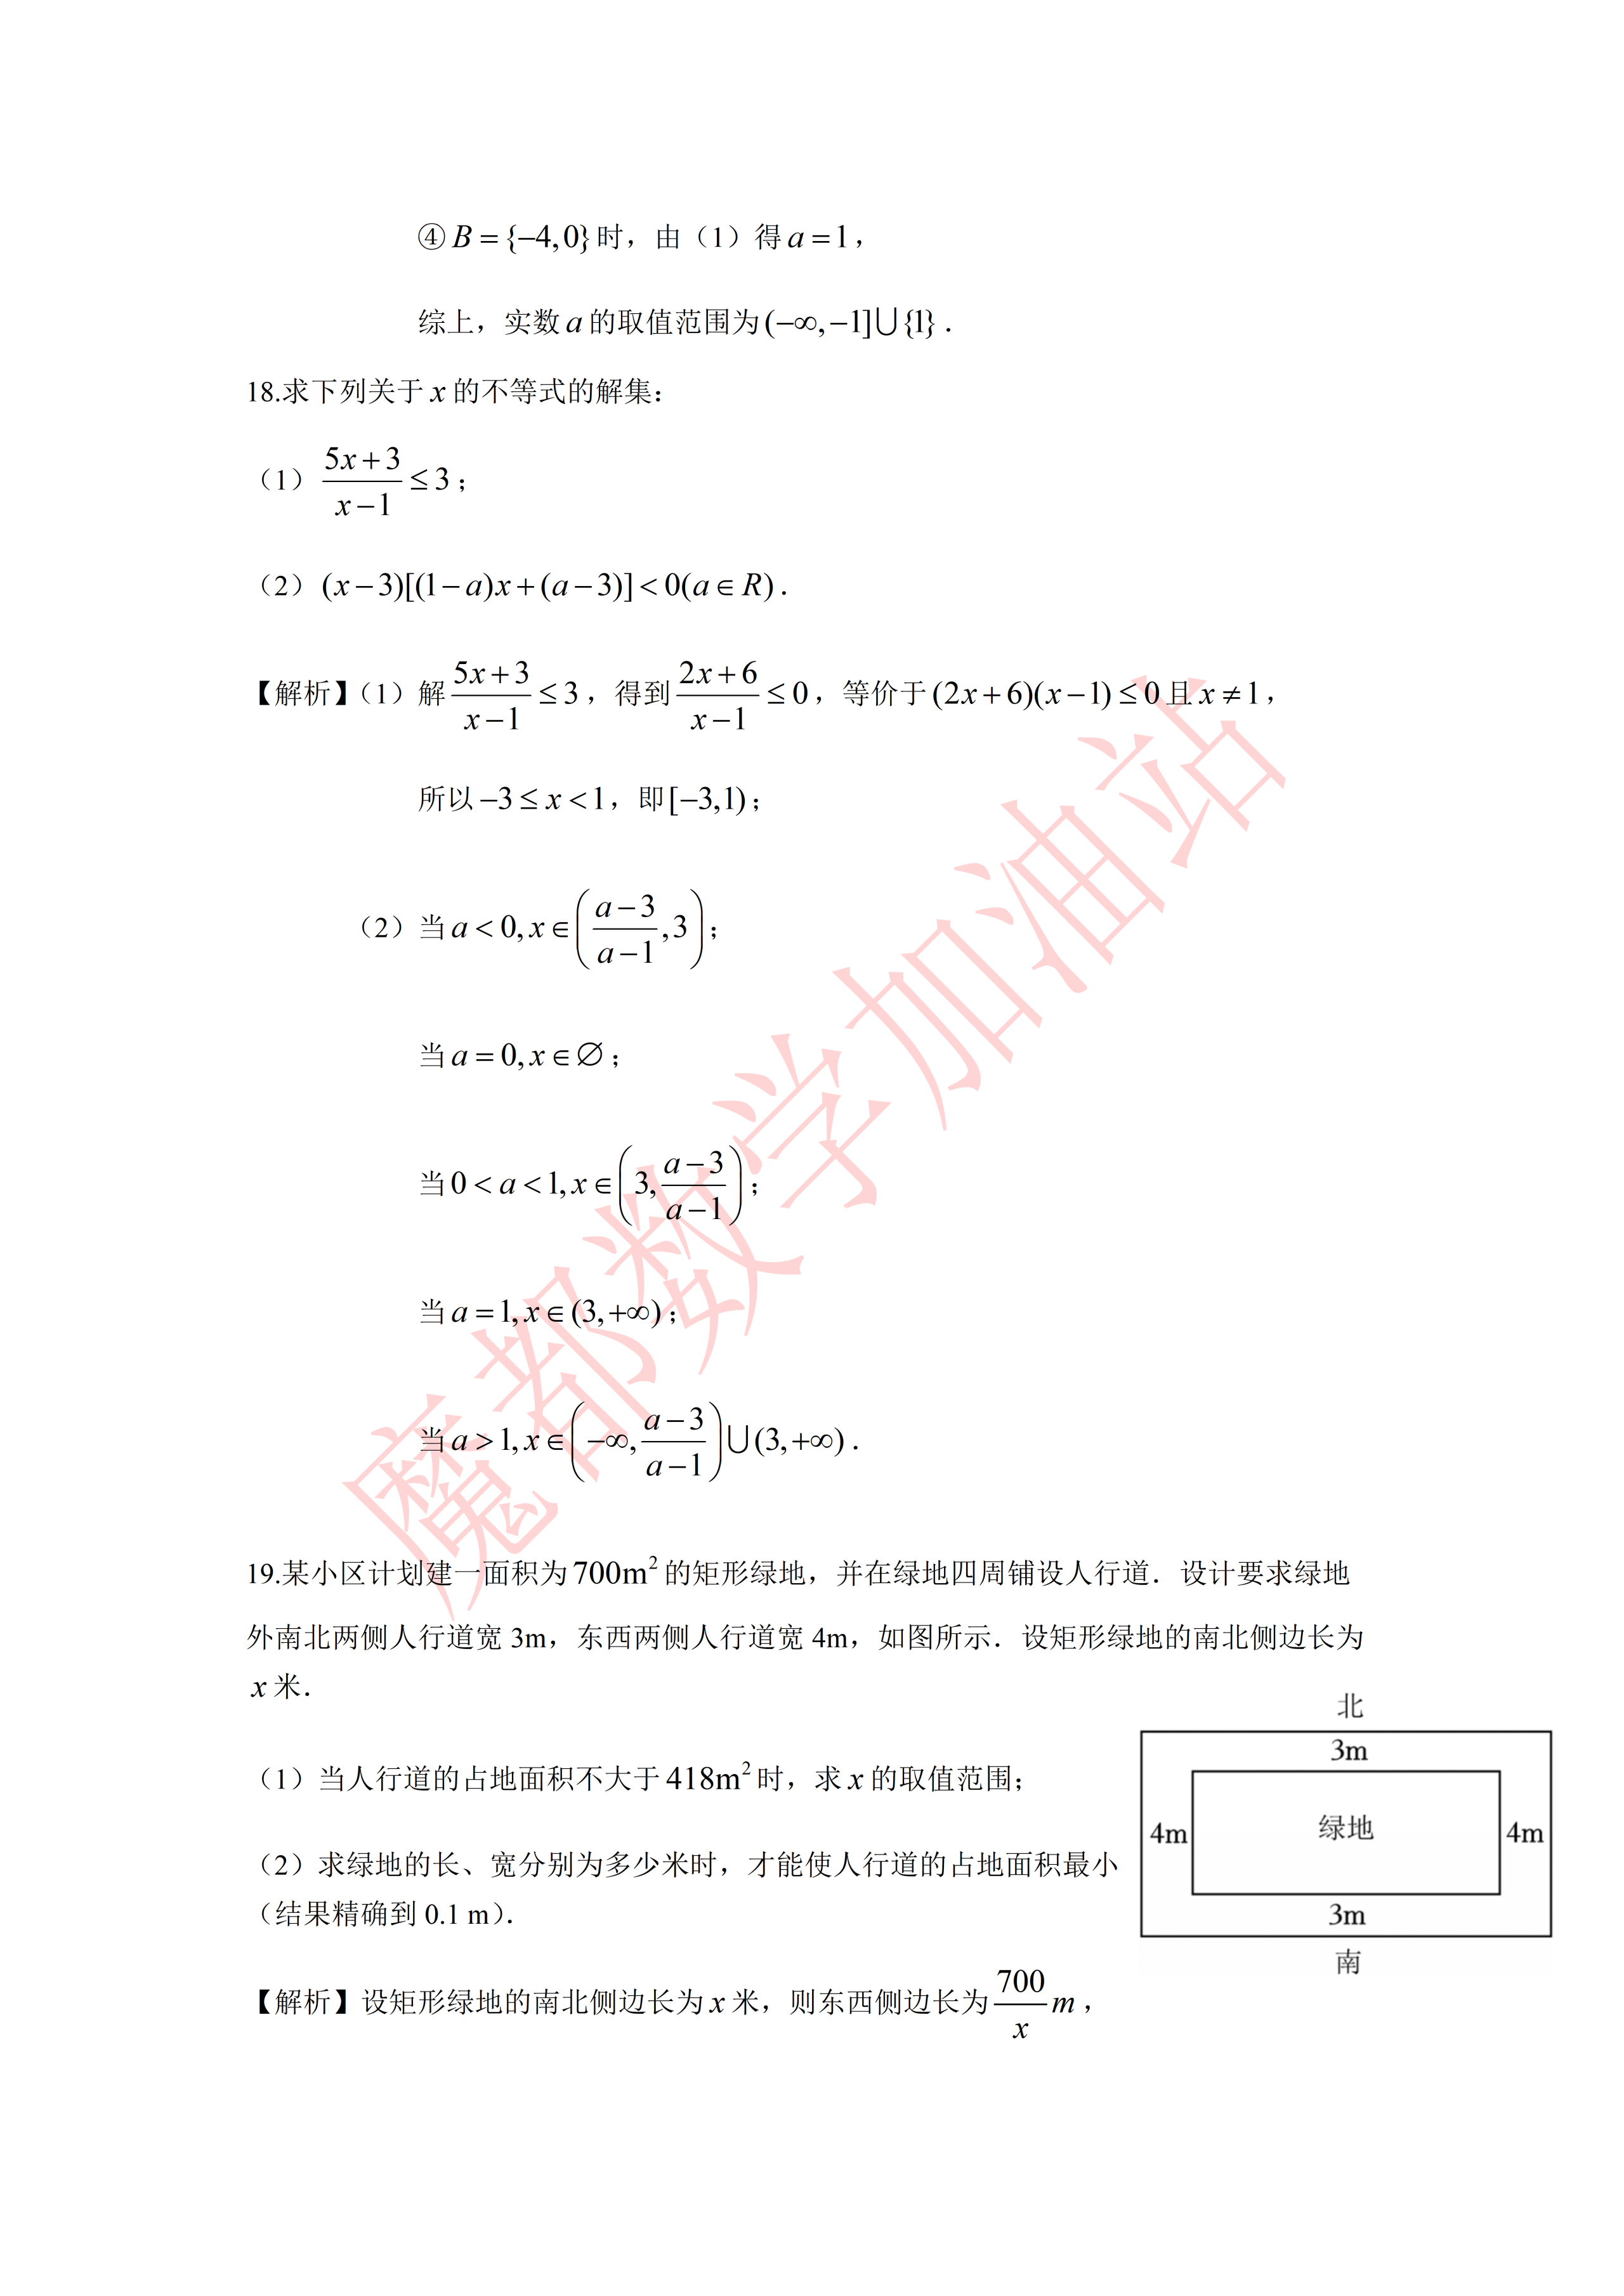
\includegraphics[width=.3\linewidth,trim=1791bp 484bp 107bp 2654bp,clip]{../原图/高一53_华师大二附中_10月月考/07.png}
\end{center}

\begin{enumerate}[label=(\arabic*)]
\item 当人行道的占地面积不大于 $418m^2$ 时，求 $x$ 的取值范围；
\item 求绿地的长、宽分别为多少米时，才能使人行道的占地面积最小（结果精确到 $0.1m$）.
\end{enumerate}

\ifanswer
\solbegin
\step{设矩形绿地的南北侧边长为 $x$ 米，则东西侧边长为 $\dfrac{700}{x}m$，}
\step{则人行道的占地面积为 $S=(x+8)\left(\dfrac{700}{x}+6\right)-700$，即 $S=6x+\dfrac{5600}{x}+48$.}
\stepm{(1)}{当人行道的占地面积不大于 $418m^2$ 时，$6x+\dfrac{5600}{x}+48\leqslant418$，}
\step{即 $6x^2-370x+5600\leqslant0$，解得 $\dfrac{80}{3}\leqslant x\leqslant35$，}
\step{故当人行道的占地面积不大于 $418m^2$ 时，$x\in\left[\dfrac{80}{3},35\right]$；}
\stepm{(2)}{$S=6x+\dfrac{5600}{x}+48\geqslant2\sqrt{6x\cdot\dfrac{5600}{x}}+48=80\sqrt{21}+48$，}
\step{当且仅当 $6x=\dfrac{5600}{x}$，即 $x=20\sqrt{\dfrac73}\approx30.6(m)$ 时，}
% 原卷如此，照录未改（80√21+48≈414.6，两处“414.4”疑笔误，见文件头“原卷笔误/存疑”第 6 条）
\step{$S$ 达到最小值 $80\sqrt{21}+48\approx414.4$，此时 $\dfrac{700}{x}\approx22.9(m)$，}
\step{所以当设计绿地的南北侧边长约为 $30.6m$，东西侧边长约为 $22.9m$ 时，}
\step{人行道的占地面积最小值为 $414.4(m^2)$.}
\solend
\fi

\ansspace[6]

\item 已知 $x\in\R$，符号 $[x]$ 表示不大于 $x$ 的最大整数，例如：$[2.3]=2$,$[2]=2$，$[-1.2]=-2$，令 $S(x)=[x]-[-x]$.

\begin{enumerate}[label=(\arabic*)]
\item 写出 $S(x)$ 为偶数（包括正、负偶数和 0）的充要条件，并证明；
\item 设方程 $|S(x)|=3$ 的解集为 $A$.

①集合 $B=\{x\mid x^2-ax-9\leqslant0,a\in\R\}$，若 $A\cap B=A$，求实数 $a$ 的取值范围；

②集合 $C=\{x\mid 2x^2-5kx+3k^2\geqslant0\}$，若 $A\cup C=\R$，求实数 $k$ 的取值范围.
\end{enumerate}

\ifanswer
\solbegin
\stepm{(1)}{$S(x)$ 为偶数的充要条件是 $x\in\Z$.}
\step{若 $x\in\Z$，则 $S(x)=[x]-[-x]=x-(-x)=2x$；}
\step{若 $x\notin\Z$，设 $[x]=n$，}
\step{则 $S(x)=[x]-[-x]=n-(-n-1)=2n+1=2[x]+1$；}
% 原卷如此，照录未改（“由①”按文意应为“由(1)”，见文件头“原卷笔误/存疑”第 3 条）
\stepm{(2)}{由①得 3 是奇数，$S(x)=\pm3$,$x\notin\Z$，}
\step{$S(x)=2[x]+1=\pm3$,$[x]=1$ 或 $-2$ 且 $x\notin\Z$，}
\step{所以 $A=(-2,-1)\cup(1,2)$；}
\stepm{①}{$A\cap B=A\Rightarrow A\subseteq B$，}
\step{设 $B=[x_1,x_2]$，其中 $x_1,x_2$ 是方程 $x^2-ax-9=0$ 的两实根，}
\step{设 $f(x)=x^2-ax-9$，}
\step{$[-2,2]\subseteq[x_1,x_2]\Leftrightarrow x_1\leqslant-2$,$x_2\geqslant2\Leftrightarrow\begin{cases}f(-2)\leqslant0\\ f(2)\leqslant0\end{cases}$}
\step{$\Leftrightarrow\begin{cases}(-2)^2-a\cdot(-2)-9\leqslant0, & a\leqslant\dfrac52\\ 2^2-2a-9\leqslant0, & a\geqslant-\dfrac52\end{cases}$，故 $a\in\left[-\dfrac52,\dfrac52\right]$；}
\step{注：若用求根公式 $\begin{cases}\dfrac{a+\sqrt{a^2+36}}{2}\geqslant2\Rightarrow a\geqslant-\dfrac52\\ \dfrac{a-\sqrt{a^2+36}}{2}\leqslant-2\Rightarrow a\leqslant\dfrac52\end{cases}$，结果正确，也得满分；}
\stepm{②}{$2x^2-5kx+3k^2=(x-k)(2x-3k)$.}
\step{$A\cup C=\R\Leftrightarrow\complement_\R A\subseteq C$.}
\step{记 $g(x)=2x^2-5kx+3k^2$，则 $\{x\mid g(x)<0\}\subseteq A$.}
\stepm{情况1：}{$k>0$ 时，$k<\dfrac32k$,$g(x)<0$ 的解集为 $\left(k,\dfrac32k\right)\subseteq(1,2)$，}
\step{故 $\begin{cases}k\geqslant1\\ \dfrac32k\leqslant2\end{cases}\Rightarrow1\leqslant k\leqslant\dfrac43$；}
\stepm{情况2：}{$k=0$ 时，$g(x)=2x^2\geqslant0$ 恒成立，$C=\R$,$A\cup C=\R$ 显然成立；}
\stepm{情况3：}{$k<0$ 时，$\dfrac32k<k$,$g(x)<0$ 的解集为 $\left(\dfrac32k,k\right)\subseteq(-2,-1)$，}
\step{故 $\begin{cases}\dfrac32k\geqslant-2\\ k\leqslant-1\end{cases}\Rightarrow-\dfrac43\leqslant k\leqslant-1$；}
\step{综上，$k\in\left[-\dfrac43,-1\right]\cup\{0\}\cup\left[1,\dfrac43\right]$.}
\solend
\fi

\ansspace[10]

\item 对于非空实数集 $M\subseteq(0,+\infty)$，若满足以下两个条件，则称 $M$ 为“极闭集”：

①$M$ 中至少含有 2 个元素，且 $1\notin M$；

②对于 $M$ 中任意两个不相等的元素 $x,y$，定义 $x*y=\dfrac{xy+1}{x+y}$，且 $x*y\in M$.

\begin{enumerate}[label=(\arabic*)]
\item 判断集合 $A=\left\{\dfrac12,2\right\}$ 与区间 $B=(1,+\infty)$ 是否为“极闭集”，并说明理由；
\item 若 $M$ 是“极闭集”，证明：集合 $M$ 中不可能所有元素都小于 1；
\item 证明：不存在任何有限的“极闭集”.
\end{enumerate}

\ifanswer
\solbegin
% 原卷如此，照录未改（首行集合按题干应为 {1/2,2}，见文件头“原卷笔误/存疑”第 7 条）
\stepm{(1)}{对于集合 $A=\left\{\dfrac12,1\right\}$，$\dfrac12*2=\dfrac45$，}
\step{因为 $\dfrac45\notin A$，不满足条件②，所以集合 $A$ 不是“极闭集”.}
\step{对于区间 $B$，满足条件①.}
\step{任取 $B$ 中两个不相等的元素 $x,y$，则 $x>1$,$y>1$.}
\step{$x*y-1=\dfrac{xy+1}{x+y}-1=\dfrac{(x-1)(y-1)}{x+y}>0$，所以 $x*y>1$，}
\step{这说明 $x*y\in B$ 恒成立，满足条件②，所以 $B$ 是“极闭集”.}
\stepm{(2)}{假设集合 $M$ 中所有元素都小于 1，}
\step{在 $M$ 中取 $0<x<y<1$,$x*y-1=\dfrac{xy+1}{x+y}-1=\dfrac{(x-1)(y-1)}{x+y}>0$，}
\step{所以 $x*y>1$，与“集合 $M$ 中所有元素都小于 1”矛盾，}
\step{假设不成立，集合 $M$ 中不可能所有元素都小于 1，得证.}
\stepm{(3)}{由②得，任何一个“极闭集”$M$ 中，必然至少存在一个大于 1 的元素，}
\stepm{情况1：}{若 $M$ 中至少存在两个大于 1 的元素，}
\step{设其中两个不相等的元素为 $x$ 和 $y_1$，且 $x>y_1>1$，}
\step{令 $y_{n+1}=x*y_n$,$n\geqslant1$,$y_{n+1}-1=x*y_n-1=\dfrac{(x-1)(y_n-1)}{xy_n+1}>0$，}
\step{如果 $y_n\geqslant1$，则显然 $y_{n+1}\geqslant1$，作差 $y_n-y_{n+1}=\dfrac{y_n^2-1}{x+y_n}>0$，}
\step{由此 $x>y_1>y_2>y_3>\cdots>1$，与有限集矛盾.}
\stepm{情况2：}{若 $M$ 中恰好只有一个元素大于 1，}
\step{设这个唯一大于 1 的元素为 $m$.}
\step{因为 $M$ 至少有两个元素，所以 $M$ 中必然至少存在一个元素 $a_1<1$，}
\step{令 $a_{n+1}=m*a_n$,$n\geqslant1$，}
\step{又 $a_{n+1}-1=m*a_n-1=\dfrac{(m-1)(a_n-1)}{m+a_n}<0$，故 $a_{n+1}<1$，}
\step{作差 $a_{n+1}-a_n=\dfrac{1-a_n^2}{m+a_n}>0$，由此 $a_1<a_2<a_3<\cdots<1$，与有限集矛盾.}
\step{因此，不存在任何有限的“极闭集”. 原命题得证.}
\solend
\fi

\ansspace*[10]

\end{enumerate}

\end{document}
"
%
% 原始材料：微信公众号“魔都数学加油站”文章，作者破晓，连载“27学年高一53”；
% 原文标题“27学年高一53——2026-2027年上海市华师大二附中高一上10月月考”；
% 原文链接：https://mp.weixin.qq.com/s/fpSnoF-gJEEWyxAoPC_bZA。
% 页面标注发布时间 2026-10-09 17:15（上海）。
% 正文为 11 张 PNG 页：第 01—06、08、10 页 4762×6735，第 07、09、11 页 2560×3620
% （**同一篇各页分辨率不同**），均按页序读取。11 页全为试卷正文页（卷首标题在第 1 页页顶，
% 卷末解答题第 21 题解析止于第 11 页），无封面页、目录页、二维码或宣传页。
% 粉色斜排“魔都数学加油站”为卷面水印，与公众号页脚一并未录入。
%
% 卷首标题：照卷面印作“2026--2027 年华师大二附中高一上 10 月月考”（公众号标题中的“上海市”
% 卷面标题行没有，本稿照卷面），年份区间按全稿惯例排 en dash。原卷只有一行标题、无副标题。
%
% 篇幅与题号：原卷自第 3 题起编号（第 1、2 题不在本卷内）。填空题 3—12（10 题）、
% 选择题 13—16（4 题）、解答题 17—21（5 题），共 19 题。本稿沿用原节与原题号，
% 只改排为全稿统一的大节样式（原卷小节标题为“一、填空题”“二、选择题”“三、解答题”）。
%
% 讲评版：原卷每题下直接印【答案】或【解析】。**第 13 题没有任何【答案】/【解析】段**，
% 答案“C”直接印在题干括号内（“一定不是(  C  )”），本稿按 高一37 第 13 题的成例把括号留空、
% 答案另提为 \ans{$C$}；其余 18 题都只印【解析】，按全稿口径这类题不另提 \ans{}——其中
% 选择题第 14、15、16 题的结论写在解析末句（“故选 B／D／C”），亦照录在解析内。
%
% 副标题：原卷未印副标题。本稿按“知识模块”口径标作“集合与常用逻辑用语、不等式”：
% 19 题中集合与常用逻辑用语 12 题（集合类 9 题——第 4、5、12、13、15、16、17、20、21 题；
% 逻辑类 3 题——第 3、9、14 题），不等式 7 题（含一元二次方程与绝对值方程：第 6、7、8、10、
% 11、18、19 题，其中第 11 题实为奇偶分析下的集合计数题，暂挂不等式），两类均超三分之一，
% 故并标。口径同 高一46、高一47、高一48、高一51、高一52。
%
% 与原卷的排版差异：
%   ① 原卷每题下直接印【解析】，本稿按全稿惯例将答案与解析置于答案版，试卷版保持干净；
%      第 13 题印在题干括号内的答案“C”同样移入 \ans{}，见上；
%   ② 原卷未印副标题，本稿按“知识模块”口径补出；
%   ③ 原卷填空横线约两个字宽，本稿按全稿惯例统一排 \blankline[4.4em]；
%      选择题的作答括号原卷排半角“(    )”，本稿按全稿惯例排 \mbox{（\quad）}；
%   ④ 原卷实数集排斜体/粗体 $R$、$\mathbf{R}$（第 4、6、7、18、20 题等处），本稿按全稿惯例
%      改用 $\R$；空集记号统一为 \varnothing；
%   ⑤ 原卷在数学式内多处用半角逗号（如 $x_1,x_2$、$|S|,|T|$、$a\neq0,c\neq0$），均照录未强改；
%      句末句点按全稿惯例排西文句点（原卷“故选 B．”一类全角句点亦从宽排作“.”）；
%   ⑥ 第 17—21 题的子问原卷各自另起一行，本稿按全稿惯例用 enumerate 的 (1)(2)(3)；
%      第 20 题 (2) 问下的①②两行是题干的一部分，照录为行首①②标号（不入 enumerate）；
%      解析中的子问标号一律用 \stepm{(1)}{…}，解析中的①②③④分情形用 \stepm{①}{…}；
%   ⑦ 第 12、20、21 题解析里的“情况1:”至“情况3:”标号原卷排**红色加粗**（全卷共 6 处），
%      全库无红色排字先例，本稿按全稿子题标号样式排 \stepm{情况1：}{…}（加粗着色、不改黑色基调），
%      冒号照原卷排全角；
%   ⑧ 第 19 题的示意图原卷排在题干右侧（与题干、(1) 问同高），本稿居中排在题干之后、
%      子问之前，并在 \item 前加 \needvspace 整块推走；图自原图第 07 页裁切（trim），不另存图片文件；
%   ⑨ 每道解答题原卷未留作答空白，本稿按全稿惯例加 \ansspace。
%
% 原卷笔误/存疑（均照录未改，正文对应处另有 % 注）：
%   1. 第 14 题解析末行“例如 $a=1$，$b=-1$，及必要性不成立”，“及”按文意应为“即”；
%   2. 第 15 题解析第 3 行 $\dfrac1{a+b\sqrt2}=\dfrac a{a^2-2b}+\left(-\dfrac b{a^2-2b}\right)\cdot\sqrt2$，
%      分母两处均作 $a^2-2b$，按通分应为 $a^2-2b^2$（结论 $C=X$ 不受影响）；
%   3. 第 20 题 (2) 问解析首行“由①得 3 是奇数”，按文意应为“由(1)得”（①是 (2) 问下自己
%      的子问标号，奇偶性结论出自 (1) 问）；
%   4. 第 11 题解析“只有奇数的有 $C_4^2+1=7$ 个”，按组合意义应为 $C_4^2+C_4^4=7$
%      （“$+1$”当指 4 个奇数全取的 1 种），数值无误；
%   5. 第 18 题 (2) 问解析“当 $a=0$,$x\in\varnothing$”，按文意应为“解集为 $\varnothing$”；
%   6. 第 19 题 (2) 问解析“$S$ 达到最小值 $80\sqrt{21}+48\approx414.4$”与末行
%      “人行道的占地面积最小值为 $414.4(m^2)$”，两处按 $80\sqrt{21}+48\approx414.6$，疑笔误；
%   7. 第 21 题 (1) 问解析首行“对于集合 $A=\left\{\frac12,1\right\}$”，按题干应为
%      $A=\left\{\frac12,2\right\}$（计算 $\frac12*2=\frac45$ 用的正是 $2$）；
%   8. 第 12 题解析“所以 $A=(-\infty,-4]\cup[2,+\infty)$”一行行末无标点，体例不一，照录。
%
% 插图：1 张，自原图裁切（无 \begin{tikzpicture} 重排）：
%   · 第 19 题绿地示意图（外矩形内套矩形“绿地”，上“北 3m”、下“南 3m”、左右各“4m”）
%     ——原图第 07 页，原卷排于题干右侧。
%     裁框：x 1797–2447、y 2660–3136（含“北”“南”标注，四周各留约 6px），
%     trim=1791bp 484bp 107bp 2654bp（左／下／右／上），页宽 2560、页高 3620。
%
\documentclass[a4paper,11pt]{article}
\usepackage{common}

\begin{document}

\examtitlest[3]{2026--2027 年华师大二附中高一上 10 月月考}{集合与常用逻辑用语、不等式}

\bigsec{一、填空题}

\begin{enumerate}
\setcounter{enumi}{2}

\item “$x=2$”是“$x^2-3x+2=0$”的\blankline[4.4em]条件.

（选择其中之一填空：充分非必要、必要非充分、充分、既非充分又非必要）

\ifanswer
\solbegin
\step{由 $x^2-3x+2=0$ 得 $x=1$ 或 $x=2$，}
\step{则“$x=2$”是“$x^2-3x+2=0$”的充分不必要条件.}
\solend
\fi

\item 已知 $R$ 是全集，集合 $A=\{y\mid y=-x^2+1,x\in\R\}$，集合 $B=\{x\mid x=3+|a|,a\in\R\}$，则 $\overline{A\cup B}=$\blankline[4.4em].

\ifanswer
\solbegin
\step{$A=\{y\mid y=-x^2+1,x\in\R\}=(-\infty,1]$，$B=\{x\mid x=3+|a|,a\in\R\}=[3,+\infty)$，}
\step{所以 $\overline{A\cup B}=(1,3)$.}
\solend
\fi

\item 已知 $a$ 为常数，集合 $A=\{x\mid x^2+x-6=0\}$，集合 $B=\{x\mid ax-2=0\}$，且 $B\subseteq A$，则 $a$ 的所有取值构成的集合为\blankline[4.4em].

\ifanswer
\solbegin
\step{集合 $A=\{-3,2\}$，因为 $B\subseteq A$，则 $B=\varnothing$，$\{-3\}$，$\{2\}$，$\{-3,2\}$，}
\step{当 $B=\varnothing$ 时，$a=0$，当 $B=\{-3\}$ 时，$a=-\dfrac23$，当 $B=\{2\}$ 时，$a=1$，}
\step{当 $B=\{-3,2\}$ 时，不成立，故 $a$ 的取值集合为 $\left\{0,-\dfrac23,1\right\}$.}
\solend
\fi

\item 设 $a\in\R$，若关于 $x$ 的不等式 $x^2-ax<0$ 的解集是区间 $(0,1)$ 的真子集，则 $a$ 的取值范围是\blankline[4.4em].

\ifanswer
\solbegin
\step{因为关于 $x$ 的不等式 $x^2-ax<0$ 的解集是区间 $(0,1)$ 的真子集，}
\step{当 $a=0$ 时，不等式的解集为 $\varnothing$，符合题意；}
\step{当 $a>0$ 时，不等式的解集为 $(0,a)$，则 $0<a<1$，}
\step{当 $a<0$ 时，不等式的解集为 $(a,0)$，不符合题意，}
\step{故 $a$ 的范围为 $[0,1)$.}
\solend
\fi

\item 设 $x\in\R$，则方程 $|2x+3|-|x-2|=|3x+1|$ 的解集为\blankline[4.4em].

\ifanswer
\solbegin
\step{当 $x\leqslant-\dfrac32$ 时，原式$\Leftrightarrow-2x-3+x-2=-3x-1\Leftrightarrow x=2$，不合题意；}
\step{当 $-\dfrac32<x\leqslant-\dfrac13$ 时，原式$\Leftrightarrow2x+3+x-2=-3x-1\Leftrightarrow x=-\dfrac13$；}
\step{当 $-\dfrac13<x\leqslant2$ 时，原式$\Leftrightarrow2x+3+x-2=3x+1\Leftrightarrow1=1$ 即恒成立；}
\step{当 $x>2$ 时，原式$\Leftrightarrow2x+3+2-x=3x+1\Leftrightarrow x=2$，不合题意；}
\step{故 $x\in\left[-\dfrac13,2\right]$.}
\solend
\fi

\item 已知关于 $x$ 的一元二次方程 $x^2+(4m+1)x+2m-1=0$．若方程的两根为 $x_1$、$x_2$，且满足 $\dfrac1{x_1}+\dfrac1{x_2}=-\dfrac12$，则实数 $m=$\blankline[4.4em].

\ifanswer
\solbegin
\step{由于判别式$\Delta=16m^2+5>0$恒成立，}
\step{不论 $m$ 为任何实数，方程总有两个不相等的实数根.}
\step{$\dfrac1{x_1}+\dfrac1{x_2}=-\dfrac12$，即 $\dfrac{x_1+x_2}{x_1x_2}=-\dfrac12$，由根与系数的关系得 $\dfrac{-4m-1}{2m-1}=-\dfrac12$，}
\step{解得 $m=-\dfrac12$.}
\solend
\fi

\item 已知 $\dfrac1{x-2}\geqslant1$ 是 $|x-a|<2$ 的充分非必要条件，则实数 $a$ 的取值范围是\blankline[4.4em].

\ifanswer
\solbegin
\step{由 $\dfrac1{x-2}\geqslant1$ 得 $\dfrac{3-x}{x-2}\geqslant0$，解得 $2<x\leqslant3$，由 $|x-a|<2$ 得 $a-2<x<a+2$，}
\step{因为 $\dfrac1{x-2}\geqslant1$ 是 $|x-a|<2$ 的充分非必要条件，}
\step{所以 $\{x\mid 2<x\leqslant3\}\subset\{x\mid a-2<x<a+2\}$，所以 $\begin{cases}a-2\leqslant2\\ a+2>3\end{cases}$，解得 $1<a\leqslant4$，}
\step{即实数 $a$ 的取值范围是 $(1,4]$.}
\solend
\fi

\item 设 $x,y\in(0,+\infty)$，且 $x+4y=1$，则 $\dfrac1x+\dfrac1y$ 的最小值为\blankline[4.4em].

\ifanswer
\solbegin
\step{因为 $\dfrac1x+\dfrac1y=(x+4y)\left(\dfrac1x+\dfrac1y\right)=5+\dfrac{4y}{x}+\dfrac{x}{y}\geqslant5+2\sqrt{\dfrac{4y}{x}\cdot\dfrac{x}{y}}=9$，}
\step{当且仅当 $\dfrac{4y}{x}=\dfrac{x}{y}$，即 $x=2y$，即 $x=\dfrac13$,$y=\dfrac16$ 时取等号，故最小值为 $9$.}
\solend
\fi

\item 设非空集合 $Q\subseteq M$，当 $Q$ 中所有元素和为偶数时（集合为单元素时和为元素本身），称 $Q$ 是 $M$ 的偶子集. 若集合 $M=\{1,2,3,4,5,6,7\}$，则其偶子集 $Q$ 的个数为\blankline[4.4em].

\ifanswer
\solbegin
\step{偶子集可以分为只有奇数、偶数及偶数个奇数和偶数的集合，}
\step{奇数有 4 个，偶数有 3 个，}
% 原卷如此，照录未改：按组合意义应为 C_4^2+C_4^4=7（“+1”当指 4 个奇数全取的 1 种），
% 见文件头“原卷笔误/存疑”第 4 条
\step{只有奇数的有 $C_4^2+1=7$ 个，只有偶数的有 $C_3^1+C_3^2+1=7$ 个，}
\step{偶数个奇数和偶数的：两奇一偶 $C_4^2\cdot C_3^1=18$ 个，两奇二偶 $C_4^2\cdot C_3^2=18$ 个，}
\step{两奇三偶 $C_4^2\cdot C_3^3=6$ 个，四奇一偶 $C_4^4\cdot C_3^1=3$ 个，四奇二偶 $C_4^4\cdot C_3^2=3$ 个，}
\step{四奇三偶 $C_4^4\cdot C_3^3=1$ 个，所以共有 $7+7+18+18+6+3+3+1=63$ 个.}
\solend
\fi

\item 已知集合 $A=\{x\mid x^2+2x-8\geqslant0\}$,$B=\{x\mid x^2-2ax+2a\leqslant0\}$，且 $A\cap B$ 中恰有 3 个整数元素，则实数 $a$ 的取值范围为\blankline[4.4em].

\ifanswer
\solbegin
% 原卷如此，照录未改：此行行末无标点，见文件头“原卷笔误/存疑”第 8 条
\step{由 $x^2+2x-8\geqslant0$，得 $x\geqslant2$ 或 $x\leqslant-4$，所以 $A=(-\infty,-4]\cup[2,+\infty)$}
\step{对集合 $B$：$x^2-2ax+2a\leqslant0$,$\Delta=4a^2-8a=4a(a-2)\geqslant0$，}
\step{得 $a\leqslant0$ 或 $a\geqslant2$.}
\step{设方程 $x^2-2ax+2a=0$ 的两根为 $r_1,r_2$，}
\step{则 $B=[r_1,r_2]$,$r_1=a-\sqrt{a^2-2a}$,$r_2=a+\sqrt{a^2-2a}$，}
\stepm{情况1：}{$a\leqslant0$，}
\step{$r_2=a+\sqrt{a^2-2a}<a+\sqrt{a^2-2a+1}=a+|a-1|=a+1-a=1<2$，}
\step{$B$ 只在 $A$ 的左侧部分有交集，要使 $A\cap B$ 恰有 3 个整数元素，}
\step{这 3 个整数为 $-6,-5,-4$，于是 $r_1\in(-7,-6]$，}
\step{令 $f(x)=x^2-2ax+2a$，则 $\begin{cases}f(-7)=49+14a+2a>0\\ f(-6)=36+12a+2a\leqslant0\end{cases}\Rightarrow a\in\left(-\dfrac{49}{16},-\dfrac{18}{7}\right]$；}
\stepm{情况2：}{$a\geqslant2$，}
\step{$r_2=a+\sqrt{a^2-2a}\geqslant2$，}
\step{$r_1=a-\sqrt{a^2-2a}>a-\sqrt{a^2-2a+1}=a-|a-1|=a-(a-1)=1>-4$，}
\step{所以 $A\cap B=[2,r_2]$.}
\step{同理 $\begin{cases}f(4)=16-8a+2a\leqslant0\\ f(5)=25-10a+2a>0\end{cases}\Rightarrow a\in\left[\dfrac{8}{3},\dfrac{25}{8}\right)$；}
\step{综上，$a\in\left(-\dfrac{49}{16},-\dfrac{18}{7}\right]\cup\left[\dfrac{8}{3},\dfrac{25}{8}\right)$.}
\solend
\fi

\end{enumerate}

\bigsec{二、选择题}

\begin{enumerate}
\setcounter{enumi}{12}

% 第 13 题原卷无【答案】/【解析】段，答案“C”直接印在题干括号内，
% 按高一37 第 13 题的成例括号留空、答案另提为 \ans{}（见文件头）
\item 集合 $A=\{a,b,c\}$ 中的三个元素分别表示某一个三角形的三边长度，那么这个三角形一定不是\mbox{（\quad）}

\keepwithprev
A. 锐角三角形\qquad B. 钝角三角形

C. 等腰三角形\qquad D. 直角三角形

\ifanswer
\ans{$C$}
\fi

\item 设 $a$、$b$ 为实数，则“$a<b<0$”是“$\dfrac1a>\dfrac1b$”的\mbox{（\quad）}条件.

\keepwithprev
A. 充要\qquad B. 充分不必要

C. 必要不充分\qquad D. 既不充分也不必要

\ifanswer
\solbegin
\step{若 $a<b<0$，则 $\dfrac1a>\dfrac1b$ 一定成立，即充分性成立；}
% 原卷如此，照录未改（“及”按文意应为“即”，见文件头“原卷笔误/存疑”第 1 条）
\step{若 $\dfrac1a>\dfrac1b$ 成立，$a<b<0$ 不一定成立，例如 $a=1$，$b=-1$，及必要性不成立.}
\step{故选 $B$.}
\solend
\fi

\item 设 $Q$ 表示有理数集，集合 $X=\{x\mid x=a+b\sqrt2,a,b\in Q,x\neq0\}$，在下列集合中：①$\{2x\mid x\in X\}$②$\left\{\dfrac{x}{\sqrt2}\mid x\in X\right\}$③$\left\{\dfrac1x\mid x\in X\right\}$④$\{x^2\mid x\in X\}$，与 $X$ 相同的集合有\mbox{（\quad）}

\keepwithprev
A. ①②③④\qquad B. ②③④\qquad C. ①②④\qquad D. ①②③

\ifanswer
\solbegin
\step{$A=\{2x\mid x\in X\}$，$2(a+b\sqrt2)=p+q\sqrt2$ 得 $p=2a$，$q=2b$，$a=\dfrac p2$，$b=\dfrac q2$，}
\step{也是一一对应，$A=X$}
% 原卷如此，照录未改：分母两处均作 a^2-2b，按通分应为 a^2-2b^2，
% 见文件头“原卷笔误/存疑”第 2 条
\step{集合 $B=\left\{\dfrac{x}{\sqrt2}\mid x\in X\right\}$，$\dfrac{a+b\sqrt2}{\sqrt2}=b+\dfrac a2\cdot\sqrt2$，也是一一对应，$B=X$}
\step{集合 $C=\left\{\dfrac1x\mid x\in X\right\}$，$\dfrac{1}{a+b\sqrt2}=\dfrac{a}{a^2-2b}+\left(-\dfrac{b}{a^2-2b}\right)\cdot\sqrt2$，一一对应，$C=X$}
\step{集合 $D=\{x^2\mid x\in X\}$，$(a+b\sqrt2)^2=a^2+2b^2+2ab\sqrt2$，这个不能一一对应了，}
\step{集合 $D$ 包含于 $X$ 中.}
\step{故 $X$ 相同的集合有①②③，故选 $D$.}
\solend
\fi

\item 集合 $S=\{x\mid(x+a)(x^2+bx+c)=0\}$,$T=\{x\mid(ax+1)(cx^2+bx+1)=0\}$，其中 $a,b,c$ 为实数，若 $|S|,|T|$ 分别表示集合 $S,T$ 的元素个数，则 $|S|-|T|$ 的所有可能取值集合为\mbox{（\quad）}

\keepwithprev
A. $\{0\}$\qquad B. $\{1\}$\qquad C. $\{0,1\}$\qquad D. $\{-1,0,1\}$

\ifanswer
\solbegin
\stepm{①}{$a\neq0,c\neq0$ 时.}
\step{$S$ 中 $x+a=0$ 的根 $x=-a$;$T$ 中 $ax+1=0$ 的根 $x=-\dfrac1a$.}
\step{$S$ 中的 $x^2+bx+c=0$ 若无实根，则 $T$ 中的 $cx^2+bx+1=0$ 也无实根；}
\step{又设 $S$ 的 $x^2+bx+c=0$ 的根为 $r(r\neq0)$，则 $T$ 的 $cx^2+bx+1=0$ 的根为 $\dfrac1r$.}
\step{（因为 $r^2+br+c=0\Rightarrow c\cdot\left(\dfrac1r\right)^2+b\cdot\dfrac1r+1=0$）}
\step{即 $a\neq0,c\neq0$ 时，}
\step{$S$ 与 $T$ 的实根存在一一对应关系 $x\leftrightarrow\dfrac1x$,$|S|=|T|,$$|S|-|T|=0$；}
\stepm{②}{$a=0,c\neq0$ 时.}
\step{$S$ 中多出一个根 $x=0$，而 $T$ 中无此根，$|S|=|T|+1$，即 $|S|-|T|=1$；}
\stepm{③}{$a\neq0,c=0$ 时.}
\step{则 $S$ 中仍有根 $x=0$，而 $T$ 中无 0 根，同样 $|S|-|T|=1$.}
\stepm{④}{$a=0,c=0$ 时.}
\step{同样 $S$ 含有根 0，而 $T$ 中不含 0，仍有 $|S|-|T|=1$.}
\step{综上，$|S|-|T|$ 所有可能取值为 0 和 1，故选 $C$.}
\solend
\fi

\end{enumerate}

\bigsec{三、解答题}

\begin{enumerate}
\setcounter{enumi}{16}

\item 已知集合 $A=\{x\mid x^2+4x=0\}$，$B=\{x\mid x^2+2(a+1)x+a^2-1=0\}$.

\begin{enumerate}[label=(\arabic*)]
\item 若 $A$ 是 $B$ 的子集，求实数 $a$ 的值；
\item 若 $B$ 是 $A$ 的子集，求实数 $a$ 的取值范围.
\end{enumerate}

\ifanswer
\solbegin
\stepm{(1)}{因为 $A=\{-4,0\}$，$B=\{x\mid x^2+2(a+1)x+a^2-1=0\}$，又 $A\subseteq B$，}
\step{所以 $A=B$，所以 $\begin{cases}-4+0=-2(a+1)\\ -4\times0=a^2-1\end{cases}$，所以 $a=1$；}
\stepm{(2)}{因为 $B$ 是 $A$ 的子集，所以 $B=\varnothing$ 或 $B=\{-4\}$ 或 $B=\{0\}$ 或 $B=\{-4,0\}$，}
\stepm{①}{$B=\varnothing$ 时，$\Delta=4(a+1)^2-4(a^2-1)<0$，所以 $a<-1$；}
\stepm{②}{$B=\{-4\}$ 时，$\begin{cases}-4+(-4)=-2(a+1)\\ -4\times(-4)=a^2-1\end{cases}$，无解；}
\stepm{③}{$B=\{0\}$ 时，$\begin{cases}0+0=-2(a+1)\\ 0\times0=a^2-1\end{cases}$，所以 $a=-1$；}
\stepm{④}{$B=\{-4,0\}$ 时，由（1）得 $a=1$，}
\step{综上，实数 $a$ 的取值范围为 $(-\infty,-1]\cup\{1\}$.}
\solend
\fi

\ansspace[6]

\item 求下列关于 $x$ 的不等式的解集：

\begin{enumerate}[label=(\arabic*)]
\item $\dfrac{5x+3}{x-1}\leqslant3$；
\item $(x-3)[(1-a)x+(a-3)]<0$ ($a\in\R$).
\end{enumerate}

\ifanswer
\solbegin
\stepm{(1)}{解 $\dfrac{5x+3}{x-1}\leqslant3$，得到 $\dfrac{2x+6}{x-1}\leqslant0$，等价于 $(2x+6)(x-1)\leqslant0$ 且 $x\neq1$，}
\step{所以 $-3\leqslant x<1$，即 $[-3,1)$；}
\stepm{(2)}{当 $a<0$,$x\in\left(\dfrac{a-3}{a-1},3\right)$；}
% 原卷如此，照录未改（“x∈∅”按文意应为“解集为 ∅”，见文件头“原卷笔误/存疑”第 5 条）
\step{当 $a=0$,$x\in\varnothing$；}
\step{当 $0<a<1$,$x\in\left(3,\dfrac{a-3}{a-1}\right)$；}
\step{当 $a=1$,$x\in(3,+\infty)$；}
\step{当 $a>1$,$x\in\left(-\infty,\dfrac{a-3}{a-1}\right)\cup(3,+\infty)$.}
\solend
\fi

\ansspace[6]

\needvspace{13\baselineskip}

\item 某小区计划建一面积为 $700m^2$ 的矩形绿地，并在绿地四周铺设人行道. 设计要求绿地外南北两侧人行道宽 $3m$，东西两侧人行道宽 $4m$，如图所示. 设矩形绿地的南北侧边长为 $x$ 米.

\begin{center}
% 原图第 7 页题干绿地示意图直接裁取（原卷排于题干右侧）。
% 裁框取图形外框 x 1797–2447、y 2660–3136（含“北”“南”标注，四周各留约 6px），
% trim=左 1791bp／下 484bp／右 107bp／上 2654bp（页宽 2560、页高 3620）。
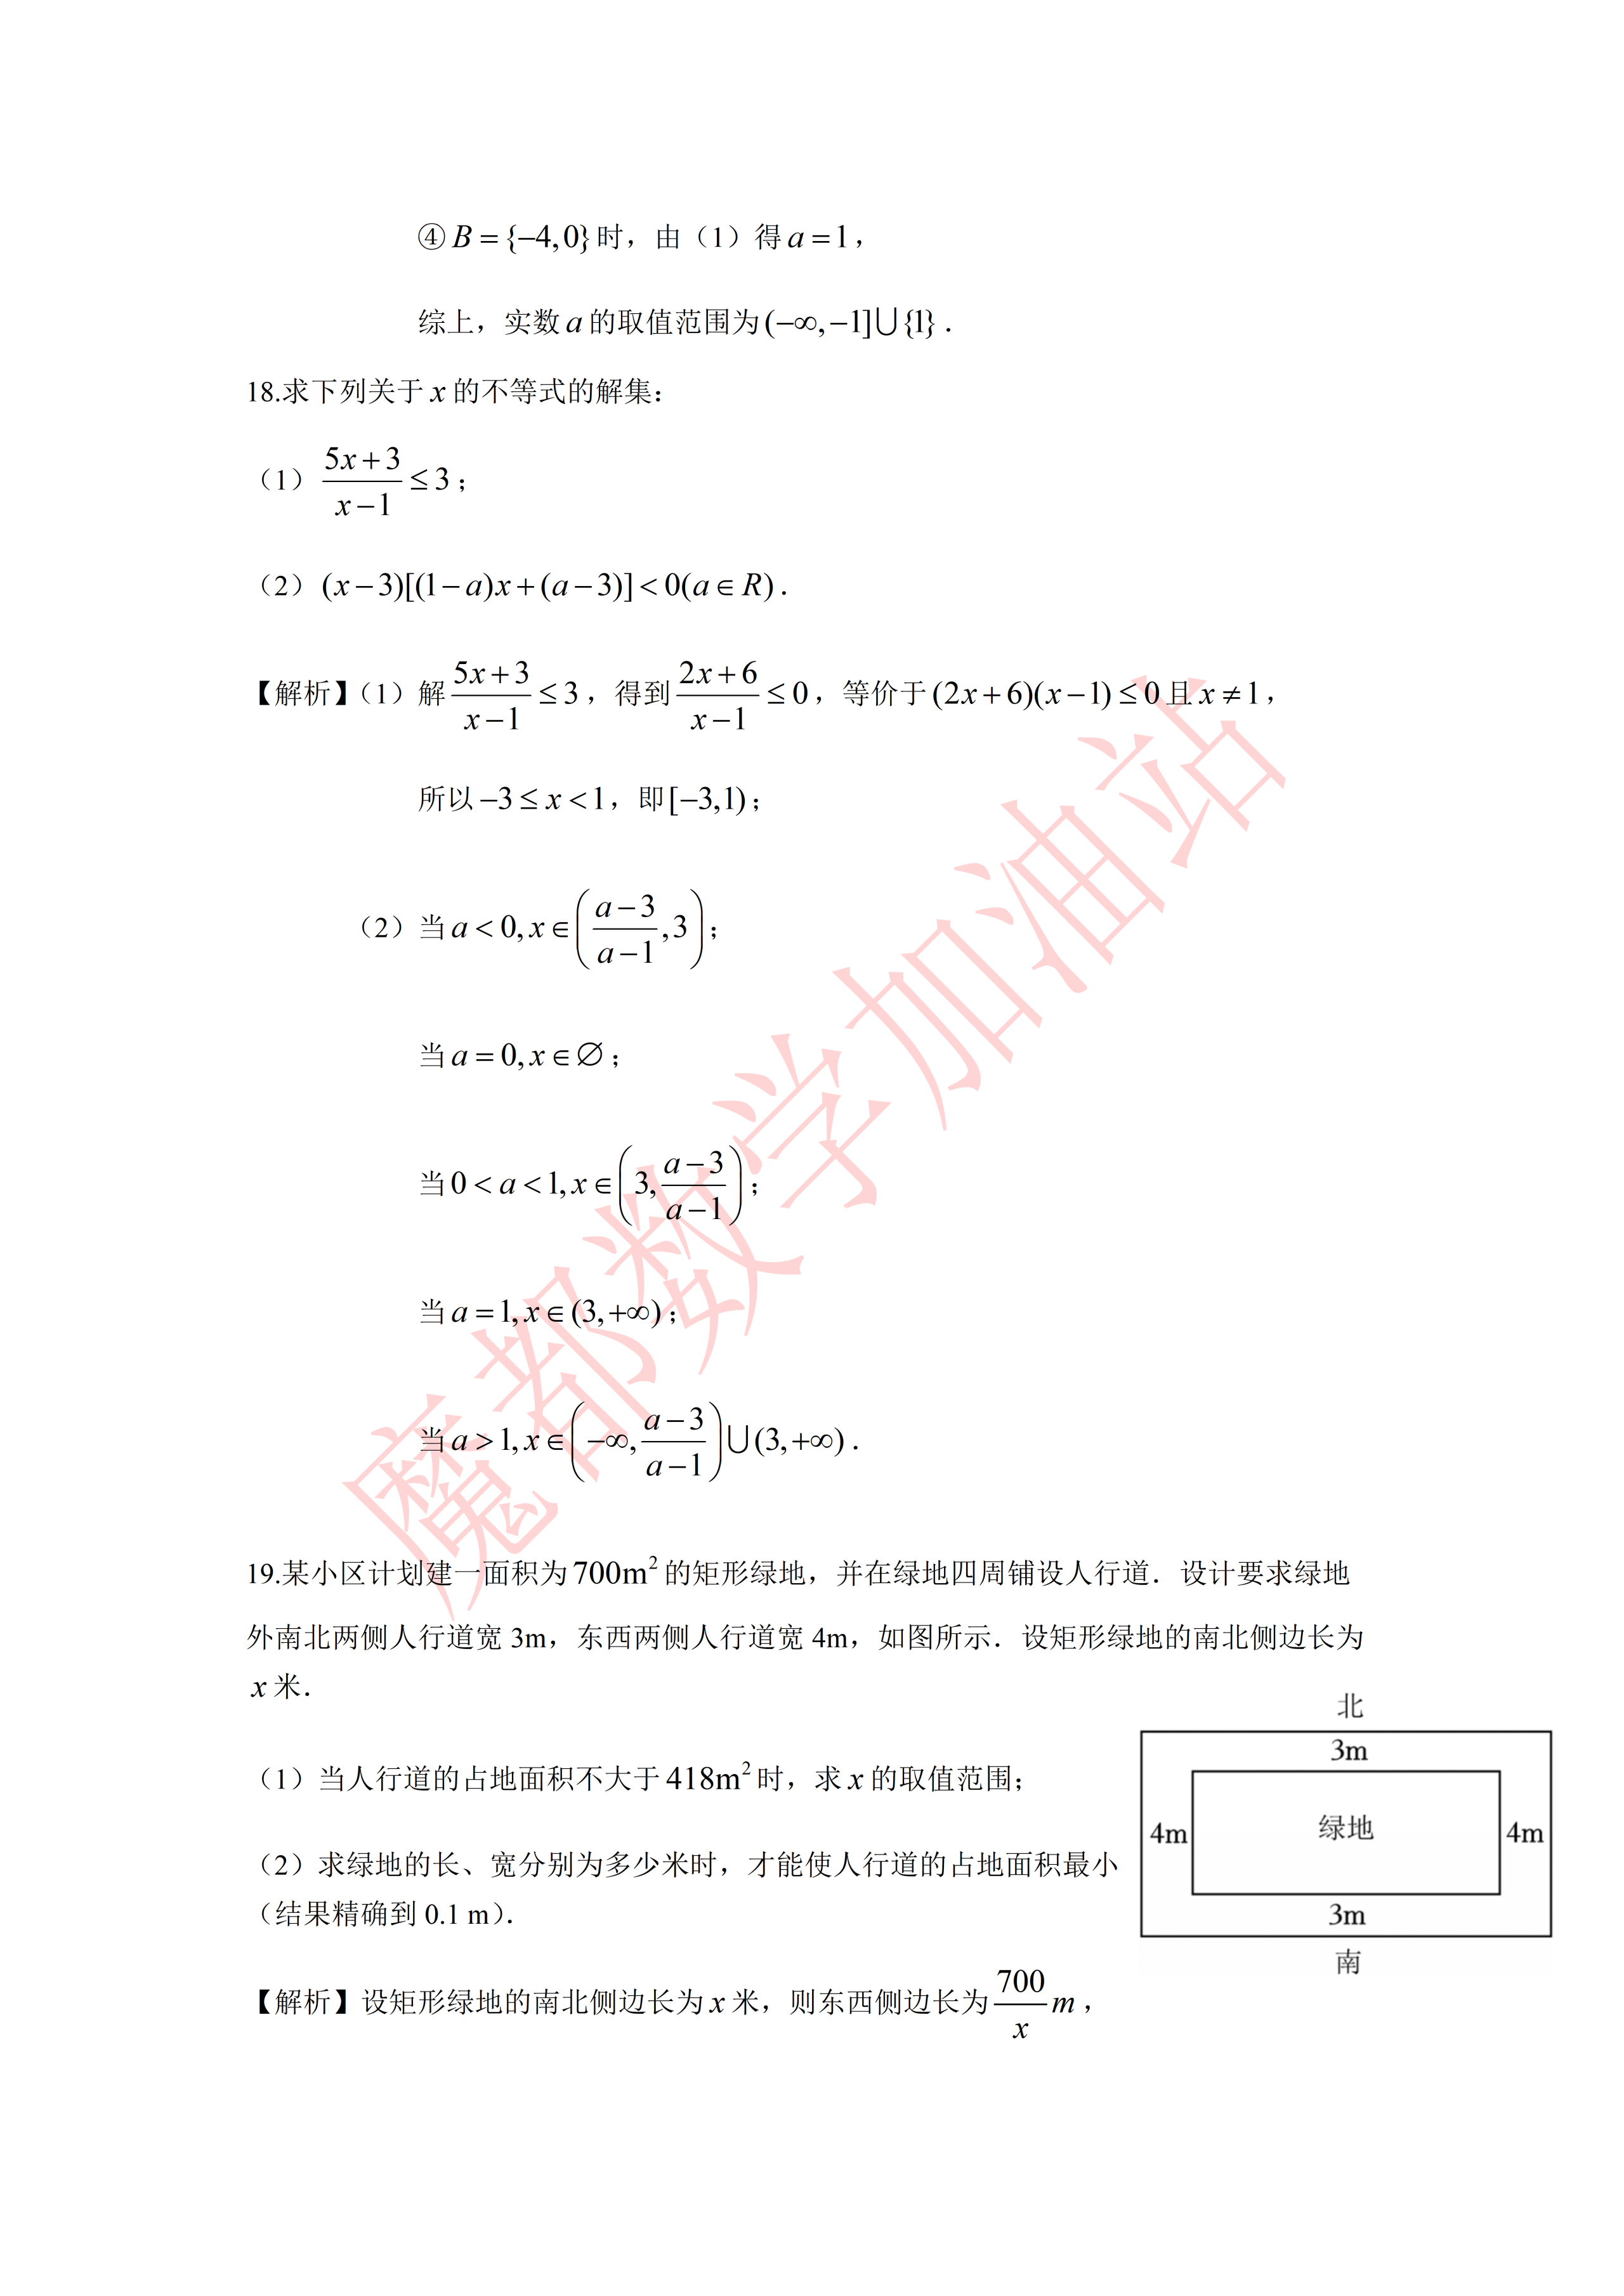
\includegraphics[width=.3\linewidth,trim=1791bp 484bp 107bp 2654bp,clip]{../原图/高一53_华师大二附中_10月月考/07.png}
\end{center}

\begin{enumerate}[label=(\arabic*)]
\item 当人行道的占地面积不大于 $418m^2$ 时，求 $x$ 的取值范围；
\item 求绿地的长、宽分别为多少米时，才能使人行道的占地面积最小（结果精确到 $0.1m$）.
\end{enumerate}

\ifanswer
\solbegin
\step{设矩形绿地的南北侧边长为 $x$ 米，则东西侧边长为 $\dfrac{700}{x}m$，}
\step{则人行道的占地面积为 $S=(x+8)\left(\dfrac{700}{x}+6\right)-700$，即 $S=6x+\dfrac{5600}{x}+48$.}
\stepm{(1)}{当人行道的占地面积不大于 $418m^2$ 时，$6x+\dfrac{5600}{x}+48\leqslant418$，}
\step{即 $6x^2-370x+5600\leqslant0$，解得 $\dfrac{80}{3}\leqslant x\leqslant35$，}
\step{故当人行道的占地面积不大于 $418m^2$ 时，$x\in\left[\dfrac{80}{3},35\right]$；}
\stepm{(2)}{$S=6x+\dfrac{5600}{x}+48\geqslant2\sqrt{6x\cdot\dfrac{5600}{x}}+48=80\sqrt{21}+48$，}
\step{当且仅当 $6x=\dfrac{5600}{x}$，即 $x=20\sqrt{\dfrac73}\approx30.6(m)$ 时，}
% 原卷如此，照录未改（80√21+48≈414.6，两处“414.4”疑笔误，见文件头“原卷笔误/存疑”第 6 条）
\step{$S$ 达到最小值 $80\sqrt{21}+48\approx414.4$，此时 $\dfrac{700}{x}\approx22.9(m)$，}
\step{所以当设计绿地的南北侧边长约为 $30.6m$，东西侧边长约为 $22.9m$ 时，}
\step{人行道的占地面积最小值为 $414.4(m^2)$.}
\solend
\fi

\ansspace[6]

\item 已知 $x\in\R$，符号 $[x]$ 表示不大于 $x$ 的最大整数，例如：$[2.3]=2$,$[2]=2$，$[-1.2]=-2$，令 $S(x)=[x]-[-x]$.

\begin{enumerate}[label=(\arabic*)]
\item 写出 $S(x)$ 为偶数（包括正、负偶数和 0）的充要条件，并证明；
\item 设方程 $|S(x)|=3$ 的解集为 $A$.

①集合 $B=\{x\mid x^2-ax-9\leqslant0,a\in\R\}$，若 $A\cap B=A$，求实数 $a$ 的取值范围；

②集合 $C=\{x\mid 2x^2-5kx+3k^2\geqslant0\}$，若 $A\cup C=\R$，求实数 $k$ 的取值范围.
\end{enumerate}

\ifanswer
\solbegin
\stepm{(1)}{$S(x)$ 为偶数的充要条件是 $x\in\Z$.}
\step{若 $x\in\Z$，则 $S(x)=[x]-[-x]=x-(-x)=2x$；}
\step{若 $x\notin\Z$，设 $[x]=n$，}
\step{则 $S(x)=[x]-[-x]=n-(-n-1)=2n+1=2[x]+1$；}
% 原卷如此，照录未改（“由①”按文意应为“由(1)”，见文件头“原卷笔误/存疑”第 3 条）
\stepm{(2)}{由①得 3 是奇数，$S(x)=\pm3$,$x\notin\Z$，}
\step{$S(x)=2[x]+1=\pm3$,$[x]=1$ 或 $-2$ 且 $x\notin\Z$，}
\step{所以 $A=(-2,-1)\cup(1,2)$；}
\stepm{①}{$A\cap B=A\Rightarrow A\subseteq B$，}
\step{设 $B=[x_1,x_2]$，其中 $x_1,x_2$ 是方程 $x^2-ax-9=0$ 的两实根，}
\step{设 $f(x)=x^2-ax-9$，}
\step{$[-2,2]\subseteq[x_1,x_2]\Leftrightarrow x_1\leqslant-2$,$x_2\geqslant2\Leftrightarrow\begin{cases}f(-2)\leqslant0\\ f(2)\leqslant0\end{cases}$}
\step{$\Leftrightarrow\begin{cases}(-2)^2-a\cdot(-2)-9\leqslant0, & a\leqslant\dfrac52\\ 2^2-2a-9\leqslant0, & a\geqslant-\dfrac52\end{cases}$，故 $a\in\left[-\dfrac52,\dfrac52\right]$；}
\step{注：若用求根公式 $\begin{cases}\dfrac{a+\sqrt{a^2+36}}{2}\geqslant2\Rightarrow a\geqslant-\dfrac52\\ \dfrac{a-\sqrt{a^2+36}}{2}\leqslant-2\Rightarrow a\leqslant\dfrac52\end{cases}$，结果正确，也得满分；}
\stepm{②}{$2x^2-5kx+3k^2=(x-k)(2x-3k)$.}
\step{$A\cup C=\R\Leftrightarrow\complement_\R A\subseteq C$.}
\step{记 $g(x)=2x^2-5kx+3k^2$，则 $\{x\mid g(x)<0\}\subseteq A$.}
\stepm{情况1：}{$k>0$ 时，$k<\dfrac32k$,$g(x)<0$ 的解集为 $\left(k,\dfrac32k\right)\subseteq(1,2)$，}
\step{故 $\begin{cases}k\geqslant1\\ \dfrac32k\leqslant2\end{cases}\Rightarrow1\leqslant k\leqslant\dfrac43$；}
\stepm{情况2：}{$k=0$ 时，$g(x)=2x^2\geqslant0$ 恒成立，$C=\R$,$A\cup C=\R$ 显然成立；}
\stepm{情况3：}{$k<0$ 时，$\dfrac32k<k$,$g(x)<0$ 的解集为 $\left(\dfrac32k,k\right)\subseteq(-2,-1)$，}
\step{故 $\begin{cases}\dfrac32k\geqslant-2\\ k\leqslant-1\end{cases}\Rightarrow-\dfrac43\leqslant k\leqslant-1$；}
\step{综上，$k\in\left[-\dfrac43,-1\right]\cup\{0\}\cup\left[1,\dfrac43\right]$.}
\solend
\fi

\ansspace[10]

\item 对于非空实数集 $M\subseteq(0,+\infty)$，若满足以下两个条件，则称 $M$ 为“极闭集”：

①$M$ 中至少含有 2 个元素，且 $1\notin M$；

②对于 $M$ 中任意两个不相等的元素 $x,y$，定义 $x*y=\dfrac{xy+1}{x+y}$，且 $x*y\in M$.

\begin{enumerate}[label=(\arabic*)]
\item 判断集合 $A=\left\{\dfrac12,2\right\}$ 与区间 $B=(1,+\infty)$ 是否为“极闭集”，并说明理由；
\item 若 $M$ 是“极闭集”，证明：集合 $M$ 中不可能所有元素都小于 1；
\item 证明：不存在任何有限的“极闭集”.
\end{enumerate}

\ifanswer
\solbegin
% 原卷如此，照录未改（首行集合按题干应为 {1/2,2}，见文件头“原卷笔误/存疑”第 7 条）
\stepm{(1)}{对于集合 $A=\left\{\dfrac12,1\right\}$，$\dfrac12*2=\dfrac45$，}
\step{因为 $\dfrac45\notin A$，不满足条件②，所以集合 $A$ 不是“极闭集”.}
\step{对于区间 $B$，满足条件①.}
\step{任取 $B$ 中两个不相等的元素 $x,y$，则 $x>1$,$y>1$.}
\step{$x*y-1=\dfrac{xy+1}{x+y}-1=\dfrac{(x-1)(y-1)}{x+y}>0$，所以 $x*y>1$，}
\step{这说明 $x*y\in B$ 恒成立，满足条件②，所以 $B$ 是“极闭集”.}
\stepm{(2)}{假设集合 $M$ 中所有元素都小于 1，}
\step{在 $M$ 中取 $0<x<y<1$,$x*y-1=\dfrac{xy+1}{x+y}-1=\dfrac{(x-1)(y-1)}{x+y}>0$，}
\step{所以 $x*y>1$，与“集合 $M$ 中所有元素都小于 1”矛盾，}
\step{假设不成立，集合 $M$ 中不可能所有元素都小于 1，得证.}
\stepm{(3)}{由②得，任何一个“极闭集”$M$ 中，必然至少存在一个大于 1 的元素，}
\stepm{情况1：}{若 $M$ 中至少存在两个大于 1 的元素，}
\step{设其中两个不相等的元素为 $x$ 和 $y_1$，且 $x>y_1>1$，}
\step{令 $y_{n+1}=x*y_n$,$n\geqslant1$,$y_{n+1}-1=x*y_n-1=\dfrac{(x-1)(y_n-1)}{xy_n+1}>0$，}
\step{如果 $y_n\geqslant1$，则显然 $y_{n+1}\geqslant1$，作差 $y_n-y_{n+1}=\dfrac{y_n^2-1}{x+y_n}>0$，}
\step{由此 $x>y_1>y_2>y_3>\cdots>1$，与有限集矛盾.}
\stepm{情况2：}{若 $M$ 中恰好只有一个元素大于 1，}
\step{设这个唯一大于 1 的元素为 $m$.}
\step{因为 $M$ 至少有两个元素，所以 $M$ 中必然至少存在一个元素 $a_1<1$，}
\step{令 $a_{n+1}=m*a_n$,$n\geqslant1$，}
\step{又 $a_{n+1}-1=m*a_n-1=\dfrac{(m-1)(a_n-1)}{m+a_n}<0$，故 $a_{n+1}<1$，}
\step{作差 $a_{n+1}-a_n=\dfrac{1-a_n^2}{m+a_n}>0$，由此 $a_1<a_2<a_3<\cdots<1$，与有限集矛盾.}
\step{因此，不存在任何有限的“极闭集”. 原命题得证.}
\solend
\fi

\ansspace*[10]

\end{enumerate}

\end{document}
"
% 紧凑版：xelatex "\def\iscompact{1}% 高一53_华师大二附中_10月月考.tex
%   —— 高一上数学“2026-2027 年华师大二附中高一上 10 月月考”（讲评版）
% 试卷版：xelatex 高一53_华师大二附中_10月月考.tex
% 答案版：xelatex "\def\isanswer{1}% 高一53_华师大二附中_10月月考.tex
%   —— 高一上数学“2026-2027 年华师大二附中高一上 10 月月考”（讲评版）
% 试卷版：xelatex 高一53_华师大二附中_10月月考.tex
% 答案版：xelatex "\def\isanswer{1}\input{高一53_华师大二附中_10月月考.tex}"
% 紧凑版：xelatex "\def\iscompact{1}\input{高一53_华师大二附中_10月月考.tex}"
%
% 原始材料：微信公众号“魔都数学加油站”文章，作者破晓，连载“27学年高一53”；
% 原文标题“27学年高一53——2026-2027年上海市华师大二附中高一上10月月考”；
% 原文链接：https://mp.weixin.qq.com/s/fpSnoF-gJEEWyxAoPC_bZA。
% 页面标注发布时间 2026-10-09 17:15（上海）。
% 正文为 11 张 PNG 页：第 01—06、08、10 页 4762×6735，第 07、09、11 页 2560×3620
% （**同一篇各页分辨率不同**），均按页序读取。11 页全为试卷正文页（卷首标题在第 1 页页顶，
% 卷末解答题第 21 题解析止于第 11 页），无封面页、目录页、二维码或宣传页。
% 粉色斜排“魔都数学加油站”为卷面水印，与公众号页脚一并未录入。
%
% 卷首标题：照卷面印作“2026--2027 年华师大二附中高一上 10 月月考”（公众号标题中的“上海市”
% 卷面标题行没有，本稿照卷面），年份区间按全稿惯例排 en dash。原卷只有一行标题、无副标题。
%
% 篇幅与题号：原卷自第 3 题起编号（第 1、2 题不在本卷内）。填空题 3—12（10 题）、
% 选择题 13—16（4 题）、解答题 17—21（5 题），共 19 题。本稿沿用原节与原题号，
% 只改排为全稿统一的大节样式（原卷小节标题为“一、填空题”“二、选择题”“三、解答题”）。
%
% 讲评版：原卷每题下直接印【答案】或【解析】。**第 13 题没有任何【答案】/【解析】段**，
% 答案“C”直接印在题干括号内（“一定不是(  C  )”），本稿按 高一37 第 13 题的成例把括号留空、
% 答案另提为 \ans{$C$}；其余 18 题都只印【解析】，按全稿口径这类题不另提 \ans{}——其中
% 选择题第 14、15、16 题的结论写在解析末句（“故选 B／D／C”），亦照录在解析内。
%
% 副标题：原卷未印副标题。本稿按“知识模块”口径标作“集合与常用逻辑用语、不等式”：
% 19 题中集合与常用逻辑用语 12 题（集合类 9 题——第 4、5、12、13、15、16、17、20、21 题；
% 逻辑类 3 题——第 3、9、14 题），不等式 7 题（含一元二次方程与绝对值方程：第 6、7、8、10、
% 11、18、19 题，其中第 11 题实为奇偶分析下的集合计数题，暂挂不等式），两类均超三分之一，
% 故并标。口径同 高一46、高一47、高一48、高一51、高一52。
%
% 与原卷的排版差异：
%   ① 原卷每题下直接印【解析】，本稿按全稿惯例将答案与解析置于答案版，试卷版保持干净；
%      第 13 题印在题干括号内的答案“C”同样移入 \ans{}，见上；
%   ② 原卷未印副标题，本稿按“知识模块”口径补出；
%   ③ 原卷填空横线约两个字宽，本稿按全稿惯例统一排 \blankline[4.4em]；
%      选择题的作答括号原卷排半角“(    )”，本稿按全稿惯例排 \mbox{（\quad）}；
%   ④ 原卷实数集排斜体/粗体 $R$、$\mathbf{R}$（第 4、6、7、18、20 题等处），本稿按全稿惯例
%      改用 $\R$；空集记号统一为 \varnothing；
%   ⑤ 原卷在数学式内多处用半角逗号（如 $x_1,x_2$、$|S|,|T|$、$a\neq0,c\neq0$），均照录未强改；
%      句末句点按全稿惯例排西文句点（原卷“故选 B．”一类全角句点亦从宽排作“.”）；
%   ⑥ 第 17—21 题的子问原卷各自另起一行，本稿按全稿惯例用 enumerate 的 (1)(2)(3)；
%      第 20 题 (2) 问下的①②两行是题干的一部分，照录为行首①②标号（不入 enumerate）；
%      解析中的子问标号一律用 \stepm{(1)}{…}，解析中的①②③④分情形用 \stepm{①}{…}；
%   ⑦ 第 12、20、21 题解析里的“情况1:”至“情况3:”标号原卷排**红色加粗**（全卷共 6 处），
%      全库无红色排字先例，本稿按全稿子题标号样式排 \stepm{情况1：}{…}（加粗着色、不改黑色基调），
%      冒号照原卷排全角；
%   ⑧ 第 19 题的示意图原卷排在题干右侧（与题干、(1) 问同高），本稿居中排在题干之后、
%      子问之前，并在 \item 前加 \needvspace 整块推走；图自原图第 07 页裁切（trim），不另存图片文件；
%   ⑨ 每道解答题原卷未留作答空白，本稿按全稿惯例加 \ansspace。
%
% 原卷笔误/存疑（均照录未改，正文对应处另有 % 注）：
%   1. 第 14 题解析末行“例如 $a=1$，$b=-1$，及必要性不成立”，“及”按文意应为“即”；
%   2. 第 15 题解析第 3 行 $\dfrac1{a+b\sqrt2}=\dfrac a{a^2-2b}+\left(-\dfrac b{a^2-2b}\right)\cdot\sqrt2$，
%      分母两处均作 $a^2-2b$，按通分应为 $a^2-2b^2$（结论 $C=X$ 不受影响）；
%   3. 第 20 题 (2) 问解析首行“由①得 3 是奇数”，按文意应为“由(1)得”（①是 (2) 问下自己
%      的子问标号，奇偶性结论出自 (1) 问）；
%   4. 第 11 题解析“只有奇数的有 $C_4^2+1=7$ 个”，按组合意义应为 $C_4^2+C_4^4=7$
%      （“$+1$”当指 4 个奇数全取的 1 种），数值无误；
%   5. 第 18 题 (2) 问解析“当 $a=0$,$x\in\varnothing$”，按文意应为“解集为 $\varnothing$”；
%   6. 第 19 题 (2) 问解析“$S$ 达到最小值 $80\sqrt{21}+48\approx414.4$”与末行
%      “人行道的占地面积最小值为 $414.4(m^2)$”，两处按 $80\sqrt{21}+48\approx414.6$，疑笔误；
%   7. 第 21 题 (1) 问解析首行“对于集合 $A=\left\{\frac12,1\right\}$”，按题干应为
%      $A=\left\{\frac12,2\right\}$（计算 $\frac12*2=\frac45$ 用的正是 $2$）；
%   8. 第 12 题解析“所以 $A=(-\infty,-4]\cup[2,+\infty)$”一行行末无标点，体例不一，照录。
%
% 插图：1 张，自原图裁切（无 \begin{tikzpicture} 重排）：
%   · 第 19 题绿地示意图（外矩形内套矩形“绿地”，上“北 3m”、下“南 3m”、左右各“4m”）
%     ——原图第 07 页，原卷排于题干右侧。
%     裁框：x 1797–2447、y 2660–3136（含“北”“南”标注，四周各留约 6px），
%     trim=1791bp 484bp 107bp 2654bp（左／下／右／上），页宽 2560、页高 3620。
%
\documentclass[a4paper,11pt]{article}
\usepackage{common}

\begin{document}

\examtitlest[3]{2026--2027 年华师大二附中高一上 10 月月考}{集合与常用逻辑用语、不等式}

\bigsec{一、填空题}

\begin{enumerate}
\setcounter{enumi}{2}

\item “$x=2$”是“$x^2-3x+2=0$”的\blankline[4.4em]条件.

（选择其中之一填空：充分非必要、必要非充分、充分、既非充分又非必要）

\ifanswer
\solbegin
\step{由 $x^2-3x+2=0$ 得 $x=1$ 或 $x=2$，}
\step{则“$x=2$”是“$x^2-3x+2=0$”的充分不必要条件.}
\solend
\fi

\item 已知 $R$ 是全集，集合 $A=\{y\mid y=-x^2+1,x\in\R\}$，集合 $B=\{x\mid x=3+|a|,a\in\R\}$，则 $\overline{A\cup B}=$\blankline[4.4em].

\ifanswer
\solbegin
\step{$A=\{y\mid y=-x^2+1,x\in\R\}=(-\infty,1]$，$B=\{x\mid x=3+|a|,a\in\R\}=[3,+\infty)$，}
\step{所以 $\overline{A\cup B}=(1,3)$.}
\solend
\fi

\item 已知 $a$ 为常数，集合 $A=\{x\mid x^2+x-6=0\}$，集合 $B=\{x\mid ax-2=0\}$，且 $B\subseteq A$，则 $a$ 的所有取值构成的集合为\blankline[4.4em].

\ifanswer
\solbegin
\step{集合 $A=\{-3,2\}$，因为 $B\subseteq A$，则 $B=\varnothing$，$\{-3\}$，$\{2\}$，$\{-3,2\}$，}
\step{当 $B=\varnothing$ 时，$a=0$，当 $B=\{-3\}$ 时，$a=-\dfrac23$，当 $B=\{2\}$ 时，$a=1$，}
\step{当 $B=\{-3,2\}$ 时，不成立，故 $a$ 的取值集合为 $\left\{0,-\dfrac23,1\right\}$.}
\solend
\fi

\item 设 $a\in\R$，若关于 $x$ 的不等式 $x^2-ax<0$ 的解集是区间 $(0,1)$ 的真子集，则 $a$ 的取值范围是\blankline[4.4em].

\ifanswer
\solbegin
\step{因为关于 $x$ 的不等式 $x^2-ax<0$ 的解集是区间 $(0,1)$ 的真子集，}
\step{当 $a=0$ 时，不等式的解集为 $\varnothing$，符合题意；}
\step{当 $a>0$ 时，不等式的解集为 $(0,a)$，则 $0<a<1$，}
\step{当 $a<0$ 时，不等式的解集为 $(a,0)$，不符合题意，}
\step{故 $a$ 的范围为 $[0,1)$.}
\solend
\fi

\item 设 $x\in\R$，则方程 $|2x+3|-|x-2|=|3x+1|$ 的解集为\blankline[4.4em].

\ifanswer
\solbegin
\step{当 $x\leqslant-\dfrac32$ 时，原式$\Leftrightarrow-2x-3+x-2=-3x-1\Leftrightarrow x=2$，不合题意；}
\step{当 $-\dfrac32<x\leqslant-\dfrac13$ 时，原式$\Leftrightarrow2x+3+x-2=-3x-1\Leftrightarrow x=-\dfrac13$；}
\step{当 $-\dfrac13<x\leqslant2$ 时，原式$\Leftrightarrow2x+3+x-2=3x+1\Leftrightarrow1=1$ 即恒成立；}
\step{当 $x>2$ 时，原式$\Leftrightarrow2x+3+2-x=3x+1\Leftrightarrow x=2$，不合题意；}
\step{故 $x\in\left[-\dfrac13,2\right]$.}
\solend
\fi

\item 已知关于 $x$ 的一元二次方程 $x^2+(4m+1)x+2m-1=0$．若方程的两根为 $x_1$、$x_2$，且满足 $\dfrac1{x_1}+\dfrac1{x_2}=-\dfrac12$，则实数 $m=$\blankline[4.4em].

\ifanswer
\solbegin
\step{由于判别式$\Delta=16m^2+5>0$恒成立，}
\step{不论 $m$ 为任何实数，方程总有两个不相等的实数根.}
\step{$\dfrac1{x_1}+\dfrac1{x_2}=-\dfrac12$，即 $\dfrac{x_1+x_2}{x_1x_2}=-\dfrac12$，由根与系数的关系得 $\dfrac{-4m-1}{2m-1}=-\dfrac12$，}
\step{解得 $m=-\dfrac12$.}
\solend
\fi

\item 已知 $\dfrac1{x-2}\geqslant1$ 是 $|x-a|<2$ 的充分非必要条件，则实数 $a$ 的取值范围是\blankline[4.4em].

\ifanswer
\solbegin
\step{由 $\dfrac1{x-2}\geqslant1$ 得 $\dfrac{3-x}{x-2}\geqslant0$，解得 $2<x\leqslant3$，由 $|x-a|<2$ 得 $a-2<x<a+2$，}
\step{因为 $\dfrac1{x-2}\geqslant1$ 是 $|x-a|<2$ 的充分非必要条件，}
\step{所以 $\{x\mid 2<x\leqslant3\}\subset\{x\mid a-2<x<a+2\}$，所以 $\begin{cases}a-2\leqslant2\\ a+2>3\end{cases}$，解得 $1<a\leqslant4$，}
\step{即实数 $a$ 的取值范围是 $(1,4]$.}
\solend
\fi

\item 设 $x,y\in(0,+\infty)$，且 $x+4y=1$，则 $\dfrac1x+\dfrac1y$ 的最小值为\blankline[4.4em].

\ifanswer
\solbegin
\step{因为 $\dfrac1x+\dfrac1y=(x+4y)\left(\dfrac1x+\dfrac1y\right)=5+\dfrac{4y}{x}+\dfrac{x}{y}\geqslant5+2\sqrt{\dfrac{4y}{x}\cdot\dfrac{x}{y}}=9$，}
\step{当且仅当 $\dfrac{4y}{x}=\dfrac{x}{y}$，即 $x=2y$，即 $x=\dfrac13$,$y=\dfrac16$ 时取等号，故最小值为 $9$.}
\solend
\fi

\item 设非空集合 $Q\subseteq M$，当 $Q$ 中所有元素和为偶数时（集合为单元素时和为元素本身），称 $Q$ 是 $M$ 的偶子集. 若集合 $M=\{1,2,3,4,5,6,7\}$，则其偶子集 $Q$ 的个数为\blankline[4.4em].

\ifanswer
\solbegin
\step{偶子集可以分为只有奇数、偶数及偶数个奇数和偶数的集合，}
\step{奇数有 4 个，偶数有 3 个，}
% 原卷如此，照录未改：按组合意义应为 C_4^2+C_4^4=7（“+1”当指 4 个奇数全取的 1 种），
% 见文件头“原卷笔误/存疑”第 4 条
\step{只有奇数的有 $C_4^2+1=7$ 个，只有偶数的有 $C_3^1+C_3^2+1=7$ 个，}
\step{偶数个奇数和偶数的：两奇一偶 $C_4^2\cdot C_3^1=18$ 个，两奇二偶 $C_4^2\cdot C_3^2=18$ 个，}
\step{两奇三偶 $C_4^2\cdot C_3^3=6$ 个，四奇一偶 $C_4^4\cdot C_3^1=3$ 个，四奇二偶 $C_4^4\cdot C_3^2=3$ 个，}
\step{四奇三偶 $C_4^4\cdot C_3^3=1$ 个，所以共有 $7+7+18+18+6+3+3+1=63$ 个.}
\solend
\fi

\item 已知集合 $A=\{x\mid x^2+2x-8\geqslant0\}$,$B=\{x\mid x^2-2ax+2a\leqslant0\}$，且 $A\cap B$ 中恰有 3 个整数元素，则实数 $a$ 的取值范围为\blankline[4.4em].

\ifanswer
\solbegin
% 原卷如此，照录未改：此行行末无标点，见文件头“原卷笔误/存疑”第 8 条
\step{由 $x^2+2x-8\geqslant0$，得 $x\geqslant2$ 或 $x\leqslant-4$，所以 $A=(-\infty,-4]\cup[2,+\infty)$}
\step{对集合 $B$：$x^2-2ax+2a\leqslant0$,$\Delta=4a^2-8a=4a(a-2)\geqslant0$，}
\step{得 $a\leqslant0$ 或 $a\geqslant2$.}
\step{设方程 $x^2-2ax+2a=0$ 的两根为 $r_1,r_2$，}
\step{则 $B=[r_1,r_2]$,$r_1=a-\sqrt{a^2-2a}$,$r_2=a+\sqrt{a^2-2a}$，}
\stepm{情况1：}{$a\leqslant0$，}
\step{$r_2=a+\sqrt{a^2-2a}<a+\sqrt{a^2-2a+1}=a+|a-1|=a+1-a=1<2$，}
\step{$B$ 只在 $A$ 的左侧部分有交集，要使 $A\cap B$ 恰有 3 个整数元素，}
\step{这 3 个整数为 $-6,-5,-4$，于是 $r_1\in(-7,-6]$，}
\step{令 $f(x)=x^2-2ax+2a$，则 $\begin{cases}f(-7)=49+14a+2a>0\\ f(-6)=36+12a+2a\leqslant0\end{cases}\Rightarrow a\in\left(-\dfrac{49}{16},-\dfrac{18}{7}\right]$；}
\stepm{情况2：}{$a\geqslant2$，}
\step{$r_2=a+\sqrt{a^2-2a}\geqslant2$，}
\step{$r_1=a-\sqrt{a^2-2a}>a-\sqrt{a^2-2a+1}=a-|a-1|=a-(a-1)=1>-4$，}
\step{所以 $A\cap B=[2,r_2]$.}
\step{同理 $\begin{cases}f(4)=16-8a+2a\leqslant0\\ f(5)=25-10a+2a>0\end{cases}\Rightarrow a\in\left[\dfrac{8}{3},\dfrac{25}{8}\right)$；}
\step{综上，$a\in\left(-\dfrac{49}{16},-\dfrac{18}{7}\right]\cup\left[\dfrac{8}{3},\dfrac{25}{8}\right)$.}
\solend
\fi

\end{enumerate}

\bigsec{二、选择题}

\begin{enumerate}
\setcounter{enumi}{12}

% 第 13 题原卷无【答案】/【解析】段，答案“C”直接印在题干括号内，
% 按高一37 第 13 题的成例括号留空、答案另提为 \ans{}（见文件头）
\item 集合 $A=\{a,b,c\}$ 中的三个元素分别表示某一个三角形的三边长度，那么这个三角形一定不是\mbox{（\quad）}

\keepwithprev
A. 锐角三角形\qquad B. 钝角三角形

C. 等腰三角形\qquad D. 直角三角形

\ifanswer
\ans{$C$}
\fi

\item 设 $a$、$b$ 为实数，则“$a<b<0$”是“$\dfrac1a>\dfrac1b$”的\mbox{（\quad）}条件.

\keepwithprev
A. 充要\qquad B. 充分不必要

C. 必要不充分\qquad D. 既不充分也不必要

\ifanswer
\solbegin
\step{若 $a<b<0$，则 $\dfrac1a>\dfrac1b$ 一定成立，即充分性成立；}
% 原卷如此，照录未改（“及”按文意应为“即”，见文件头“原卷笔误/存疑”第 1 条）
\step{若 $\dfrac1a>\dfrac1b$ 成立，$a<b<0$ 不一定成立，例如 $a=1$，$b=-1$，及必要性不成立.}
\step{故选 $B$.}
\solend
\fi

\item 设 $Q$ 表示有理数集，集合 $X=\{x\mid x=a+b\sqrt2,a,b\in Q,x\neq0\}$，在下列集合中：①$\{2x\mid x\in X\}$②$\left\{\dfrac{x}{\sqrt2}\mid x\in X\right\}$③$\left\{\dfrac1x\mid x\in X\right\}$④$\{x^2\mid x\in X\}$，与 $X$ 相同的集合有\mbox{（\quad）}

\keepwithprev
A. ①②③④\qquad B. ②③④\qquad C. ①②④\qquad D. ①②③

\ifanswer
\solbegin
\step{$A=\{2x\mid x\in X\}$，$2(a+b\sqrt2)=p+q\sqrt2$ 得 $p=2a$，$q=2b$，$a=\dfrac p2$，$b=\dfrac q2$，}
\step{也是一一对应，$A=X$}
% 原卷如此，照录未改：分母两处均作 a^2-2b，按通分应为 a^2-2b^2，
% 见文件头“原卷笔误/存疑”第 2 条
\step{集合 $B=\left\{\dfrac{x}{\sqrt2}\mid x\in X\right\}$，$\dfrac{a+b\sqrt2}{\sqrt2}=b+\dfrac a2\cdot\sqrt2$，也是一一对应，$B=X$}
\step{集合 $C=\left\{\dfrac1x\mid x\in X\right\}$，$\dfrac{1}{a+b\sqrt2}=\dfrac{a}{a^2-2b}+\left(-\dfrac{b}{a^2-2b}\right)\cdot\sqrt2$，一一对应，$C=X$}
\step{集合 $D=\{x^2\mid x\in X\}$，$(a+b\sqrt2)^2=a^2+2b^2+2ab\sqrt2$，这个不能一一对应了，}
\step{集合 $D$ 包含于 $X$ 中.}
\step{故 $X$ 相同的集合有①②③，故选 $D$.}
\solend
\fi

\item 集合 $S=\{x\mid(x+a)(x^2+bx+c)=0\}$,$T=\{x\mid(ax+1)(cx^2+bx+1)=0\}$，其中 $a,b,c$ 为实数，若 $|S|,|T|$ 分别表示集合 $S,T$ 的元素个数，则 $|S|-|T|$ 的所有可能取值集合为\mbox{（\quad）}

\keepwithprev
A. $\{0\}$\qquad B. $\{1\}$\qquad C. $\{0,1\}$\qquad D. $\{-1,0,1\}$

\ifanswer
\solbegin
\stepm{①}{$a\neq0,c\neq0$ 时.}
\step{$S$ 中 $x+a=0$ 的根 $x=-a$;$T$ 中 $ax+1=0$ 的根 $x=-\dfrac1a$.}
\step{$S$ 中的 $x^2+bx+c=0$ 若无实根，则 $T$ 中的 $cx^2+bx+1=0$ 也无实根；}
\step{又设 $S$ 的 $x^2+bx+c=0$ 的根为 $r(r\neq0)$，则 $T$ 的 $cx^2+bx+1=0$ 的根为 $\dfrac1r$.}
\step{（因为 $r^2+br+c=0\Rightarrow c\cdot\left(\dfrac1r\right)^2+b\cdot\dfrac1r+1=0$）}
\step{即 $a\neq0,c\neq0$ 时，}
\step{$S$ 与 $T$ 的实根存在一一对应关系 $x\leftrightarrow\dfrac1x$,$|S|=|T|,$$|S|-|T|=0$；}
\stepm{②}{$a=0,c\neq0$ 时.}
\step{$S$ 中多出一个根 $x=0$，而 $T$ 中无此根，$|S|=|T|+1$，即 $|S|-|T|=1$；}
\stepm{③}{$a\neq0,c=0$ 时.}
\step{则 $S$ 中仍有根 $x=0$，而 $T$ 中无 0 根，同样 $|S|-|T|=1$.}
\stepm{④}{$a=0,c=0$ 时.}
\step{同样 $S$ 含有根 0，而 $T$ 中不含 0，仍有 $|S|-|T|=1$.}
\step{综上，$|S|-|T|$ 所有可能取值为 0 和 1，故选 $C$.}
\solend
\fi

\end{enumerate}

\bigsec{三、解答题}

\begin{enumerate}
\setcounter{enumi}{16}

\item 已知集合 $A=\{x\mid x^2+4x=0\}$，$B=\{x\mid x^2+2(a+1)x+a^2-1=0\}$.

\begin{enumerate}[label=(\arabic*)]
\item 若 $A$ 是 $B$ 的子集，求实数 $a$ 的值；
\item 若 $B$ 是 $A$ 的子集，求实数 $a$ 的取值范围.
\end{enumerate}

\ifanswer
\solbegin
\stepm{(1)}{因为 $A=\{-4,0\}$，$B=\{x\mid x^2+2(a+1)x+a^2-1=0\}$，又 $A\subseteq B$，}
\step{所以 $A=B$，所以 $\begin{cases}-4+0=-2(a+1)\\ -4\times0=a^2-1\end{cases}$，所以 $a=1$；}
\stepm{(2)}{因为 $B$ 是 $A$ 的子集，所以 $B=\varnothing$ 或 $B=\{-4\}$ 或 $B=\{0\}$ 或 $B=\{-4,0\}$，}
\stepm{①}{$B=\varnothing$ 时，$\Delta=4(a+1)^2-4(a^2-1)<0$，所以 $a<-1$；}
\stepm{②}{$B=\{-4\}$ 时，$\begin{cases}-4+(-4)=-2(a+1)\\ -4\times(-4)=a^2-1\end{cases}$，无解；}
\stepm{③}{$B=\{0\}$ 时，$\begin{cases}0+0=-2(a+1)\\ 0\times0=a^2-1\end{cases}$，所以 $a=-1$；}
\stepm{④}{$B=\{-4,0\}$ 时，由（1）得 $a=1$，}
\step{综上，实数 $a$ 的取值范围为 $(-\infty,-1]\cup\{1\}$.}
\solend
\fi

\ansspace[6]

\item 求下列关于 $x$ 的不等式的解集：

\begin{enumerate}[label=(\arabic*)]
\item $\dfrac{5x+3}{x-1}\leqslant3$；
\item $(x-3)[(1-a)x+(a-3)]<0$ ($a\in\R$).
\end{enumerate}

\ifanswer
\solbegin
\stepm{(1)}{解 $\dfrac{5x+3}{x-1}\leqslant3$，得到 $\dfrac{2x+6}{x-1}\leqslant0$，等价于 $(2x+6)(x-1)\leqslant0$ 且 $x\neq1$，}
\step{所以 $-3\leqslant x<1$，即 $[-3,1)$；}
\stepm{(2)}{当 $a<0$,$x\in\left(\dfrac{a-3}{a-1},3\right)$；}
% 原卷如此，照录未改（“x∈∅”按文意应为“解集为 ∅”，见文件头“原卷笔误/存疑”第 5 条）
\step{当 $a=0$,$x\in\varnothing$；}
\step{当 $0<a<1$,$x\in\left(3,\dfrac{a-3}{a-1}\right)$；}
\step{当 $a=1$,$x\in(3,+\infty)$；}
\step{当 $a>1$,$x\in\left(-\infty,\dfrac{a-3}{a-1}\right)\cup(3,+\infty)$.}
\solend
\fi

\ansspace[6]

\needvspace{13\baselineskip}

\item 某小区计划建一面积为 $700m^2$ 的矩形绿地，并在绿地四周铺设人行道. 设计要求绿地外南北两侧人行道宽 $3m$，东西两侧人行道宽 $4m$，如图所示. 设矩形绿地的南北侧边长为 $x$ 米.

\begin{center}
% 原图第 7 页题干绿地示意图直接裁取（原卷排于题干右侧）。
% 裁框取图形外框 x 1797–2447、y 2660–3136（含“北”“南”标注，四周各留约 6px），
% trim=左 1791bp／下 484bp／右 107bp／上 2654bp（页宽 2560、页高 3620）。
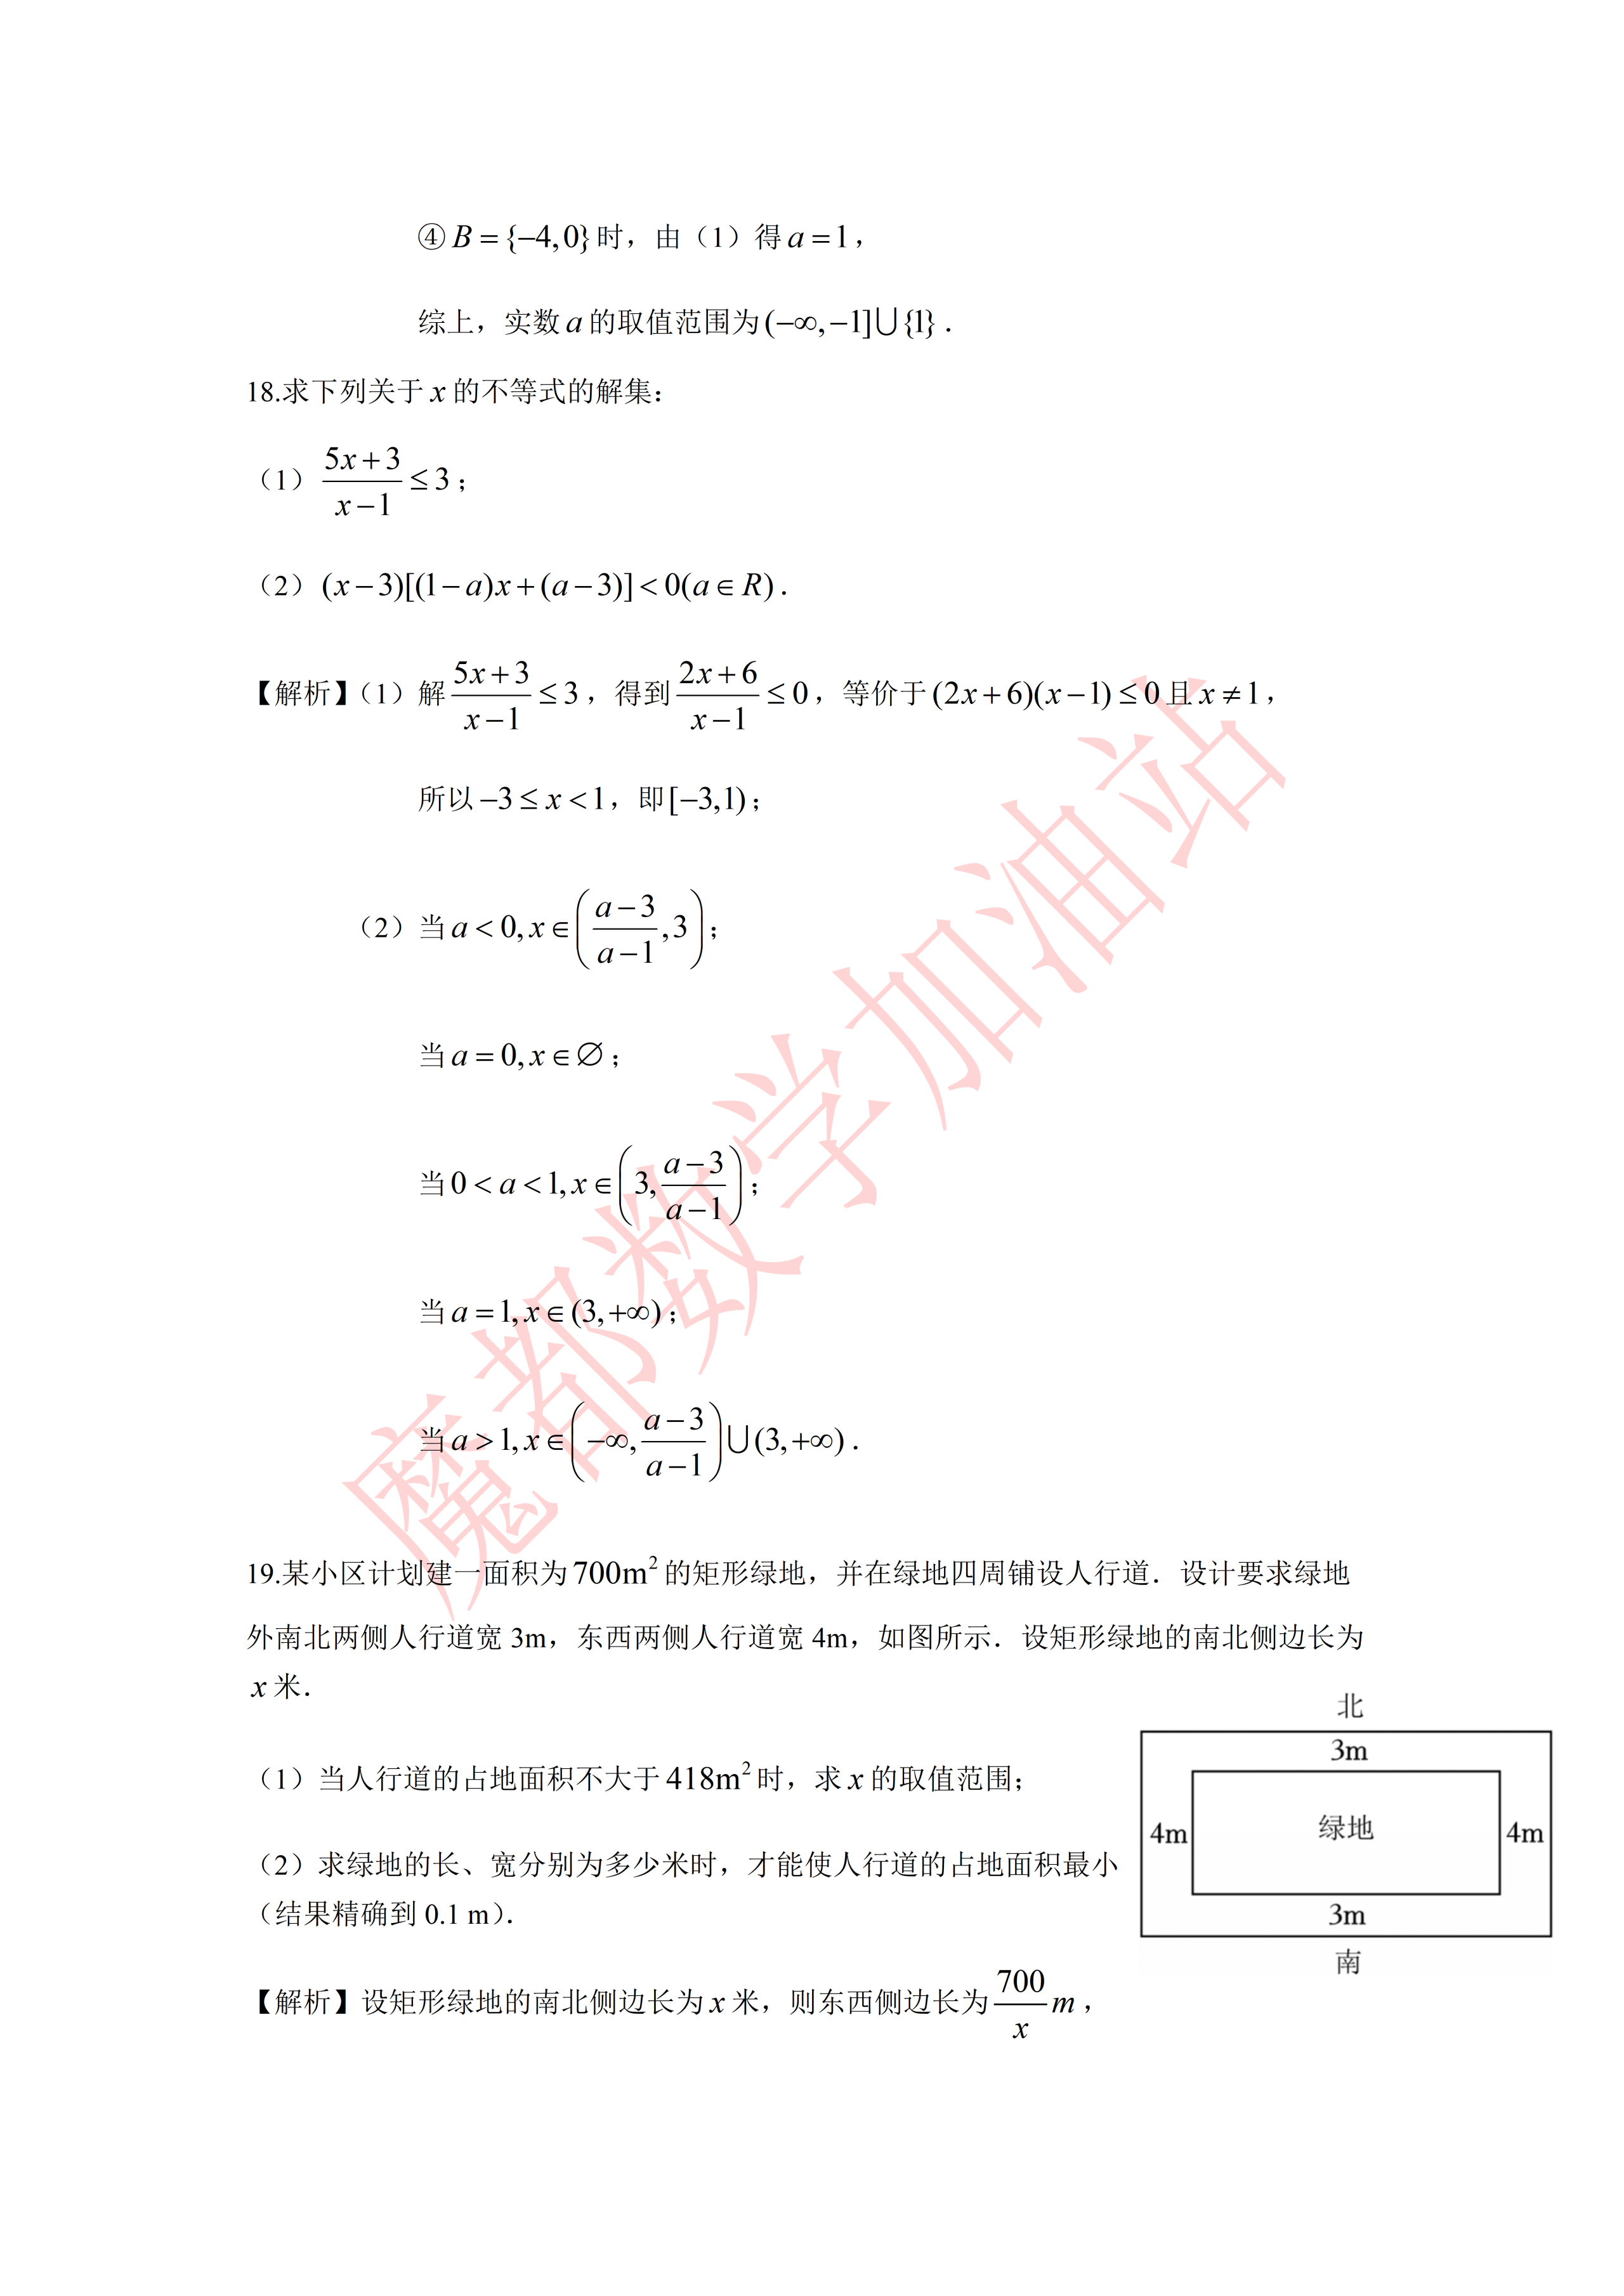
\includegraphics[width=.3\linewidth,trim=1791bp 484bp 107bp 2654bp,clip]{../原图/高一53_华师大二附中_10月月考/07.png}
\end{center}

\begin{enumerate}[label=(\arabic*)]
\item 当人行道的占地面积不大于 $418m^2$ 时，求 $x$ 的取值范围；
\item 求绿地的长、宽分别为多少米时，才能使人行道的占地面积最小（结果精确到 $0.1m$）.
\end{enumerate}

\ifanswer
\solbegin
\step{设矩形绿地的南北侧边长为 $x$ 米，则东西侧边长为 $\dfrac{700}{x}m$，}
\step{则人行道的占地面积为 $S=(x+8)\left(\dfrac{700}{x}+6\right)-700$，即 $S=6x+\dfrac{5600}{x}+48$.}
\stepm{(1)}{当人行道的占地面积不大于 $418m^2$ 时，$6x+\dfrac{5600}{x}+48\leqslant418$，}
\step{即 $6x^2-370x+5600\leqslant0$，解得 $\dfrac{80}{3}\leqslant x\leqslant35$，}
\step{故当人行道的占地面积不大于 $418m^2$ 时，$x\in\left[\dfrac{80}{3},35\right]$；}
\stepm{(2)}{$S=6x+\dfrac{5600}{x}+48\geqslant2\sqrt{6x\cdot\dfrac{5600}{x}}+48=80\sqrt{21}+48$，}
\step{当且仅当 $6x=\dfrac{5600}{x}$，即 $x=20\sqrt{\dfrac73}\approx30.6(m)$ 时，}
% 原卷如此，照录未改（80√21+48≈414.6，两处“414.4”疑笔误，见文件头“原卷笔误/存疑”第 6 条）
\step{$S$ 达到最小值 $80\sqrt{21}+48\approx414.4$，此时 $\dfrac{700}{x}\approx22.9(m)$，}
\step{所以当设计绿地的南北侧边长约为 $30.6m$，东西侧边长约为 $22.9m$ 时，}
\step{人行道的占地面积最小值为 $414.4(m^2)$.}
\solend
\fi

\ansspace[6]

\item 已知 $x\in\R$，符号 $[x]$ 表示不大于 $x$ 的最大整数，例如：$[2.3]=2$,$[2]=2$，$[-1.2]=-2$，令 $S(x)=[x]-[-x]$.

\begin{enumerate}[label=(\arabic*)]
\item 写出 $S(x)$ 为偶数（包括正、负偶数和 0）的充要条件，并证明；
\item 设方程 $|S(x)|=3$ 的解集为 $A$.

①集合 $B=\{x\mid x^2-ax-9\leqslant0,a\in\R\}$，若 $A\cap B=A$，求实数 $a$ 的取值范围；

②集合 $C=\{x\mid 2x^2-5kx+3k^2\geqslant0\}$，若 $A\cup C=\R$，求实数 $k$ 的取值范围.
\end{enumerate}

\ifanswer
\solbegin
\stepm{(1)}{$S(x)$ 为偶数的充要条件是 $x\in\Z$.}
\step{若 $x\in\Z$，则 $S(x)=[x]-[-x]=x-(-x)=2x$；}
\step{若 $x\notin\Z$，设 $[x]=n$，}
\step{则 $S(x)=[x]-[-x]=n-(-n-1)=2n+1=2[x]+1$；}
% 原卷如此，照录未改（“由①”按文意应为“由(1)”，见文件头“原卷笔误/存疑”第 3 条）
\stepm{(2)}{由①得 3 是奇数，$S(x)=\pm3$,$x\notin\Z$，}
\step{$S(x)=2[x]+1=\pm3$,$[x]=1$ 或 $-2$ 且 $x\notin\Z$，}
\step{所以 $A=(-2,-1)\cup(1,2)$；}
\stepm{①}{$A\cap B=A\Rightarrow A\subseteq B$，}
\step{设 $B=[x_1,x_2]$，其中 $x_1,x_2$ 是方程 $x^2-ax-9=0$ 的两实根，}
\step{设 $f(x)=x^2-ax-9$，}
\step{$[-2,2]\subseteq[x_1,x_2]\Leftrightarrow x_1\leqslant-2$,$x_2\geqslant2\Leftrightarrow\begin{cases}f(-2)\leqslant0\\ f(2)\leqslant0\end{cases}$}
\step{$\Leftrightarrow\begin{cases}(-2)^2-a\cdot(-2)-9\leqslant0, & a\leqslant\dfrac52\\ 2^2-2a-9\leqslant0, & a\geqslant-\dfrac52\end{cases}$，故 $a\in\left[-\dfrac52,\dfrac52\right]$；}
\step{注：若用求根公式 $\begin{cases}\dfrac{a+\sqrt{a^2+36}}{2}\geqslant2\Rightarrow a\geqslant-\dfrac52\\ \dfrac{a-\sqrt{a^2+36}}{2}\leqslant-2\Rightarrow a\leqslant\dfrac52\end{cases}$，结果正确，也得满分；}
\stepm{②}{$2x^2-5kx+3k^2=(x-k)(2x-3k)$.}
\step{$A\cup C=\R\Leftrightarrow\complement_\R A\subseteq C$.}
\step{记 $g(x)=2x^2-5kx+3k^2$，则 $\{x\mid g(x)<0\}\subseteq A$.}
\stepm{情况1：}{$k>0$ 时，$k<\dfrac32k$,$g(x)<0$ 的解集为 $\left(k,\dfrac32k\right)\subseteq(1,2)$，}
\step{故 $\begin{cases}k\geqslant1\\ \dfrac32k\leqslant2\end{cases}\Rightarrow1\leqslant k\leqslant\dfrac43$；}
\stepm{情况2：}{$k=0$ 时，$g(x)=2x^2\geqslant0$ 恒成立，$C=\R$,$A\cup C=\R$ 显然成立；}
\stepm{情况3：}{$k<0$ 时，$\dfrac32k<k$,$g(x)<0$ 的解集为 $\left(\dfrac32k,k\right)\subseteq(-2,-1)$，}
\step{故 $\begin{cases}\dfrac32k\geqslant-2\\ k\leqslant-1\end{cases}\Rightarrow-\dfrac43\leqslant k\leqslant-1$；}
\step{综上，$k\in\left[-\dfrac43,-1\right]\cup\{0\}\cup\left[1,\dfrac43\right]$.}
\solend
\fi

\ansspace[10]

\item 对于非空实数集 $M\subseteq(0,+\infty)$，若满足以下两个条件，则称 $M$ 为“极闭集”：

①$M$ 中至少含有 2 个元素，且 $1\notin M$；

②对于 $M$ 中任意两个不相等的元素 $x,y$，定义 $x*y=\dfrac{xy+1}{x+y}$，且 $x*y\in M$.

\begin{enumerate}[label=(\arabic*)]
\item 判断集合 $A=\left\{\dfrac12,2\right\}$ 与区间 $B=(1,+\infty)$ 是否为“极闭集”，并说明理由；
\item 若 $M$ 是“极闭集”，证明：集合 $M$ 中不可能所有元素都小于 1；
\item 证明：不存在任何有限的“极闭集”.
\end{enumerate}

\ifanswer
\solbegin
% 原卷如此，照录未改（首行集合按题干应为 {1/2,2}，见文件头“原卷笔误/存疑”第 7 条）
\stepm{(1)}{对于集合 $A=\left\{\dfrac12,1\right\}$，$\dfrac12*2=\dfrac45$，}
\step{因为 $\dfrac45\notin A$，不满足条件②，所以集合 $A$ 不是“极闭集”.}
\step{对于区间 $B$，满足条件①.}
\step{任取 $B$ 中两个不相等的元素 $x,y$，则 $x>1$,$y>1$.}
\step{$x*y-1=\dfrac{xy+1}{x+y}-1=\dfrac{(x-1)(y-1)}{x+y}>0$，所以 $x*y>1$，}
\step{这说明 $x*y\in B$ 恒成立，满足条件②，所以 $B$ 是“极闭集”.}
\stepm{(2)}{假设集合 $M$ 中所有元素都小于 1，}
\step{在 $M$ 中取 $0<x<y<1$,$x*y-1=\dfrac{xy+1}{x+y}-1=\dfrac{(x-1)(y-1)}{x+y}>0$，}
\step{所以 $x*y>1$，与“集合 $M$ 中所有元素都小于 1”矛盾，}
\step{假设不成立，集合 $M$ 中不可能所有元素都小于 1，得证.}
\stepm{(3)}{由②得，任何一个“极闭集”$M$ 中，必然至少存在一个大于 1 的元素，}
\stepm{情况1：}{若 $M$ 中至少存在两个大于 1 的元素，}
\step{设其中两个不相等的元素为 $x$ 和 $y_1$，且 $x>y_1>1$，}
\step{令 $y_{n+1}=x*y_n$,$n\geqslant1$,$y_{n+1}-1=x*y_n-1=\dfrac{(x-1)(y_n-1)}{xy_n+1}>0$，}
\step{如果 $y_n\geqslant1$，则显然 $y_{n+1}\geqslant1$，作差 $y_n-y_{n+1}=\dfrac{y_n^2-1}{x+y_n}>0$，}
\step{由此 $x>y_1>y_2>y_3>\cdots>1$，与有限集矛盾.}
\stepm{情况2：}{若 $M$ 中恰好只有一个元素大于 1，}
\step{设这个唯一大于 1 的元素为 $m$.}
\step{因为 $M$ 至少有两个元素，所以 $M$ 中必然至少存在一个元素 $a_1<1$，}
\step{令 $a_{n+1}=m*a_n$,$n\geqslant1$，}
\step{又 $a_{n+1}-1=m*a_n-1=\dfrac{(m-1)(a_n-1)}{m+a_n}<0$，故 $a_{n+1}<1$，}
\step{作差 $a_{n+1}-a_n=\dfrac{1-a_n^2}{m+a_n}>0$，由此 $a_1<a_2<a_3<\cdots<1$，与有限集矛盾.}
\step{因此，不存在任何有限的“极闭集”. 原命题得证.}
\solend
\fi

\ansspace*[10]

\end{enumerate}

\end{document}
"
% 紧凑版：xelatex "\def\iscompact{1}% 高一53_华师大二附中_10月月考.tex
%   —— 高一上数学“2026-2027 年华师大二附中高一上 10 月月考”（讲评版）
% 试卷版：xelatex 高一53_华师大二附中_10月月考.tex
% 答案版：xelatex "\def\isanswer{1}\input{高一53_华师大二附中_10月月考.tex}"
% 紧凑版：xelatex "\def\iscompact{1}\input{高一53_华师大二附中_10月月考.tex}"
%
% 原始材料：微信公众号“魔都数学加油站”文章，作者破晓，连载“27学年高一53”；
% 原文标题“27学年高一53——2026-2027年上海市华师大二附中高一上10月月考”；
% 原文链接：https://mp.weixin.qq.com/s/fpSnoF-gJEEWyxAoPC_bZA。
% 页面标注发布时间 2026-10-09 17:15（上海）。
% 正文为 11 张 PNG 页：第 01—06、08、10 页 4762×6735，第 07、09、11 页 2560×3620
% （**同一篇各页分辨率不同**），均按页序读取。11 页全为试卷正文页（卷首标题在第 1 页页顶，
% 卷末解答题第 21 题解析止于第 11 页），无封面页、目录页、二维码或宣传页。
% 粉色斜排“魔都数学加油站”为卷面水印，与公众号页脚一并未录入。
%
% 卷首标题：照卷面印作“2026--2027 年华师大二附中高一上 10 月月考”（公众号标题中的“上海市”
% 卷面标题行没有，本稿照卷面），年份区间按全稿惯例排 en dash。原卷只有一行标题、无副标题。
%
% 篇幅与题号：原卷自第 3 题起编号（第 1、2 题不在本卷内）。填空题 3—12（10 题）、
% 选择题 13—16（4 题）、解答题 17—21（5 题），共 19 题。本稿沿用原节与原题号，
% 只改排为全稿统一的大节样式（原卷小节标题为“一、填空题”“二、选择题”“三、解答题”）。
%
% 讲评版：原卷每题下直接印【答案】或【解析】。**第 13 题没有任何【答案】/【解析】段**，
% 答案“C”直接印在题干括号内（“一定不是(  C  )”），本稿按 高一37 第 13 题的成例把括号留空、
% 答案另提为 \ans{$C$}；其余 18 题都只印【解析】，按全稿口径这类题不另提 \ans{}——其中
% 选择题第 14、15、16 题的结论写在解析末句（“故选 B／D／C”），亦照录在解析内。
%
% 副标题：原卷未印副标题。本稿按“知识模块”口径标作“集合与常用逻辑用语、不等式”：
% 19 题中集合与常用逻辑用语 12 题（集合类 9 题——第 4、5、12、13、15、16、17、20、21 题；
% 逻辑类 3 题——第 3、9、14 题），不等式 7 题（含一元二次方程与绝对值方程：第 6、7、8、10、
% 11、18、19 题，其中第 11 题实为奇偶分析下的集合计数题，暂挂不等式），两类均超三分之一，
% 故并标。口径同 高一46、高一47、高一48、高一51、高一52。
%
% 与原卷的排版差异：
%   ① 原卷每题下直接印【解析】，本稿按全稿惯例将答案与解析置于答案版，试卷版保持干净；
%      第 13 题印在题干括号内的答案“C”同样移入 \ans{}，见上；
%   ② 原卷未印副标题，本稿按“知识模块”口径补出；
%   ③ 原卷填空横线约两个字宽，本稿按全稿惯例统一排 \blankline[4.4em]；
%      选择题的作答括号原卷排半角“(    )”，本稿按全稿惯例排 \mbox{（\quad）}；
%   ④ 原卷实数集排斜体/粗体 $R$、$\mathbf{R}$（第 4、6、7、18、20 题等处），本稿按全稿惯例
%      改用 $\R$；空集记号统一为 \varnothing；
%   ⑤ 原卷在数学式内多处用半角逗号（如 $x_1,x_2$、$|S|,|T|$、$a\neq0,c\neq0$），均照录未强改；
%      句末句点按全稿惯例排西文句点（原卷“故选 B．”一类全角句点亦从宽排作“.”）；
%   ⑥ 第 17—21 题的子问原卷各自另起一行，本稿按全稿惯例用 enumerate 的 (1)(2)(3)；
%      第 20 题 (2) 问下的①②两行是题干的一部分，照录为行首①②标号（不入 enumerate）；
%      解析中的子问标号一律用 \stepm{(1)}{…}，解析中的①②③④分情形用 \stepm{①}{…}；
%   ⑦ 第 12、20、21 题解析里的“情况1:”至“情况3:”标号原卷排**红色加粗**（全卷共 6 处），
%      全库无红色排字先例，本稿按全稿子题标号样式排 \stepm{情况1：}{…}（加粗着色、不改黑色基调），
%      冒号照原卷排全角；
%   ⑧ 第 19 题的示意图原卷排在题干右侧（与题干、(1) 问同高），本稿居中排在题干之后、
%      子问之前，并在 \item 前加 \needvspace 整块推走；图自原图第 07 页裁切（trim），不另存图片文件；
%   ⑨ 每道解答题原卷未留作答空白，本稿按全稿惯例加 \ansspace。
%
% 原卷笔误/存疑（均照录未改，正文对应处另有 % 注）：
%   1. 第 14 题解析末行“例如 $a=1$，$b=-1$，及必要性不成立”，“及”按文意应为“即”；
%   2. 第 15 题解析第 3 行 $\dfrac1{a+b\sqrt2}=\dfrac a{a^2-2b}+\left(-\dfrac b{a^2-2b}\right)\cdot\sqrt2$，
%      分母两处均作 $a^2-2b$，按通分应为 $a^2-2b^2$（结论 $C=X$ 不受影响）；
%   3. 第 20 题 (2) 问解析首行“由①得 3 是奇数”，按文意应为“由(1)得”（①是 (2) 问下自己
%      的子问标号，奇偶性结论出自 (1) 问）；
%   4. 第 11 题解析“只有奇数的有 $C_4^2+1=7$ 个”，按组合意义应为 $C_4^2+C_4^4=7$
%      （“$+1$”当指 4 个奇数全取的 1 种），数值无误；
%   5. 第 18 题 (2) 问解析“当 $a=0$,$x\in\varnothing$”，按文意应为“解集为 $\varnothing$”；
%   6. 第 19 题 (2) 问解析“$S$ 达到最小值 $80\sqrt{21}+48\approx414.4$”与末行
%      “人行道的占地面积最小值为 $414.4(m^2)$”，两处按 $80\sqrt{21}+48\approx414.6$，疑笔误；
%   7. 第 21 题 (1) 问解析首行“对于集合 $A=\left\{\frac12,1\right\}$”，按题干应为
%      $A=\left\{\frac12,2\right\}$（计算 $\frac12*2=\frac45$ 用的正是 $2$）；
%   8. 第 12 题解析“所以 $A=(-\infty,-4]\cup[2,+\infty)$”一行行末无标点，体例不一，照录。
%
% 插图：1 张，自原图裁切（无 \begin{tikzpicture} 重排）：
%   · 第 19 题绿地示意图（外矩形内套矩形“绿地”，上“北 3m”、下“南 3m”、左右各“4m”）
%     ——原图第 07 页，原卷排于题干右侧。
%     裁框：x 1797–2447、y 2660–3136（含“北”“南”标注，四周各留约 6px），
%     trim=1791bp 484bp 107bp 2654bp（左／下／右／上），页宽 2560、页高 3620。
%
\documentclass[a4paper,11pt]{article}
\usepackage{common}

\begin{document}

\examtitlest[3]{2026--2027 年华师大二附中高一上 10 月月考}{集合与常用逻辑用语、不等式}

\bigsec{一、填空题}

\begin{enumerate}
\setcounter{enumi}{2}

\item “$x=2$”是“$x^2-3x+2=0$”的\blankline[4.4em]条件.

（选择其中之一填空：充分非必要、必要非充分、充分、既非充分又非必要）

\ifanswer
\solbegin
\step{由 $x^2-3x+2=0$ 得 $x=1$ 或 $x=2$，}
\step{则“$x=2$”是“$x^2-3x+2=0$”的充分不必要条件.}
\solend
\fi

\item 已知 $R$ 是全集，集合 $A=\{y\mid y=-x^2+1,x\in\R\}$，集合 $B=\{x\mid x=3+|a|,a\in\R\}$，则 $\overline{A\cup B}=$\blankline[4.4em].

\ifanswer
\solbegin
\step{$A=\{y\mid y=-x^2+1,x\in\R\}=(-\infty,1]$，$B=\{x\mid x=3+|a|,a\in\R\}=[3,+\infty)$，}
\step{所以 $\overline{A\cup B}=(1,3)$.}
\solend
\fi

\item 已知 $a$ 为常数，集合 $A=\{x\mid x^2+x-6=0\}$，集合 $B=\{x\mid ax-2=0\}$，且 $B\subseteq A$，则 $a$ 的所有取值构成的集合为\blankline[4.4em].

\ifanswer
\solbegin
\step{集合 $A=\{-3,2\}$，因为 $B\subseteq A$，则 $B=\varnothing$，$\{-3\}$，$\{2\}$，$\{-3,2\}$，}
\step{当 $B=\varnothing$ 时，$a=0$，当 $B=\{-3\}$ 时，$a=-\dfrac23$，当 $B=\{2\}$ 时，$a=1$，}
\step{当 $B=\{-3,2\}$ 时，不成立，故 $a$ 的取值集合为 $\left\{0,-\dfrac23,1\right\}$.}
\solend
\fi

\item 设 $a\in\R$，若关于 $x$ 的不等式 $x^2-ax<0$ 的解集是区间 $(0,1)$ 的真子集，则 $a$ 的取值范围是\blankline[4.4em].

\ifanswer
\solbegin
\step{因为关于 $x$ 的不等式 $x^2-ax<0$ 的解集是区间 $(0,1)$ 的真子集，}
\step{当 $a=0$ 时，不等式的解集为 $\varnothing$，符合题意；}
\step{当 $a>0$ 时，不等式的解集为 $(0,a)$，则 $0<a<1$，}
\step{当 $a<0$ 时，不等式的解集为 $(a,0)$，不符合题意，}
\step{故 $a$ 的范围为 $[0,1)$.}
\solend
\fi

\item 设 $x\in\R$，则方程 $|2x+3|-|x-2|=|3x+1|$ 的解集为\blankline[4.4em].

\ifanswer
\solbegin
\step{当 $x\leqslant-\dfrac32$ 时，原式$\Leftrightarrow-2x-3+x-2=-3x-1\Leftrightarrow x=2$，不合题意；}
\step{当 $-\dfrac32<x\leqslant-\dfrac13$ 时，原式$\Leftrightarrow2x+3+x-2=-3x-1\Leftrightarrow x=-\dfrac13$；}
\step{当 $-\dfrac13<x\leqslant2$ 时，原式$\Leftrightarrow2x+3+x-2=3x+1\Leftrightarrow1=1$ 即恒成立；}
\step{当 $x>2$ 时，原式$\Leftrightarrow2x+3+2-x=3x+1\Leftrightarrow x=2$，不合题意；}
\step{故 $x\in\left[-\dfrac13,2\right]$.}
\solend
\fi

\item 已知关于 $x$ 的一元二次方程 $x^2+(4m+1)x+2m-1=0$．若方程的两根为 $x_1$、$x_2$，且满足 $\dfrac1{x_1}+\dfrac1{x_2}=-\dfrac12$，则实数 $m=$\blankline[4.4em].

\ifanswer
\solbegin
\step{由于判别式$\Delta=16m^2+5>0$恒成立，}
\step{不论 $m$ 为任何实数，方程总有两个不相等的实数根.}
\step{$\dfrac1{x_1}+\dfrac1{x_2}=-\dfrac12$，即 $\dfrac{x_1+x_2}{x_1x_2}=-\dfrac12$，由根与系数的关系得 $\dfrac{-4m-1}{2m-1}=-\dfrac12$，}
\step{解得 $m=-\dfrac12$.}
\solend
\fi

\item 已知 $\dfrac1{x-2}\geqslant1$ 是 $|x-a|<2$ 的充分非必要条件，则实数 $a$ 的取值范围是\blankline[4.4em].

\ifanswer
\solbegin
\step{由 $\dfrac1{x-2}\geqslant1$ 得 $\dfrac{3-x}{x-2}\geqslant0$，解得 $2<x\leqslant3$，由 $|x-a|<2$ 得 $a-2<x<a+2$，}
\step{因为 $\dfrac1{x-2}\geqslant1$ 是 $|x-a|<2$ 的充分非必要条件，}
\step{所以 $\{x\mid 2<x\leqslant3\}\subset\{x\mid a-2<x<a+2\}$，所以 $\begin{cases}a-2\leqslant2\\ a+2>3\end{cases}$，解得 $1<a\leqslant4$，}
\step{即实数 $a$ 的取值范围是 $(1,4]$.}
\solend
\fi

\item 设 $x,y\in(0,+\infty)$，且 $x+4y=1$，则 $\dfrac1x+\dfrac1y$ 的最小值为\blankline[4.4em].

\ifanswer
\solbegin
\step{因为 $\dfrac1x+\dfrac1y=(x+4y)\left(\dfrac1x+\dfrac1y\right)=5+\dfrac{4y}{x}+\dfrac{x}{y}\geqslant5+2\sqrt{\dfrac{4y}{x}\cdot\dfrac{x}{y}}=9$，}
\step{当且仅当 $\dfrac{4y}{x}=\dfrac{x}{y}$，即 $x=2y$，即 $x=\dfrac13$,$y=\dfrac16$ 时取等号，故最小值为 $9$.}
\solend
\fi

\item 设非空集合 $Q\subseteq M$，当 $Q$ 中所有元素和为偶数时（集合为单元素时和为元素本身），称 $Q$ 是 $M$ 的偶子集. 若集合 $M=\{1,2,3,4,5,6,7\}$，则其偶子集 $Q$ 的个数为\blankline[4.4em].

\ifanswer
\solbegin
\step{偶子集可以分为只有奇数、偶数及偶数个奇数和偶数的集合，}
\step{奇数有 4 个，偶数有 3 个，}
% 原卷如此，照录未改：按组合意义应为 C_4^2+C_4^4=7（“+1”当指 4 个奇数全取的 1 种），
% 见文件头“原卷笔误/存疑”第 4 条
\step{只有奇数的有 $C_4^2+1=7$ 个，只有偶数的有 $C_3^1+C_3^2+1=7$ 个，}
\step{偶数个奇数和偶数的：两奇一偶 $C_4^2\cdot C_3^1=18$ 个，两奇二偶 $C_4^2\cdot C_3^2=18$ 个，}
\step{两奇三偶 $C_4^2\cdot C_3^3=6$ 个，四奇一偶 $C_4^4\cdot C_3^1=3$ 个，四奇二偶 $C_4^4\cdot C_3^2=3$ 个，}
\step{四奇三偶 $C_4^4\cdot C_3^3=1$ 个，所以共有 $7+7+18+18+6+3+3+1=63$ 个.}
\solend
\fi

\item 已知集合 $A=\{x\mid x^2+2x-8\geqslant0\}$,$B=\{x\mid x^2-2ax+2a\leqslant0\}$，且 $A\cap B$ 中恰有 3 个整数元素，则实数 $a$ 的取值范围为\blankline[4.4em].

\ifanswer
\solbegin
% 原卷如此，照录未改：此行行末无标点，见文件头“原卷笔误/存疑”第 8 条
\step{由 $x^2+2x-8\geqslant0$，得 $x\geqslant2$ 或 $x\leqslant-4$，所以 $A=(-\infty,-4]\cup[2,+\infty)$}
\step{对集合 $B$：$x^2-2ax+2a\leqslant0$,$\Delta=4a^2-8a=4a(a-2)\geqslant0$，}
\step{得 $a\leqslant0$ 或 $a\geqslant2$.}
\step{设方程 $x^2-2ax+2a=0$ 的两根为 $r_1,r_2$，}
\step{则 $B=[r_1,r_2]$,$r_1=a-\sqrt{a^2-2a}$,$r_2=a+\sqrt{a^2-2a}$，}
\stepm{情况1：}{$a\leqslant0$，}
\step{$r_2=a+\sqrt{a^2-2a}<a+\sqrt{a^2-2a+1}=a+|a-1|=a+1-a=1<2$，}
\step{$B$ 只在 $A$ 的左侧部分有交集，要使 $A\cap B$ 恰有 3 个整数元素，}
\step{这 3 个整数为 $-6,-5,-4$，于是 $r_1\in(-7,-6]$，}
\step{令 $f(x)=x^2-2ax+2a$，则 $\begin{cases}f(-7)=49+14a+2a>0\\ f(-6)=36+12a+2a\leqslant0\end{cases}\Rightarrow a\in\left(-\dfrac{49}{16},-\dfrac{18}{7}\right]$；}
\stepm{情况2：}{$a\geqslant2$，}
\step{$r_2=a+\sqrt{a^2-2a}\geqslant2$，}
\step{$r_1=a-\sqrt{a^2-2a}>a-\sqrt{a^2-2a+1}=a-|a-1|=a-(a-1)=1>-4$，}
\step{所以 $A\cap B=[2,r_2]$.}
\step{同理 $\begin{cases}f(4)=16-8a+2a\leqslant0\\ f(5)=25-10a+2a>0\end{cases}\Rightarrow a\in\left[\dfrac{8}{3},\dfrac{25}{8}\right)$；}
\step{综上，$a\in\left(-\dfrac{49}{16},-\dfrac{18}{7}\right]\cup\left[\dfrac{8}{3},\dfrac{25}{8}\right)$.}
\solend
\fi

\end{enumerate}

\bigsec{二、选择题}

\begin{enumerate}
\setcounter{enumi}{12}

% 第 13 题原卷无【答案】/【解析】段，答案“C”直接印在题干括号内，
% 按高一37 第 13 题的成例括号留空、答案另提为 \ans{}（见文件头）
\item 集合 $A=\{a,b,c\}$ 中的三个元素分别表示某一个三角形的三边长度，那么这个三角形一定不是\mbox{（\quad）}

\keepwithprev
A. 锐角三角形\qquad B. 钝角三角形

C. 等腰三角形\qquad D. 直角三角形

\ifanswer
\ans{$C$}
\fi

\item 设 $a$、$b$ 为实数，则“$a<b<0$”是“$\dfrac1a>\dfrac1b$”的\mbox{（\quad）}条件.

\keepwithprev
A. 充要\qquad B. 充分不必要

C. 必要不充分\qquad D. 既不充分也不必要

\ifanswer
\solbegin
\step{若 $a<b<0$，则 $\dfrac1a>\dfrac1b$ 一定成立，即充分性成立；}
% 原卷如此，照录未改（“及”按文意应为“即”，见文件头“原卷笔误/存疑”第 1 条）
\step{若 $\dfrac1a>\dfrac1b$ 成立，$a<b<0$ 不一定成立，例如 $a=1$，$b=-1$，及必要性不成立.}
\step{故选 $B$.}
\solend
\fi

\item 设 $Q$ 表示有理数集，集合 $X=\{x\mid x=a+b\sqrt2,a,b\in Q,x\neq0\}$，在下列集合中：①$\{2x\mid x\in X\}$②$\left\{\dfrac{x}{\sqrt2}\mid x\in X\right\}$③$\left\{\dfrac1x\mid x\in X\right\}$④$\{x^2\mid x\in X\}$，与 $X$ 相同的集合有\mbox{（\quad）}

\keepwithprev
A. ①②③④\qquad B. ②③④\qquad C. ①②④\qquad D. ①②③

\ifanswer
\solbegin
\step{$A=\{2x\mid x\in X\}$，$2(a+b\sqrt2)=p+q\sqrt2$ 得 $p=2a$，$q=2b$，$a=\dfrac p2$，$b=\dfrac q2$，}
\step{也是一一对应，$A=X$}
% 原卷如此，照录未改：分母两处均作 a^2-2b，按通分应为 a^2-2b^2，
% 见文件头“原卷笔误/存疑”第 2 条
\step{集合 $B=\left\{\dfrac{x}{\sqrt2}\mid x\in X\right\}$，$\dfrac{a+b\sqrt2}{\sqrt2}=b+\dfrac a2\cdot\sqrt2$，也是一一对应，$B=X$}
\step{集合 $C=\left\{\dfrac1x\mid x\in X\right\}$，$\dfrac{1}{a+b\sqrt2}=\dfrac{a}{a^2-2b}+\left(-\dfrac{b}{a^2-2b}\right)\cdot\sqrt2$，一一对应，$C=X$}
\step{集合 $D=\{x^2\mid x\in X\}$，$(a+b\sqrt2)^2=a^2+2b^2+2ab\sqrt2$，这个不能一一对应了，}
\step{集合 $D$ 包含于 $X$ 中.}
\step{故 $X$ 相同的集合有①②③，故选 $D$.}
\solend
\fi

\item 集合 $S=\{x\mid(x+a)(x^2+bx+c)=0\}$,$T=\{x\mid(ax+1)(cx^2+bx+1)=0\}$，其中 $a,b,c$ 为实数，若 $|S|,|T|$ 分别表示集合 $S,T$ 的元素个数，则 $|S|-|T|$ 的所有可能取值集合为\mbox{（\quad）}

\keepwithprev
A. $\{0\}$\qquad B. $\{1\}$\qquad C. $\{0,1\}$\qquad D. $\{-1,0,1\}$

\ifanswer
\solbegin
\stepm{①}{$a\neq0,c\neq0$ 时.}
\step{$S$ 中 $x+a=0$ 的根 $x=-a$;$T$ 中 $ax+1=0$ 的根 $x=-\dfrac1a$.}
\step{$S$ 中的 $x^2+bx+c=0$ 若无实根，则 $T$ 中的 $cx^2+bx+1=0$ 也无实根；}
\step{又设 $S$ 的 $x^2+bx+c=0$ 的根为 $r(r\neq0)$，则 $T$ 的 $cx^2+bx+1=0$ 的根为 $\dfrac1r$.}
\step{（因为 $r^2+br+c=0\Rightarrow c\cdot\left(\dfrac1r\right)^2+b\cdot\dfrac1r+1=0$）}
\step{即 $a\neq0,c\neq0$ 时，}
\step{$S$ 与 $T$ 的实根存在一一对应关系 $x\leftrightarrow\dfrac1x$,$|S|=|T|,$$|S|-|T|=0$；}
\stepm{②}{$a=0,c\neq0$ 时.}
\step{$S$ 中多出一个根 $x=0$，而 $T$ 中无此根，$|S|=|T|+1$，即 $|S|-|T|=1$；}
\stepm{③}{$a\neq0,c=0$ 时.}
\step{则 $S$ 中仍有根 $x=0$，而 $T$ 中无 0 根，同样 $|S|-|T|=1$.}
\stepm{④}{$a=0,c=0$ 时.}
\step{同样 $S$ 含有根 0，而 $T$ 中不含 0，仍有 $|S|-|T|=1$.}
\step{综上，$|S|-|T|$ 所有可能取值为 0 和 1，故选 $C$.}
\solend
\fi

\end{enumerate}

\bigsec{三、解答题}

\begin{enumerate}
\setcounter{enumi}{16}

\item 已知集合 $A=\{x\mid x^2+4x=0\}$，$B=\{x\mid x^2+2(a+1)x+a^2-1=0\}$.

\begin{enumerate}[label=(\arabic*)]
\item 若 $A$ 是 $B$ 的子集，求实数 $a$ 的值；
\item 若 $B$ 是 $A$ 的子集，求实数 $a$ 的取值范围.
\end{enumerate}

\ifanswer
\solbegin
\stepm{(1)}{因为 $A=\{-4,0\}$，$B=\{x\mid x^2+2(a+1)x+a^2-1=0\}$，又 $A\subseteq B$，}
\step{所以 $A=B$，所以 $\begin{cases}-4+0=-2(a+1)\\ -4\times0=a^2-1\end{cases}$，所以 $a=1$；}
\stepm{(2)}{因为 $B$ 是 $A$ 的子集，所以 $B=\varnothing$ 或 $B=\{-4\}$ 或 $B=\{0\}$ 或 $B=\{-4,0\}$，}
\stepm{①}{$B=\varnothing$ 时，$\Delta=4(a+1)^2-4(a^2-1)<0$，所以 $a<-1$；}
\stepm{②}{$B=\{-4\}$ 时，$\begin{cases}-4+(-4)=-2(a+1)\\ -4\times(-4)=a^2-1\end{cases}$，无解；}
\stepm{③}{$B=\{0\}$ 时，$\begin{cases}0+0=-2(a+1)\\ 0\times0=a^2-1\end{cases}$，所以 $a=-1$；}
\stepm{④}{$B=\{-4,0\}$ 时，由（1）得 $a=1$，}
\step{综上，实数 $a$ 的取值范围为 $(-\infty,-1]\cup\{1\}$.}
\solend
\fi

\ansspace[6]

\item 求下列关于 $x$ 的不等式的解集：

\begin{enumerate}[label=(\arabic*)]
\item $\dfrac{5x+3}{x-1}\leqslant3$；
\item $(x-3)[(1-a)x+(a-3)]<0$ ($a\in\R$).
\end{enumerate}

\ifanswer
\solbegin
\stepm{(1)}{解 $\dfrac{5x+3}{x-1}\leqslant3$，得到 $\dfrac{2x+6}{x-1}\leqslant0$，等价于 $(2x+6)(x-1)\leqslant0$ 且 $x\neq1$，}
\step{所以 $-3\leqslant x<1$，即 $[-3,1)$；}
\stepm{(2)}{当 $a<0$,$x\in\left(\dfrac{a-3}{a-1},3\right)$；}
% 原卷如此，照录未改（“x∈∅”按文意应为“解集为 ∅”，见文件头“原卷笔误/存疑”第 5 条）
\step{当 $a=0$,$x\in\varnothing$；}
\step{当 $0<a<1$,$x\in\left(3,\dfrac{a-3}{a-1}\right)$；}
\step{当 $a=1$,$x\in(3,+\infty)$；}
\step{当 $a>1$,$x\in\left(-\infty,\dfrac{a-3}{a-1}\right)\cup(3,+\infty)$.}
\solend
\fi

\ansspace[6]

\needvspace{13\baselineskip}

\item 某小区计划建一面积为 $700m^2$ 的矩形绿地，并在绿地四周铺设人行道. 设计要求绿地外南北两侧人行道宽 $3m$，东西两侧人行道宽 $4m$，如图所示. 设矩形绿地的南北侧边长为 $x$ 米.

\begin{center}
% 原图第 7 页题干绿地示意图直接裁取（原卷排于题干右侧）。
% 裁框取图形外框 x 1797–2447、y 2660–3136（含“北”“南”标注，四周各留约 6px），
% trim=左 1791bp／下 484bp／右 107bp／上 2654bp（页宽 2560、页高 3620）。
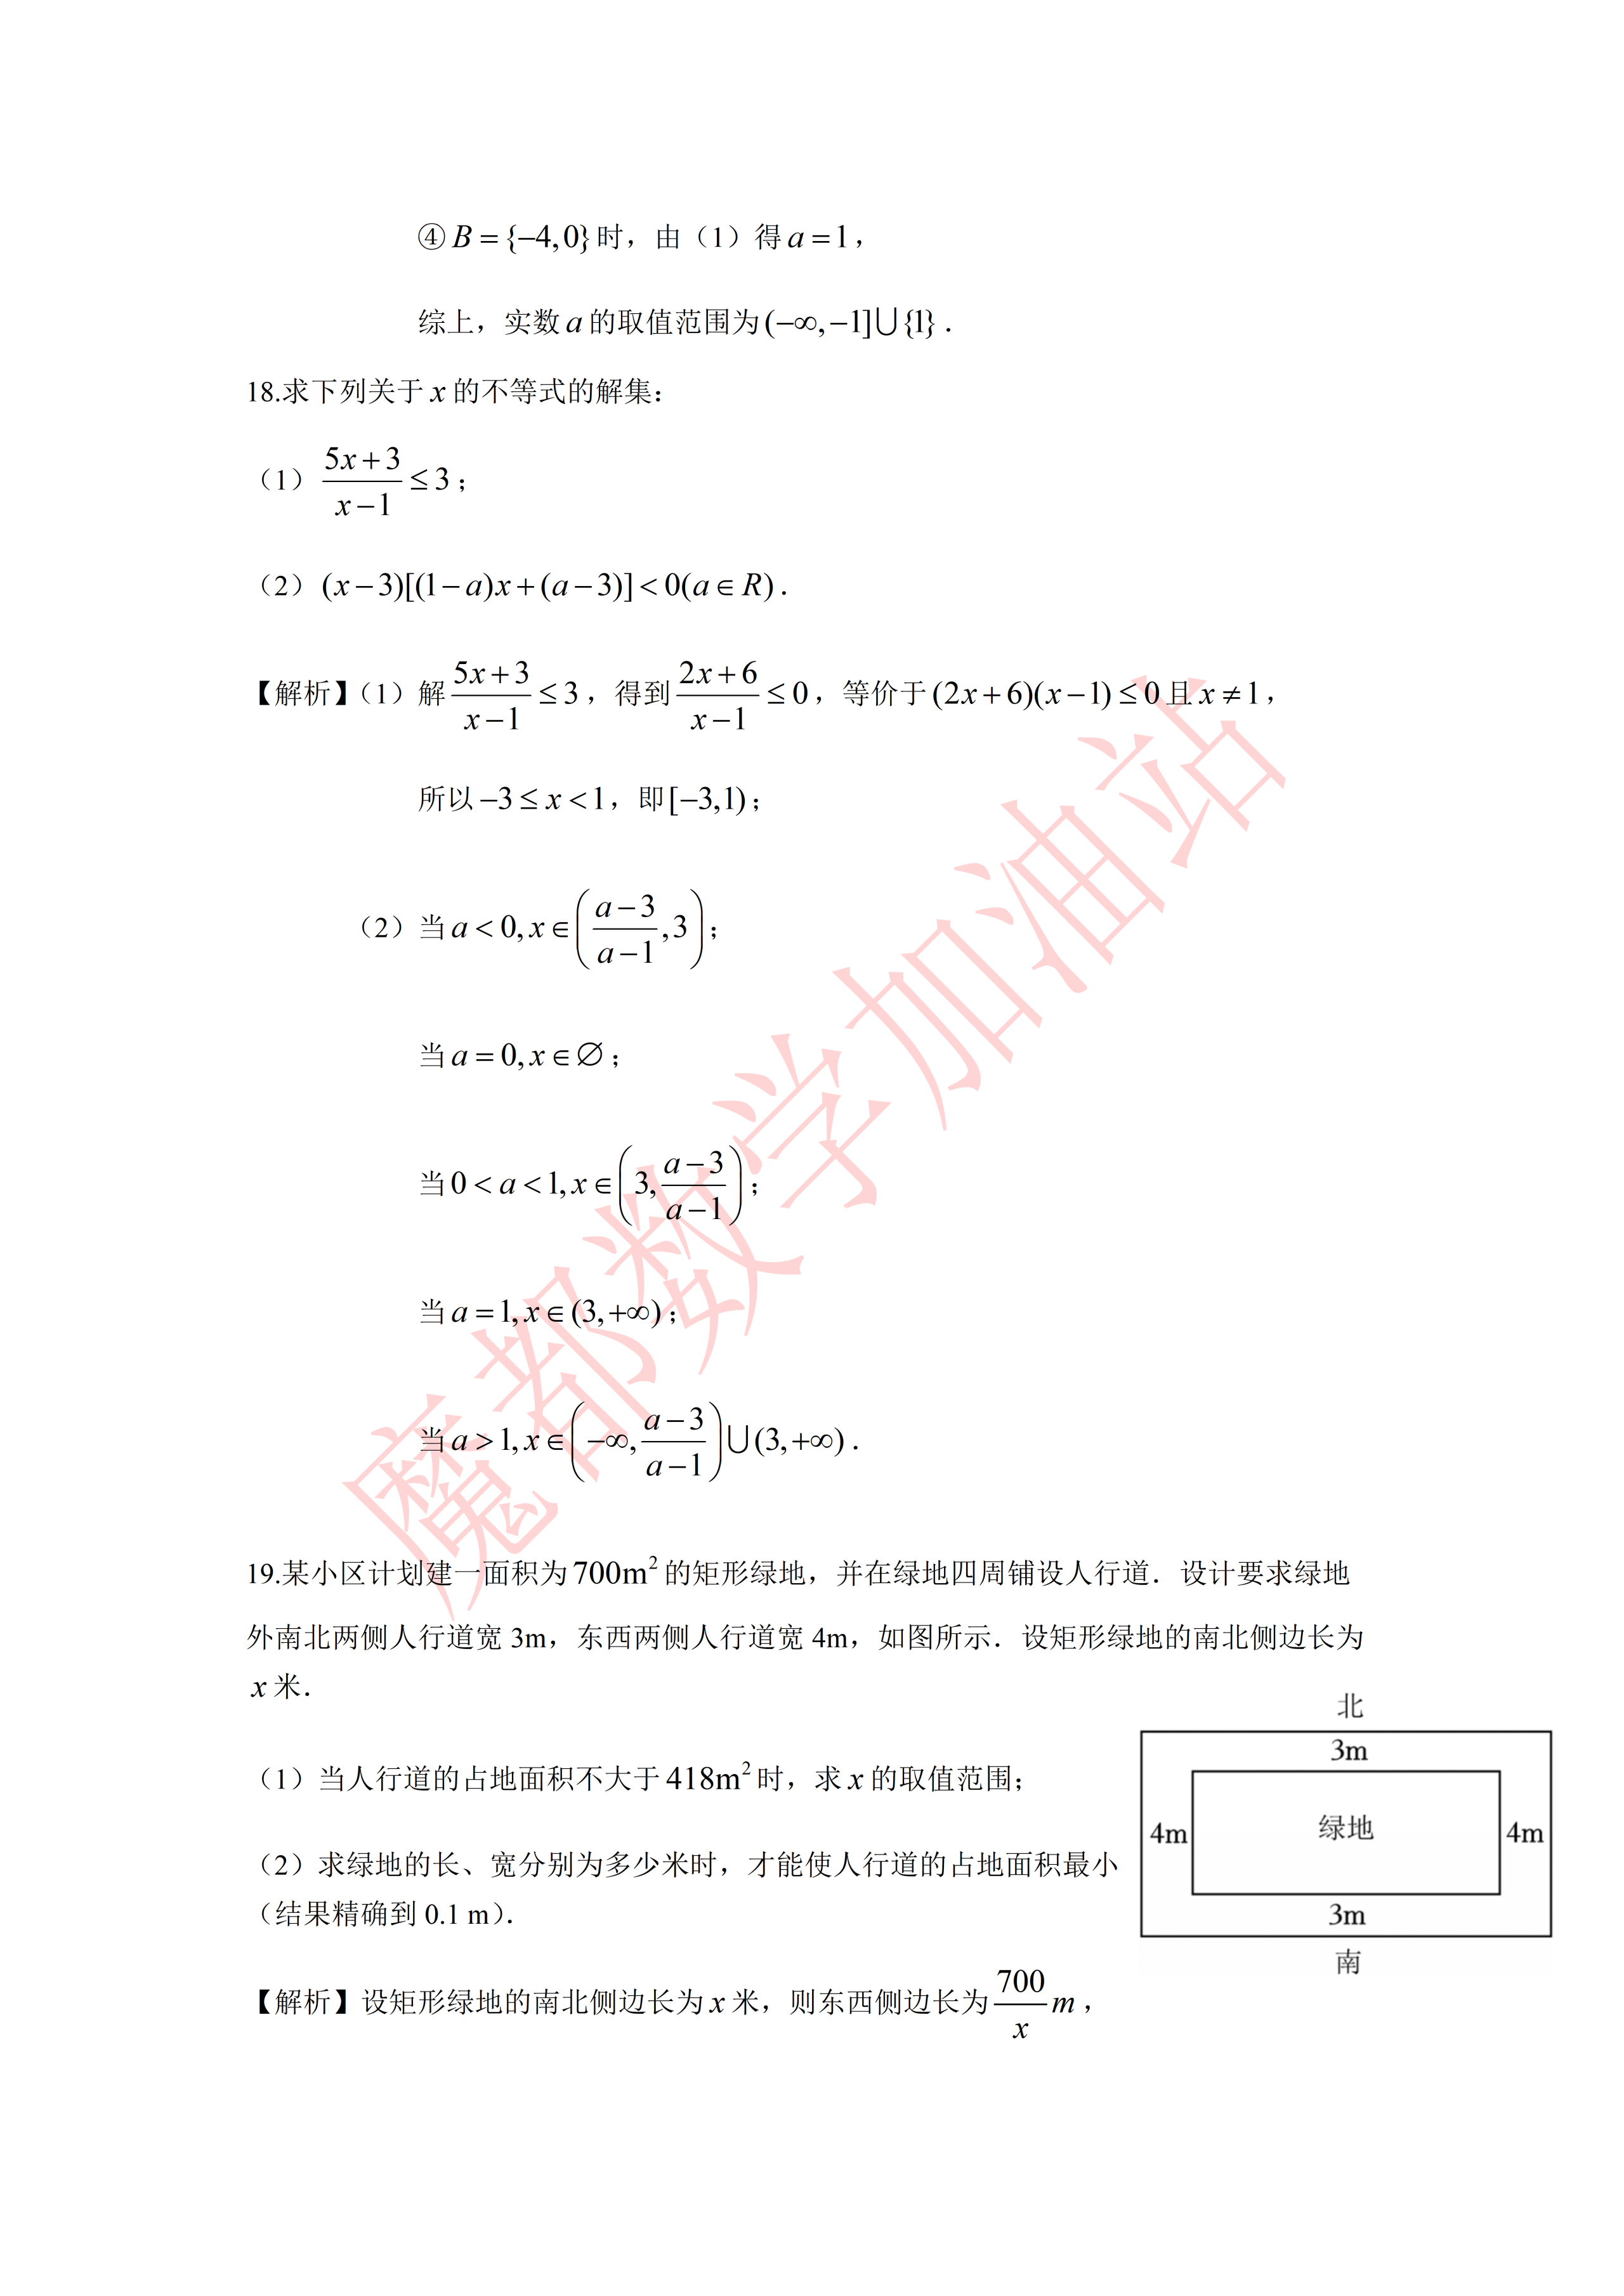
\includegraphics[width=.3\linewidth,trim=1791bp 484bp 107bp 2654bp,clip]{../原图/高一53_华师大二附中_10月月考/07.png}
\end{center}

\begin{enumerate}[label=(\arabic*)]
\item 当人行道的占地面积不大于 $418m^2$ 时，求 $x$ 的取值范围；
\item 求绿地的长、宽分别为多少米时，才能使人行道的占地面积最小（结果精确到 $0.1m$）.
\end{enumerate}

\ifanswer
\solbegin
\step{设矩形绿地的南北侧边长为 $x$ 米，则东西侧边长为 $\dfrac{700}{x}m$，}
\step{则人行道的占地面积为 $S=(x+8)\left(\dfrac{700}{x}+6\right)-700$，即 $S=6x+\dfrac{5600}{x}+48$.}
\stepm{(1)}{当人行道的占地面积不大于 $418m^2$ 时，$6x+\dfrac{5600}{x}+48\leqslant418$，}
\step{即 $6x^2-370x+5600\leqslant0$，解得 $\dfrac{80}{3}\leqslant x\leqslant35$，}
\step{故当人行道的占地面积不大于 $418m^2$ 时，$x\in\left[\dfrac{80}{3},35\right]$；}
\stepm{(2)}{$S=6x+\dfrac{5600}{x}+48\geqslant2\sqrt{6x\cdot\dfrac{5600}{x}}+48=80\sqrt{21}+48$，}
\step{当且仅当 $6x=\dfrac{5600}{x}$，即 $x=20\sqrt{\dfrac73}\approx30.6(m)$ 时，}
% 原卷如此，照录未改（80√21+48≈414.6，两处“414.4”疑笔误，见文件头“原卷笔误/存疑”第 6 条）
\step{$S$ 达到最小值 $80\sqrt{21}+48\approx414.4$，此时 $\dfrac{700}{x}\approx22.9(m)$，}
\step{所以当设计绿地的南北侧边长约为 $30.6m$，东西侧边长约为 $22.9m$ 时，}
\step{人行道的占地面积最小值为 $414.4(m^2)$.}
\solend
\fi

\ansspace[6]

\item 已知 $x\in\R$，符号 $[x]$ 表示不大于 $x$ 的最大整数，例如：$[2.3]=2$,$[2]=2$，$[-1.2]=-2$，令 $S(x)=[x]-[-x]$.

\begin{enumerate}[label=(\arabic*)]
\item 写出 $S(x)$ 为偶数（包括正、负偶数和 0）的充要条件，并证明；
\item 设方程 $|S(x)|=3$ 的解集为 $A$.

①集合 $B=\{x\mid x^2-ax-9\leqslant0,a\in\R\}$，若 $A\cap B=A$，求实数 $a$ 的取值范围；

②集合 $C=\{x\mid 2x^2-5kx+3k^2\geqslant0\}$，若 $A\cup C=\R$，求实数 $k$ 的取值范围.
\end{enumerate}

\ifanswer
\solbegin
\stepm{(1)}{$S(x)$ 为偶数的充要条件是 $x\in\Z$.}
\step{若 $x\in\Z$，则 $S(x)=[x]-[-x]=x-(-x)=2x$；}
\step{若 $x\notin\Z$，设 $[x]=n$，}
\step{则 $S(x)=[x]-[-x]=n-(-n-1)=2n+1=2[x]+1$；}
% 原卷如此，照录未改（“由①”按文意应为“由(1)”，见文件头“原卷笔误/存疑”第 3 条）
\stepm{(2)}{由①得 3 是奇数，$S(x)=\pm3$,$x\notin\Z$，}
\step{$S(x)=2[x]+1=\pm3$,$[x]=1$ 或 $-2$ 且 $x\notin\Z$，}
\step{所以 $A=(-2,-1)\cup(1,2)$；}
\stepm{①}{$A\cap B=A\Rightarrow A\subseteq B$，}
\step{设 $B=[x_1,x_2]$，其中 $x_1,x_2$ 是方程 $x^2-ax-9=0$ 的两实根，}
\step{设 $f(x)=x^2-ax-9$，}
\step{$[-2,2]\subseteq[x_1,x_2]\Leftrightarrow x_1\leqslant-2$,$x_2\geqslant2\Leftrightarrow\begin{cases}f(-2)\leqslant0\\ f(2)\leqslant0\end{cases}$}
\step{$\Leftrightarrow\begin{cases}(-2)^2-a\cdot(-2)-9\leqslant0, & a\leqslant\dfrac52\\ 2^2-2a-9\leqslant0, & a\geqslant-\dfrac52\end{cases}$，故 $a\in\left[-\dfrac52,\dfrac52\right]$；}
\step{注：若用求根公式 $\begin{cases}\dfrac{a+\sqrt{a^2+36}}{2}\geqslant2\Rightarrow a\geqslant-\dfrac52\\ \dfrac{a-\sqrt{a^2+36}}{2}\leqslant-2\Rightarrow a\leqslant\dfrac52\end{cases}$，结果正确，也得满分；}
\stepm{②}{$2x^2-5kx+3k^2=(x-k)(2x-3k)$.}
\step{$A\cup C=\R\Leftrightarrow\complement_\R A\subseteq C$.}
\step{记 $g(x)=2x^2-5kx+3k^2$，则 $\{x\mid g(x)<0\}\subseteq A$.}
\stepm{情况1：}{$k>0$ 时，$k<\dfrac32k$,$g(x)<0$ 的解集为 $\left(k,\dfrac32k\right)\subseteq(1,2)$，}
\step{故 $\begin{cases}k\geqslant1\\ \dfrac32k\leqslant2\end{cases}\Rightarrow1\leqslant k\leqslant\dfrac43$；}
\stepm{情况2：}{$k=0$ 时，$g(x)=2x^2\geqslant0$ 恒成立，$C=\R$,$A\cup C=\R$ 显然成立；}
\stepm{情况3：}{$k<0$ 时，$\dfrac32k<k$,$g(x)<0$ 的解集为 $\left(\dfrac32k,k\right)\subseteq(-2,-1)$，}
\step{故 $\begin{cases}\dfrac32k\geqslant-2\\ k\leqslant-1\end{cases}\Rightarrow-\dfrac43\leqslant k\leqslant-1$；}
\step{综上，$k\in\left[-\dfrac43,-1\right]\cup\{0\}\cup\left[1,\dfrac43\right]$.}
\solend
\fi

\ansspace[10]

\item 对于非空实数集 $M\subseteq(0,+\infty)$，若满足以下两个条件，则称 $M$ 为“极闭集”：

①$M$ 中至少含有 2 个元素，且 $1\notin M$；

②对于 $M$ 中任意两个不相等的元素 $x,y$，定义 $x*y=\dfrac{xy+1}{x+y}$，且 $x*y\in M$.

\begin{enumerate}[label=(\arabic*)]
\item 判断集合 $A=\left\{\dfrac12,2\right\}$ 与区间 $B=(1,+\infty)$ 是否为“极闭集”，并说明理由；
\item 若 $M$ 是“极闭集”，证明：集合 $M$ 中不可能所有元素都小于 1；
\item 证明：不存在任何有限的“极闭集”.
\end{enumerate}

\ifanswer
\solbegin
% 原卷如此，照录未改（首行集合按题干应为 {1/2,2}，见文件头“原卷笔误/存疑”第 7 条）
\stepm{(1)}{对于集合 $A=\left\{\dfrac12,1\right\}$，$\dfrac12*2=\dfrac45$，}
\step{因为 $\dfrac45\notin A$，不满足条件②，所以集合 $A$ 不是“极闭集”.}
\step{对于区间 $B$，满足条件①.}
\step{任取 $B$ 中两个不相等的元素 $x,y$，则 $x>1$,$y>1$.}
\step{$x*y-1=\dfrac{xy+1}{x+y}-1=\dfrac{(x-1)(y-1)}{x+y}>0$，所以 $x*y>1$，}
\step{这说明 $x*y\in B$ 恒成立，满足条件②，所以 $B$ 是“极闭集”.}
\stepm{(2)}{假设集合 $M$ 中所有元素都小于 1，}
\step{在 $M$ 中取 $0<x<y<1$,$x*y-1=\dfrac{xy+1}{x+y}-1=\dfrac{(x-1)(y-1)}{x+y}>0$，}
\step{所以 $x*y>1$，与“集合 $M$ 中所有元素都小于 1”矛盾，}
\step{假设不成立，集合 $M$ 中不可能所有元素都小于 1，得证.}
\stepm{(3)}{由②得，任何一个“极闭集”$M$ 中，必然至少存在一个大于 1 的元素，}
\stepm{情况1：}{若 $M$ 中至少存在两个大于 1 的元素，}
\step{设其中两个不相等的元素为 $x$ 和 $y_1$，且 $x>y_1>1$，}
\step{令 $y_{n+1}=x*y_n$,$n\geqslant1$,$y_{n+1}-1=x*y_n-1=\dfrac{(x-1)(y_n-1)}{xy_n+1}>0$，}
\step{如果 $y_n\geqslant1$，则显然 $y_{n+1}\geqslant1$，作差 $y_n-y_{n+1}=\dfrac{y_n^2-1}{x+y_n}>0$，}
\step{由此 $x>y_1>y_2>y_3>\cdots>1$，与有限集矛盾.}
\stepm{情况2：}{若 $M$ 中恰好只有一个元素大于 1，}
\step{设这个唯一大于 1 的元素为 $m$.}
\step{因为 $M$ 至少有两个元素，所以 $M$ 中必然至少存在一个元素 $a_1<1$，}
\step{令 $a_{n+1}=m*a_n$,$n\geqslant1$，}
\step{又 $a_{n+1}-1=m*a_n-1=\dfrac{(m-1)(a_n-1)}{m+a_n}<0$，故 $a_{n+1}<1$，}
\step{作差 $a_{n+1}-a_n=\dfrac{1-a_n^2}{m+a_n}>0$，由此 $a_1<a_2<a_3<\cdots<1$，与有限集矛盾.}
\step{因此，不存在任何有限的“极闭集”. 原命题得证.}
\solend
\fi

\ansspace*[10]

\end{enumerate}

\end{document}
"
%
% 原始材料：微信公众号“魔都数学加油站”文章，作者破晓，连载“27学年高一53”；
% 原文标题“27学年高一53——2026-2027年上海市华师大二附中高一上10月月考”；
% 原文链接：https://mp.weixin.qq.com/s/fpSnoF-gJEEWyxAoPC_bZA。
% 页面标注发布时间 2026-10-09 17:15（上海）。
% 正文为 11 张 PNG 页：第 01—06、08、10 页 4762×6735，第 07、09、11 页 2560×3620
% （**同一篇各页分辨率不同**），均按页序读取。11 页全为试卷正文页（卷首标题在第 1 页页顶，
% 卷末解答题第 21 题解析止于第 11 页），无封面页、目录页、二维码或宣传页。
% 粉色斜排“魔都数学加油站”为卷面水印，与公众号页脚一并未录入。
%
% 卷首标题：照卷面印作“2026--2027 年华师大二附中高一上 10 月月考”（公众号标题中的“上海市”
% 卷面标题行没有，本稿照卷面），年份区间按全稿惯例排 en dash。原卷只有一行标题、无副标题。
%
% 篇幅与题号：原卷自第 3 题起编号（第 1、2 题不在本卷内）。填空题 3—12（10 题）、
% 选择题 13—16（4 题）、解答题 17—21（5 题），共 19 题。本稿沿用原节与原题号，
% 只改排为全稿统一的大节样式（原卷小节标题为“一、填空题”“二、选择题”“三、解答题”）。
%
% 讲评版：原卷每题下直接印【答案】或【解析】。**第 13 题没有任何【答案】/【解析】段**，
% 答案“C”直接印在题干括号内（“一定不是(  C  )”），本稿按 高一37 第 13 题的成例把括号留空、
% 答案另提为 \ans{$C$}；其余 18 题都只印【解析】，按全稿口径这类题不另提 \ans{}——其中
% 选择题第 14、15、16 题的结论写在解析末句（“故选 B／D／C”），亦照录在解析内。
%
% 副标题：原卷未印副标题。本稿按“知识模块”口径标作“集合与常用逻辑用语、不等式”：
% 19 题中集合与常用逻辑用语 12 题（集合类 9 题——第 4、5、12、13、15、16、17、20、21 题；
% 逻辑类 3 题——第 3、9、14 题），不等式 7 题（含一元二次方程与绝对值方程：第 6、7、8、10、
% 11、18、19 题，其中第 11 题实为奇偶分析下的集合计数题，暂挂不等式），两类均超三分之一，
% 故并标。口径同 高一46、高一47、高一48、高一51、高一52。
%
% 与原卷的排版差异：
%   ① 原卷每题下直接印【解析】，本稿按全稿惯例将答案与解析置于答案版，试卷版保持干净；
%      第 13 题印在题干括号内的答案“C”同样移入 \ans{}，见上；
%   ② 原卷未印副标题，本稿按“知识模块”口径补出；
%   ③ 原卷填空横线约两个字宽，本稿按全稿惯例统一排 \blankline[4.4em]；
%      选择题的作答括号原卷排半角“(    )”，本稿按全稿惯例排 \mbox{（\quad）}；
%   ④ 原卷实数集排斜体/粗体 $R$、$\mathbf{R}$（第 4、6、7、18、20 题等处），本稿按全稿惯例
%      改用 $\R$；空集记号统一为 \varnothing；
%   ⑤ 原卷在数学式内多处用半角逗号（如 $x_1,x_2$、$|S|,|T|$、$a\neq0,c\neq0$），均照录未强改；
%      句末句点按全稿惯例排西文句点（原卷“故选 B．”一类全角句点亦从宽排作“.”）；
%   ⑥ 第 17—21 题的子问原卷各自另起一行，本稿按全稿惯例用 enumerate 的 (1)(2)(3)；
%      第 20 题 (2) 问下的①②两行是题干的一部分，照录为行首①②标号（不入 enumerate）；
%      解析中的子问标号一律用 \stepm{(1)}{…}，解析中的①②③④分情形用 \stepm{①}{…}；
%   ⑦ 第 12、20、21 题解析里的“情况1:”至“情况3:”标号原卷排**红色加粗**（全卷共 6 处），
%      全库无红色排字先例，本稿按全稿子题标号样式排 \stepm{情况1：}{…}（加粗着色、不改黑色基调），
%      冒号照原卷排全角；
%   ⑧ 第 19 题的示意图原卷排在题干右侧（与题干、(1) 问同高），本稿居中排在题干之后、
%      子问之前，并在 \item 前加 \needvspace 整块推走；图自原图第 07 页裁切（trim），不另存图片文件；
%   ⑨ 每道解答题原卷未留作答空白，本稿按全稿惯例加 \ansspace。
%
% 原卷笔误/存疑（均照录未改，正文对应处另有 % 注）：
%   1. 第 14 题解析末行“例如 $a=1$，$b=-1$，及必要性不成立”，“及”按文意应为“即”；
%   2. 第 15 题解析第 3 行 $\dfrac1{a+b\sqrt2}=\dfrac a{a^2-2b}+\left(-\dfrac b{a^2-2b}\right)\cdot\sqrt2$，
%      分母两处均作 $a^2-2b$，按通分应为 $a^2-2b^2$（结论 $C=X$ 不受影响）；
%   3. 第 20 题 (2) 问解析首行“由①得 3 是奇数”，按文意应为“由(1)得”（①是 (2) 问下自己
%      的子问标号，奇偶性结论出自 (1) 问）；
%   4. 第 11 题解析“只有奇数的有 $C_4^2+1=7$ 个”，按组合意义应为 $C_4^2+C_4^4=7$
%      （“$+1$”当指 4 个奇数全取的 1 种），数值无误；
%   5. 第 18 题 (2) 问解析“当 $a=0$,$x\in\varnothing$”，按文意应为“解集为 $\varnothing$”；
%   6. 第 19 题 (2) 问解析“$S$ 达到最小值 $80\sqrt{21}+48\approx414.4$”与末行
%      “人行道的占地面积最小值为 $414.4(m^2)$”，两处按 $80\sqrt{21}+48\approx414.6$，疑笔误；
%   7. 第 21 题 (1) 问解析首行“对于集合 $A=\left\{\frac12,1\right\}$”，按题干应为
%      $A=\left\{\frac12,2\right\}$（计算 $\frac12*2=\frac45$ 用的正是 $2$）；
%   8. 第 12 题解析“所以 $A=(-\infty,-4]\cup[2,+\infty)$”一行行末无标点，体例不一，照录。
%
% 插图：1 张，自原图裁切（无 \begin{tikzpicture} 重排）：
%   · 第 19 题绿地示意图（外矩形内套矩形“绿地”，上“北 3m”、下“南 3m”、左右各“4m”）
%     ——原图第 07 页，原卷排于题干右侧。
%     裁框：x 1797–2447、y 2660–3136（含“北”“南”标注，四周各留约 6px），
%     trim=1791bp 484bp 107bp 2654bp（左／下／右／上），页宽 2560、页高 3620。
%
\documentclass[a4paper,11pt]{article}
\usepackage{common}

\begin{document}

\examtitlest[3]{2026--2027 年华师大二附中高一上 10 月月考}{集合与常用逻辑用语、不等式}

\bigsec{一、填空题}

\begin{enumerate}
\setcounter{enumi}{2}

\item “$x=2$”是“$x^2-3x+2=0$”的\blankline[4.4em]条件.

（选择其中之一填空：充分非必要、必要非充分、充分、既非充分又非必要）

\ifanswer
\solbegin
\step{由 $x^2-3x+2=0$ 得 $x=1$ 或 $x=2$，}
\step{则“$x=2$”是“$x^2-3x+2=0$”的充分不必要条件.}
\solend
\fi

\item 已知 $R$ 是全集，集合 $A=\{y\mid y=-x^2+1,x\in\R\}$，集合 $B=\{x\mid x=3+|a|,a\in\R\}$，则 $\overline{A\cup B}=$\blankline[4.4em].

\ifanswer
\solbegin
\step{$A=\{y\mid y=-x^2+1,x\in\R\}=(-\infty,1]$，$B=\{x\mid x=3+|a|,a\in\R\}=[3,+\infty)$，}
\step{所以 $\overline{A\cup B}=(1,3)$.}
\solend
\fi

\item 已知 $a$ 为常数，集合 $A=\{x\mid x^2+x-6=0\}$，集合 $B=\{x\mid ax-2=0\}$，且 $B\subseteq A$，则 $a$ 的所有取值构成的集合为\blankline[4.4em].

\ifanswer
\solbegin
\step{集合 $A=\{-3,2\}$，因为 $B\subseteq A$，则 $B=\varnothing$，$\{-3\}$，$\{2\}$，$\{-3,2\}$，}
\step{当 $B=\varnothing$ 时，$a=0$，当 $B=\{-3\}$ 时，$a=-\dfrac23$，当 $B=\{2\}$ 时，$a=1$，}
\step{当 $B=\{-3,2\}$ 时，不成立，故 $a$ 的取值集合为 $\left\{0,-\dfrac23,1\right\}$.}
\solend
\fi

\item 设 $a\in\R$，若关于 $x$ 的不等式 $x^2-ax<0$ 的解集是区间 $(0,1)$ 的真子集，则 $a$ 的取值范围是\blankline[4.4em].

\ifanswer
\solbegin
\step{因为关于 $x$ 的不等式 $x^2-ax<0$ 的解集是区间 $(0,1)$ 的真子集，}
\step{当 $a=0$ 时，不等式的解集为 $\varnothing$，符合题意；}
\step{当 $a>0$ 时，不等式的解集为 $(0,a)$，则 $0<a<1$，}
\step{当 $a<0$ 时，不等式的解集为 $(a,0)$，不符合题意，}
\step{故 $a$ 的范围为 $[0,1)$.}
\solend
\fi

\item 设 $x\in\R$，则方程 $|2x+3|-|x-2|=|3x+1|$ 的解集为\blankline[4.4em].

\ifanswer
\solbegin
\step{当 $x\leqslant-\dfrac32$ 时，原式$\Leftrightarrow-2x-3+x-2=-3x-1\Leftrightarrow x=2$，不合题意；}
\step{当 $-\dfrac32<x\leqslant-\dfrac13$ 时，原式$\Leftrightarrow2x+3+x-2=-3x-1\Leftrightarrow x=-\dfrac13$；}
\step{当 $-\dfrac13<x\leqslant2$ 时，原式$\Leftrightarrow2x+3+x-2=3x+1\Leftrightarrow1=1$ 即恒成立；}
\step{当 $x>2$ 时，原式$\Leftrightarrow2x+3+2-x=3x+1\Leftrightarrow x=2$，不合题意；}
\step{故 $x\in\left[-\dfrac13,2\right]$.}
\solend
\fi

\item 已知关于 $x$ 的一元二次方程 $x^2+(4m+1)x+2m-1=0$．若方程的两根为 $x_1$、$x_2$，且满足 $\dfrac1{x_1}+\dfrac1{x_2}=-\dfrac12$，则实数 $m=$\blankline[4.4em].

\ifanswer
\solbegin
\step{由于判别式$\Delta=16m^2+5>0$恒成立，}
\step{不论 $m$ 为任何实数，方程总有两个不相等的实数根.}
\step{$\dfrac1{x_1}+\dfrac1{x_2}=-\dfrac12$，即 $\dfrac{x_1+x_2}{x_1x_2}=-\dfrac12$，由根与系数的关系得 $\dfrac{-4m-1}{2m-1}=-\dfrac12$，}
\step{解得 $m=-\dfrac12$.}
\solend
\fi

\item 已知 $\dfrac1{x-2}\geqslant1$ 是 $|x-a|<2$ 的充分非必要条件，则实数 $a$ 的取值范围是\blankline[4.4em].

\ifanswer
\solbegin
\step{由 $\dfrac1{x-2}\geqslant1$ 得 $\dfrac{3-x}{x-2}\geqslant0$，解得 $2<x\leqslant3$，由 $|x-a|<2$ 得 $a-2<x<a+2$，}
\step{因为 $\dfrac1{x-2}\geqslant1$ 是 $|x-a|<2$ 的充分非必要条件，}
\step{所以 $\{x\mid 2<x\leqslant3\}\subset\{x\mid a-2<x<a+2\}$，所以 $\begin{cases}a-2\leqslant2\\ a+2>3\end{cases}$，解得 $1<a\leqslant4$，}
\step{即实数 $a$ 的取值范围是 $(1,4]$.}
\solend
\fi

\item 设 $x,y\in(0,+\infty)$，且 $x+4y=1$，则 $\dfrac1x+\dfrac1y$ 的最小值为\blankline[4.4em].

\ifanswer
\solbegin
\step{因为 $\dfrac1x+\dfrac1y=(x+4y)\left(\dfrac1x+\dfrac1y\right)=5+\dfrac{4y}{x}+\dfrac{x}{y}\geqslant5+2\sqrt{\dfrac{4y}{x}\cdot\dfrac{x}{y}}=9$，}
\step{当且仅当 $\dfrac{4y}{x}=\dfrac{x}{y}$，即 $x=2y$，即 $x=\dfrac13$,$y=\dfrac16$ 时取等号，故最小值为 $9$.}
\solend
\fi

\item 设非空集合 $Q\subseteq M$，当 $Q$ 中所有元素和为偶数时（集合为单元素时和为元素本身），称 $Q$ 是 $M$ 的偶子集. 若集合 $M=\{1,2,3,4,5,6,7\}$，则其偶子集 $Q$ 的个数为\blankline[4.4em].

\ifanswer
\solbegin
\step{偶子集可以分为只有奇数、偶数及偶数个奇数和偶数的集合，}
\step{奇数有 4 个，偶数有 3 个，}
% 原卷如此，照录未改：按组合意义应为 C_4^2+C_4^4=7（“+1”当指 4 个奇数全取的 1 种），
% 见文件头“原卷笔误/存疑”第 4 条
\step{只有奇数的有 $C_4^2+1=7$ 个，只有偶数的有 $C_3^1+C_3^2+1=7$ 个，}
\step{偶数个奇数和偶数的：两奇一偶 $C_4^2\cdot C_3^1=18$ 个，两奇二偶 $C_4^2\cdot C_3^2=18$ 个，}
\step{两奇三偶 $C_4^2\cdot C_3^3=6$ 个，四奇一偶 $C_4^4\cdot C_3^1=3$ 个，四奇二偶 $C_4^4\cdot C_3^2=3$ 个，}
\step{四奇三偶 $C_4^4\cdot C_3^3=1$ 个，所以共有 $7+7+18+18+6+3+3+1=63$ 个.}
\solend
\fi

\item 已知集合 $A=\{x\mid x^2+2x-8\geqslant0\}$,$B=\{x\mid x^2-2ax+2a\leqslant0\}$，且 $A\cap B$ 中恰有 3 个整数元素，则实数 $a$ 的取值范围为\blankline[4.4em].

\ifanswer
\solbegin
% 原卷如此，照录未改：此行行末无标点，见文件头“原卷笔误/存疑”第 8 条
\step{由 $x^2+2x-8\geqslant0$，得 $x\geqslant2$ 或 $x\leqslant-4$，所以 $A=(-\infty,-4]\cup[2,+\infty)$}
\step{对集合 $B$：$x^2-2ax+2a\leqslant0$,$\Delta=4a^2-8a=4a(a-2)\geqslant0$，}
\step{得 $a\leqslant0$ 或 $a\geqslant2$.}
\step{设方程 $x^2-2ax+2a=0$ 的两根为 $r_1,r_2$，}
\step{则 $B=[r_1,r_2]$,$r_1=a-\sqrt{a^2-2a}$,$r_2=a+\sqrt{a^2-2a}$，}
\stepm{情况1：}{$a\leqslant0$，}
\step{$r_2=a+\sqrt{a^2-2a}<a+\sqrt{a^2-2a+1}=a+|a-1|=a+1-a=1<2$，}
\step{$B$ 只在 $A$ 的左侧部分有交集，要使 $A\cap B$ 恰有 3 个整数元素，}
\step{这 3 个整数为 $-6,-5,-4$，于是 $r_1\in(-7,-6]$，}
\step{令 $f(x)=x^2-2ax+2a$，则 $\begin{cases}f(-7)=49+14a+2a>0\\ f(-6)=36+12a+2a\leqslant0\end{cases}\Rightarrow a\in\left(-\dfrac{49}{16},-\dfrac{18}{7}\right]$；}
\stepm{情况2：}{$a\geqslant2$，}
\step{$r_2=a+\sqrt{a^2-2a}\geqslant2$，}
\step{$r_1=a-\sqrt{a^2-2a}>a-\sqrt{a^2-2a+1}=a-|a-1|=a-(a-1)=1>-4$，}
\step{所以 $A\cap B=[2,r_2]$.}
\step{同理 $\begin{cases}f(4)=16-8a+2a\leqslant0\\ f(5)=25-10a+2a>0\end{cases}\Rightarrow a\in\left[\dfrac{8}{3},\dfrac{25}{8}\right)$；}
\step{综上，$a\in\left(-\dfrac{49}{16},-\dfrac{18}{7}\right]\cup\left[\dfrac{8}{3},\dfrac{25}{8}\right)$.}
\solend
\fi

\end{enumerate}

\bigsec{二、选择题}

\begin{enumerate}
\setcounter{enumi}{12}

% 第 13 题原卷无【答案】/【解析】段，答案“C”直接印在题干括号内，
% 按高一37 第 13 题的成例括号留空、答案另提为 \ans{}（见文件头）
\item 集合 $A=\{a,b,c\}$ 中的三个元素分别表示某一个三角形的三边长度，那么这个三角形一定不是\mbox{（\quad）}

\keepwithprev
A. 锐角三角形\qquad B. 钝角三角形

C. 等腰三角形\qquad D. 直角三角形

\ifanswer
\ans{$C$}
\fi

\item 设 $a$、$b$ 为实数，则“$a<b<0$”是“$\dfrac1a>\dfrac1b$”的\mbox{（\quad）}条件.

\keepwithprev
A. 充要\qquad B. 充分不必要

C. 必要不充分\qquad D. 既不充分也不必要

\ifanswer
\solbegin
\step{若 $a<b<0$，则 $\dfrac1a>\dfrac1b$ 一定成立，即充分性成立；}
% 原卷如此，照录未改（“及”按文意应为“即”，见文件头“原卷笔误/存疑”第 1 条）
\step{若 $\dfrac1a>\dfrac1b$ 成立，$a<b<0$ 不一定成立，例如 $a=1$，$b=-1$，及必要性不成立.}
\step{故选 $B$.}
\solend
\fi

\item 设 $Q$ 表示有理数集，集合 $X=\{x\mid x=a+b\sqrt2,a,b\in Q,x\neq0\}$，在下列集合中：①$\{2x\mid x\in X\}$②$\left\{\dfrac{x}{\sqrt2}\mid x\in X\right\}$③$\left\{\dfrac1x\mid x\in X\right\}$④$\{x^2\mid x\in X\}$，与 $X$ 相同的集合有\mbox{（\quad）}

\keepwithprev
A. ①②③④\qquad B. ②③④\qquad C. ①②④\qquad D. ①②③

\ifanswer
\solbegin
\step{$A=\{2x\mid x\in X\}$，$2(a+b\sqrt2)=p+q\sqrt2$ 得 $p=2a$，$q=2b$，$a=\dfrac p2$，$b=\dfrac q2$，}
\step{也是一一对应，$A=X$}
% 原卷如此，照录未改：分母两处均作 a^2-2b，按通分应为 a^2-2b^2，
% 见文件头“原卷笔误/存疑”第 2 条
\step{集合 $B=\left\{\dfrac{x}{\sqrt2}\mid x\in X\right\}$，$\dfrac{a+b\sqrt2}{\sqrt2}=b+\dfrac a2\cdot\sqrt2$，也是一一对应，$B=X$}
\step{集合 $C=\left\{\dfrac1x\mid x\in X\right\}$，$\dfrac{1}{a+b\sqrt2}=\dfrac{a}{a^2-2b}+\left(-\dfrac{b}{a^2-2b}\right)\cdot\sqrt2$，一一对应，$C=X$}
\step{集合 $D=\{x^2\mid x\in X\}$，$(a+b\sqrt2)^2=a^2+2b^2+2ab\sqrt2$，这个不能一一对应了，}
\step{集合 $D$ 包含于 $X$ 中.}
\step{故 $X$ 相同的集合有①②③，故选 $D$.}
\solend
\fi

\item 集合 $S=\{x\mid(x+a)(x^2+bx+c)=0\}$,$T=\{x\mid(ax+1)(cx^2+bx+1)=0\}$，其中 $a,b,c$ 为实数，若 $|S|,|T|$ 分别表示集合 $S,T$ 的元素个数，则 $|S|-|T|$ 的所有可能取值集合为\mbox{（\quad）}

\keepwithprev
A. $\{0\}$\qquad B. $\{1\}$\qquad C. $\{0,1\}$\qquad D. $\{-1,0,1\}$

\ifanswer
\solbegin
\stepm{①}{$a\neq0,c\neq0$ 时.}
\step{$S$ 中 $x+a=0$ 的根 $x=-a$;$T$ 中 $ax+1=0$ 的根 $x=-\dfrac1a$.}
\step{$S$ 中的 $x^2+bx+c=0$ 若无实根，则 $T$ 中的 $cx^2+bx+1=0$ 也无实根；}
\step{又设 $S$ 的 $x^2+bx+c=0$ 的根为 $r(r\neq0)$，则 $T$ 的 $cx^2+bx+1=0$ 的根为 $\dfrac1r$.}
\step{（因为 $r^2+br+c=0\Rightarrow c\cdot\left(\dfrac1r\right)^2+b\cdot\dfrac1r+1=0$）}
\step{即 $a\neq0,c\neq0$ 时，}
\step{$S$ 与 $T$ 的实根存在一一对应关系 $x\leftrightarrow\dfrac1x$,$|S|=|T|,$$|S|-|T|=0$；}
\stepm{②}{$a=0,c\neq0$ 时.}
\step{$S$ 中多出一个根 $x=0$，而 $T$ 中无此根，$|S|=|T|+1$，即 $|S|-|T|=1$；}
\stepm{③}{$a\neq0,c=0$ 时.}
\step{则 $S$ 中仍有根 $x=0$，而 $T$ 中无 0 根，同样 $|S|-|T|=1$.}
\stepm{④}{$a=0,c=0$ 时.}
\step{同样 $S$ 含有根 0，而 $T$ 中不含 0，仍有 $|S|-|T|=1$.}
\step{综上，$|S|-|T|$ 所有可能取值为 0 和 1，故选 $C$.}
\solend
\fi

\end{enumerate}

\bigsec{三、解答题}

\begin{enumerate}
\setcounter{enumi}{16}

\item 已知集合 $A=\{x\mid x^2+4x=0\}$，$B=\{x\mid x^2+2(a+1)x+a^2-1=0\}$.

\begin{enumerate}[label=(\arabic*)]
\item 若 $A$ 是 $B$ 的子集，求实数 $a$ 的值；
\item 若 $B$ 是 $A$ 的子集，求实数 $a$ 的取值范围.
\end{enumerate}

\ifanswer
\solbegin
\stepm{(1)}{因为 $A=\{-4,0\}$，$B=\{x\mid x^2+2(a+1)x+a^2-1=0\}$，又 $A\subseteq B$，}
\step{所以 $A=B$，所以 $\begin{cases}-4+0=-2(a+1)\\ -4\times0=a^2-1\end{cases}$，所以 $a=1$；}
\stepm{(2)}{因为 $B$ 是 $A$ 的子集，所以 $B=\varnothing$ 或 $B=\{-4\}$ 或 $B=\{0\}$ 或 $B=\{-4,0\}$，}
\stepm{①}{$B=\varnothing$ 时，$\Delta=4(a+1)^2-4(a^2-1)<0$，所以 $a<-1$；}
\stepm{②}{$B=\{-4\}$ 时，$\begin{cases}-4+(-4)=-2(a+1)\\ -4\times(-4)=a^2-1\end{cases}$，无解；}
\stepm{③}{$B=\{0\}$ 时，$\begin{cases}0+0=-2(a+1)\\ 0\times0=a^2-1\end{cases}$，所以 $a=-1$；}
\stepm{④}{$B=\{-4,0\}$ 时，由（1）得 $a=1$，}
\step{综上，实数 $a$ 的取值范围为 $(-\infty,-1]\cup\{1\}$.}
\solend
\fi

\ansspace[6]

\item 求下列关于 $x$ 的不等式的解集：

\begin{enumerate}[label=(\arabic*)]
\item $\dfrac{5x+3}{x-1}\leqslant3$；
\item $(x-3)[(1-a)x+(a-3)]<0$ ($a\in\R$).
\end{enumerate}

\ifanswer
\solbegin
\stepm{(1)}{解 $\dfrac{5x+3}{x-1}\leqslant3$，得到 $\dfrac{2x+6}{x-1}\leqslant0$，等价于 $(2x+6)(x-1)\leqslant0$ 且 $x\neq1$，}
\step{所以 $-3\leqslant x<1$，即 $[-3,1)$；}
\stepm{(2)}{当 $a<0$,$x\in\left(\dfrac{a-3}{a-1},3\right)$；}
% 原卷如此，照录未改（“x∈∅”按文意应为“解集为 ∅”，见文件头“原卷笔误/存疑”第 5 条）
\step{当 $a=0$,$x\in\varnothing$；}
\step{当 $0<a<1$,$x\in\left(3,\dfrac{a-3}{a-1}\right)$；}
\step{当 $a=1$,$x\in(3,+\infty)$；}
\step{当 $a>1$,$x\in\left(-\infty,\dfrac{a-3}{a-1}\right)\cup(3,+\infty)$.}
\solend
\fi

\ansspace[6]

\needvspace{13\baselineskip}

\item 某小区计划建一面积为 $700m^2$ 的矩形绿地，并在绿地四周铺设人行道. 设计要求绿地外南北两侧人行道宽 $3m$，东西两侧人行道宽 $4m$，如图所示. 设矩形绿地的南北侧边长为 $x$ 米.

\begin{center}
% 原图第 7 页题干绿地示意图直接裁取（原卷排于题干右侧）。
% 裁框取图形外框 x 1797–2447、y 2660–3136（含“北”“南”标注，四周各留约 6px），
% trim=左 1791bp／下 484bp／右 107bp／上 2654bp（页宽 2560、页高 3620）。
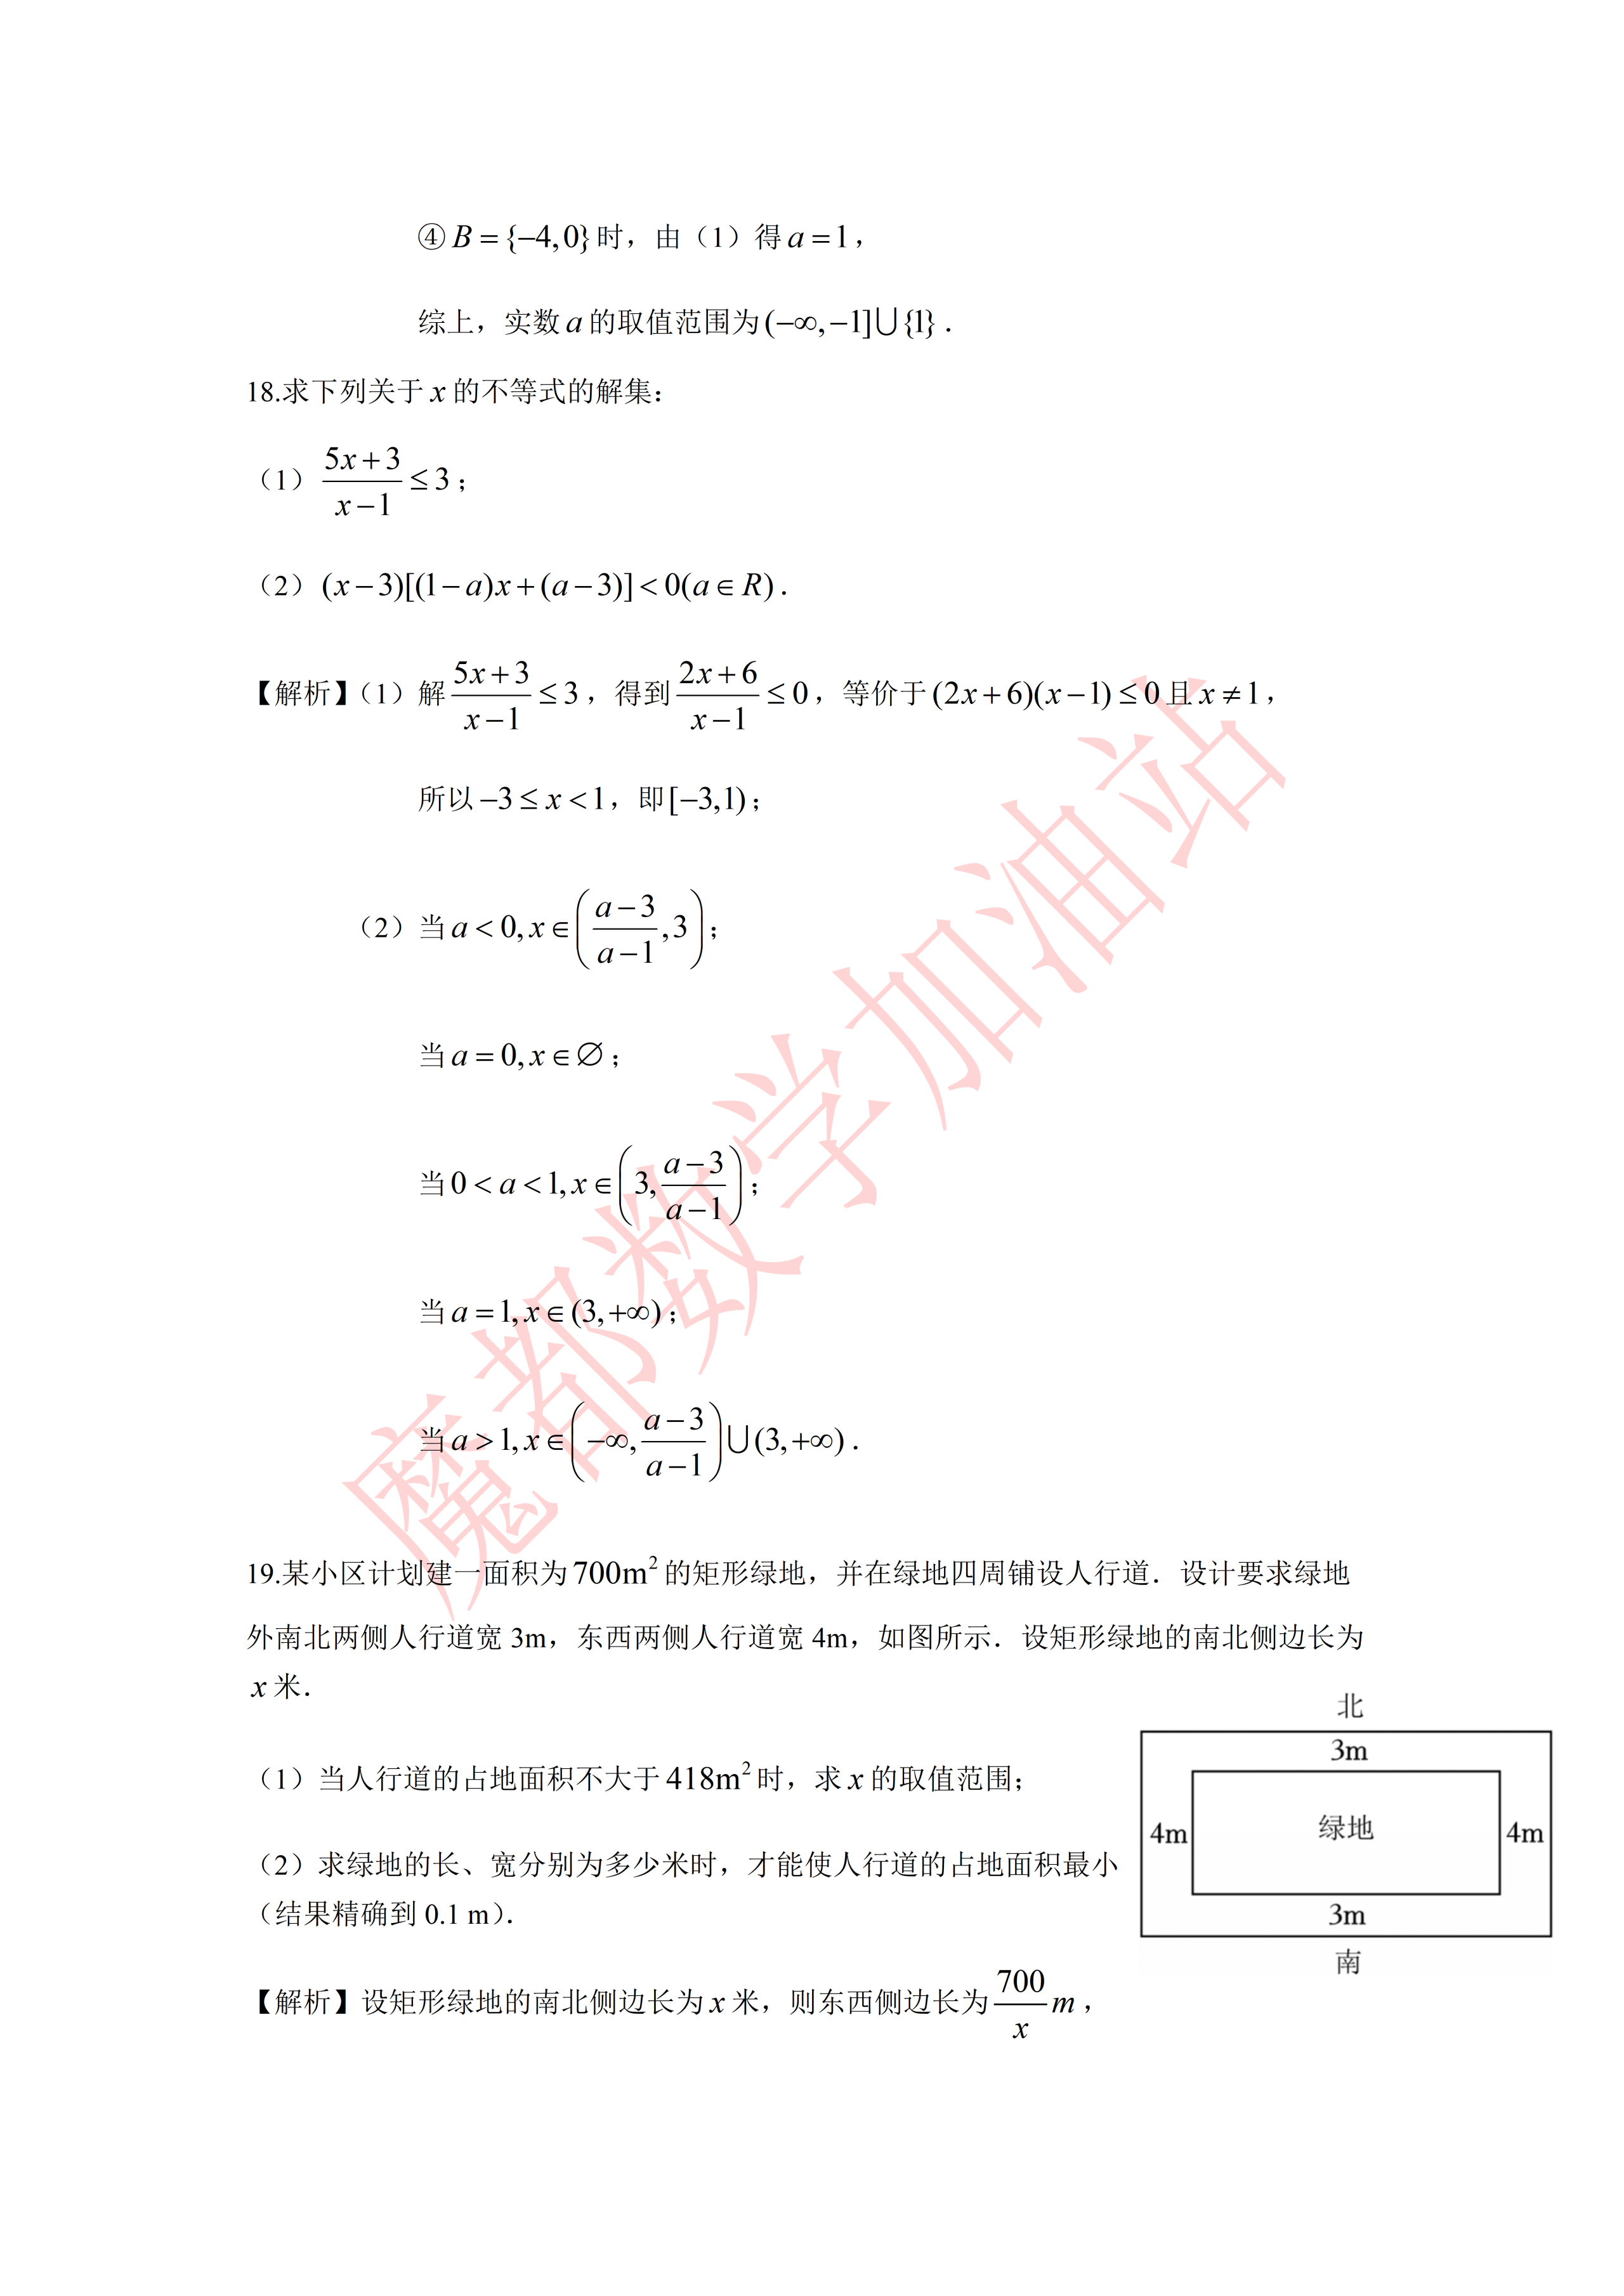
\includegraphics[width=.3\linewidth,trim=1791bp 484bp 107bp 2654bp,clip]{../原图/高一53_华师大二附中_10月月考/07.png}
\end{center}

\begin{enumerate}[label=(\arabic*)]
\item 当人行道的占地面积不大于 $418m^2$ 时，求 $x$ 的取值范围；
\item 求绿地的长、宽分别为多少米时，才能使人行道的占地面积最小（结果精确到 $0.1m$）.
\end{enumerate}

\ifanswer
\solbegin
\step{设矩形绿地的南北侧边长为 $x$ 米，则东西侧边长为 $\dfrac{700}{x}m$，}
\step{则人行道的占地面积为 $S=(x+8)\left(\dfrac{700}{x}+6\right)-700$，即 $S=6x+\dfrac{5600}{x}+48$.}
\stepm{(1)}{当人行道的占地面积不大于 $418m^2$ 时，$6x+\dfrac{5600}{x}+48\leqslant418$，}
\step{即 $6x^2-370x+5600\leqslant0$，解得 $\dfrac{80}{3}\leqslant x\leqslant35$，}
\step{故当人行道的占地面积不大于 $418m^2$ 时，$x\in\left[\dfrac{80}{3},35\right]$；}
\stepm{(2)}{$S=6x+\dfrac{5600}{x}+48\geqslant2\sqrt{6x\cdot\dfrac{5600}{x}}+48=80\sqrt{21}+48$，}
\step{当且仅当 $6x=\dfrac{5600}{x}$，即 $x=20\sqrt{\dfrac73}\approx30.6(m)$ 时，}
% 原卷如此，照录未改（80√21+48≈414.6，两处“414.4”疑笔误，见文件头“原卷笔误/存疑”第 6 条）
\step{$S$ 达到最小值 $80\sqrt{21}+48\approx414.4$，此时 $\dfrac{700}{x}\approx22.9(m)$，}
\step{所以当设计绿地的南北侧边长约为 $30.6m$，东西侧边长约为 $22.9m$ 时，}
\step{人行道的占地面积最小值为 $414.4(m^2)$.}
\solend
\fi

\ansspace[6]

\item 已知 $x\in\R$，符号 $[x]$ 表示不大于 $x$ 的最大整数，例如：$[2.3]=2$,$[2]=2$，$[-1.2]=-2$，令 $S(x)=[x]-[-x]$.

\begin{enumerate}[label=(\arabic*)]
\item 写出 $S(x)$ 为偶数（包括正、负偶数和 0）的充要条件，并证明；
\item 设方程 $|S(x)|=3$ 的解集为 $A$.

①集合 $B=\{x\mid x^2-ax-9\leqslant0,a\in\R\}$，若 $A\cap B=A$，求实数 $a$ 的取值范围；

②集合 $C=\{x\mid 2x^2-5kx+3k^2\geqslant0\}$，若 $A\cup C=\R$，求实数 $k$ 的取值范围.
\end{enumerate}

\ifanswer
\solbegin
\stepm{(1)}{$S(x)$ 为偶数的充要条件是 $x\in\Z$.}
\step{若 $x\in\Z$，则 $S(x)=[x]-[-x]=x-(-x)=2x$；}
\step{若 $x\notin\Z$，设 $[x]=n$，}
\step{则 $S(x)=[x]-[-x]=n-(-n-1)=2n+1=2[x]+1$；}
% 原卷如此，照录未改（“由①”按文意应为“由(1)”，见文件头“原卷笔误/存疑”第 3 条）
\stepm{(2)}{由①得 3 是奇数，$S(x)=\pm3$,$x\notin\Z$，}
\step{$S(x)=2[x]+1=\pm3$,$[x]=1$ 或 $-2$ 且 $x\notin\Z$，}
\step{所以 $A=(-2,-1)\cup(1,2)$；}
\stepm{①}{$A\cap B=A\Rightarrow A\subseteq B$，}
\step{设 $B=[x_1,x_2]$，其中 $x_1,x_2$ 是方程 $x^2-ax-9=0$ 的两实根，}
\step{设 $f(x)=x^2-ax-9$，}
\step{$[-2,2]\subseteq[x_1,x_2]\Leftrightarrow x_1\leqslant-2$,$x_2\geqslant2\Leftrightarrow\begin{cases}f(-2)\leqslant0\\ f(2)\leqslant0\end{cases}$}
\step{$\Leftrightarrow\begin{cases}(-2)^2-a\cdot(-2)-9\leqslant0, & a\leqslant\dfrac52\\ 2^2-2a-9\leqslant0, & a\geqslant-\dfrac52\end{cases}$，故 $a\in\left[-\dfrac52,\dfrac52\right]$；}
\step{注：若用求根公式 $\begin{cases}\dfrac{a+\sqrt{a^2+36}}{2}\geqslant2\Rightarrow a\geqslant-\dfrac52\\ \dfrac{a-\sqrt{a^2+36}}{2}\leqslant-2\Rightarrow a\leqslant\dfrac52\end{cases}$，结果正确，也得满分；}
\stepm{②}{$2x^2-5kx+3k^2=(x-k)(2x-3k)$.}
\step{$A\cup C=\R\Leftrightarrow\complement_\R A\subseteq C$.}
\step{记 $g(x)=2x^2-5kx+3k^2$，则 $\{x\mid g(x)<0\}\subseteq A$.}
\stepm{情况1：}{$k>0$ 时，$k<\dfrac32k$,$g(x)<0$ 的解集为 $\left(k,\dfrac32k\right)\subseteq(1,2)$，}
\step{故 $\begin{cases}k\geqslant1\\ \dfrac32k\leqslant2\end{cases}\Rightarrow1\leqslant k\leqslant\dfrac43$；}
\stepm{情况2：}{$k=0$ 时，$g(x)=2x^2\geqslant0$ 恒成立，$C=\R$,$A\cup C=\R$ 显然成立；}
\stepm{情况3：}{$k<0$ 时，$\dfrac32k<k$,$g(x)<0$ 的解集为 $\left(\dfrac32k,k\right)\subseteq(-2,-1)$，}
\step{故 $\begin{cases}\dfrac32k\geqslant-2\\ k\leqslant-1\end{cases}\Rightarrow-\dfrac43\leqslant k\leqslant-1$；}
\step{综上，$k\in\left[-\dfrac43,-1\right]\cup\{0\}\cup\left[1,\dfrac43\right]$.}
\solend
\fi

\ansspace[10]

\item 对于非空实数集 $M\subseteq(0,+\infty)$，若满足以下两个条件，则称 $M$ 为“极闭集”：

①$M$ 中至少含有 2 个元素，且 $1\notin M$；

②对于 $M$ 中任意两个不相等的元素 $x,y$，定义 $x*y=\dfrac{xy+1}{x+y}$，且 $x*y\in M$.

\begin{enumerate}[label=(\arabic*)]
\item 判断集合 $A=\left\{\dfrac12,2\right\}$ 与区间 $B=(1,+\infty)$ 是否为“极闭集”，并说明理由；
\item 若 $M$ 是“极闭集”，证明：集合 $M$ 中不可能所有元素都小于 1；
\item 证明：不存在任何有限的“极闭集”.
\end{enumerate}

\ifanswer
\solbegin
% 原卷如此，照录未改（首行集合按题干应为 {1/2,2}，见文件头“原卷笔误/存疑”第 7 条）
\stepm{(1)}{对于集合 $A=\left\{\dfrac12,1\right\}$，$\dfrac12*2=\dfrac45$，}
\step{因为 $\dfrac45\notin A$，不满足条件②，所以集合 $A$ 不是“极闭集”.}
\step{对于区间 $B$，满足条件①.}
\step{任取 $B$ 中两个不相等的元素 $x,y$，则 $x>1$,$y>1$.}
\step{$x*y-1=\dfrac{xy+1}{x+y}-1=\dfrac{(x-1)(y-1)}{x+y}>0$，所以 $x*y>1$，}
\step{这说明 $x*y\in B$ 恒成立，满足条件②，所以 $B$ 是“极闭集”.}
\stepm{(2)}{假设集合 $M$ 中所有元素都小于 1，}
\step{在 $M$ 中取 $0<x<y<1$,$x*y-1=\dfrac{xy+1}{x+y}-1=\dfrac{(x-1)(y-1)}{x+y}>0$，}
\step{所以 $x*y>1$，与“集合 $M$ 中所有元素都小于 1”矛盾，}
\step{假设不成立，集合 $M$ 中不可能所有元素都小于 1，得证.}
\stepm{(3)}{由②得，任何一个“极闭集”$M$ 中，必然至少存在一个大于 1 的元素，}
\stepm{情况1：}{若 $M$ 中至少存在两个大于 1 的元素，}
\step{设其中两个不相等的元素为 $x$ 和 $y_1$，且 $x>y_1>1$，}
\step{令 $y_{n+1}=x*y_n$,$n\geqslant1$,$y_{n+1}-1=x*y_n-1=\dfrac{(x-1)(y_n-1)}{xy_n+1}>0$，}
\step{如果 $y_n\geqslant1$，则显然 $y_{n+1}\geqslant1$，作差 $y_n-y_{n+1}=\dfrac{y_n^2-1}{x+y_n}>0$，}
\step{由此 $x>y_1>y_2>y_3>\cdots>1$，与有限集矛盾.}
\stepm{情况2：}{若 $M$ 中恰好只有一个元素大于 1，}
\step{设这个唯一大于 1 的元素为 $m$.}
\step{因为 $M$ 至少有两个元素，所以 $M$ 中必然至少存在一个元素 $a_1<1$，}
\step{令 $a_{n+1}=m*a_n$,$n\geqslant1$，}
\step{又 $a_{n+1}-1=m*a_n-1=\dfrac{(m-1)(a_n-1)}{m+a_n}<0$，故 $a_{n+1}<1$，}
\step{作差 $a_{n+1}-a_n=\dfrac{1-a_n^2}{m+a_n}>0$，由此 $a_1<a_2<a_3<\cdots<1$，与有限集矛盾.}
\step{因此，不存在任何有限的“极闭集”. 原命题得证.}
\solend
\fi

\ansspace*[10]

\end{enumerate}

\end{document}
"
%
% 原始材料：微信公众号“魔都数学加油站”文章，作者破晓，连载“27学年高一53”；
% 原文标题“27学年高一53——2026-2027年上海市华师大二附中高一上10月月考”；
% 原文链接：https://mp.weixin.qq.com/s/fpSnoF-gJEEWyxAoPC_bZA。
% 页面标注发布时间 2026-10-09 17:15（上海）。
% 正文为 11 张 PNG 页：第 01—06、08、10 页 4762×6735，第 07、09、11 页 2560×3620
% （**同一篇各页分辨率不同**），均按页序读取。11 页全为试卷正文页（卷首标题在第 1 页页顶，
% 卷末解答题第 21 题解析止于第 11 页），无封面页、目录页、二维码或宣传页。
% 粉色斜排“魔都数学加油站”为卷面水印，与公众号页脚一并未录入。
%
% 卷首标题：照卷面印作“2026--2027 年华师大二附中高一上 10 月月考”（公众号标题中的“上海市”
% 卷面标题行没有，本稿照卷面），年份区间按全稿惯例排 en dash。原卷只有一行标题、无副标题。
%
% 篇幅与题号：原卷自第 3 题起编号（第 1、2 题不在本卷内）。填空题 3—12（10 题）、
% 选择题 13—16（4 题）、解答题 17—21（5 题），共 19 题。本稿沿用原节与原题号，
% 只改排为全稿统一的大节样式（原卷小节标题为“一、填空题”“二、选择题”“三、解答题”）。
%
% 讲评版：原卷每题下直接印【答案】或【解析】。**第 13 题没有任何【答案】/【解析】段**，
% 答案“C”直接印在题干括号内（“一定不是(  C  )”），本稿按 高一37 第 13 题的成例把括号留空、
% 答案另提为 \ans{$C$}；其余 18 题都只印【解析】，按全稿口径这类题不另提 \ans{}——其中
% 选择题第 14、15、16 题的结论写在解析末句（“故选 B／D／C”），亦照录在解析内。
%
% 副标题：原卷未印副标题。本稿按“知识模块”口径标作“集合与常用逻辑用语、不等式”：
% 19 题中集合与常用逻辑用语 12 题（集合类 9 题——第 4、5、12、13、15、16、17、20、21 题；
% 逻辑类 3 题——第 3、9、14 题），不等式 7 题（含一元二次方程与绝对值方程：第 6、7、8、10、
% 11、18、19 题，其中第 11 题实为奇偶分析下的集合计数题，暂挂不等式），两类均超三分之一，
% 故并标。口径同 高一46、高一47、高一48、高一51、高一52。
%
% 与原卷的排版差异：
%   ① 原卷每题下直接印【解析】，本稿按全稿惯例将答案与解析置于答案版，试卷版保持干净；
%      第 13 题印在题干括号内的答案“C”同样移入 \ans{}，见上；
%   ② 原卷未印副标题，本稿按“知识模块”口径补出；
%   ③ 原卷填空横线约两个字宽，本稿按全稿惯例统一排 \blankline[4.4em]；
%      选择题的作答括号原卷排半角“(    )”，本稿按全稿惯例排 \mbox{（\quad）}；
%   ④ 原卷实数集排斜体/粗体 $R$、$\mathbf{R}$（第 4、6、7、18、20 题等处），本稿按全稿惯例
%      改用 $\R$；空集记号统一为 \varnothing；
%   ⑤ 原卷在数学式内多处用半角逗号（如 $x_1,x_2$、$|S|,|T|$、$a\neq0,c\neq0$），均照录未强改；
%      句末句点按全稿惯例排西文句点（原卷“故选 B．”一类全角句点亦从宽排作“.”）；
%   ⑥ 第 17—21 题的子问原卷各自另起一行，本稿按全稿惯例用 enumerate 的 (1)(2)(3)；
%      第 20 题 (2) 问下的①②两行是题干的一部分，照录为行首①②标号（不入 enumerate）；
%      解析中的子问标号一律用 \stepm{(1)}{…}，解析中的①②③④分情形用 \stepm{①}{…}；
%   ⑦ 第 12、20、21 题解析里的“情况1:”至“情况3:”标号原卷排**红色加粗**（全卷共 6 处），
%      全库无红色排字先例，本稿按全稿子题标号样式排 \stepm{情况1：}{…}（加粗着色、不改黑色基调），
%      冒号照原卷排全角；
%   ⑧ 第 19 题的示意图原卷排在题干右侧（与题干、(1) 问同高），本稿居中排在题干之后、
%      子问之前，并在 \item 前加 \needvspace 整块推走；图自原图第 07 页裁切（trim），不另存图片文件；
%   ⑨ 每道解答题原卷未留作答空白，本稿按全稿惯例加 \ansspace。
%
% 原卷笔误/存疑（均照录未改，正文对应处另有 % 注）：
%   1. 第 14 题解析末行“例如 $a=1$，$b=-1$，及必要性不成立”，“及”按文意应为“即”；
%   2. 第 15 题解析第 3 行 $\dfrac1{a+b\sqrt2}=\dfrac a{a^2-2b}+\left(-\dfrac b{a^2-2b}\right)\cdot\sqrt2$，
%      分母两处均作 $a^2-2b$，按通分应为 $a^2-2b^2$（结论 $C=X$ 不受影响）；
%   3. 第 20 题 (2) 问解析首行“由①得 3 是奇数”，按文意应为“由(1)得”（①是 (2) 问下自己
%      的子问标号，奇偶性结论出自 (1) 问）；
%   4. 第 11 题解析“只有奇数的有 $C_4^2+1=7$ 个”，按组合意义应为 $C_4^2+C_4^4=7$
%      （“$+1$”当指 4 个奇数全取的 1 种），数值无误；
%   5. 第 18 题 (2) 问解析“当 $a=0$,$x\in\varnothing$”，按文意应为“解集为 $\varnothing$”；
%   6. 第 19 题 (2) 问解析“$S$ 达到最小值 $80\sqrt{21}+48\approx414.4$”与末行
%      “人行道的占地面积最小值为 $414.4(m^2)$”，两处按 $80\sqrt{21}+48\approx414.6$，疑笔误；
%   7. 第 21 题 (1) 问解析首行“对于集合 $A=\left\{\frac12,1\right\}$”，按题干应为
%      $A=\left\{\frac12,2\right\}$（计算 $\frac12*2=\frac45$ 用的正是 $2$）；
%   8. 第 12 题解析“所以 $A=(-\infty,-4]\cup[2,+\infty)$”一行行末无标点，体例不一，照录。
%
% 插图：1 张，自原图裁切（无 \begin{tikzpicture} 重排）：
%   · 第 19 题绿地示意图（外矩形内套矩形“绿地”，上“北 3m”、下“南 3m”、左右各“4m”）
%     ——原图第 07 页，原卷排于题干右侧。
%     裁框：x 1797–2447、y 2660–3136（含“北”“南”标注，四周各留约 6px），
%     trim=1791bp 484bp 107bp 2654bp（左／下／右／上），页宽 2560、页高 3620。
%
\documentclass[a4paper,11pt]{article}
\usepackage{common}

\begin{document}

\examtitlest[3]{2026--2027 年华师大二附中高一上 10 月月考}{集合与常用逻辑用语、不等式}

\bigsec{一、填空题}

\begin{enumerate}
\setcounter{enumi}{2}

\item “$x=2$”是“$x^2-3x+2=0$”的\blankline[4.4em]条件.

（选择其中之一填空：充分非必要、必要非充分、充分、既非充分又非必要）

\ifanswer
\solbegin
\step{由 $x^2-3x+2=0$ 得 $x=1$ 或 $x=2$，}
\step{则“$x=2$”是“$x^2-3x+2=0$”的充分不必要条件.}
\solend
\fi

\item 已知 $R$ 是全集，集合 $A=\{y\mid y=-x^2+1,x\in\R\}$，集合 $B=\{x\mid x=3+|a|,a\in\R\}$，则 $\overline{A\cup B}=$\blankline[4.4em].

\ifanswer
\solbegin
\step{$A=\{y\mid y=-x^2+1,x\in\R\}=(-\infty,1]$，$B=\{x\mid x=3+|a|,a\in\R\}=[3,+\infty)$，}
\step{所以 $\overline{A\cup B}=(1,3)$.}
\solend
\fi

\item 已知 $a$ 为常数，集合 $A=\{x\mid x^2+x-6=0\}$，集合 $B=\{x\mid ax-2=0\}$，且 $B\subseteq A$，则 $a$ 的所有取值构成的集合为\blankline[4.4em].

\ifanswer
\solbegin
\step{集合 $A=\{-3,2\}$，因为 $B\subseteq A$，则 $B=\varnothing$，$\{-3\}$，$\{2\}$，$\{-3,2\}$，}
\step{当 $B=\varnothing$ 时，$a=0$，当 $B=\{-3\}$ 时，$a=-\dfrac23$，当 $B=\{2\}$ 时，$a=1$，}
\step{当 $B=\{-3,2\}$ 时，不成立，故 $a$ 的取值集合为 $\left\{0,-\dfrac23,1\right\}$.}
\solend
\fi

\item 设 $a\in\R$，若关于 $x$ 的不等式 $x^2-ax<0$ 的解集是区间 $(0,1)$ 的真子集，则 $a$ 的取值范围是\blankline[4.4em].

\ifanswer
\solbegin
\step{因为关于 $x$ 的不等式 $x^2-ax<0$ 的解集是区间 $(0,1)$ 的真子集，}
\step{当 $a=0$ 时，不等式的解集为 $\varnothing$，符合题意；}
\step{当 $a>0$ 时，不等式的解集为 $(0,a)$，则 $0<a<1$，}
\step{当 $a<0$ 时，不等式的解集为 $(a,0)$，不符合题意，}
\step{故 $a$ 的范围为 $[0,1)$.}
\solend
\fi

\item 设 $x\in\R$，则方程 $|2x+3|-|x-2|=|3x+1|$ 的解集为\blankline[4.4em].

\ifanswer
\solbegin
\step{当 $x\leqslant-\dfrac32$ 时，原式$\Leftrightarrow-2x-3+x-2=-3x-1\Leftrightarrow x=2$，不合题意；}
\step{当 $-\dfrac32<x\leqslant-\dfrac13$ 时，原式$\Leftrightarrow2x+3+x-2=-3x-1\Leftrightarrow x=-\dfrac13$；}
\step{当 $-\dfrac13<x\leqslant2$ 时，原式$\Leftrightarrow2x+3+x-2=3x+1\Leftrightarrow1=1$ 即恒成立；}
\step{当 $x>2$ 时，原式$\Leftrightarrow2x+3+2-x=3x+1\Leftrightarrow x=2$，不合题意；}
\step{故 $x\in\left[-\dfrac13,2\right]$.}
\solend
\fi

\item 已知关于 $x$ 的一元二次方程 $x^2+(4m+1)x+2m-1=0$．若方程的两根为 $x_1$、$x_2$，且满足 $\dfrac1{x_1}+\dfrac1{x_2}=-\dfrac12$，则实数 $m=$\blankline[4.4em].

\ifanswer
\solbegin
\step{由于判别式$\Delta=16m^2+5>0$恒成立，}
\step{不论 $m$ 为任何实数，方程总有两个不相等的实数根.}
\step{$\dfrac1{x_1}+\dfrac1{x_2}=-\dfrac12$，即 $\dfrac{x_1+x_2}{x_1x_2}=-\dfrac12$，由根与系数的关系得 $\dfrac{-4m-1}{2m-1}=-\dfrac12$，}
\step{解得 $m=-\dfrac12$.}
\solend
\fi

\item 已知 $\dfrac1{x-2}\geqslant1$ 是 $|x-a|<2$ 的充分非必要条件，则实数 $a$ 的取值范围是\blankline[4.4em].

\ifanswer
\solbegin
\step{由 $\dfrac1{x-2}\geqslant1$ 得 $\dfrac{3-x}{x-2}\geqslant0$，解得 $2<x\leqslant3$，由 $|x-a|<2$ 得 $a-2<x<a+2$，}
\step{因为 $\dfrac1{x-2}\geqslant1$ 是 $|x-a|<2$ 的充分非必要条件，}
\step{所以 $\{x\mid 2<x\leqslant3\}\subset\{x\mid a-2<x<a+2\}$，所以 $\begin{cases}a-2\leqslant2\\ a+2>3\end{cases}$，解得 $1<a\leqslant4$，}
\step{即实数 $a$ 的取值范围是 $(1,4]$.}
\solend
\fi

\item 设 $x,y\in(0,+\infty)$，且 $x+4y=1$，则 $\dfrac1x+\dfrac1y$ 的最小值为\blankline[4.4em].

\ifanswer
\solbegin
\step{因为 $\dfrac1x+\dfrac1y=(x+4y)\left(\dfrac1x+\dfrac1y\right)=5+\dfrac{4y}{x}+\dfrac{x}{y}\geqslant5+2\sqrt{\dfrac{4y}{x}\cdot\dfrac{x}{y}}=9$，}
\step{当且仅当 $\dfrac{4y}{x}=\dfrac{x}{y}$，即 $x=2y$，即 $x=\dfrac13$,$y=\dfrac16$ 时取等号，故最小值为 $9$.}
\solend
\fi

\item 设非空集合 $Q\subseteq M$，当 $Q$ 中所有元素和为偶数时（集合为单元素时和为元素本身），称 $Q$ 是 $M$ 的偶子集. 若集合 $M=\{1,2,3,4,5,6,7\}$，则其偶子集 $Q$ 的个数为\blankline[4.4em].

\ifanswer
\solbegin
\step{偶子集可以分为只有奇数、偶数及偶数个奇数和偶数的集合，}
\step{奇数有 4 个，偶数有 3 个，}
% 原卷如此，照录未改：按组合意义应为 C_4^2+C_4^4=7（“+1”当指 4 个奇数全取的 1 种），
% 见文件头“原卷笔误/存疑”第 4 条
\step{只有奇数的有 $C_4^2+1=7$ 个，只有偶数的有 $C_3^1+C_3^2+1=7$ 个，}
\step{偶数个奇数和偶数的：两奇一偶 $C_4^2\cdot C_3^1=18$ 个，两奇二偶 $C_4^2\cdot C_3^2=18$ 个，}
\step{两奇三偶 $C_4^2\cdot C_3^3=6$ 个，四奇一偶 $C_4^4\cdot C_3^1=3$ 个，四奇二偶 $C_4^4\cdot C_3^2=3$ 个，}
\step{四奇三偶 $C_4^4\cdot C_3^3=1$ 个，所以共有 $7+7+18+18+6+3+3+1=63$ 个.}
\solend
\fi

\item 已知集合 $A=\{x\mid x^2+2x-8\geqslant0\}$,$B=\{x\mid x^2-2ax+2a\leqslant0\}$，且 $A\cap B$ 中恰有 3 个整数元素，则实数 $a$ 的取值范围为\blankline[4.4em].

\ifanswer
\solbegin
% 原卷如此，照录未改：此行行末无标点，见文件头“原卷笔误/存疑”第 8 条
\step{由 $x^2+2x-8\geqslant0$，得 $x\geqslant2$ 或 $x\leqslant-4$，所以 $A=(-\infty,-4]\cup[2,+\infty)$}
\step{对集合 $B$：$x^2-2ax+2a\leqslant0$,$\Delta=4a^2-8a=4a(a-2)\geqslant0$，}
\step{得 $a\leqslant0$ 或 $a\geqslant2$.}
\step{设方程 $x^2-2ax+2a=0$ 的两根为 $r_1,r_2$，}
\step{则 $B=[r_1,r_2]$,$r_1=a-\sqrt{a^2-2a}$,$r_2=a+\sqrt{a^2-2a}$，}
\stepm{情况1：}{$a\leqslant0$，}
\step{$r_2=a+\sqrt{a^2-2a}<a+\sqrt{a^2-2a+1}=a+|a-1|=a+1-a=1<2$，}
\step{$B$ 只在 $A$ 的左侧部分有交集，要使 $A\cap B$ 恰有 3 个整数元素，}
\step{这 3 个整数为 $-6,-5,-4$，于是 $r_1\in(-7,-6]$，}
\step{令 $f(x)=x^2-2ax+2a$，则 $\begin{cases}f(-7)=49+14a+2a>0\\ f(-6)=36+12a+2a\leqslant0\end{cases}\Rightarrow a\in\left(-\dfrac{49}{16},-\dfrac{18}{7}\right]$；}
\stepm{情况2：}{$a\geqslant2$，}
\step{$r_2=a+\sqrt{a^2-2a}\geqslant2$，}
\step{$r_1=a-\sqrt{a^2-2a}>a-\sqrt{a^2-2a+1}=a-|a-1|=a-(a-1)=1>-4$，}
\step{所以 $A\cap B=[2,r_2]$.}
\step{同理 $\begin{cases}f(4)=16-8a+2a\leqslant0\\ f(5)=25-10a+2a>0\end{cases}\Rightarrow a\in\left[\dfrac{8}{3},\dfrac{25}{8}\right)$；}
\step{综上，$a\in\left(-\dfrac{49}{16},-\dfrac{18}{7}\right]\cup\left[\dfrac{8}{3},\dfrac{25}{8}\right)$.}
\solend
\fi

\end{enumerate}

\bigsec{二、选择题}

\begin{enumerate}
\setcounter{enumi}{12}

% 第 13 题原卷无【答案】/【解析】段，答案“C”直接印在题干括号内，
% 按高一37 第 13 题的成例括号留空、答案另提为 \ans{}（见文件头）
\item 集合 $A=\{a,b,c\}$ 中的三个元素分别表示某一个三角形的三边长度，那么这个三角形一定不是\mbox{（\quad）}

\keepwithprev
A. 锐角三角形\qquad B. 钝角三角形

C. 等腰三角形\qquad D. 直角三角形

\ifanswer
\ans{$C$}
\fi

\item 设 $a$、$b$ 为实数，则“$a<b<0$”是“$\dfrac1a>\dfrac1b$”的\mbox{（\quad）}条件.

\keepwithprev
A. 充要\qquad B. 充分不必要

C. 必要不充分\qquad D. 既不充分也不必要

\ifanswer
\solbegin
\step{若 $a<b<0$，则 $\dfrac1a>\dfrac1b$ 一定成立，即充分性成立；}
% 原卷如此，照录未改（“及”按文意应为“即”，见文件头“原卷笔误/存疑”第 1 条）
\step{若 $\dfrac1a>\dfrac1b$ 成立，$a<b<0$ 不一定成立，例如 $a=1$，$b=-1$，及必要性不成立.}
\step{故选 $B$.}
\solend
\fi

\item 设 $Q$ 表示有理数集，集合 $X=\{x\mid x=a+b\sqrt2,a,b\in Q,x\neq0\}$，在下列集合中：①$\{2x\mid x\in X\}$②$\left\{\dfrac{x}{\sqrt2}\mid x\in X\right\}$③$\left\{\dfrac1x\mid x\in X\right\}$④$\{x^2\mid x\in X\}$，与 $X$ 相同的集合有\mbox{（\quad）}

\keepwithprev
A. ①②③④\qquad B. ②③④\qquad C. ①②④\qquad D. ①②③

\ifanswer
\solbegin
\step{$A=\{2x\mid x\in X\}$，$2(a+b\sqrt2)=p+q\sqrt2$ 得 $p=2a$，$q=2b$，$a=\dfrac p2$，$b=\dfrac q2$，}
\step{也是一一对应，$A=X$}
% 原卷如此，照录未改：分母两处均作 a^2-2b，按通分应为 a^2-2b^2，
% 见文件头“原卷笔误/存疑”第 2 条
\step{集合 $B=\left\{\dfrac{x}{\sqrt2}\mid x\in X\right\}$，$\dfrac{a+b\sqrt2}{\sqrt2}=b+\dfrac a2\cdot\sqrt2$，也是一一对应，$B=X$}
\step{集合 $C=\left\{\dfrac1x\mid x\in X\right\}$，$\dfrac{1}{a+b\sqrt2}=\dfrac{a}{a^2-2b}+\left(-\dfrac{b}{a^2-2b}\right)\cdot\sqrt2$，一一对应，$C=X$}
\step{集合 $D=\{x^2\mid x\in X\}$，$(a+b\sqrt2)^2=a^2+2b^2+2ab\sqrt2$，这个不能一一对应了，}
\step{集合 $D$ 包含于 $X$ 中.}
\step{故 $X$ 相同的集合有①②③，故选 $D$.}
\solend
\fi

\item 集合 $S=\{x\mid(x+a)(x^2+bx+c)=0\}$,$T=\{x\mid(ax+1)(cx^2+bx+1)=0\}$，其中 $a,b,c$ 为实数，若 $|S|,|T|$ 分别表示集合 $S,T$ 的元素个数，则 $|S|-|T|$ 的所有可能取值集合为\mbox{（\quad）}

\keepwithprev
A. $\{0\}$\qquad B. $\{1\}$\qquad C. $\{0,1\}$\qquad D. $\{-1,0,1\}$

\ifanswer
\solbegin
\stepm{①}{$a\neq0,c\neq0$ 时.}
\step{$S$ 中 $x+a=0$ 的根 $x=-a$;$T$ 中 $ax+1=0$ 的根 $x=-\dfrac1a$.}
\step{$S$ 中的 $x^2+bx+c=0$ 若无实根，则 $T$ 中的 $cx^2+bx+1=0$ 也无实根；}
\step{又设 $S$ 的 $x^2+bx+c=0$ 的根为 $r(r\neq0)$，则 $T$ 的 $cx^2+bx+1=0$ 的根为 $\dfrac1r$.}
\step{（因为 $r^2+br+c=0\Rightarrow c\cdot\left(\dfrac1r\right)^2+b\cdot\dfrac1r+1=0$）}
\step{即 $a\neq0,c\neq0$ 时，}
\step{$S$ 与 $T$ 的实根存在一一对应关系 $x\leftrightarrow\dfrac1x$,$|S|=|T|,$$|S|-|T|=0$；}
\stepm{②}{$a=0,c\neq0$ 时.}
\step{$S$ 中多出一个根 $x=0$，而 $T$ 中无此根，$|S|=|T|+1$，即 $|S|-|T|=1$；}
\stepm{③}{$a\neq0,c=0$ 时.}
\step{则 $S$ 中仍有根 $x=0$，而 $T$ 中无 0 根，同样 $|S|-|T|=1$.}
\stepm{④}{$a=0,c=0$ 时.}
\step{同样 $S$ 含有根 0，而 $T$ 中不含 0，仍有 $|S|-|T|=1$.}
\step{综上，$|S|-|T|$ 所有可能取值为 0 和 1，故选 $C$.}
\solend
\fi

\end{enumerate}

\bigsec{三、解答题}

\begin{enumerate}
\setcounter{enumi}{16}

\item 已知集合 $A=\{x\mid x^2+4x=0\}$，$B=\{x\mid x^2+2(a+1)x+a^2-1=0\}$.

\begin{enumerate}[label=(\arabic*)]
\item 若 $A$ 是 $B$ 的子集，求实数 $a$ 的值；
\item 若 $B$ 是 $A$ 的子集，求实数 $a$ 的取值范围.
\end{enumerate}

\ifanswer
\solbegin
\stepm{(1)}{因为 $A=\{-4,0\}$，$B=\{x\mid x^2+2(a+1)x+a^2-1=0\}$，又 $A\subseteq B$，}
\step{所以 $A=B$，所以 $\begin{cases}-4+0=-2(a+1)\\ -4\times0=a^2-1\end{cases}$，所以 $a=1$；}
\stepm{(2)}{因为 $B$ 是 $A$ 的子集，所以 $B=\varnothing$ 或 $B=\{-4\}$ 或 $B=\{0\}$ 或 $B=\{-4,0\}$，}
\stepm{①}{$B=\varnothing$ 时，$\Delta=4(a+1)^2-4(a^2-1)<0$，所以 $a<-1$；}
\stepm{②}{$B=\{-4\}$ 时，$\begin{cases}-4+(-4)=-2(a+1)\\ -4\times(-4)=a^2-1\end{cases}$，无解；}
\stepm{③}{$B=\{0\}$ 时，$\begin{cases}0+0=-2(a+1)\\ 0\times0=a^2-1\end{cases}$，所以 $a=-1$；}
\stepm{④}{$B=\{-4,0\}$ 时，由（1）得 $a=1$，}
\step{综上，实数 $a$ 的取值范围为 $(-\infty,-1]\cup\{1\}$.}
\solend
\fi

\ansspace[6]

\item 求下列关于 $x$ 的不等式的解集：

\begin{enumerate}[label=(\arabic*)]
\item $\dfrac{5x+3}{x-1}\leqslant3$；
\item $(x-3)[(1-a)x+(a-3)]<0$ ($a\in\R$).
\end{enumerate}

\ifanswer
\solbegin
\stepm{(1)}{解 $\dfrac{5x+3}{x-1}\leqslant3$，得到 $\dfrac{2x+6}{x-1}\leqslant0$，等价于 $(2x+6)(x-1)\leqslant0$ 且 $x\neq1$，}
\step{所以 $-3\leqslant x<1$，即 $[-3,1)$；}
\stepm{(2)}{当 $a<0$,$x\in\left(\dfrac{a-3}{a-1},3\right)$；}
% 原卷如此，照录未改（“x∈∅”按文意应为“解集为 ∅”，见文件头“原卷笔误/存疑”第 5 条）
\step{当 $a=0$,$x\in\varnothing$；}
\step{当 $0<a<1$,$x\in\left(3,\dfrac{a-3}{a-1}\right)$；}
\step{当 $a=1$,$x\in(3,+\infty)$；}
\step{当 $a>1$,$x\in\left(-\infty,\dfrac{a-3}{a-1}\right)\cup(3,+\infty)$.}
\solend
\fi

\ansspace[6]

\needvspace{13\baselineskip}

\item 某小区计划建一面积为 $700m^2$ 的矩形绿地，并在绿地四周铺设人行道. 设计要求绿地外南北两侧人行道宽 $3m$，东西两侧人行道宽 $4m$，如图所示. 设矩形绿地的南北侧边长为 $x$ 米.

\begin{center}
% 原图第 7 页题干绿地示意图直接裁取（原卷排于题干右侧）。
% 裁框取图形外框 x 1797–2447、y 2660–3136（含“北”“南”标注，四周各留约 6px），
% trim=左 1791bp／下 484bp／右 107bp／上 2654bp（页宽 2560、页高 3620）。
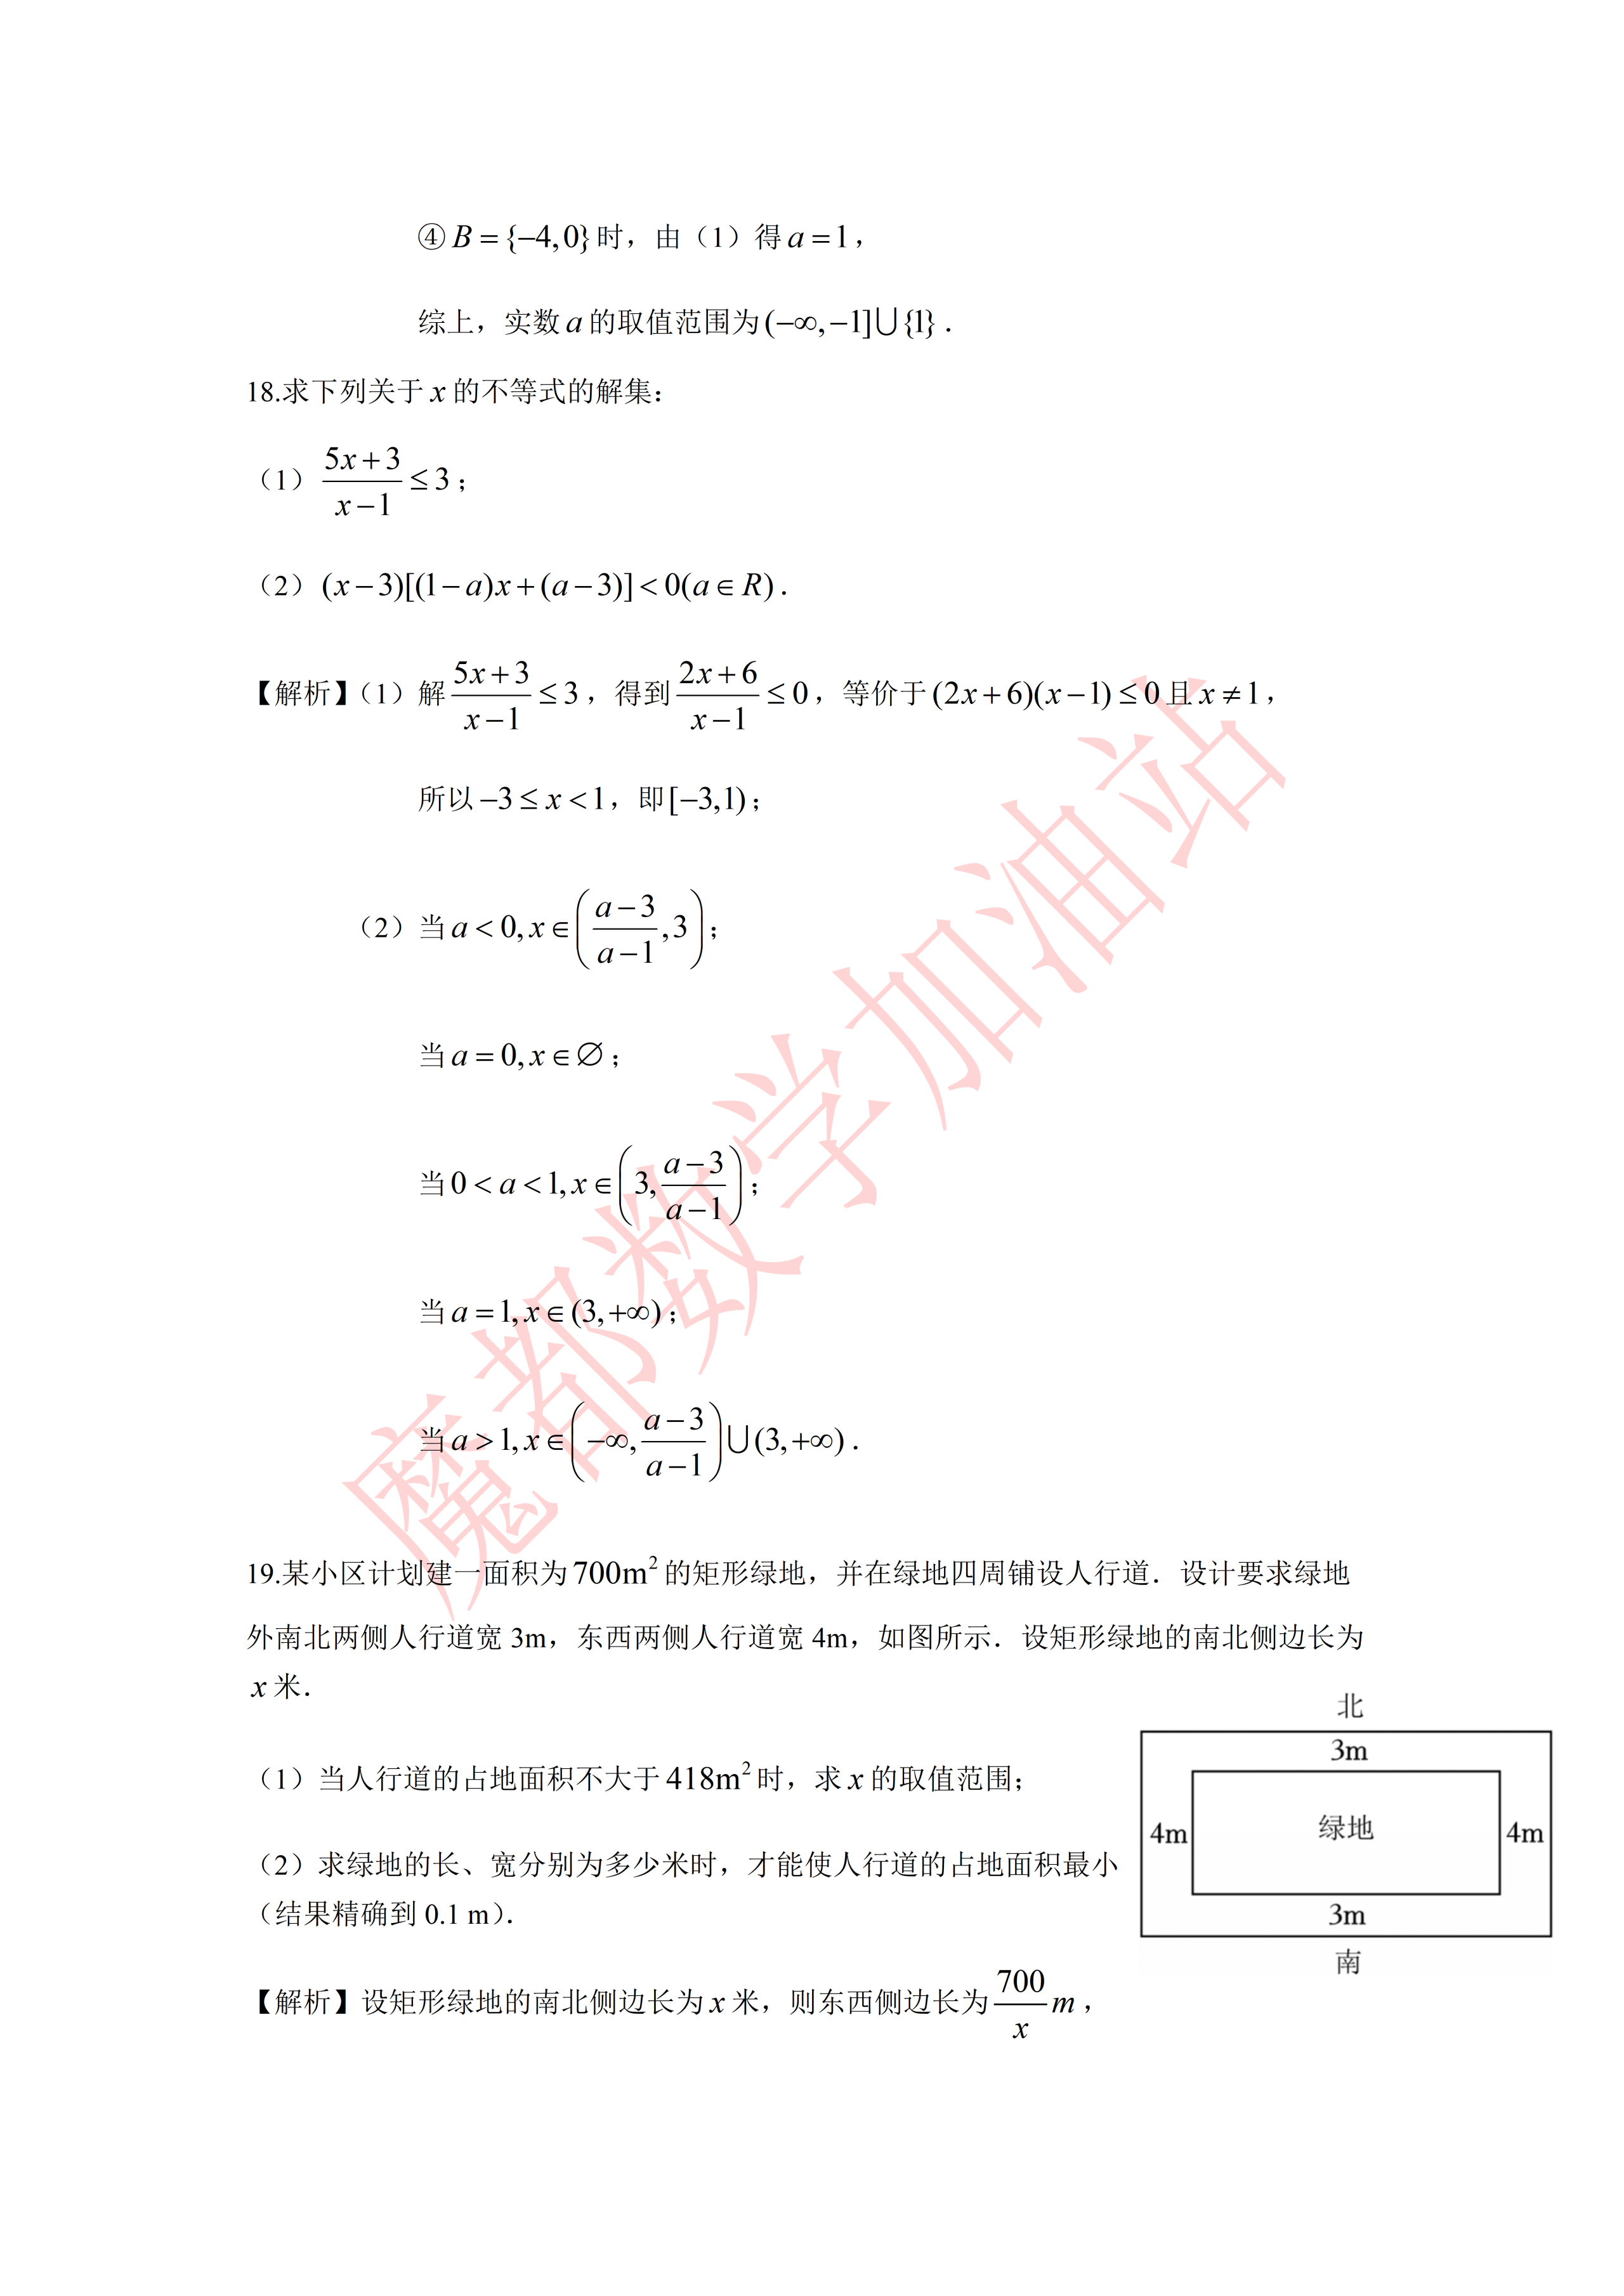
\includegraphics[width=.3\linewidth,trim=1791bp 484bp 107bp 2654bp,clip]{../原图/高一53_华师大二附中_10月月考/07.png}
\end{center}

\begin{enumerate}[label=(\arabic*)]
\item 当人行道的占地面积不大于 $418m^2$ 时，求 $x$ 的取值范围；
\item 求绿地的长、宽分别为多少米时，才能使人行道的占地面积最小（结果精确到 $0.1m$）.
\end{enumerate}

\ifanswer
\solbegin
\step{设矩形绿地的南北侧边长为 $x$ 米，则东西侧边长为 $\dfrac{700}{x}m$，}
\step{则人行道的占地面积为 $S=(x+8)\left(\dfrac{700}{x}+6\right)-700$，即 $S=6x+\dfrac{5600}{x}+48$.}
\stepm{(1)}{当人行道的占地面积不大于 $418m^2$ 时，$6x+\dfrac{5600}{x}+48\leqslant418$，}
\step{即 $6x^2-370x+5600\leqslant0$，解得 $\dfrac{80}{3}\leqslant x\leqslant35$，}
\step{故当人行道的占地面积不大于 $418m^2$ 时，$x\in\left[\dfrac{80}{3},35\right]$；}
\stepm{(2)}{$S=6x+\dfrac{5600}{x}+48\geqslant2\sqrt{6x\cdot\dfrac{5600}{x}}+48=80\sqrt{21}+48$，}
\step{当且仅当 $6x=\dfrac{5600}{x}$，即 $x=20\sqrt{\dfrac73}\approx30.6(m)$ 时，}
% 原卷如此，照录未改（80√21+48≈414.6，两处“414.4”疑笔误，见文件头“原卷笔误/存疑”第 6 条）
\step{$S$ 达到最小值 $80\sqrt{21}+48\approx414.4$，此时 $\dfrac{700}{x}\approx22.9(m)$，}
\step{所以当设计绿地的南北侧边长约为 $30.6m$，东西侧边长约为 $22.9m$ 时，}
\step{人行道的占地面积最小值为 $414.4(m^2)$.}
\solend
\fi

\ansspace[6]

\item 已知 $x\in\R$，符号 $[x]$ 表示不大于 $x$ 的最大整数，例如：$[2.3]=2$,$[2]=2$，$[-1.2]=-2$，令 $S(x)=[x]-[-x]$.

\begin{enumerate}[label=(\arabic*)]
\item 写出 $S(x)$ 为偶数（包括正、负偶数和 0）的充要条件，并证明；
\item 设方程 $|S(x)|=3$ 的解集为 $A$.

①集合 $B=\{x\mid x^2-ax-9\leqslant0,a\in\R\}$，若 $A\cap B=A$，求实数 $a$ 的取值范围；

②集合 $C=\{x\mid 2x^2-5kx+3k^2\geqslant0\}$，若 $A\cup C=\R$，求实数 $k$ 的取值范围.
\end{enumerate}

\ifanswer
\solbegin
\stepm{(1)}{$S(x)$ 为偶数的充要条件是 $x\in\Z$.}
\step{若 $x\in\Z$，则 $S(x)=[x]-[-x]=x-(-x)=2x$；}
\step{若 $x\notin\Z$，设 $[x]=n$，}
\step{则 $S(x)=[x]-[-x]=n-(-n-1)=2n+1=2[x]+1$；}
% 原卷如此，照录未改（“由①”按文意应为“由(1)”，见文件头“原卷笔误/存疑”第 3 条）
\stepm{(2)}{由①得 3 是奇数，$S(x)=\pm3$,$x\notin\Z$，}
\step{$S(x)=2[x]+1=\pm3$,$[x]=1$ 或 $-2$ 且 $x\notin\Z$，}
\step{所以 $A=(-2,-1)\cup(1,2)$；}
\stepm{①}{$A\cap B=A\Rightarrow A\subseteq B$，}
\step{设 $B=[x_1,x_2]$，其中 $x_1,x_2$ 是方程 $x^2-ax-9=0$ 的两实根，}
\step{设 $f(x)=x^2-ax-9$，}
\step{$[-2,2]\subseteq[x_1,x_2]\Leftrightarrow x_1\leqslant-2$,$x_2\geqslant2\Leftrightarrow\begin{cases}f(-2)\leqslant0\\ f(2)\leqslant0\end{cases}$}
\step{$\Leftrightarrow\begin{cases}(-2)^2-a\cdot(-2)-9\leqslant0, & a\leqslant\dfrac52\\ 2^2-2a-9\leqslant0, & a\geqslant-\dfrac52\end{cases}$，故 $a\in\left[-\dfrac52,\dfrac52\right]$；}
\step{注：若用求根公式 $\begin{cases}\dfrac{a+\sqrt{a^2+36}}{2}\geqslant2\Rightarrow a\geqslant-\dfrac52\\ \dfrac{a-\sqrt{a^2+36}}{2}\leqslant-2\Rightarrow a\leqslant\dfrac52\end{cases}$，结果正确，也得满分；}
\stepm{②}{$2x^2-5kx+3k^2=(x-k)(2x-3k)$.}
\step{$A\cup C=\R\Leftrightarrow\complement_\R A\subseteq C$.}
\step{记 $g(x)=2x^2-5kx+3k^2$，则 $\{x\mid g(x)<0\}\subseteq A$.}
\stepm{情况1：}{$k>0$ 时，$k<\dfrac32k$,$g(x)<0$ 的解集为 $\left(k,\dfrac32k\right)\subseteq(1,2)$，}
\step{故 $\begin{cases}k\geqslant1\\ \dfrac32k\leqslant2\end{cases}\Rightarrow1\leqslant k\leqslant\dfrac43$；}
\stepm{情况2：}{$k=0$ 时，$g(x)=2x^2\geqslant0$ 恒成立，$C=\R$,$A\cup C=\R$ 显然成立；}
\stepm{情况3：}{$k<0$ 时，$\dfrac32k<k$,$g(x)<0$ 的解集为 $\left(\dfrac32k,k\right)\subseteq(-2,-1)$，}
\step{故 $\begin{cases}\dfrac32k\geqslant-2\\ k\leqslant-1\end{cases}\Rightarrow-\dfrac43\leqslant k\leqslant-1$；}
\step{综上，$k\in\left[-\dfrac43,-1\right]\cup\{0\}\cup\left[1,\dfrac43\right]$.}
\solend
\fi

\ansspace[10]

\item 对于非空实数集 $M\subseteq(0,+\infty)$，若满足以下两个条件，则称 $M$ 为“极闭集”：

①$M$ 中至少含有 2 个元素，且 $1\notin M$；

②对于 $M$ 中任意两个不相等的元素 $x,y$，定义 $x*y=\dfrac{xy+1}{x+y}$，且 $x*y\in M$.

\begin{enumerate}[label=(\arabic*)]
\item 判断集合 $A=\left\{\dfrac12,2\right\}$ 与区间 $B=(1,+\infty)$ 是否为“极闭集”，并说明理由；
\item 若 $M$ 是“极闭集”，证明：集合 $M$ 中不可能所有元素都小于 1；
\item 证明：不存在任何有限的“极闭集”.
\end{enumerate}

\ifanswer
\solbegin
% 原卷如此，照录未改（首行集合按题干应为 {1/2,2}，见文件头“原卷笔误/存疑”第 7 条）
\stepm{(1)}{对于集合 $A=\left\{\dfrac12,1\right\}$，$\dfrac12*2=\dfrac45$，}
\step{因为 $\dfrac45\notin A$，不满足条件②，所以集合 $A$ 不是“极闭集”.}
\step{对于区间 $B$，满足条件①.}
\step{任取 $B$ 中两个不相等的元素 $x,y$，则 $x>1$,$y>1$.}
\step{$x*y-1=\dfrac{xy+1}{x+y}-1=\dfrac{(x-1)(y-1)}{x+y}>0$，所以 $x*y>1$，}
\step{这说明 $x*y\in B$ 恒成立，满足条件②，所以 $B$ 是“极闭集”.}
\stepm{(2)}{假设集合 $M$ 中所有元素都小于 1，}
\step{在 $M$ 中取 $0<x<y<1$,$x*y-1=\dfrac{xy+1}{x+y}-1=\dfrac{(x-1)(y-1)}{x+y}>0$，}
\step{所以 $x*y>1$，与“集合 $M$ 中所有元素都小于 1”矛盾，}
\step{假设不成立，集合 $M$ 中不可能所有元素都小于 1，得证.}
\stepm{(3)}{由②得，任何一个“极闭集”$M$ 中，必然至少存在一个大于 1 的元素，}
\stepm{情况1：}{若 $M$ 中至少存在两个大于 1 的元素，}
\step{设其中两个不相等的元素为 $x$ 和 $y_1$，且 $x>y_1>1$，}
\step{令 $y_{n+1}=x*y_n$,$n\geqslant1$,$y_{n+1}-1=x*y_n-1=\dfrac{(x-1)(y_n-1)}{xy_n+1}>0$，}
\step{如果 $y_n\geqslant1$，则显然 $y_{n+1}\geqslant1$，作差 $y_n-y_{n+1}=\dfrac{y_n^2-1}{x+y_n}>0$，}
\step{由此 $x>y_1>y_2>y_3>\cdots>1$，与有限集矛盾.}
\stepm{情况2：}{若 $M$ 中恰好只有一个元素大于 1，}
\step{设这个唯一大于 1 的元素为 $m$.}
\step{因为 $M$ 至少有两个元素，所以 $M$ 中必然至少存在一个元素 $a_1<1$，}
\step{令 $a_{n+1}=m*a_n$,$n\geqslant1$，}
\step{又 $a_{n+1}-1=m*a_n-1=\dfrac{(m-1)(a_n-1)}{m+a_n}<0$，故 $a_{n+1}<1$，}
\step{作差 $a_{n+1}-a_n=\dfrac{1-a_n^2}{m+a_n}>0$，由此 $a_1<a_2<a_3<\cdots<1$，与有限集矛盾.}
\step{因此，不存在任何有限的“极闭集”. 原命题得证.}
\solend
\fi

\ansspace*[10]

\end{enumerate}

\end{document}
"
%
% 原始材料：微信公众号“魔都数学加油站”文章，作者破晓，连载“27学年高一53”；
% 原文标题“27学年高一53——2026-2027年上海市华师大二附中高一上10月月考”；
% 原文链接：https://mp.weixin.qq.com/s/fpSnoF-gJEEWyxAoPC_bZA。
% 页面标注发布时间 2026-10-09 17:15（上海）。
% 正文为 11 张 PNG 页：第 01—06、08、10 页 4762×6735，第 07、09、11 页 2560×3620
% （**同一篇各页分辨率不同**），均按页序读取。11 页全为试卷正文页（卷首标题在第 1 页页顶，
% 卷末解答题第 21 题解析止于第 11 页），无封面页、目录页、二维码或宣传页。
% 粉色斜排“魔都数学加油站”为卷面水印，与公众号页脚一并未录入。
%
% 卷首标题：照卷面印作“2026--2027 年华师大二附中高一上 10 月月考”（公众号标题中的“上海市”
% 卷面标题行没有，本稿照卷面），年份区间按全稿惯例排 en dash。原卷只有一行标题、无副标题。
%
% 篇幅与题号：原卷自第 3 题起编号（第 1、2 题不在本卷内）。填空题 3—12（10 题）、
% 选择题 13—16（4 题）、解答题 17—21（5 题），共 19 题。本稿沿用原节与原题号，
% 只改排为全稿统一的大节样式（原卷小节标题为“一、填空题”“二、选择题”“三、解答题”）。
%
% 讲评版：原卷每题下直接印【答案】或【解析】。**第 13 题没有任何【答案】/【解析】段**，
% 答案“C”直接印在题干括号内（“一定不是(  C  )”），本稿按 高一37 第 13 题的成例把括号留空、
% 答案另提为 \ans{$C$}；其余 18 题都只印【解析】，按全稿口径这类题不另提 \ans{}——其中
% 选择题第 14、15、16 题的结论写在解析末句（“故选 B／D／C”），亦照录在解析内。
%
% 副标题：原卷未印副标题。本稿按“知识模块”口径标作“集合与常用逻辑用语、不等式”：
% 19 题中集合与常用逻辑用语 12 题（集合类 9 题——第 4、5、12、13、15、16、17、20、21 题；
% 逻辑类 3 题——第 3、9、14 题），不等式 7 题（含一元二次方程与绝对值方程：第 6、7、8、10、
% 11、18、19 题，其中第 11 题实为奇偶分析下的集合计数题，暂挂不等式），两类均超三分之一，
% 故并标。口径同 高一46、高一47、高一48、高一51、高一52。
%
% 与原卷的排版差异：
%   ① 原卷每题下直接印【解析】，本稿按全稿惯例将答案与解析置于答案版，试卷版保持干净；
%      第 13 题印在题干括号内的答案“C”同样移入 \ans{}，见上；
%   ② 原卷未印副标题，本稿按“知识模块”口径补出；
%   ③ 原卷填空横线约两个字宽，本稿按全稿惯例统一排 \blankline[4.4em]；
%      选择题的作答括号原卷排半角“(    )”，本稿按全稿惯例排 \mbox{（\quad）}；
%   ④ 原卷实数集排斜体/粗体 $R$、$\mathbf{R}$（第 4、6、7、18、20 题等处），本稿按全稿惯例
%      改用 $\R$；空集记号统一为 \varnothing；
%   ⑤ 原卷在数学式内多处用半角逗号（如 $x_1,x_2$、$|S|,|T|$、$a\neq0,c\neq0$），均照录未强改；
%      句末句点按全稿惯例排西文句点（原卷“故选 B．”一类全角句点亦从宽排作“.”）；
%   ⑥ 第 17—21 题的子问原卷各自另起一行，本稿按全稿惯例用 enumerate 的 (1)(2)(3)；
%      第 20 题 (2) 问下的①②两行是题干的一部分，照录为行首①②标号（不入 enumerate）；
%      解析中的子问标号一律用 \stepm{(1)}{…}，解析中的①②③④分情形用 \stepm{①}{…}；
%   ⑦ 第 12、20、21 题解析里的“情况1:”至“情况3:”标号原卷排**红色加粗**（全卷共 6 处），
%      全库无红色排字先例，本稿按全稿子题标号样式排 \stepm{情况1：}{…}（加粗着色、不改黑色基调），
%      冒号照原卷排全角；
%   ⑧ 第 19 题的示意图原卷排在题干右侧（与题干、(1) 问同高），本稿居中排在题干之后、
%      子问之前，并在 \item 前加 \needvspace 整块推走；图自原图第 07 页裁切（trim），不另存图片文件；
%   ⑨ 每道解答题原卷未留作答空白，本稿按全稿惯例加 \ansspace。
%
% 原卷笔误/存疑（均照录未改，正文对应处另有 % 注）：
%   1. 第 14 题解析末行“例如 $a=1$，$b=-1$，及必要性不成立”，“及”按文意应为“即”；
%   2. 第 15 题解析第 3 行 $\dfrac1{a+b\sqrt2}=\dfrac a{a^2-2b}+\left(-\dfrac b{a^2-2b}\right)\cdot\sqrt2$，
%      分母两处均作 $a^2-2b$，按通分应为 $a^2-2b^2$（结论 $C=X$ 不受影响）；
%   3. 第 20 题 (2) 问解析首行“由①得 3 是奇数”，按文意应为“由(1)得”（①是 (2) 问下自己
%      的子问标号，奇偶性结论出自 (1) 问）；
%   4. 第 11 题解析“只有奇数的有 $C_4^2+1=7$ 个”，按组合意义应为 $C_4^2+C_4^4=7$
%      （“$+1$”当指 4 个奇数全取的 1 种），数值无误；
%   5. 第 18 题 (2) 问解析“当 $a=0$,$x\in\varnothing$”，按文意应为“解集为 $\varnothing$”；
%   6. 第 19 题 (2) 问解析“$S$ 达到最小值 $80\sqrt{21}+48\approx414.4$”与末行
%      “人行道的占地面积最小值为 $414.4(m^2)$”，两处按 $80\sqrt{21}+48\approx414.6$，疑笔误；
%   7. 第 21 题 (1) 问解析首行“对于集合 $A=\left\{\frac12,1\right\}$”，按题干应为
%      $A=\left\{\frac12,2\right\}$（计算 $\frac12*2=\frac45$ 用的正是 $2$）；
%   8. 第 12 题解析“所以 $A=(-\infty,-4]\cup[2,+\infty)$”一行行末无标点，体例不一，照录。
%
% 插图：1 张，自原图裁切（无 \begin{tikzpicture} 重排）：
%   · 第 19 题绿地示意图（外矩形内套矩形“绿地”，上“北 3m”、下“南 3m”、左右各“4m”）
%     ——原图第 07 页，原卷排于题干右侧。
%     裁框：x 1797–2447、y 2660–3136（含“北”“南”标注，四周各留约 6px），
%     trim=1791bp 484bp 107bp 2654bp（左／下／右／上），页宽 2560、页高 3620。
%
\documentclass[a4paper,11pt]{article}
\usepackage{common}

\begin{document}

\examtitlest[3]{2026--2027 年华师大二附中高一上 10 月月考}{集合与常用逻辑用语、不等式}

\bigsec{一、填空题}

\begin{enumerate}
\setcounter{enumi}{2}

\item “$x=2$”是“$x^2-3x+2=0$”的\blankline[4.4em]条件.

（选择其中之一填空：充分非必要、必要非充分、充分、既非充分又非必要）

\ifanswer
\solbegin
\step{由 $x^2-3x+2=0$ 得 $x=1$ 或 $x=2$，}
\step{则“$x=2$”是“$x^2-3x+2=0$”的充分不必要条件.}
\solend
\fi

\item 已知 $R$ 是全集，集合 $A=\{y\mid y=-x^2+1,x\in\R\}$，集合 $B=\{x\mid x=3+|a|,a\in\R\}$，则 $\overline{A\cup B}=$\blankline[4.4em].

\ifanswer
\solbegin
\step{$A=\{y\mid y=-x^2+1,x\in\R\}=(-\infty,1]$，$B=\{x\mid x=3+|a|,a\in\R\}=[3,+\infty)$，}
\step{所以 $\overline{A\cup B}=(1,3)$.}
\solend
\fi

\item 已知 $a$ 为常数，集合 $A=\{x\mid x^2+x-6=0\}$，集合 $B=\{x\mid ax-2=0\}$，且 $B\subseteq A$，则 $a$ 的所有取值构成的集合为\blankline[4.4em].

\ifanswer
\solbegin
\step{集合 $A=\{-3,2\}$，因为 $B\subseteq A$，则 $B=\varnothing$，$\{-3\}$，$\{2\}$，$\{-3,2\}$，}
\step{当 $B=\varnothing$ 时，$a=0$，当 $B=\{-3\}$ 时，$a=-\dfrac23$，当 $B=\{2\}$ 时，$a=1$，}
\step{当 $B=\{-3,2\}$ 时，不成立，故 $a$ 的取值集合为 $\left\{0,-\dfrac23,1\right\}$.}
\solend
\fi

\item 设 $a\in\R$，若关于 $x$ 的不等式 $x^2-ax<0$ 的解集是区间 $(0,1)$ 的真子集，则 $a$ 的取值范围是\blankline[4.4em].

\ifanswer
\solbegin
\step{因为关于 $x$ 的不等式 $x^2-ax<0$ 的解集是区间 $(0,1)$ 的真子集，}
\step{当 $a=0$ 时，不等式的解集为 $\varnothing$，符合题意；}
\step{当 $a>0$ 时，不等式的解集为 $(0,a)$，则 $0<a<1$，}
\step{当 $a<0$ 时，不等式的解集为 $(a,0)$，不符合题意，}
\step{故 $a$ 的范围为 $[0,1)$.}
\solend
\fi

\item 设 $x\in\R$，则方程 $|2x+3|-|x-2|=|3x+1|$ 的解集为\blankline[4.4em].

\ifanswer
\solbegin
\step{当 $x\leqslant-\dfrac32$ 时，原式$\Leftrightarrow-2x-3+x-2=-3x-1\Leftrightarrow x=2$，不合题意；}
\step{当 $-\dfrac32<x\leqslant-\dfrac13$ 时，原式$\Leftrightarrow2x+3+x-2=-3x-1\Leftrightarrow x=-\dfrac13$；}
\step{当 $-\dfrac13<x\leqslant2$ 时，原式$\Leftrightarrow2x+3+x-2=3x+1\Leftrightarrow1=1$ 即恒成立；}
\step{当 $x>2$ 时，原式$\Leftrightarrow2x+3+2-x=3x+1\Leftrightarrow x=2$，不合题意；}
\step{故 $x\in\left[-\dfrac13,2\right]$.}
\solend
\fi

\item 已知关于 $x$ 的一元二次方程 $x^2+(4m+1)x+2m-1=0$．若方程的两根为 $x_1$、$x_2$，且满足 $\dfrac1{x_1}+\dfrac1{x_2}=-\dfrac12$，则实数 $m=$\blankline[4.4em].

\ifanswer
\solbegin
\step{由于判别式$\Delta=16m^2+5>0$恒成立，}
\step{不论 $m$ 为任何实数，方程总有两个不相等的实数根.}
\step{$\dfrac1{x_1}+\dfrac1{x_2}=-\dfrac12$，即 $\dfrac{x_1+x_2}{x_1x_2}=-\dfrac12$，由根与系数的关系得 $\dfrac{-4m-1}{2m-1}=-\dfrac12$，}
\step{解得 $m=-\dfrac12$.}
\solend
\fi

\item 已知 $\dfrac1{x-2}\geqslant1$ 是 $|x-a|<2$ 的充分非必要条件，则实数 $a$ 的取值范围是\blankline[4.4em].

\ifanswer
\solbegin
\step{由 $\dfrac1{x-2}\geqslant1$ 得 $\dfrac{3-x}{x-2}\geqslant0$，解得 $2<x\leqslant3$，由 $|x-a|<2$ 得 $a-2<x<a+2$，}
\step{因为 $\dfrac1{x-2}\geqslant1$ 是 $|x-a|<2$ 的充分非必要条件，}
\step{所以 $\{x\mid 2<x\leqslant3\}\subset\{x\mid a-2<x<a+2\}$，所以 $\begin{cases}a-2\leqslant2\\ a+2>3\end{cases}$，解得 $1<a\leqslant4$，}
\step{即实数 $a$ 的取值范围是 $(1,4]$.}
\solend
\fi

\item 设 $x,y\in(0,+\infty)$，且 $x+4y=1$，则 $\dfrac1x+\dfrac1y$ 的最小值为\blankline[4.4em].

\ifanswer
\solbegin
\step{因为 $\dfrac1x+\dfrac1y=(x+4y)\left(\dfrac1x+\dfrac1y\right)=5+\dfrac{4y}{x}+\dfrac{x}{y}\geqslant5+2\sqrt{\dfrac{4y}{x}\cdot\dfrac{x}{y}}=9$，}
\step{当且仅当 $\dfrac{4y}{x}=\dfrac{x}{y}$，即 $x=2y$，即 $x=\dfrac13$,$y=\dfrac16$ 时取等号，故最小值为 $9$.}
\solend
\fi

\item 设非空集合 $Q\subseteq M$，当 $Q$ 中所有元素和为偶数时（集合为单元素时和为元素本身），称 $Q$ 是 $M$ 的偶子集. 若集合 $M=\{1,2,3,4,5,6,7\}$，则其偶子集 $Q$ 的个数为\blankline[4.4em].

\ifanswer
\solbegin
\step{偶子集可以分为只有奇数、偶数及偶数个奇数和偶数的集合，}
\step{奇数有 4 个，偶数有 3 个，}
% 原卷如此，照录未改：按组合意义应为 C_4^2+C_4^4=7（“+1”当指 4 个奇数全取的 1 种），
% 见文件头“原卷笔误/存疑”第 4 条
\step{只有奇数的有 $C_4^2+1=7$ 个，只有偶数的有 $C_3^1+C_3^2+1=7$ 个，}
\step{偶数个奇数和偶数的：两奇一偶 $C_4^2\cdot C_3^1=18$ 个，两奇二偶 $C_4^2\cdot C_3^2=18$ 个，}
\step{两奇三偶 $C_4^2\cdot C_3^3=6$ 个，四奇一偶 $C_4^4\cdot C_3^1=3$ 个，四奇二偶 $C_4^4\cdot C_3^2=3$ 个，}
\step{四奇三偶 $C_4^4\cdot C_3^3=1$ 个，所以共有 $7+7+18+18+6+3+3+1=63$ 个.}
\solend
\fi

\item 已知集合 $A=\{x\mid x^2+2x-8\geqslant0\}$,$B=\{x\mid x^2-2ax+2a\leqslant0\}$，且 $A\cap B$ 中恰有 3 个整数元素，则实数 $a$ 的取值范围为\blankline[4.4em].

\ifanswer
\solbegin
% 原卷如此，照录未改：此行行末无标点，见文件头“原卷笔误/存疑”第 8 条
\step{由 $x^2+2x-8\geqslant0$，得 $x\geqslant2$ 或 $x\leqslant-4$，所以 $A=(-\infty,-4]\cup[2,+\infty)$}
\step{对集合 $B$：$x^2-2ax+2a\leqslant0$,$\Delta=4a^2-8a=4a(a-2)\geqslant0$，}
\step{得 $a\leqslant0$ 或 $a\geqslant2$.}
\step{设方程 $x^2-2ax+2a=0$ 的两根为 $r_1,r_2$，}
\step{则 $B=[r_1,r_2]$,$r_1=a-\sqrt{a^2-2a}$,$r_2=a+\sqrt{a^2-2a}$，}
\stepm{情况1：}{$a\leqslant0$，}
\step{$r_2=a+\sqrt{a^2-2a}<a+\sqrt{a^2-2a+1}=a+|a-1|=a+1-a=1<2$，}
\step{$B$ 只在 $A$ 的左侧部分有交集，要使 $A\cap B$ 恰有 3 个整数元素，}
\step{这 3 个整数为 $-6,-5,-4$，于是 $r_1\in(-7,-6]$，}
\step{令 $f(x)=x^2-2ax+2a$，则 $\begin{cases}f(-7)=49+14a+2a>0\\ f(-6)=36+12a+2a\leqslant0\end{cases}\Rightarrow a\in\left(-\dfrac{49}{16},-\dfrac{18}{7}\right]$；}
\stepm{情况2：}{$a\geqslant2$，}
\step{$r_2=a+\sqrt{a^2-2a}\geqslant2$，}
\step{$r_1=a-\sqrt{a^2-2a}>a-\sqrt{a^2-2a+1}=a-|a-1|=a-(a-1)=1>-4$，}
\step{所以 $A\cap B=[2,r_2]$.}
\step{同理 $\begin{cases}f(4)=16-8a+2a\leqslant0\\ f(5)=25-10a+2a>0\end{cases}\Rightarrow a\in\left[\dfrac{8}{3},\dfrac{25}{8}\right)$；}
\step{综上，$a\in\left(-\dfrac{49}{16},-\dfrac{18}{7}\right]\cup\left[\dfrac{8}{3},\dfrac{25}{8}\right)$.}
\solend
\fi

\end{enumerate}

\bigsec{二、选择题}

\begin{enumerate}
\setcounter{enumi}{12}

% 第 13 题原卷无【答案】/【解析】段，答案“C”直接印在题干括号内，
% 按高一37 第 13 题的成例括号留空、答案另提为 \ans{}（见文件头）
\item 集合 $A=\{a,b,c\}$ 中的三个元素分别表示某一个三角形的三边长度，那么这个三角形一定不是\mbox{（\quad）}

\keepwithprev
A. 锐角三角形\qquad B. 钝角三角形

C. 等腰三角形\qquad D. 直角三角形

\ifanswer
\ans{$C$}
\fi

\item 设 $a$、$b$ 为实数，则“$a<b<0$”是“$\dfrac1a>\dfrac1b$”的\mbox{（\quad）}条件.

\keepwithprev
A. 充要\qquad B. 充分不必要

C. 必要不充分\qquad D. 既不充分也不必要

\ifanswer
\solbegin
\step{若 $a<b<0$，则 $\dfrac1a>\dfrac1b$ 一定成立，即充分性成立；}
% 原卷如此，照录未改（“及”按文意应为“即”，见文件头“原卷笔误/存疑”第 1 条）
\step{若 $\dfrac1a>\dfrac1b$ 成立，$a<b<0$ 不一定成立，例如 $a=1$，$b=-1$，及必要性不成立.}
\step{故选 $B$.}
\solend
\fi

\item 设 $Q$ 表示有理数集，集合 $X=\{x\mid x=a+b\sqrt2,a,b\in Q,x\neq0\}$，在下列集合中：①$\{2x\mid x\in X\}$②$\left\{\dfrac{x}{\sqrt2}\mid x\in X\right\}$③$\left\{\dfrac1x\mid x\in X\right\}$④$\{x^2\mid x\in X\}$，与 $X$ 相同的集合有\mbox{（\quad）}

\keepwithprev
A. ①②③④\qquad B. ②③④\qquad C. ①②④\qquad D. ①②③

\ifanswer
\solbegin
\step{$A=\{2x\mid x\in X\}$，$2(a+b\sqrt2)=p+q\sqrt2$ 得 $p=2a$，$q=2b$，$a=\dfrac p2$，$b=\dfrac q2$，}
\step{也是一一对应，$A=X$}
% 原卷如此，照录未改：分母两处均作 a^2-2b，按通分应为 a^2-2b^2，
% 见文件头“原卷笔误/存疑”第 2 条
\step{集合 $B=\left\{\dfrac{x}{\sqrt2}\mid x\in X\right\}$，$\dfrac{a+b\sqrt2}{\sqrt2}=b+\dfrac a2\cdot\sqrt2$，也是一一对应，$B=X$}
\step{集合 $C=\left\{\dfrac1x\mid x\in X\right\}$，$\dfrac{1}{a+b\sqrt2}=\dfrac{a}{a^2-2b}+\left(-\dfrac{b}{a^2-2b}\right)\cdot\sqrt2$，一一对应，$C=X$}
\step{集合 $D=\{x^2\mid x\in X\}$，$(a+b\sqrt2)^2=a^2+2b^2+2ab\sqrt2$，这个不能一一对应了，}
\step{集合 $D$ 包含于 $X$ 中.}
\step{故 $X$ 相同的集合有①②③，故选 $D$.}
\solend
\fi

\item 集合 $S=\{x\mid(x+a)(x^2+bx+c)=0\}$,$T=\{x\mid(ax+1)(cx^2+bx+1)=0\}$，其中 $a,b,c$ 为实数，若 $|S|,|T|$ 分别表示集合 $S,T$ 的元素个数，则 $|S|-|T|$ 的所有可能取值集合为\mbox{（\quad）}

\keepwithprev
A. $\{0\}$\qquad B. $\{1\}$\qquad C. $\{0,1\}$\qquad D. $\{-1,0,1\}$

\ifanswer
\solbegin
\stepm{①}{$a\neq0,c\neq0$ 时.}
\step{$S$ 中 $x+a=0$ 的根 $x=-a$;$T$ 中 $ax+1=0$ 的根 $x=-\dfrac1a$.}
\step{$S$ 中的 $x^2+bx+c=0$ 若无实根，则 $T$ 中的 $cx^2+bx+1=0$ 也无实根；}
\step{又设 $S$ 的 $x^2+bx+c=0$ 的根为 $r(r\neq0)$，则 $T$ 的 $cx^2+bx+1=0$ 的根为 $\dfrac1r$.}
\step{（因为 $r^2+br+c=0\Rightarrow c\cdot\left(\dfrac1r\right)^2+b\cdot\dfrac1r+1=0$）}
\step{即 $a\neq0,c\neq0$ 时，}
\step{$S$ 与 $T$ 的实根存在一一对应关系 $x\leftrightarrow\dfrac1x$,$|S|=|T|,$$|S|-|T|=0$；}
\stepm{②}{$a=0,c\neq0$ 时.}
\step{$S$ 中多出一个根 $x=0$，而 $T$ 中无此根，$|S|=|T|+1$，即 $|S|-|T|=1$；}
\stepm{③}{$a\neq0,c=0$ 时.}
\step{则 $S$ 中仍有根 $x=0$，而 $T$ 中无 0 根，同样 $|S|-|T|=1$.}
\stepm{④}{$a=0,c=0$ 时.}
\step{同样 $S$ 含有根 0，而 $T$ 中不含 0，仍有 $|S|-|T|=1$.}
\step{综上，$|S|-|T|$ 所有可能取值为 0 和 1，故选 $C$.}
\solend
\fi

\end{enumerate}

\bigsec{三、解答题}

\begin{enumerate}
\setcounter{enumi}{16}

\item 已知集合 $A=\{x\mid x^2+4x=0\}$，$B=\{x\mid x^2+2(a+1)x+a^2-1=0\}$.

\begin{enumerate}[label=(\arabic*)]
\item 若 $A$ 是 $B$ 的子集，求实数 $a$ 的值；
\item 若 $B$ 是 $A$ 的子集，求实数 $a$ 的取值范围.
\end{enumerate}

\ifanswer
\solbegin
\stepm{(1)}{因为 $A=\{-4,0\}$，$B=\{x\mid x^2+2(a+1)x+a^2-1=0\}$，又 $A\subseteq B$，}
\step{所以 $A=B$，所以 $\begin{cases}-4+0=-2(a+1)\\ -4\times0=a^2-1\end{cases}$，所以 $a=1$；}
\stepm{(2)}{因为 $B$ 是 $A$ 的子集，所以 $B=\varnothing$ 或 $B=\{-4\}$ 或 $B=\{0\}$ 或 $B=\{-4,0\}$，}
\stepm{①}{$B=\varnothing$ 时，$\Delta=4(a+1)^2-4(a^2-1)<0$，所以 $a<-1$；}
\stepm{②}{$B=\{-4\}$ 时，$\begin{cases}-4+(-4)=-2(a+1)\\ -4\times(-4)=a^2-1\end{cases}$，无解；}
\stepm{③}{$B=\{0\}$ 时，$\begin{cases}0+0=-2(a+1)\\ 0\times0=a^2-1\end{cases}$，所以 $a=-1$；}
\stepm{④}{$B=\{-4,0\}$ 时，由（1）得 $a=1$，}
\step{综上，实数 $a$ 的取值范围为 $(-\infty,-1]\cup\{1\}$.}
\solend
\fi

\ansspace[6]

\item 求下列关于 $x$ 的不等式的解集：

\begin{enumerate}[label=(\arabic*)]
\item $\dfrac{5x+3}{x-1}\leqslant3$；
\item $(x-3)[(1-a)x+(a-3)]<0$ ($a\in\R$).
\end{enumerate}

\ifanswer
\solbegin
\stepm{(1)}{解 $\dfrac{5x+3}{x-1}\leqslant3$，得到 $\dfrac{2x+6}{x-1}\leqslant0$，等价于 $(2x+6)(x-1)\leqslant0$ 且 $x\neq1$，}
\step{所以 $-3\leqslant x<1$，即 $[-3,1)$；}
\stepm{(2)}{当 $a<0$,$x\in\left(\dfrac{a-3}{a-1},3\right)$；}
% 原卷如此，照录未改（“x∈∅”按文意应为“解集为 ∅”，见文件头“原卷笔误/存疑”第 5 条）
\step{当 $a=0$,$x\in\varnothing$；}
\step{当 $0<a<1$,$x\in\left(3,\dfrac{a-3}{a-1}\right)$；}
\step{当 $a=1$,$x\in(3,+\infty)$；}
\step{当 $a>1$,$x\in\left(-\infty,\dfrac{a-3}{a-1}\right)\cup(3,+\infty)$.}
\solend
\fi

\ansspace[6]

\needvspace{13\baselineskip}

\item 某小区计划建一面积为 $700m^2$ 的矩形绿地，并在绿地四周铺设人行道. 设计要求绿地外南北两侧人行道宽 $3m$，东西两侧人行道宽 $4m$，如图所示. 设矩形绿地的南北侧边长为 $x$ 米.

\begin{center}
% 原图第 7 页题干绿地示意图直接裁取（原卷排于题干右侧）。
% 裁框取图形外框 x 1797–2447、y 2660–3136（含“北”“南”标注，四周各留约 6px），
% trim=左 1791bp／下 484bp／右 107bp／上 2654bp（页宽 2560、页高 3620）。
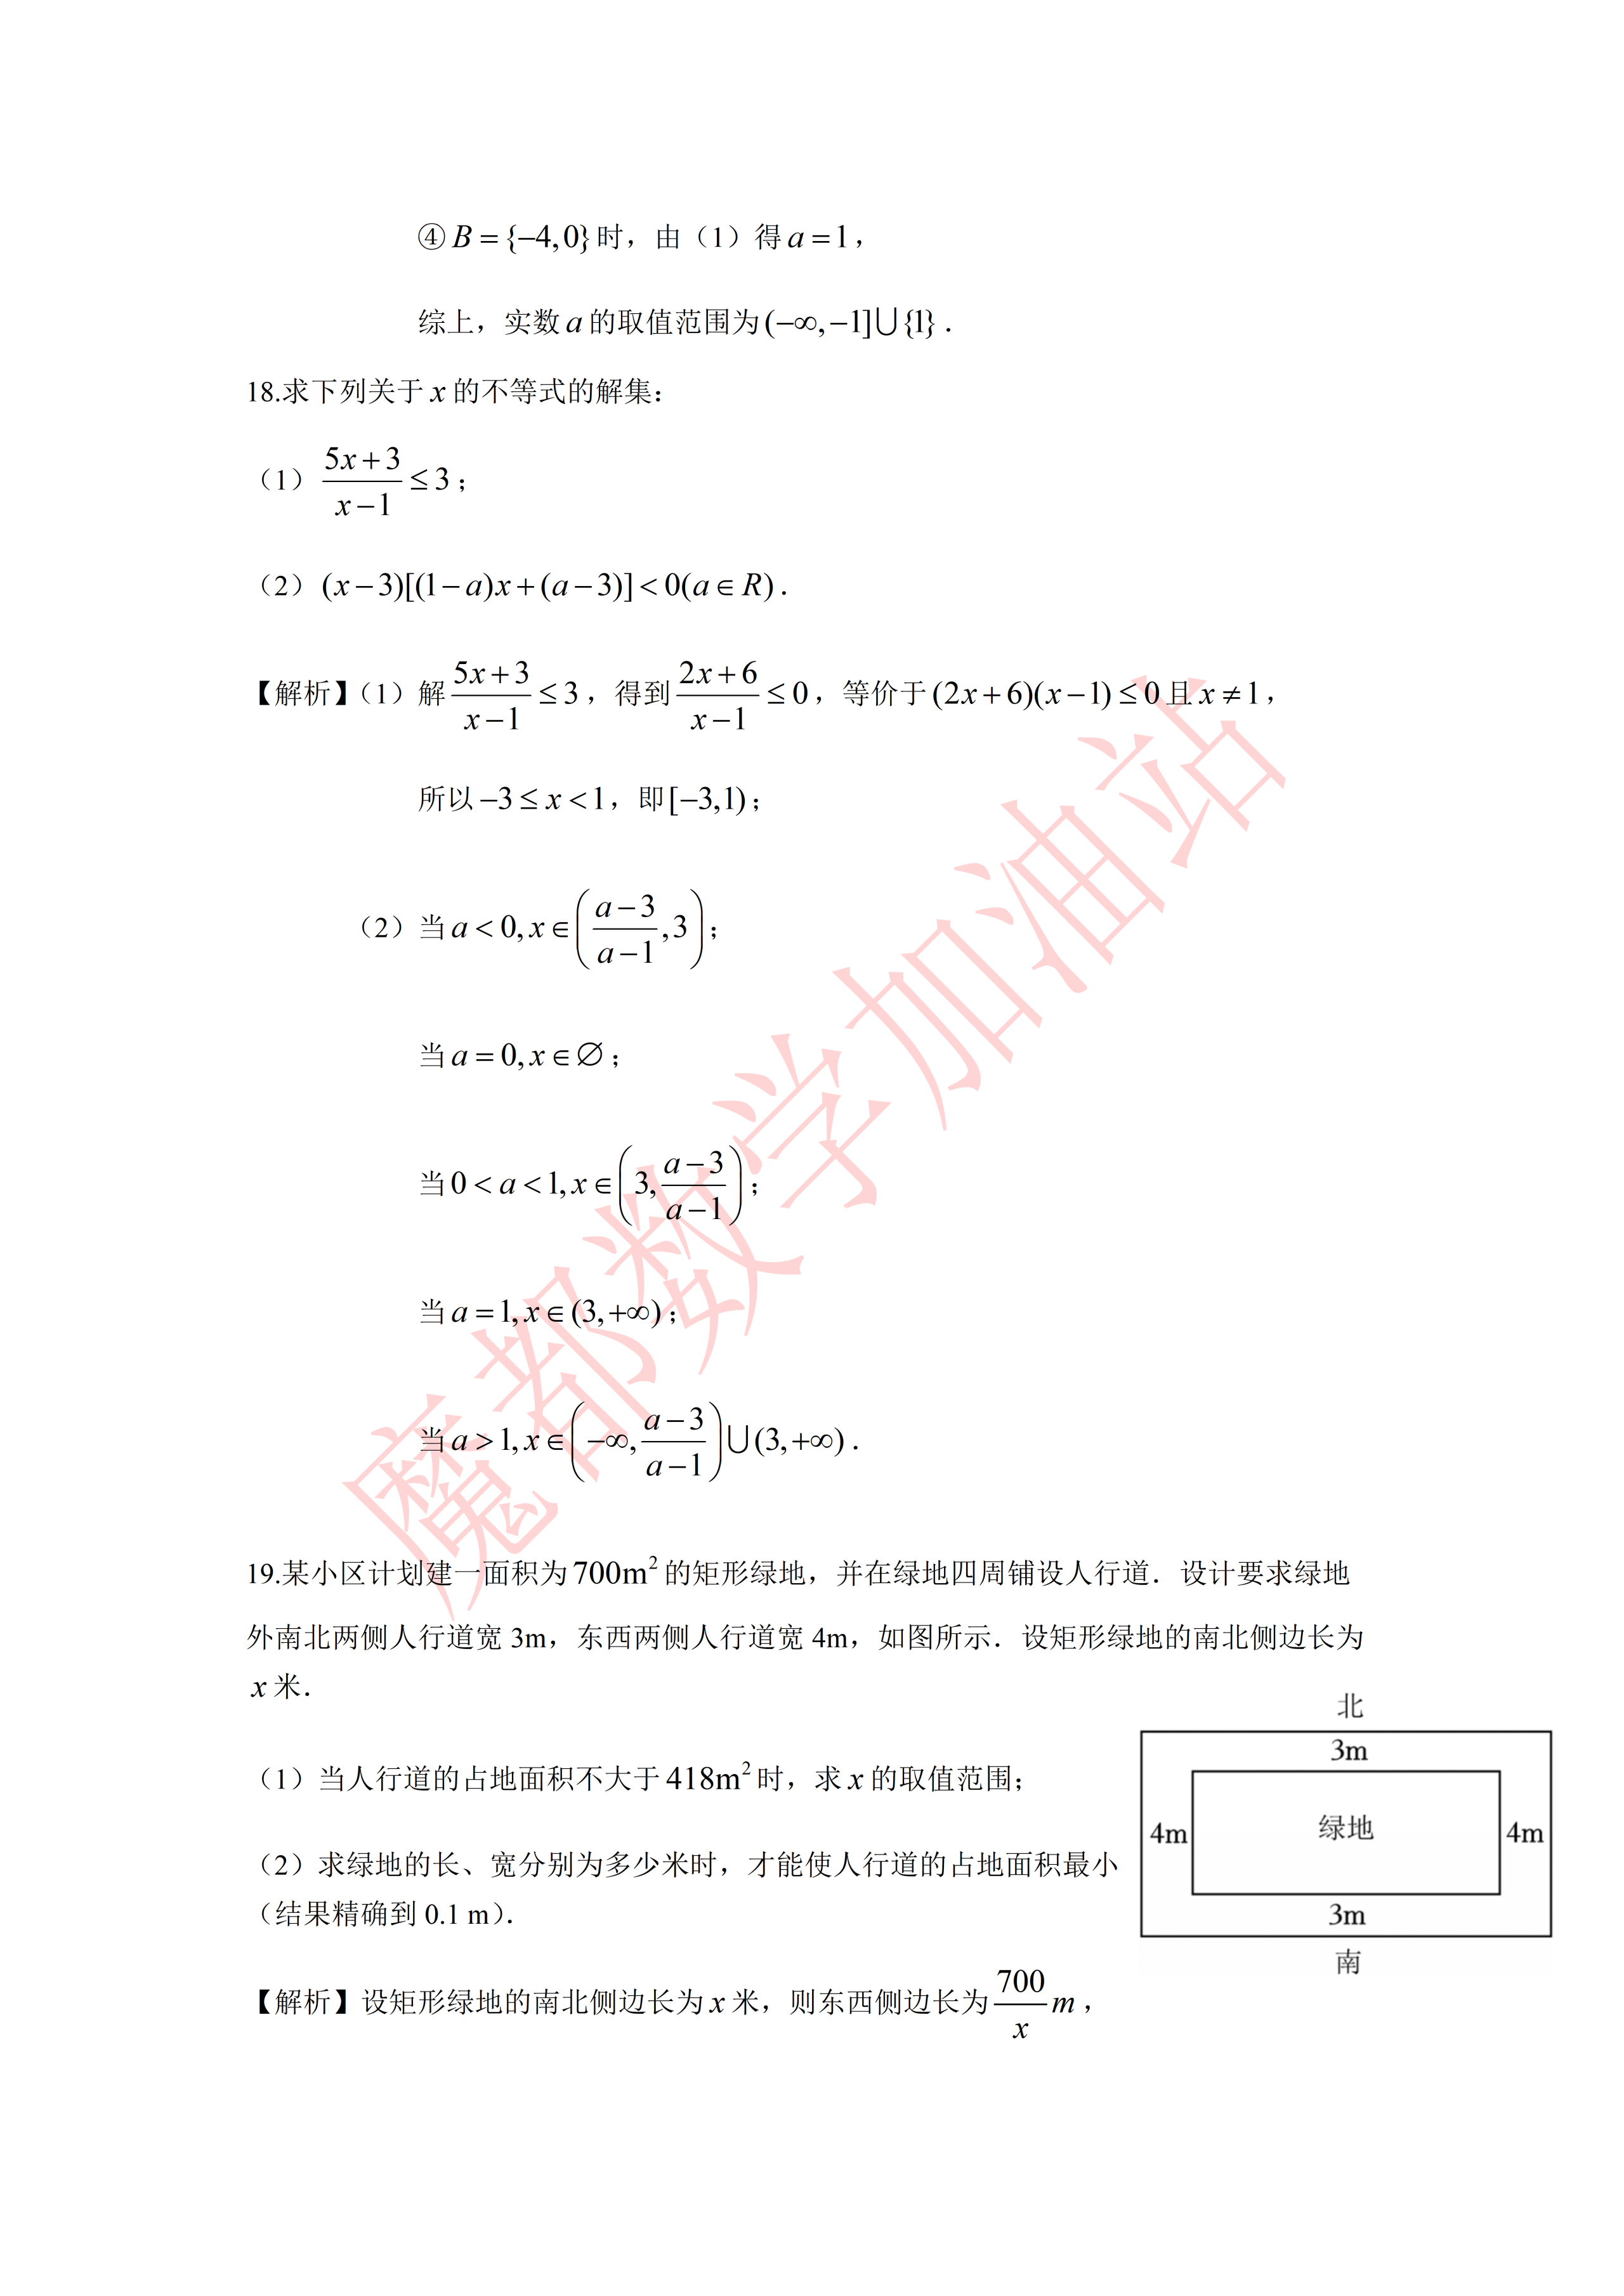
\includegraphics[width=.3\linewidth,trim=1791bp 484bp 107bp 2654bp,clip]{../原图/高一53_华师大二附中_10月月考/07.png}
\end{center}

\begin{enumerate}[label=(\arabic*)]
\item 当人行道的占地面积不大于 $418m^2$ 时，求 $x$ 的取值范围；
\item 求绿地的长、宽分别为多少米时，才能使人行道的占地面积最小（结果精确到 $0.1m$）.
\end{enumerate}

\ifanswer
\solbegin
\step{设矩形绿地的南北侧边长为 $x$ 米，则东西侧边长为 $\dfrac{700}{x}m$，}
\step{则人行道的占地面积为 $S=(x+8)\left(\dfrac{700}{x}+6\right)-700$，即 $S=6x+\dfrac{5600}{x}+48$.}
\stepm{(1)}{当人行道的占地面积不大于 $418m^2$ 时，$6x+\dfrac{5600}{x}+48\leqslant418$，}
\step{即 $6x^2-370x+5600\leqslant0$，解得 $\dfrac{80}{3}\leqslant x\leqslant35$，}
\step{故当人行道的占地面积不大于 $418m^2$ 时，$x\in\left[\dfrac{80}{3},35\right]$；}
\stepm{(2)}{$S=6x+\dfrac{5600}{x}+48\geqslant2\sqrt{6x\cdot\dfrac{5600}{x}}+48=80\sqrt{21}+48$，}
\step{当且仅当 $6x=\dfrac{5600}{x}$，即 $x=20\sqrt{\dfrac73}\approx30.6(m)$ 时，}
% 原卷如此，照录未改（80√21+48≈414.6，两处“414.4”疑笔误，见文件头“原卷笔误/存疑”第 6 条）
\step{$S$ 达到最小值 $80\sqrt{21}+48\approx414.4$，此时 $\dfrac{700}{x}\approx22.9(m)$，}
\step{所以当设计绿地的南北侧边长约为 $30.6m$，东西侧边长约为 $22.9m$ 时，}
\step{人行道的占地面积最小值为 $414.4(m^2)$.}
\solend
\fi

\ansspace[6]

\item 已知 $x\in\R$，符号 $[x]$ 表示不大于 $x$ 的最大整数，例如：$[2.3]=2$,$[2]=2$，$[-1.2]=-2$，令 $S(x)=[x]-[-x]$.

\begin{enumerate}[label=(\arabic*)]
\item 写出 $S(x)$ 为偶数（包括正、负偶数和 0）的充要条件，并证明；
\item 设方程 $|S(x)|=3$ 的解集为 $A$.

①集合 $B=\{x\mid x^2-ax-9\leqslant0,a\in\R\}$，若 $A\cap B=A$，求实数 $a$ 的取值范围；

②集合 $C=\{x\mid 2x^2-5kx+3k^2\geqslant0\}$，若 $A\cup C=\R$，求实数 $k$ 的取值范围.
\end{enumerate}

\ifanswer
\solbegin
\stepm{(1)}{$S(x)$ 为偶数的充要条件是 $x\in\Z$.}
\step{若 $x\in\Z$，则 $S(x)=[x]-[-x]=x-(-x)=2x$；}
\step{若 $x\notin\Z$，设 $[x]=n$，}
\step{则 $S(x)=[x]-[-x]=n-(-n-1)=2n+1=2[x]+1$；}
% 原卷如此，照录未改（“由①”按文意应为“由(1)”，见文件头“原卷笔误/存疑”第 3 条）
\stepm{(2)}{由①得 3 是奇数，$S(x)=\pm3$,$x\notin\Z$，}
\step{$S(x)=2[x]+1=\pm3$,$[x]=1$ 或 $-2$ 且 $x\notin\Z$，}
\step{所以 $A=(-2,-1)\cup(1,2)$；}
\stepm{①}{$A\cap B=A\Rightarrow A\subseteq B$，}
\step{设 $B=[x_1,x_2]$，其中 $x_1,x_2$ 是方程 $x^2-ax-9=0$ 的两实根，}
\step{设 $f(x)=x^2-ax-9$，}
\step{$[-2,2]\subseteq[x_1,x_2]\Leftrightarrow x_1\leqslant-2$,$x_2\geqslant2\Leftrightarrow\begin{cases}f(-2)\leqslant0\\ f(2)\leqslant0\end{cases}$}
\step{$\Leftrightarrow\begin{cases}(-2)^2-a\cdot(-2)-9\leqslant0, & a\leqslant\dfrac52\\ 2^2-2a-9\leqslant0, & a\geqslant-\dfrac52\end{cases}$，故 $a\in\left[-\dfrac52,\dfrac52\right]$；}
\step{注：若用求根公式 $\begin{cases}\dfrac{a+\sqrt{a^2+36}}{2}\geqslant2\Rightarrow a\geqslant-\dfrac52\\ \dfrac{a-\sqrt{a^2+36}}{2}\leqslant-2\Rightarrow a\leqslant\dfrac52\end{cases}$，结果正确，也得满分；}
\stepm{②}{$2x^2-5kx+3k^2=(x-k)(2x-3k)$.}
\step{$A\cup C=\R\Leftrightarrow\complement_\R A\subseteq C$.}
\step{记 $g(x)=2x^2-5kx+3k^2$，则 $\{x\mid g(x)<0\}\subseteq A$.}
\stepm{情况1：}{$k>0$ 时，$k<\dfrac32k$,$g(x)<0$ 的解集为 $\left(k,\dfrac32k\right)\subseteq(1,2)$，}
\step{故 $\begin{cases}k\geqslant1\\ \dfrac32k\leqslant2\end{cases}\Rightarrow1\leqslant k\leqslant\dfrac43$；}
\stepm{情况2：}{$k=0$ 时，$g(x)=2x^2\geqslant0$ 恒成立，$C=\R$,$A\cup C=\R$ 显然成立；}
\stepm{情况3：}{$k<0$ 时，$\dfrac32k<k$,$g(x)<0$ 的解集为 $\left(\dfrac32k,k\right)\subseteq(-2,-1)$，}
\step{故 $\begin{cases}\dfrac32k\geqslant-2\\ k\leqslant-1\end{cases}\Rightarrow-\dfrac43\leqslant k\leqslant-1$；}
\step{综上，$k\in\left[-\dfrac43,-1\right]\cup\{0\}\cup\left[1,\dfrac43\right]$.}
\solend
\fi

\ansspace[10]

\item 对于非空实数集 $M\subseteq(0,+\infty)$，若满足以下两个条件，则称 $M$ 为“极闭集”：

①$M$ 中至少含有 2 个元素，且 $1\notin M$；

②对于 $M$ 中任意两个不相等的元素 $x,y$，定义 $x*y=\dfrac{xy+1}{x+y}$，且 $x*y\in M$.

\begin{enumerate}[label=(\arabic*)]
\item 判断集合 $A=\left\{\dfrac12,2\right\}$ 与区间 $B=(1,+\infty)$ 是否为“极闭集”，并说明理由；
\item 若 $M$ 是“极闭集”，证明：集合 $M$ 中不可能所有元素都小于 1；
\item 证明：不存在任何有限的“极闭集”.
\end{enumerate}

\ifanswer
\solbegin
% 原卷如此，照录未改（首行集合按题干应为 {1/2,2}，见文件头“原卷笔误/存疑”第 7 条）
\stepm{(1)}{对于集合 $A=\left\{\dfrac12,1\right\}$，$\dfrac12*2=\dfrac45$，}
\step{因为 $\dfrac45\notin A$，不满足条件②，所以集合 $A$ 不是“极闭集”.}
\step{对于区间 $B$，满足条件①.}
\step{任取 $B$ 中两个不相等的元素 $x,y$，则 $x>1$,$y>1$.}
\step{$x*y-1=\dfrac{xy+1}{x+y}-1=\dfrac{(x-1)(y-1)}{x+y}>0$，所以 $x*y>1$，}
\step{这说明 $x*y\in B$ 恒成立，满足条件②，所以 $B$ 是“极闭集”.}
\stepm{(2)}{假设集合 $M$ 中所有元素都小于 1，}
\step{在 $M$ 中取 $0<x<y<1$,$x*y-1=\dfrac{xy+1}{x+y}-1=\dfrac{(x-1)(y-1)}{x+y}>0$，}
\step{所以 $x*y>1$，与“集合 $M$ 中所有元素都小于 1”矛盾，}
\step{假设不成立，集合 $M$ 中不可能所有元素都小于 1，得证.}
\stepm{(3)}{由②得，任何一个“极闭集”$M$ 中，必然至少存在一个大于 1 的元素，}
\stepm{情况1：}{若 $M$ 中至少存在两个大于 1 的元素，}
\step{设其中两个不相等的元素为 $x$ 和 $y_1$，且 $x>y_1>1$，}
\step{令 $y_{n+1}=x*y_n$,$n\geqslant1$,$y_{n+1}-1=x*y_n-1=\dfrac{(x-1)(y_n-1)}{xy_n+1}>0$，}
\step{如果 $y_n\geqslant1$，则显然 $y_{n+1}\geqslant1$，作差 $y_n-y_{n+1}=\dfrac{y_n^2-1}{x+y_n}>0$，}
\step{由此 $x>y_1>y_2>y_3>\cdots>1$，与有限集矛盾.}
\stepm{情况2：}{若 $M$ 中恰好只有一个元素大于 1，}
\step{设这个唯一大于 1 的元素为 $m$.}
\step{因为 $M$ 至少有两个元素，所以 $M$ 中必然至少存在一个元素 $a_1<1$，}
\step{令 $a_{n+1}=m*a_n$,$n\geqslant1$，}
\step{又 $a_{n+1}-1=m*a_n-1=\dfrac{(m-1)(a_n-1)}{m+a_n}<0$，故 $a_{n+1}<1$，}
\step{作差 $a_{n+1}-a_n=\dfrac{1-a_n^2}{m+a_n}>0$，由此 $a_1<a_2<a_3<\cdots<1$，与有限集矛盾.}
\step{因此，不存在任何有限的“极闭集”. 原命题得证.}
\solend
\fi

\ansspace*[10]

\end{enumerate}

\end{document}
